% ============================================================
%  BioPhasor: Phasor Based Cellular Dynamics and Multi-Omics Integration
%  Research-paper format (REVTeX 4-2).
% ============================================================
\documentclass[preprint,12pt,amsmath,amssymb,superscriptaddress,floatfix]{revtex4-2}

% --- Packages ---
\usepackage[T1]{fontenc}
\usepackage{amsmath, amssymb, amsfonts, amsthm}
\usepackage{graphicx}
\usepackage{subcaption}
\graphicspath{{./}}
\usepackage{float}
\usepackage{hyperref}
\usepackage{cleveref}
\usepackage{booktabs}
\usepackage{multirow}
\usepackage{listings}
\usepackage{xcolor}
\usepackage{bm}
\usepackage{braket}
\usepackage{tikz}

% --- Code Listing Style ---
\definecolor{codegreen}{rgb}{0,0.6,0}
\definecolor{codegray}{rgb}{0.5,0.5,0.5}
\definecolor{codepurple}{rgb}{0.58,0,0.82}
\definecolor{backcolour}{rgb}{0.97,0.97,0.97}

\lstdefinestyle{pythonstyle}{
    backgroundcolor=\color{backcolour},
    commentstyle=\color{codegreen},
    keywordstyle=\color{blue},
    numberstyle=\tiny\color{codegray},
    stringstyle=\color{codepurple},
    basicstyle=\ttfamily\small,
    breakatwhitespace=false,
    breaklines=true,
    captionpos=b,
    keepspaces=true,
    numbers=left,
    numbersep=5pt,
    showspaces=false,
    showstringspaces=false,
    showtabs=false,
    tabsize=2,
    language=Python
}
\lstset{style=pythonstyle}

% --- Hyperref Setup ---
\definecolor{pfblue}{RGB}{0,82,155}
\definecolor{pforange}{RGB}{200,80,0}
\hypersetup{
    colorlinks=true,
    linkcolor=pfblue,
    citecolor=pforange,
    urlcolor=pfblue
}

% --- Custom Commands ---
\newcommand{\phasorstate}[1]{\boldsymbol{z}_{#1}}
\newcommand{\reals}{\mathbb{R}}
\newcommand{\complex}{\mathbb{C}}
\newcommand{\unitary}{\mathrm{U}}

% --- Theorem Environments ---
\newtheorem{definition}{Definition}[section]
\newtheorem{theorem}{Theorem}[section]
\newtheorem{proposition}{Proposition}[section]
\newtheorem{corollary}[theorem]{Corollary}
\newtheorem{remark}{Remark}[section]

% ====================================================================

% --- Manuscript-specific: TikZ libraries & pgfplots ---
\usetikzlibrary{
  calc, shapes.geometric, shapes.misc,
  backgrounds, arrows.meta, positioning,
  decorations.pathreplacing, decorations.markings,
  fit, matrix, patterns
}
\usepackage{pgfplots}
\pgfplotsset{compat=1.18}
\usepackage{rotating}

% --- Manuscript-specific: shared omics color palette ---
\definecolor{colRNA}{HTML}{E53935}      % mRNA / Transcriptomics  — red
\definecolor{colEpi}{HTML}{8E24AA}      % Epigenomics / Methylation — purple
\definecolor{colChrom}{HTML}{43A047}    % Chromatin / ATAC-seq — green
\definecolor{colTF}{HTML}{1E88E5}       % TF Binding / Proteomics — blue
\definecolor{colNeutral}{HTML}{757575}  % Neutral annotations — gray
\definecolor{colCoher}{HTML}{FB8C00}    % Coherence highlight — orange

% --- Manuscript-specific: additional custom commands ---
\newcommand{\torus}{\mathbb{T}}
\newcommand{\coherence}{\mathcal{C}}


\begin{document}

% --- BEGIN sections/abstract.tex ---
% sections/abstract.tex

\title{BioPhasor: A Phase-Geometric Platform for Decoding Cellular State Tensors from Multi-Omics, toward Quantum-Ready Systems Biology}

\author{Dibakar Sigdel}
\email{devdeep137@gmail.com}
\affiliation{Mindverse Computing LLC, Lynnwood, WA 98087}
\author{Namuna Panday}
\affiliation{Mindverse Computing LLC, Lynnwood, WA 98087}

\date{\today}

\begin{abstract}
Linear embeddings routinely used to summarise multi-omics data (PCA, NMF)
discard the phase structure of intrinsically oscillatory molecular programs. We
present \textbf{BioPhasor}, a phase-geometric platform that encodes each
measurement as a complex phasor $\psi = r\,e^{i\theta}$ on the $N$-torus
$\mathbb{T}^N$ and decodes the Cell State Tensor (CST)---an order-3 latent field
over regulatory, temporal, and homeostatic axes---from multi-omics phasor
dynamics. The CST's regulatory structure is a \emph{phase-coherence density
matrix} $\rho=\frac1M\sum_m\boldsymbol z_m\boldsymbol z_m^{\dagger}$, whose
off-diagonals are phase-locking values. Because $\rho$ is a bona-fide density
operator, the CST is natively \emph{quantum-ready}: its descriptors and its
Variational Phasor Circuit map exactly onto density-operator and
variational-quantum-circuit constructs---an exact
classical$\leftrightarrow$quantum correspondence, no quantum advantage claimed. BioPhasor is released as a phase-native API spanning encoding, circular and
Riemannian statistics, Kuramoto dynamics, the CST, and a variational phasor
circuit, and demonstrated across nine illustrative applications on real public
data, each with an honest reproduces/partial/does-not-reproduce verdict that
scopes where a phase view helps and where it does not. One vignette illustrates
end-to-end phase--amplitude coupling on a matched CPTAC endometrial-carcinoma
cohort ($z=180$; tumour-specific, $r=0.29$ vs $0.03$), developed fully in a
companion study. A single loader regenerates every reported number.
\end{abstract}

\keywords{cell state tensor, multi-omics integration, phasor encoding, phase coherence, phase-coherence density matrix, quantum-ready systems biology, variational quantum circuit, classical--quantum correspondence, phase--amplitude coupling, central dogma, circular statistics, Kuramoto dynamics, circadian rhythms, systems biology, BioPhasor}

\maketitle

% --- END sections/abstract.tex ---

% --- BEGIN sections/introduction.tex ---
% introduction.tex
\section{Introduction}

\begin{figure*}[t]
\centering
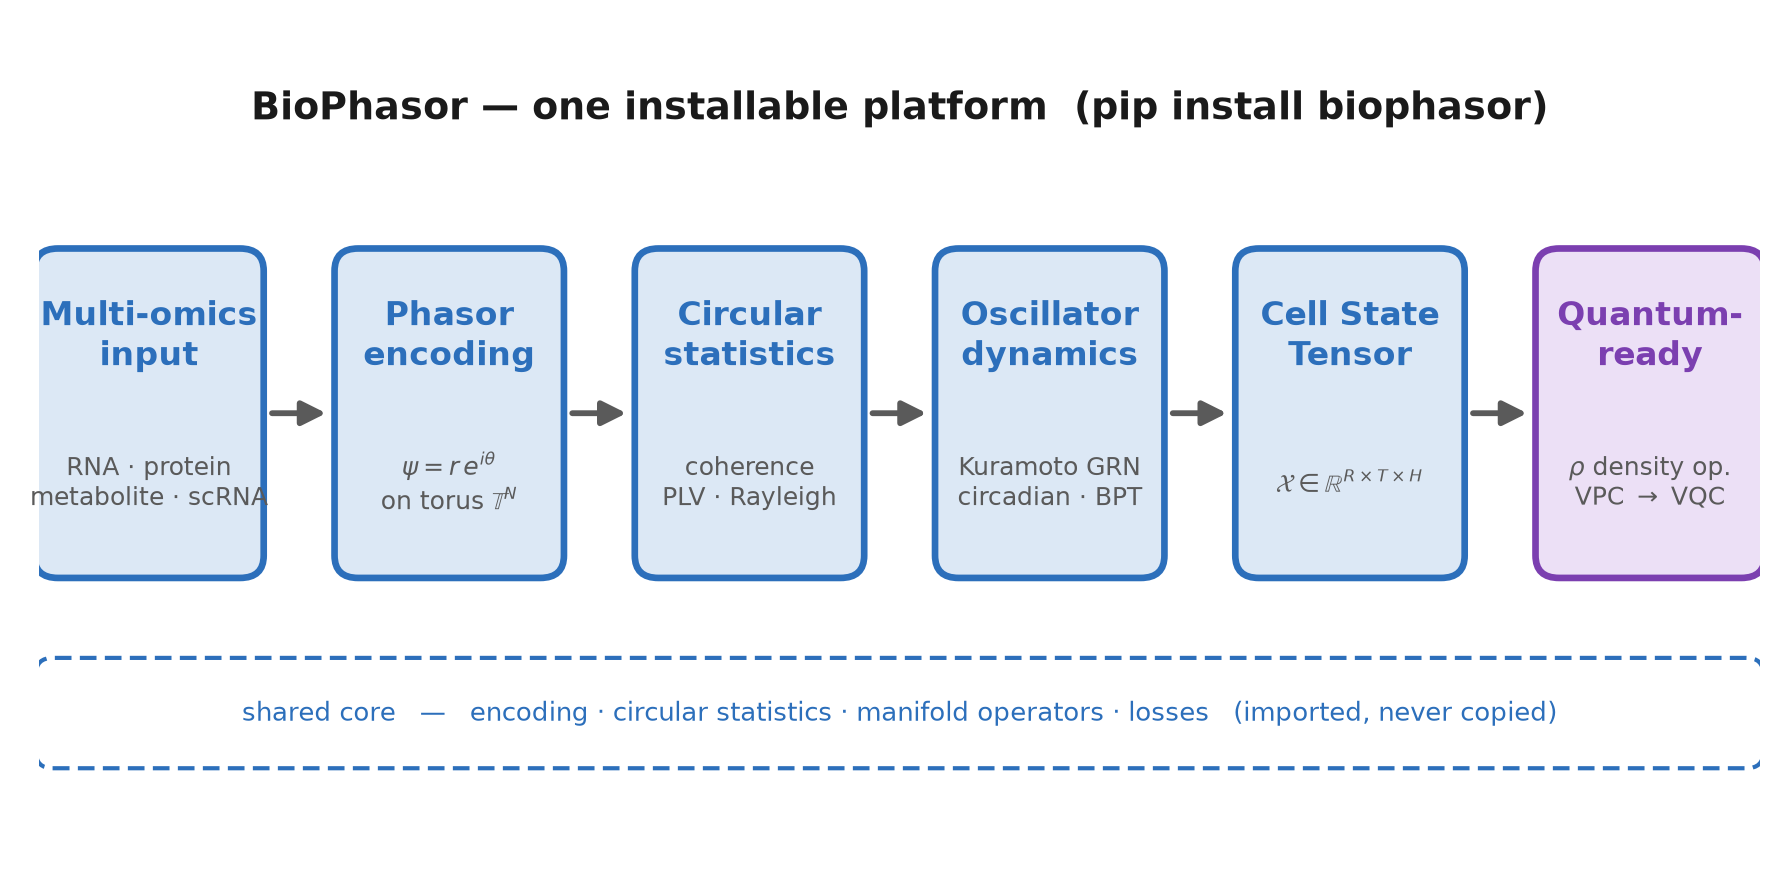
\includegraphics[width=\linewidth]{fig_platform_overview.png}
\caption{\textbf{The BioPhasor platform.} Multi-omics measurements are encoded as
complex phasors $\psi=r\,e^{i\theta}$ on the $N$-torus, then processed through a
common pipeline---circular statistics, coupled-oscillator dynamics, and the Cell
State Tensor---to a native quantum-information reading (the phase-coherence density
operator $\rho$ and the Variational Phasor Circuit, which transpiles to a
variational quantum circuit). A single shared \texttt{core} (encoding, circular
statistics, manifold operators, losses) is imported---never copied---by every
module, so one canonical implementation of each operation serves the whole
platform. Each stage is usable in isolation or as the full
encode~$\to$~filter~$\to$~fuse~$\to$~classify pipeline. BioPhasor is released as a
single installable package intended to host a series of use-case studies.}
\label{fig:platform_overview}
\end{figure*}

The advent of high-throughput sequencing has generated an unprecedented
multi-dimensional view of cellular state~\cite{ref_001,ref_003,ref_004,ref_005,ref_007}.
By simultaneously profiling the transcriptome (RNA-seq), epigenome (ATAC-seq),
proteome, and metabolome, researchers aim to reconstruct the hierarchical
regulatory networks governing biological life.
However, integrating these disparate data modalities remains a primary challenge
in computational biology~\cite{ref_010}.

\subsection{Motivation: From Clockwork Biology to Geometric Integration}

A recurring obstacle in multi-omics computation is scale heterogeneity:
the modalities operate on fundamentally different numerical ranges---RNA
counts ($\sim 10^4$) versus TF ChIP-seq ($\sim 10^0$) versus metabolite
concentrations ($\mu$M)---so that combining them requires aggressive
normalization. A second, more subtle obstacle is geometric: existing
integration methods (MOFA+, SNF, CCA, scVI) impose Euclidean structure on
data that is inherently circular, since biological states from mitosis to
circadian rhythms are closed oscillatory trajectories rather than linear
endpoints.

\textbf{BioPhasor} addresses both by representing each omic feature as a
phase angle $\phi \in (-\pi,\pi]$ on the unit circle and collecting the full
multi-omics state on the compact $N$-Torus $\mathbb{T}^N$.
This circular representation is simultaneously scale-invariant, topology-aware,
and compatible with well-developed circular statistics.

\subsubsection{The Legacy of Biological Oscillators}

The recognition that cellular life is a rhythmic process traces to early
circadian and ultradian oscillator
models~\cite{goodwin1965oscillatory,goldbeter1995model}.
These models captured the periodic ``clockwork'' of negative feedback
loops---the suprachiasmatic nucleus (SCN) and cell cycle---via coupled
differential equations.
Yet they were inherently low-dimensional, confined to manually curated
genes such as \textit{Period} (\textit{Per}) and
\textit{Cryptochrome} (\textit{Cry}).

\subsubsection{The Multi-Omics Expansion and the Euclidean Bottleneck}

With high-throughput sequencing, modeling shifted to \textbf{Euclidean deep
learning}~\cite{ref_031,ref_032,ref_033,ref_034,ref_035,ref_036,ref_037,ref_038,ref_039,ref_040}.
Variational Autoencoders~\cite{kingma2013auto} and
Transformers~\cite{vaswani2017attention} cluster cell types and predict
phenotypes effectively, but they treat gene expression as a linear magnitude
in $\reals^N$.
This abstraction introduces three fundamental errors for biological data:

\begin{enumerate}
    \item \textbf{Periodicity mismatch.}
    Biological states---from mitosis to metabolic pulses---are circular.
    In a linear model, the start and end of a cycle appear as antipodal
    points rather than adjacent states on a manifold.

    \item \textbf{Saturation blindness.}
    Biological signals saturate (Michaelis-Menten kinetics~\cite{michaelis1913die});
    once a promoter is occupied, additional concentration does not increase
    output. Euclidean activations require complex non-linear engineering to
    approximate this threshold behaviour.

    \item \textbf{Cross-omic scale heterogeneity.}
    Combining RNA counts with TF ChIP-seq peaks creates numerical instability,
    demanding aggressive normalization that destroys biologically meaningful signal.
\end{enumerate}

\subsubsection{Phase Dynamics: The Missing Link}

The most robust framework for periodic biological systems has long been
\textbf{phase dynamics}~\cite{ref_021,ref_022,ref_023,ref_027,ref_028,ref_030}.
EEG studies and circadian biology consistently show that the \emph{timing}
(phase) of a signal carries more regulatory information than its
\emph{amplitude}.
The ``Oscillatory Cell'' hypothesis underlies BioPhasor: every omic feature
is a phasor $e^{i\phi}$ rotating on a high-dimensional $N$-Torus $\torus^N$.

\subsubsection{BioPhasor: Scope and Contributions}

\begin{itemize}
    \item \textbf{Unified multi-omics phasor API.}
    A single library covers RNA-seq, scRNA-seq, proteomics, metabolomics,
    and multi-omics fusion with modality-aware encoding strategies.

    \item \textbf{Riemannian manifold operations.}
    Geodesic distance, Fr\'{e}chet mean, log/exp maps, and geodesic
    interpolation give topologically correct statistics on $\torus^N$,
    replacing ad hoc Euclidean approximations.

    \item \textbf{Oscillator dynamics.}
    The BioKuramoto model captures gene regulatory network synchrony as coupled
    phase oscillators; the circadian phasor module extracts phase, amplitude,
    and rhythmicity score via the Biological Phasor Transform (BPT).

    \item \textbf{Cell-state assignment.}
    The cell-cycle phasor module assigns G1/S/G2/M from marker gene phasors;
    the same approach supports custom state spaces (EMT, senescence, quiescence).

    \item \textbf{Phasor machine learning.}
    Variational Phasor Circuits (VPC), Phasor Transformers, and the Large
    Phasor Model (LPM) provide a full hierarchy of phase-native
    architectures with circular loss functions.

    \item \textbf{Dissipative dynamics and attractor landscape.}
    Cells are modelled as phase-coupled dissipative oscillators whose
    collective dynamics generate proliferating limit cycles.  The
    attractor geometry---topology, basin structure, and transition
    dynamics---is formalized via the Waddington quasi-potential and
    Floquet stability analysis (Section~\ref{sec:formulation}).

    \item \textbf{Cell State Tensor (CST).}
    An order-3 (three-way) tensor $\mathcal{X}_t \in \reals^{R \times T \times H}$
    encoding regulatory, temporal, and homeostatic cell state, derived
    from attractor-geometric features (global coherence, phase entropy,
    Floquet resilience, Markov transition entropy)---the canonical
    latent field summarizing the cell's attractor landscape
    (Section~\ref{sec:cst}). Its axes are rooted in \emph{measured}
    multi-omics quantities---a pathway/module atlas on the regulatory axis
    and an ordered central-dogma modality axis---rather than abstract
    categories (Section~\ref{subsec:cst_measured}).

    \item \textbf{A quantum-ready CST.}
    The CST's regulatory structure is carried by a phase-coherence density matrix
    $\rho$---a Hermitian, positive-semidefinite operator on the phasor field. We
    make the classical$\leftrightarrow$quantum correspondence of the CST explicit
    at the state level (von Neumann entropy and coherence of $\rho$) and the gate
    level (the Variational Phasor Circuit transpiles to a variational quantum
    circuit), establishing the structural sense in which decoding the CST is a
    quantum-ready computation (Section~\ref{sec:quantum_correspondence}); no
    empirical quantum advantage is claimed.

    \item \textbf{Open ecosystem.}
    Comprehensive documentation and validated experimental
    pipelines for research reproducibility.
\end{itemize}

By grounding BioPhasor in circadian oscillator theory, dissipative dynamics,
and the compact geometry of $\torus^N$, we provide a unified toolkit for
multi-omics analysis that treats regulatory timing, rather than expression
magnitude, as the primary signal.

\paragraph{What is specific to multi-omics.}
Phase-geometric state tensors have been proposed in other domains---most
directly for neural recordings, where a spatiotemporal tensor is indexed by
spectral band, anatomical region, and time. It would be easy to read the CST as
a transposition of that idea onto genes, and an earlier framing indeed defined
it largely by analogy. We take the opposite view: the value of a phasor state
tensor lies entirely in whether its axes are the measured, structured
quantities of \emph{its own} domain, and multi-omics offers two that have no
neural counterpart. First, the regulatory axis is organised by a
\emph{pathway/module atlas}: genes group into curated functional programs
(here the MSigDB Hallmark collection~\cite{ref_liberzon_hallmark}) exactly as
voxels group into anatomical regions, and we show
(Section~\ref{subsec:r_cst_pathway}) that this biological grouping---not the
analogy---is what makes the CST compressible and its factors interpretable.
Second, multi-omics has a directionally-\emph{ordered} axis with no analogue in
a spatial neural tensor: the central dogma
(DNA\,$\rightarrow$\,mRNA\,$\rightarrow$\,protein\,$\rightarrow$\,metabolite),
along which cross-modal phase coupling encodes post-transcriptional regulation
(Section~\ref{subsec:r_cst_pac}); whether that coupling itself flows
directionally is a separate question, and we find it symmetric at the cohort
level. These two properties---a biological atlas for the regulatory axis and an
intrinsically-ordered modality axis---are what root BioPhasor in the structure
of multi-omics data rather than in a borrowed template.

\paragraph{Scope of this paper.}
This is a \emph{platform and method} paper. Our aim is to establish the BioPhasor
formulation---the phasor encoding, its circular and Riemannian statistics, the
coupled-oscillator dynamics, the Cell State Tensor, and the
classical$\leftrightarrow$quantum correspondence (Fig.~\ref{fig:platform_overview})---and
to release it as a single, reproducible software ecosystem. Accordingly the empirical results below are
\emph{illustrative capability demonstrations}: nine end-to-end vignettes on real
public data that show each component works as claimed and map where a
phase-geometric view helps and where it does not. They are not a single headline
study. Individual findings that merit a full treatment---most notably the
tumour-specific cross-modal coupling along the central dogma
(Section~\ref{subsec:r_cst_pac})---are developed as standalone use-case studies
elsewhere; here they exercise the platform. We intend BioPhasor to host a series
of such use-case manuscripts, each building on the shared formulation and code
rather than re-deriving it.

We are also explicit about what this paper is \emph{not}. BioPhasor is a data
engineering and modelling framework for multi-omics phase geometry; it is not a
clinical or diagnostic tool. We make no diagnostic, prognostic, or therapeutic
claim: the platform does not diagnose disease, stratify patients, or prescribe
treatment. The clinical and therapeutic directions we discuss---phase-based
detection of drug-resistant sub-populations, a ``cellular digital twin'' for
state monitoring, and \emph{attractor therapy} for guided cell-state
reprogramming---are stated deliberately as \emph{prospective applications the
platform could enable}, motivating future work; each would require dedicated
study, validation on appropriately powered clinical cohorts, and regulatory
evaluation before any use. Nothing here is validated for clinical use.
% --- END sections/introduction.tex ---

% --- BEGIN sections/related_work.tex (inserted in revision) ---
\section{Related Work}
\label{sec:related_work}

BioPhasor sits at the intersection of three established lines of work---phase
representations of gene expression, coupled-oscillator models of regulatory
networks, and multi-omics integration---and it is important to state plainly
which of its components extend prior art and which re-implement it.

\paragraph{Phase and oscillatory representations of gene expression.}
Encoding genes as phases and analysing their synchrony is not new. Kim et al.~\citep{kim2008bmc}
introduced a phase-synchronization clustering algorithm that maps cell-cycle
expression onto phase angles and groups genes by phase coherence, and related
self-organizing-map work formalised statistical phase synchronization of
expression the same year \citep{kim2008somps}. More recently, Wang et al.~\citep{wang2025} proposed a four
eigen-phase decomposition of \emph{multi-omics} data on the yeast metabolic
cycle, and Bardozzo et al.~\citep{bardozzo2020} analysed oscillatory patterns across bacterial
multi-omic layers with explicit signal metrics. BioPhasor's tanh-phase encoding,
phase-coherence statistic, and Biological Phasor Transform are therefore a
generalization of an established idea rather than a new one; our contribution on
this axis is not the phasor encoding per se but its extension to arbitrary
patient cohorts and to an ordered central-dogma modality axis
(Section~\ref{subsec:r_cst_pac}).

\paragraph{Coupled-oscillator models of regulatory networks.}
The Kuramoto model has a long history in biology, from circadian pacemaker
synchronization to network-topology studies. Selvarajoo~\citep{selvarajoo2019} showed that
large scale-free and small-world biological networks reach synchronization at
lower coupling than homogeneous graphs---precisely the hub-lowers-threshold
phenomenology our BioKuramoto experiment recovers
(Section~\ref{subsec:r_kuramoto}). We therefore present the critical-coupling
and topology-dependence results as a \emph{validation that the implementation
reproduces known Kuramoto behaviour on real co-expression coupling}, not as a
discovery.

\paragraph{Multi-omics integration.}
The dominant integration frameworks are Euclidean-latent-factor and
network-fusion methods. Multi-Omics Factor Analysis \citep{argelaguet2018} and
its successor MOFA+ \citep{argelaguet2020} learn shared latent factors across
modalities; MEFISTO \citep{velten2022} extends this with smooth temporal and
spatial factors and is the closest methodological competitor to a phase-native
approach on time-structured data; Similarity Network Fusion \citep{wang2014}
fuses per-modality sample-similarity graphs; and probabilistic single-cell
models---scVI \citep{lopez2018}, totalVI \citep{gayoso2021}, and the
scANVI/empirical-Bayes line \citep{xu2021,boyeau2023}---provide
distribution-aware integration for count and multimodal data. We benchmark
BioPhasor head-to-head against MOFA+/MEFISTO and SNF on an identical matched
matrix (Section~\ref{subsec:r_multiomics}) rather than only contrasting design
philosophies. A separate line represents multi-omics \emph{circularly} for
convolutional models---OmicsFootPrint \citep{njoku2024} renders samples as
circular images---which we distinguish from BioPhasor's use of the circle as
the state space of a phase variable rather than as a display substrate.

\paragraph{Circadian rhythmicity detection and phase-amplitude coupling.}
Rhythmicity calling from transcriptomic time series is a mature area: MetaCycle
\citep{wu2016} integrates JTK\_CYCLE-style periodicity tests, and likelihood- and
model-based callers \citep{braun2018,ding2021,rubioponce2021} set the standard
against which our CircadianPhasor rhythmicity scores should be measured. Our
central-dogma coupling analysis (``Omics-PAC'') borrows the modulation-index
machinery of cross-frequency phase-amplitude coupling from neuroscience
\citep{scherer2022}; the novel step is transposing it from two frequency bands
of one signal onto two \emph{modalities} along the ordered central-dogma axis,
relating mRNA phase and protein amplitude---a coupling with no neural
counterpart, motivated biologically by widespread post-transcriptional
regulation \citep{srivastava2022}. Whether the coupling is directional is tested
separately (Section~\ref{subsec:r_cst_pac}) and found symmetric at the cohort
level.

\paragraph{Attractor landscapes and pathway priors.}
Finally, the dissipative/attractor formulation (Section~\ref{sec:formulation})
builds on deterministic quasi-potential constructions of Waddington's landscape
\citep{bhattacharya2011}, and the pathway-atlas that roots the CST regulatory
axis uses the MSigDB Hallmark collection \citep{liberzon2015}, with cell-cycle
phase assignment referenced to the canonical S/G2M marker sets \citep{tirosh2016}.
These are used as established tools, not presented as contributions.

\paragraph{What is new.}
Against this backdrop the defensible contributions of BioPhasor are three:
(i)~a \emph{cross-modality} phase-amplitude coupling along the central-dogma
axis, measured with a proper surrogate null and shown to be tumour-specific
and---at the cohort level---symmetric rather than directional
(Section~\ref{subsec:r_cst_pac}); (ii)~a single, reproducible
software ecosystem that unifies phasor encoding, circular statistics,
coupled-oscillator dynamics, the Cell State Tensor, and an explicit
classical$\leftrightarrow$quantum correspondence behind one data layer; and
(iii)~an honest cross-cohort scoping of \emph{where} a phase-geometric view adds
information (repeated-sampling, low-dropout modalities) and where it does not
(sparse single-cell selection, naive coherence-averaged fusion).
% --- END sections/related_work.tex ---


% --- BEGIN sections/theory.tex ---
% theory.tex
\section{Theory: Phasor Dynamics on the $N$-Torus}
\label{sec:theory}

This section establishes the mathematical framework underlying the
BioPhasor framework.
We present: (1) the $N$-Torus state space and phasor encoding;
(2) circular statistics and coherence theory;
(3) the Riemannian manifold geometry of $\torus^N$;
(4) coupled oscillator dynamics (Kuramoto); and
(5) the Biological Phasor Transform for time-series analysis.

% ----------------------------------------------------------------
\subsection{State Space: The $N$-Torus and Phasor Encoding}
\label{subsec:state_space}

In traditional bioinformatics, a cell's regulatory state is modeled as
$\boldsymbol{x} \in \reals^N$~\cite{ref_051,ref_052,ref_053,ref_054,ref_055},
where each component carries arbitrary magnitude noise.
BioPhasor instead defines the state space for $N$ omic features as the
continuous $N$-Torus:
\begin{equation}
    \torus^N = \underbrace{S^1 \times S^1 \times \cdots \times S^1}_{N}.
\end{equation}
Each cell's multi-omic state is represented as a complex phasor vector:
\begin{equation}
    \boldsymbol{z} = \begin{pmatrix} z_1 \\ \vdots \\ z_N \end{pmatrix}
    = \begin{pmatrix} e^{i\phi_1} \\ \vdots \\ e^{i\phi_N} \end{pmatrix}
    \in \complex^N, \quad |z_k| = 1 \;\forall\; k.
\end{equation}

\begin{definition}[Omic Phasor Encoding]
\label{def:encoding}
Given a normalized feature value $x_j$ (e.g., CPM-normalized RNA count),
define the tanh-phase encoding map:
\begin{equation}
    \phi_j = \pi \cdot \tanh\!\left(\frac{\log_{1p}(x_j) - \mu_j}
    {\sigma_j + \varepsilon}\right),
    \qquad z_j = e^{i\phi_j} \in S^1,
\end{equation}
where $\mu_j$, $\sigma_j$ are gene-wise mean and standard deviation, and
$\varepsilon > 0$ ensures numerical stability.
By construction, $\phi_j \in (-\pi, \pi)$.
For methylation $\beta$-values (log-linear encoding) and log2-scaled
proteomics (linear encoding), modality-specific mappings are applied
(Section~\ref{subsec:biophasor_encoding}).
\end{definition}

This geometric embedding provides two key biological invariances:
\begin{itemize}
    \item \textbf{Scale invariance}: phase is immune to multiplicative
    magnitude scaling (sequencing depth, batch effects).
    \item \textbf{Manifold compactness}: $\torus^N$ is bounded, eliminating
    exploding gradients in deep architectures.
\end{itemize}

Figure~\ref{fig:omic_encoding} illustrates the encoding pipeline.

\begin{figure}[!htb]
\centering
\resizebox{\textwidth}{!}{% --- BEGIN figures/fig_omic_encoding.tex ---
% fig_omic_encoding.tex — Phasor encoding pipeline for omics
% Pipeline: raw → log → z-score → tanh → S^1 phasor   +   unit circle right panel
% All colors hardcoded. No parameterised TikZ style colour args.

\colorlet{encRaw}{colNeutral!12!white}
\colorlet{encLog}{colChrom!14!white}
\colorlet{encZsc}{colTF!14!white}
\colorlet{encTnh}{colEpi!14!white}
\colorlet{encPhs}{colRNA!14!white}

\begin{tikzpicture}[>=Latex, font=\small]

%% Pipeline boxes (spaced 4.2 cm apart)
\node[rectangle, rounded corners=6pt, minimum width=3.2cm, minimum height=1.8cm,
      align=center, text width=3.0cm, inner sep=9pt,
      fill=encRaw, draw=colNeutral, line width=1.4pt]
  (raw) at (0,0) {\textbf{Raw Count}\\[5pt] $x_j \in \reals_{\geq 0}$};

\node[rectangle, rounded corners=6pt, minimum width=3.2cm, minimum height=1.8cm,
      align=center, text width=3.0cm, inner sep=9pt,
      fill=encLog, draw=colChrom, line width=1.4pt]
  (logn) at (4.2,0) {\textbf{Log Norm}\\[5pt] $x_j' = \log(x_j{+}1)$};

\node[rectangle, rounded corners=6pt, minimum width=3.2cm, minimum height=1.8cm,
      align=center, text width=3.0cm, inner sep=9pt,
      fill=encZsc, draw=colTF, line width=1.4pt]
  (zsc) at (8.4,0) {\textbf{Z-score}\\[5pt] $\hat{x}_j = \tfrac{x_j'-\mu}{\sigma+\varepsilon}$};

\node[rectangle, rounded corners=6pt, minimum width=3.2cm, minimum height=1.8cm,
      align=center, text width=3.0cm, inner sep=9pt,
      fill=encTnh, draw=colEpi, line width=1.4pt]
  (tanh) at (12.6,0) {\textbf{Tanh Map}\\[5pt] $\theta_j=\pi\tanh(\hat{x}_j)$};

\node[rectangle, rounded corners=6pt, minimum width=3.2cm, minimum height=1.8cm,
      align=center, text width=3.0cm, inner sep=9pt,
      fill=encPhs, draw=colRNA, line width=1.4pt]
  (phs) at (16.8,0) {\textbf{Phasor}\\[5pt] $z_j = e^{i\theta_j}\!\in\!S^1$};

%% Arrows
\draw[->, line width=1.8pt, color=colNeutral, shorten >=4pt, shorten <=4pt]
  (1.6,0) -- node[above, font=\scriptsize, yshift=2pt] {depth norm} (2.6,0);
\draw[->, line width=1.8pt, color=colChrom,  shorten >=4pt, shorten <=4pt]
  (5.8,0) -- node[above, font=\scriptsize, yshift=2pt] {standardize} (6.8,0);
\draw[->, line width=1.8pt, color=colTF,     shorten >=4pt, shorten <=4pt]
  (10.0,0) -- node[above, font=\scriptsize, yshift=2pt] {saturate} (11.0,0);
\draw[->, line width=1.8pt, color=colEpi,    shorten >=4pt, shorten <=4pt]
  (14.2,0) -- node[above, font=\scriptsize, yshift=2pt] {lift to $S^1$} (15.2,0);

%% Sub-labels
\foreach \bx/\tx in {
  0/{$x_j\in[0,10^5]$},
  4.2/{$x_j'\in[0,12]$},
  8.4/{$\hat x_j\in\reals$},
  12.6/{$\theta_j\in(-\pi,\pi)$},
  16.8/{$|z_j|=1$}
}{
  \node[font=\footnotesize\itshape, color=colNeutral] at (\bx,-1.45) {\tx};
}

%% Unit circle right panel
\begin{scope}[shift={(23.5,0)}]
  \draw[gray!30, line width=0.8pt] (0,0) circle(2.0);
  \draw[->, gray!45, line width=0.5pt] (-2.6,0)--(2.6,0)
    node[right, font=\tiny, gray] {Re};
  \draw[->, gray!45, line width=0.5pt] (0,-2.6)--(0,2.6)
    node[above, font=\tiny, gray] {Im};

  % Five phasors
  \foreach \ang/\col/\lbl in {
    30/colRNA/mRNA,
    75/colChrom/Chromatin,
    130/colEpi/Methylation,
    200/colTF/TF-Binding,
    310/colNeutral/Protein
  }{
    \draw[->, color=\col, line width=2.0pt]
      (0,0) -- ({1.90*cos(\ang)},{1.90*sin(\ang)});
    \node[color=\col, font=\footnotesize\bfseries]
      at ({2.45*cos(\ang)},{2.45*sin(\ang)}) {\lbl};
  }
  % Mean phasor
  \draw[->, black!75, line width=2.4pt, dashed]
    (0,0) -- ({1.0*cos(105)},{1.0*sin(105)})
    node[left, font=\scriptsize\bfseries, xshift=-2pt] {$\bar{z}$};
  % Coherence label
  \node[font=\small\bfseries, color=colCoher, align=center] at (0,-3.0)
    {$\coherence = |\bar{z}|$};
\end{scope}

%% Linking arrow to circle
\draw[->, line width=1.8pt, color=colRNA, shorten >=6pt, shorten <=4pt]
  (18.4,0) -- node[above, font=\scriptsize, yshift=2pt] {5 omics} (21.5,0);

\end{tikzpicture}
% --- END figures/fig_omic_encoding.tex ---
}
\caption{\textbf{BioPhasor Omic Phasor Encoding Pipeline.}
Raw counts are CPM-normalized, log-transformed, z-scored, then compressed
to $(-\pi,\pi)$ via $\tanh$ and lifted to $S^1$ via $e^{i\phi}$.
\textit{Right}: Five example phasors from transcriptomics
(\textcolor{colRNA}{red}), epigenomics (\textcolor{colEpi}{purple}),
chromatin (\textcolor{colChrom}{green}), TF binding (\textcolor{colTF}{blue}),
and their circular mean $\bar{z}$ (dashed).}
\label{fig:omic_encoding}
\end{figure}

% ----------------------------------------------------------------
\subsection{BioPhasor Encoding Strategies}
\label{subsec:biophasor_encoding}

Different omics modalities have distinct distributional characteristics
requiring tailored encoding maps.
BioPhasor implements three strategies:

\paragraph{Tanh-Phase Encoding (RNA-seq, ATAC-seq).}
For right-skewed count data, the canonical encoding applies log1p
transformation followed by per-gene z-scoring and tanh saturation:
\begin{equation}
    \phi_j^{\mathrm{tanh}} = \pi \cdot
    \tanh\!\left(\frac{\log_{1p}(x_j) - \mu_j}{\sigma_j}\right).
\end{equation}
Among the three encoders this achieves the widest phase spread
($\sigma_\phi \approx 1.995$ radians), which maximizes the angular
resolution available to the downstream coherence statistics.

\paragraph{Log-Linear Encoding (DNA Methylation $\beta$-values).}
Methylation $\beta \in [0,1]$ maps linearly to $(-\pi,\pi)$ via the logit:
\begin{equation}
    \phi_j^{\mathrm{log}} = \pi \cdot
    \mathrm{clip}\!\left(\frac{\log(\beta_j) - x_{\min}}{x_{\max} - x_{\min}}
    \cdot 2 - 1,\,-1,\,1\right).
\end{equation}

\paragraph{Linear Encoding (Proteomics, log2-scaled).}
For approximately symmetric log2-transformed data:
\begin{equation}
    \phi_j^{\mathrm{lin}} = \pi \cdot
    \left(\frac{2(x_j - x_{\min})}{x_{\max} - x_{\min}} - 1\right).
\end{equation}

\noindent
The auto-dispatch encoder selects the correct
strategy based on modality name:


% ----------------------------------------------------------------
\subsection{Circular Statistics of Phasor Distributions}
\label{subsec:circular_stats}

\begin{definition}[Phase Coherence (Mean Resultant Length)]
\label{def:coherence}
For $N$ phasors $\{e^{i\phi_k}\}_{k=1}^N$, the phase coherence is:
\begin{equation}
    \mathcal{C} = \frac{1}{N}\left|\sum_{k=1}^N e^{i\phi_k}\right| \in [0,1].
\end{equation}
$\mathcal{C} = 1$ iff all phasors are co-aligned;
$\mathcal{C} \approx 0$ under uniformly random phases.
\end{definition}

\begin{theorem}[Coherence as a Systems-Order Biomarker]
\label{thm:coherence}
The scalar $\mathcal{C}$ monotonically increases with the alignment of
phasors on $S^1$. In multi-omics, $\mathcal{C}$ quantifies the
synchronization of regulatory programs across genes or samples.
\end{theorem}

\begin{corollary}[Disease-State Stratification via Coherence]
\label{cor:disease}
The framework predicts that phase coherence $\bar{\mathcal{C}}$ stratifies
disease states differing in regulatory coordination: e.g.\ quiescent
IGHV-mutated versus autonomously-signaling IGHV-unmutated CLL are expected to
separate by mean coherence, reflecting their distinct BCR-signaling
phenotypes. This is a testable prediction to be evaluated on labelled real
cohorts (Section~\ref{subsec:r_ml}, Section~\ref{subsec:data_sources}).
\end{corollary}

\paragraph{Rayleigh Test for Phase Uniformity.}
A gene is declared \emph{phase-coherent} if the Rayleigh test rejects
the null hypothesis of uniform phase distribution:
\begin{equation}
    W = 2N\mathcal{C}^2, \qquad W \overset{H_0}{\sim} \chi^2_2
    \quad (\text{large sample}), \qquad p = e^{-W/2}.
\end{equation}
BioPhasor implements this test.

\paragraph{Fr\'{e}chet Mean (Circular Mean).}
The unbiased circular mean of phasors $\{\phi_k\}$ is:
\begin{equation}
    \bar{\phi}_F = \arg\left(\sum_{k=1}^N e^{i\phi_k}\right)
    = \mathrm{atan2}\!\left(\sum\sin\phi_k,\, \sum\cos\phi_k\right).
\end{equation}
This Fr\'{e}chet mean replaces the arithmetic mean wherever phase data are circularly distributed.

% ----------------------------------------------------------------
\subsection{Riemannian Geometry of $\torus^N$}
\label{subsec:manifold}

\begin{definition}[Geodesic Distance on $\torus^N$]
\label{def:geodesic}
The geodesic distance between two phasors $\phi_1, \phi_2 \in S^1$ is
the arc-length:
\begin{equation}
    d(\phi_1, \phi_2) =
    |\mathrm{atan2}(\sin(\phi_1 - \phi_2),\cos(\phi_1 - \phi_2))| \in [0,\pi].
\end{equation}
For $N$-dimensional phasor vectors:
\begin{equation}
    d(\boldsymbol{\phi}_s, \boldsymbol{\phi}_r) = \sqrt{\frac{1}{N}
    \sum_{g=1}^N d(\phi_{sg},\,\phi_{rg})^2}.
\end{equation}
\end{definition}

\paragraph{Log/Exp Maps for Tangent-Space Analysis.}
The log map projects $\torus^N$ to the flat Euclidean tangent space at a
base point $\boldsymbol{\mu}$, enabling unbiased linear operations (PCA, regression):
\begin{equation}
    \mathrm{Log}_{\boldsymbol{\mu}}(\boldsymbol{\phi}) =
    \mathrm{wrap}(\boldsymbol{\phi} - \boldsymbol{\mu}), \qquad
    \mathrm{Exp}_{\boldsymbol{\mu}}(\boldsymbol{v}) =
    \mathrm{wrap}(\boldsymbol{\mu} + \boldsymbol{v}).
\end{equation}
These are exact inverses on $\torus^N$ (no approximation needed).

\paragraph{Geodesic Interpolation (Phasor Pseudo-Time).}
For samples $\boldsymbol{\phi}_A$ and $\boldsymbol{\phi}_B$
(e.g., starting and terminal cell states), the geodesic trajectory
parameterized by $t \in [0,1]$ is:
\begin{equation}
    \boldsymbol{\phi}(t) = \mathrm{Exp}_{\boldsymbol{\phi}_A}
    \!\bigl(t \cdot \mathrm{Log}_{\boldsymbol{\phi}_A}
    (\boldsymbol{\phi}_B)\bigr) = \mathrm{wrap}
    (\boldsymbol{\phi}_A + t \cdot \mathrm{wrap}
    (\boldsymbol{\phi}_B - \boldsymbol{\phi}_A)).
\end{equation}
This provides a parameter-free pseudo-time for single-cell trajectories.

% ----------------------------------------------------------------
\subsection{Unitary Operations: Regulatory Interference}
\label{subsec:unitary}

Once cell states are encoded on $\torus^N$, regulatory interactions are
modeled by unitary operators:
\begin{equation}
    \mathcal{U}(1) = \bigl\{e^{i\theta} \mid \theta \in [0,2\pi)\bigr\}.
\end{equation}

\begin{definition}[Cross-Layer Interference Matrix]
\label{def:interference}
For $\boldsymbol{\phi} \in \torus^N$, the pairwise regulatory interaction
matrix $I \in [-1,+1]^{N \times N}$ is:
\begin{equation}
    [I]_{jk} = \cos(\phi_j - \phi_k) = \mathrm{Re}(z_j\bar{z}_k).
\end{equation}
$I_{jk} = +1$ implies co-activation; $I_{jk} = -1$ implies mutual repression;
$I_{jk} \approx 0$ indicates orthogonal independence.
\end{definition}

The pull-back operator restores manifold compactness after linear mixing:
\begin{equation}
    \mathcal{P}(z) = \frac{z}{|z| + \varepsilon} \longrightarrow e^{i\arg(z)}.
\end{equation}

% ----------------------------------------------------------------
\subsection{Variational Phasor Circuit (VPC)}
\label{subsec:vpc}

The VPC implements
biological regulation via two gate types:
\begin{enumerate}
    \item \textbf{Parameterized Shift Gates}: learnable phase rotations
    $S_k(\theta_k) = \mathrm{diag}(1,\ldots,e^{i\theta_k},\ldots,1)$.
    \item \textbf{Entangling Mix Gates}: 50:50 beam-splitter
    $M = \frac{1}{\sqrt{2}}\begin{pmatrix}1 & i\\i&1\end{pmatrix}$
    modelling pairwise omic cross-talk.
\end{enumerate}
A single VPC layer: $\boldsymbol{z}_{t+1} = \mathcal{P}(M\,S(\boldsymbol{\theta})\,\boldsymbol{z}_t)$.
Parameter scaling: $\mathcal{O}(LN)$ for depth $L$ and width $N$,
vs.\ $\mathcal{O}(N^2)$ for dense Euclidean layers.

% ----------------------------------------------------------------
\subsection{Quantum Parallel: VPC as a Classically-Simulated VQC}
\label{subsec:vpc_vqc}

Because the VPC acts on unit-modulus phasors through phase rotations and
norm-preserving mixing, its gate algebra maps one-to-one onto a Variational
Quantum Circuit (VQC)~\cite{cerezo2021variational,benedetti2019parameterized}.
Each parameterized shift $S_k(\theta_k)=\mathrm{diag}(1,\dots,e^{i\theta_k},
\dots,1)$ becomes a single-qubit $R_z(\theta_k)$ rotation; the entangling Mix
gate becomes a CNOT$+R_z$ entangling layer; and the DFT token-mixing block
becomes a Quantum Fourier Transform (QFT). The VPC therefore operates on the
phase-diagonal sector of an $N$-qubit Hilbert space, and its trained parameters
are directly usable as quantum rotation angles without reparametrization---the
multi-omics analogue of the correspondence established for phasor circuits in
neural signals. Table~\ref{tab:cst_quantum_correspondence} lists the gate
mapping; Section~\ref{sec:quantum_validation} evaluates it and its complexity
consequences on real multi-omics data.

\begin{table}[ht]
\centering\small
\caption{Gate-level correspondence between the classical Variational Phasor
Circuit and a Variational Quantum Circuit. The mapping is exact on the
phase-diagonal sector; complexity columns give per-operation asymptotic cost in
system size $N$ (number of gene/pathway phasors, i.e.\ qubits).}
\label{tab:cst_quantum_correspondence}
\begin{tabular}{p{3.6cm}p{3.6cm}p{4.4cm}}
\toprule
Classical VPC gate & Quantum VQC gate & Complexity (classical $\to$ quantum) \\
\midrule
Phasor $z=e^{i\theta}\in S^1$ & Qubit $|\psi\rangle$ on Bloch $S^2$
  & $S^1\subset S^2$ (equatorial slice) \\
Shift $S(\theta)$ & $R_z(\theta)$ rotation
  & $\mathcal{O}(1)\to\mathcal{O}(1)$ \\
Mix (beam-splitter) & CNOT$+R_z$ entangling layer
  & $\mathcal{O}(N)\to\mathcal{O}(N)$ \\
DFT token mixing & Quantum Fourier Transform
  & $\mathcal{O}(N\log N)\to\mathcal{O}((\log N)^2)$ \\
PLV matrix & Reduced density matrix $\rho_{jk}$
  & $\mathrm{PLV}=2|\rho_{jk}|$ (phase-diagonal) \\
\bottomrule
\end{tabular}
\end{table}

% ----------------------------------------------------------------
\subsection{Coupled Oscillator Dynamics: Kuramoto Model}
\label{subsec:kuramoto}

Gene regulatory networks are modeled as coupled phase oscillators via the
Kuramoto model:
\begin{equation}
    \frac{d\phi_i}{dt} = \omega_i + \frac{K}{N}\sum_{j=1}^N
    A_{ij}\sin(\phi_j - \phi_i) + \eta_i(t),
\end{equation}
where $\omega_i$ is the natural oscillation frequency of gene $i$,
$K$ is global coupling strength, $A_{ij}$ is the GRN adjacency matrix,
and $\eta_i(t) \sim \mathcal{N}(0, \sigma^2)$ is Gaussian noise.

The order parameter $R = |\frac{1}{N}\sum_j e^{i\phi_j}|$ measures
network-wide synchrony.
A phase transition occurs at critical coupling:
\begin{equation}
    K_c = \frac{2}{\pi g(\omega_0)},
\end{equation}
where $g(\omega_0)$ is the frequency distribution at the mean.
BioPhasor maps $(K,\sigma)$ parameter space to $R_\infty$,
quantifying synchrony robustness in realistic GRN topologies
(hub-spoke, scale-free).

% ----------------------------------------------------------------
\subsection{Biological Phasor Transform (BPT) for Time-Series}
\label{subsec:bpt}

For oscillatory time-series (circadian, cell cycle), the BPT extracts
phase and amplitude at biological frequencies via a single DFT:
\begin{equation}
    G + iS = \frac{1}{T}\sum_{k=0}^{T-1} I_k \cdot e^{-2\pi i k/(f\cdot T\cdot\Delta t)},
\end{equation}
where $f$ is the fundamental frequency (e.g., $f = 1/24$\,h for circadian).
Phase $\phi = \mathrm{atan2}(S,G)$ and amplitude $A = \sqrt{G^2+S^2}$
are extracted per gene, with the rhythmicity score $A/A_{\max}$ used
for gene calling.

ZT (Zeitgeber Time) maps directly to BPT phase:
\begin{equation}
    \mathrm{ZT} = \frac{(\phi+\pi)\cdot T}{2\pi}, \qquad
    \phi = \frac{2\pi\cdot\mathrm{ZT}}{T} - \pi.
\end{equation}
Implemented via single-frequency DFT extraction.

% ----------------------------------------------------------------
\subsection{Phase Locking Value and Synchrony Metrics}
\label{subsec:plv}

The Phase Locking Value (PLV) between genes $i$ and $j$ across $N$ samples:
\begin{equation}
    \mathrm{PLV}_{ij} = \frac{1}{N}\left|\sum_{n=1}^N
    e^{i(\phi_{ni} - \phi_{nj})}\right| \in [0,1].
\end{equation}
$\mathrm{PLV}_{ij} = 1$ indicates perfect phase locking (co-regulated);
$\mathrm{PLV}_{ij} = 0$ indicates independent expression.
The PLV matrix is used for module detection, hub gene identification, and batch correction.

\paragraph{Phase Lag Index (PLI).}
The PLI removes volume-conduction artefacts by sign-weighting:
\begin{equation}
    \mathrm{PLI}_{ij} = \left|\frac{1}{N}\sum_n
    \mathrm{sign}\!\bigl(\sin(\phi_{ni}-\phi_{nj})\bigr)\right|.
\end{equation}
PLI is zero for purely in-phase or anti-phase relationships and is
robust to common-source contamination in multi-omics batch effects.

% ----------------------------------------------------------------
\subsection{Multi-Omics Coherence Fusion}
\label{subsec:fusion}

For $M$ omics layers with per-sample phasors
$\{\boldsymbol{z}^{(m)}\}_{m=1}^M$, the weighted circular mean fusion is:
\begin{equation}
    \boldsymbol{z}_{\mathrm{fused}} = \arg\!\left(
    \sum_{m=1}^M \alpha_m \boldsymbol{z}^{(m)}\right), \qquad
    \alpha_m \geq 0,\; \sum_m \alpha_m = 1.
\end{equation}
The cross-layer coherence between modalities $m_1$ and $m_2$ is:
\begin{equation}
    C(m_1, m_2) = \left|\frac{1}{NF}\sum_{n,f}
    z_{nf}^{(m_1)}\overline{z_{nf}^{(m_2)}}\right| \in [0,1].
\end{equation}
Coherence-weighted fusion automatically up-weights layers with higher
internal coherence.

% ----------------------------------------------------------------
\subsection{Phasor Transformer and Large Phasor Model (LPM)}
\label{subsec:lpm}

For temporal multi-omics sequences (time-course RNA-seq, live-cell
imaging), a Phasor Transformer encodes long-range regulatory context:
\begin{equation}
    \mathbf{u}_t = \mathcal{T}_{\Theta_{\mathrm{PT}}}(\mathbf{x}_{1:t}),
\end{equation}
where frequency-domain token mixing replaces pairwise attention,
yielding $\mathcal{O}(T\log T)$ complexity for sequence length $T$.
The Large Phasor Model (LPM) combines transformer context with
high-capacity VPC modules:
\begin{equation}
    \boldsymbol{z}_t^{\mathrm{LPM}} =
    \mathcal{V}_{\Theta_{\mathrm{LVPC}}}(\mathbf{x}_t, \mathbf{u}_t).
\end{equation}
LPM is the core representational backbone: transformer layers capture
temporal regulatory dependencies (e.g., cell-cycle progression, circadian
entrainment), while large VPC layers perform geometric compression and
task-facing phase abstraction.

% ----------------------------------------------------------------
\subsection{Dissipative Oscillators and Phase Reduction}
\label{subsec:dissipative}

The cell is a far-from-equilibrium dissipative system: it imports free
energy and exports entropy at rates sufficient to sustain self-organised
oscillations~\cite{ref_prigogine1977}.  Each oscillatory subsystem---circadian
clock, cell-cycle, NF-$\kappa$B signalling---is modelled as a dissipative
oscillator that, under sufficient nonlinearity, undergoes a
\textbf{Hopf bifurcation} producing a stable limit cycle.

For a Goodwin-type regulatory circuit with Hill coefficient $n$, the
Hopf criterion determines the critical cooperativity:
\begin{equation}
    n > n_c \implies \text{stable limit cycle with period }
    \tau \approx \frac{2\pi}{\omega_0},
    \label{eq:hopf}
\end{equation}
where $\omega_0$ depends on degradation rates and binding constants.
Phase reduction then maps the full-dimensional dynamics onto $S^1$:
\begin{equation}
    \dot{\phi}_j = \omega_j
    + \sum_{k \neq j} W_{jk}\,H_{jk}(\phi_j - \phi_k),
    \label{eq:phase_reduction}
\end{equation}
the generalized Kuramoto model with asymmetric, frequency-dependent
coupling, which serves as the governing equation for phase dynamics
throughout the BioPhasor framework.

% ----------------------------------------------------------------
\subsection{Bifurcations and Cell-Fate Decisions}
\label{subsec:bifurcations}

Cell-fate decisions are modelled as bifurcations in the CST dynamical
system:
\begin{itemize}
    \item \textbf{Saddle-node} ($\dot\phi = \mu - \phi^2$): irreversible
    commitment (terminal differentiation).
    \item \textbf{Pitchfork} ($\dot\phi = \mu\phi - \phi^3$): symmetric
    binary fate choice (e.g., Th1/Th2 polarization).
    \item \textbf{Hopf}: stable limit cycle from fixed point---oscillatory
    stem-cell maintenance where pluripotency requires sustained
    oscillation of Nanog, Hes1, and Dll1~\cite{ref_imayoshi2013}.
\end{itemize}
% --- END sections/theory.tex ---

% --- BEGIN sections/formulation.tex ---
% formulation.tex — Biophasor Formulation: Dissipative Dynamics and CST Pipeline
\section{Biophasor Formulation}
\label{sec:formulation}

\subsection{Cells as Dissipative Oscillators}

Living cells are far-from-equilibrium dissipative systems that maintain
order through continuous free-energy expenditure~\cite{ref_prigogine1977}.
Each oscillatory subsystem~$j$ (circadian clock, cell-cycle oscillator,
NF-$\kappa$B pulsing circuit) settles onto a stable limit cycle
$\gamma_j$ in its regulatory phase space.  The asymptotic dynamics on
$\gamma_j$ are captured by a single phase variable $\phi_j \in S^1$
via Winfree--Kuramoto phase reduction~\cite{ref_kuramoto1984,ref_winfree1980}.

For $N$ coupled cellular oscillatory programs, the full regulatory
state resides on the product torus:
\begin{equation}
    \torus^N = (S^1)^N, \qquad
    \boldsymbol{z} = \bigl(e^{i\phi_1}, \ldots, e^{i\phi_N}\bigr)^\top
    \in \complex^N,
    \label{eq:cell_torus}
\end{equation}
where each phasor $z_k = e^{i\phi_k}$ encodes the instantaneous
regulatory phase of oscillator~$k$.

\begin{definition}[Phase-Coupled Regulatory Network]
A cellular phase-coupled regulatory network
$\mathcal{R} = (\mathcal{V}, \mathcal{E}, \{H_{jk}\}, \{W_{jk}\})$
is a directed graph of dissipative oscillators with vertices $\mathcal{V}$
(gene modules), edges $\mathcal{E}$ (regulatory couplings), phase
interaction functions $H_{jk}: S^1 \to \reals$, and coupling weights
$W_{jk}$.  The collective dynamics on $\torus^{|\mathcal{V}|}$
generate limit cycles, fixed points, and higher-dimensional attractors
whose geometry encodes the regulatory state.
\end{definition}

\subsection{Limit Cycle Proliferation}

As the number of coupled dissipative subsystems grows, the composite
system proliferates limit cycles of increasing topological complexity:
\begin{enumerate}
    \item \textbf{Synchronized states:} all phases locked,
    $\phi_j \approx \phi_k$ for all $j,k$---a single stable limit cycle
    on $\torus^N$.
    \item \textbf{Cluster states:} phase groups lock internally but drift
    between clusters---multiple coexisting limit cycles, one per cluster.
    \item \textbf{Chimera states:} coexistence of synchronized and
    desynchronized subpopulations---mixed attractor geometry.
    \item \textbf{Chaotic itinerancy:} trajectories visit multiple
    unstable limit cycles in succession---the attractor landscape encodes
    a rich repertoire of cell states.
\end{enumerate}

\begin{definition}[Proliferating Limit Cycles]
\label{def:plc}
For a cellular regulatory network with $K$ frequency-locked oscillator
clusters, the composite limit cycle is a $K$-torus
$\gamma = \gamma_1 \times \cdots \times \gamma_K \subset \torus^N$,
where each $\gamma_k$ is a stable periodic orbit of the $k$-th cluster.
The \emph{proliferating limit cycle} (PLC) structure is the product
of all coexisting cluster orbits with their attractor basins.
\end{definition}

\subsection{Attractor Landscape as Cell-Fate Geometry}

The attractor geometry of the composite system---the topology, basin
structure, and transition dynamics among the proliferating limit
cycles---provides the mathematical foundation for the Cell State Tensor.
Waddington's epigenetic landscape is formalized as a quasi-potential
$U(\boldsymbol{\phi})$ on $\torus^N$ via the Freidlin--Wentzell
action~\cite{ref_freidlin1998}:
\begin{equation}
    U(\boldsymbol{\phi}) = \inf_{\gamma: \phi^* \to \phi}
    \frac{1}{2}\int_0^T \left\|\dot{\gamma}(s)
    - \mathbf{F}(\gamma(s))\right\|^2 ds,
    \label{eq:quasi_potential}
\end{equation}
where $\mathbf{F}$ is the drift field and $\boldsymbol{\phi}^*$ is the
reference attractor.  Attractor basins are valleys ($U = 0$), transition
states are saddle points, and the barrier height $\Delta U$ determines
the rate of spontaneous cell-state transitions via Kramers'
formula: $\text{Rate}_{i \to j} \propto e^{-\Delta U_{ij}/D}$.

\subsection{Biophasor Core Mapping}

We define the Biophasor core as the end-to-end mapping:
\begin{equation}
    \mathcal{B}: (\mathbf{x}_{1:t}, \mathcal{X}_{t-1})
    \mapsto (\mathcal{X}_t, \mathbf{u}_t),
    \label{eq:biophasor_core}
\end{equation}
where $\mathbf{x}_{1:t}$ is the multi-omics observation sequence,
$\mathcal{X}_t$ is the Cell State Tensor (Section~\ref{sec:cst})
derived from the attractor geometry, and $\mathbf{u}_t$ is the decoded
cell-state vector.  The mapping decomposes as:
\begin{equation}
    \mathbf{x}_t \xrightarrow{\text{Encode}}
    \boldsymbol{z}_t \in \torus^N \xrightarrow{\text{VPC/LPM}}
    \boldsymbol{\phi}_t \xrightarrow{\text{Attractor Geometry}}
    \mathcal{X}_t \xrightarrow{\text{Decode}} \mathbf{u}_t.
\end{equation}

\subsection{Interpretability Constraint}

Each axis of $\mathcal{X}_t$ is tied to measurable biophysical
quantities---phase synchrony, spectral entropy, attractor basin stability,
inter-attractor transition velocity---rather than unconstrained latent
channels.  This construction is intended to make the framework a
geometrically interpretable state-tracking system, in which changes in the
CST correspond to shifts in measurable regulatory dynamics rather than to
opaque latent factors; on the matched multi-omics data
(Section~\ref{subsec:r_cst}) this interpretability cuts both ways---the CST's
phase-flip screen transparently reveals that its ``essentiality'' proxy tracks
differential expression rather than genetic dependency.
% --- END sections/formulation.tex ---

% --- BEGIN sections/cst.tex ---
% cst.tex — Cell State Tensor (CST)
\section{Cell State Tensor (CST)}
\label{sec:cst}

\subsection{Definition}

\begin{definition}[Cell State Tensor]
The Cell State Tensor at time $t$ is the order-3 (three-way) latent cellular field
\begin{equation}
    \mathcal{X}_t \in \reals^{R \times T \times H},
    \label{eq:cst_def}
\end{equation}
where $R$ indexes regulatory factors (transcription-factor activity,
chromatin state, signalling-pathway activation), $T$ indexes temporal
structure (cell-cycle phase, circadian phase, ultradian rhythms), and $H$
indexes homeostatic factors (global phase coherence, proteostasis,
mitochondrial membrane potential $\Delta\psi_m$, redox balance).
\end{definition}

Within the BioPhasor framework the CST is the canonical state object derived
from the attractor geometry of phase-coupled dissipative regulatory
networks, giving a compact representation of the cell's oscillatory and
fate-decision landscape.

We use \emph{tensor} throughout in the multilinear-algebra sense---an order-3
(three-way) array $\reals^{R}\otimes\reals^{T}\otimes\reals^{H}$ with three
semantically distinct modes and a low-rank CP factorization---not in the
differential-geometry sense of an object with covariant/contravariant
transformation laws. Here ``order'' denotes the number of modes (three), and
``CP-rank'' the number of rank-one terms in that factorization; the two are
independent. What earns the name is the multilinear coupling of the three modes,
not the index count.

\subsection{Measured Instantiation of the CST Axes}
\label{subsec:cst_measured}

Equation~\eqref{eq:cst_def} defines the CST abstractly, but a state tensor is
only as useful as the measurements that fill it. Where a purely conceptual
axis labelling (regulatory / temporal / homeostatic categories) invites the
representation to drift from the data, we anchor each CST axis in a
\emph{directly measured} multi-omics quantity, so that a CST can be
constructed from a dataset without hand-assignment. This is the multi-omics
counterpart of how a spatiotemporal brain tensor is grounded in measured
spectral bands and an anatomical atlas: there the region axis carries the
structure of a parcellation; here the corresponding structure is supplied by
biology's own organisation of genes into \emph{pathways and functional
modules}.

Concretely, the regulatory axis $R$ is resolved onto a \emph{pathway/module
atlas}---a fixed collection of curated gene sets (we use the 50 MSigDB
Hallmark programs~\cite{ref_liberzon_hallmark}) that plays, for multi-omics,
the role an anatomical atlas plays for the brain. Each pathway index carries
the circular-mean phasor of its member genes, per modality and per sample.
The second axis is a \emph{central-dogma modality axis}
(DNA\,$\rightarrow$\,mRNA\,$\rightarrow$\,protein\,$\rightarrow$\,metabolite)---a
directionally-\emph{ordered} axis with no neural analogue
(DNA precedes mRNA precedes protein), along which cross-modal phase
relationships encode post-transcriptional regulation. Whether the coupling
itself flows directionally along this axis is a separate, testable question;
we find (Section~\ref{subsec:r_cst_pac}) that at the cohort level it is
symmetric. The third axis indexes samples, conditions, or (when a time course
is available) real time. Two properties of multi-omics data therefore have no
counterpart in a purely spatial neural tensor and define BioPhasor's own
perspective: the modality axis carries an intrinsic ordering, and the
regulatory atlas is a
biological grouping whose structure---as we show in
Section~\ref{subsec:r_cst_pathway}---is what makes the CST compressible.
Because CPTAC and similar resources are patient \emph{cohorts} rather than
time courses, the cross-modal ``coupling'' we can measure today
(Section~\ref{subsec:r_cst_pac}) is \emph{across samples}; the temporal-lag
form of the same axis awaits matched multi-omics time series.


\subsection{Construction from Attractor Geometry}

Given latent phases $\boldsymbol{\phi}_t$ from the VPC/LPM pipeline,
we construct attractor-geometric feature operators:
\begin{align}
    \mathcal{G}_t &= \frac{1}{N}\left|\sum_{k=1}^{N}
    e^{i\phi_{t,k}}\right|
    &\quad &\text{(global coherence---limit cycle stability)},
    \label{eq:cst_coherence} \\
    \mathcal{E}_t &= -\sum_{k} p_{t,k}\log(p_{t,k}+\epsilon)
    &\quad &\text{(phase entropy---attractor complexity)},
    \label{eq:cst_entropy} \\
    S_t &= \frac{1}{N^2}\sum_{i,j}\cos(\phi_{t,i}-\phi_{t,j})
    &\quad &\text{(phase synchrony---limit cycle coherence)},
    \label{eq:cst_synchrony} \\
    R_t &= \|\boldsymbol{\phi}_t
    - \boldsymbol{\phi}_{t-1}\|_1/N
    &\quad &\text{(state velocity---inter-attractor transitions)}.
    \label{eq:cst_velocity}
\end{align}

These features characterize the attractor landscape: $\mathcal{G}_t$
measures how tightly the dissipative subsystems lock into shared limit
cycles, $\mathcal{E}_t$ quantifies the diversity of occupied attractor
basins, $S_t$ captures pairwise phase synchrony, and $R_t$ detects
rapid transitions between cell states.

A linear--nonlinear projector yields CST slices:
\begin{equation}
    \mathcal{X}_t[:,:,h] = \sigma\!\left(W_h\,[\mathcal{G}_t,\;
    \mathcal{E}_t,\;S_t,\;R_t,\;\mathrm{PLV}_t,\;\mathbf{q}_t]^\top
    + b_h\right),
    \label{eq:cst_projection}
\end{equation}
where $\mathrm{PLV}_t$ is the vectorized inter-rail Phase Locking Value
matrix and $\mathbf{q}_t$ is an optional experimental context embedding.

\subsection{Tensor-Network Factorization of CST}

For high-dimensional regulatory spaces, we represent the CST using a
tensor-network factorization (MPS/tensor-train
style)~\cite{ref_orus2014}:
\begin{equation}
    \mathcal{X}_t(r,\tau,h) \approx
    G^{(1)}_{r,r_1}\,G^{(2)}_{r_1,\tau,r_2}\,G^{(3)}_{r_2,h},
    \label{eq:cst_mps}
\end{equation}
with bond dimensions $r_1, r_2 \ll \min(R,T,H)$.  This provides:
\begin{enumerate}
    \item efficient storage and online updates for streaming single-cell
    experiments,
    \item interpretable coupling paths between regulatory and temporal
    axes (e.g., cell-cycle-dependent transcription programs),
    \item rank-adaptive truncation as regulatory complexity changes
    during differentiation.
\end{enumerate}
On real matched multi-omics data these benefits hold at the history level but
not the single-snapshot level: a single CST is too high-entropy along the gene
axis to compress, whereas a growing CST history is compressed sublinearly
(Section~\ref{subsec:r_cst_tn}).

\subsection{Temporal Update Rule}

To stabilize CST estimates from noisy single-cell snapshots, we apply
exponential moving average smoothing:
\begin{equation}
    \mathcal{X}_t \leftarrow \lambda\,\mathcal{X}_{t-1}
    + (1-\lambda)\,\widehat{\mathcal{C}}_t, \quad \lambda \in [0,1).
    \label{eq:cst_ema}
\end{equation}
An adaptive variant adjusts $\lambda_t$ based on mean phase velocity
$\bar{v}_t$: when $\bar{v}_t$ exceeds a threshold (indicating a
cell-state transition), $\lambda_t$ decreases to allow faster tracking.

\subsection{Uncertainty-Aware CST}

Each CST entry is paired with a confidence estimate
$\boldsymbol{\Sigma}_t$ from ensemble variance or bootstrap-resampled
single cells.  For a phasor CST the natural per-entry dispersion is the
circular variance across $B$ bootstrap resamples,
\begin{equation}
    \Sigma_{t,rh} = 1 - \left|\frac{1}{B}\sum_{b=1}^{B}
    e^{i\phi^{(b)}_{t,rh}}\right| \;\in\; [0,1],
    \label{eq:cst_uncertainty}
\end{equation}
which is $0$ when the resampled phases agree exactly and approaches $1$ when
they are uniformly dispersed. Downstream consumers receive
$(\mathcal{X}_t, \boldsymbol{\Sigma}_t)$ and can threshold on
confidence: CST entries with $\Sigma_{t,rh} > \sigma_{\max}$ are
flagged as unreliable. Whether high $\boldsymbol{\Sigma}_t$ reflects
measurement dropout or genuine biological heterogeneity is an empirical
question we return to in Section~\ref{subsec:r_cst_tn}.

\subsection{Quantum-Information Interpretation of the CST}
\label{subsec:cst_quantum}

The CST descriptors have natural quantum-information counterparts, giving the
``quantum-ready'' claim a state-level foundation that complements the gate-level
VPC$\to$VQC correspondence of Section~\ref{subsec:vpc_vqc}. Given the phasor
field $\{e^{i\theta_{u}}\}_{u=1}^N$ over $N$ regulatory units (genes, or the
pathway/module atlas of Section~\ref{subsec:cst_measured}), we construct a
\emph{phase-coherence density matrix}
\begin{equation}
  \rho \;=\; \frac{1}{M}\sum_{m=1}^{M} \boldsymbol{z}_m \boldsymbol{z}_m^{\dagger},
  \qquad (\boldsymbol{z}_m)_u = e^{i\theta_{u}^{(m)}},
  \label{eq:cst_density_matrix}
\end{equation}
averaged over the $M$ omics modalities (or samples) and normalized to unit
trace. By construction $\rho$ is Hermitian and positive semi-definite, so it is
a valid density operator on the $N$-unit space; its off-diagonal magnitudes are
the phase-locking values, $\mathrm{PLV}_{jk}=|\rho_{jk}|$ (cf.\ the reduced
density matrix of Table~\ref{tab:cst_quantum_correspondence}).

\begin{proposition}[Classical--Quantum Correspondence of CST descriptors]
\label{prop:cst_cq}
Under the density-matrix construction~\eqref{eq:cst_density_matrix}:
\begin{enumerate}
  \item the global coherence $\mathcal{G}$ is a realization of the
        $\ell_1$-norm of quantum coherence
        $C_{\ell_1}(\rho)=\sum_{i\neq j}|\rho_{ij}|$, up to normalization;
  \item the phase entropy $\mathcal{E}$ upper-bounds the von~Neumann entropy,
        $\mathcal{E} \ge S(\rho) = -\mathrm{Tr}(\rho\log\rho)$, with equality
        approached as the phases become uniformly distributed;
  \item the distinguishability of two cell states is measured by the quantum
        fidelity $F(\rho_1,\rho_2)=\bigl(\mathrm{Tr}\sqrt{\sqrt{\rho_1}\,\rho_2\,
        \sqrt{\rho_1}}\bigr)^2$ and the trace distance
        $D=\tfrac12\mathrm{Tr}|\rho_1-\rho_2|$.
\end{enumerate}
\end{proposition}

\noindent
These equivalences identify the CST's classical descriptors as realizations of
canonical quantum-information measures---coherence, entropy, and
fidelity~\cite{biamonte2017quantum}. The correspondence is largely definitional
rather than a claim of computational advantage: it establishes a formal bridge
from the classical BioPhasor pipeline to a quantum-information description of
cellular state. Section~\ref{sec:quantum_validation} tests
Proposition~\ref{prop:cst_cq} on real matched multi-omics data and uses the
fidelity/trace-distance to probe tumour-versus-normal distinguishability.

\subsection{Floquet Stability and Lyapunov Characterization}

The stability of detected limit cycles is assessed through the
monodromy matrix $\mathbf{M}$---the linear map that propagates a small
perturbation forward by exactly one oscillation period. Its eigenvalues,
the Floquet multipliers $\mu_k$, give the per-cycle growth factor of that
perturbation, so a cycle is stable when every $|\mu_k|<1$ (perturbations
decay) and unstable otherwise:
\begin{equation}
    \delta\boldsymbol{\phi}(t+\tau) =
    \mathbf{M}\,\delta\boldsymbol{\phi}(t), \quad
    |\mu_k| < 1 \;\Rightarrow\; \text{stable cycle}.
    \label{eq:floquet}
\end{equation}

The cell-cycle resilience spectrum---a summary of how quickly each rhythm
recovers from disturbance---is the vector of period-normalized Floquet decay
rates across all $K$ coexisting limit cycles:
\begin{equation}
    \mathbf{r} = \left(-\frac{\ln|\mu_{\max}^{(1)}|}{T_1},\;
    \ldots,\;-\frac{\ln|\mu_{\max}^{(K)}|}{T_K}\right).
    \label{eq:resilience}
\end{equation}

The maximal Lyapunov exponent $\lambda_{\max}$---the average exponential
rate at which two initially nearby trajectories separate---complements this
local analysis with a global measure of predictability, estimated from the
data by the Rosenstein nearest-neighbour method, which tracks the divergence
of neighbouring points in the reconstructed state
space~\cite{ref_rosenstein1993}:
\begin{equation}
    \lambda_{\max} \approx \frac{1}{\Delta t}\left\langle
    \log\frac{d_j(i{+}1)}{d_j(i)}\right\rangle.
    \label{eq:lyapunov}
\end{equation}
Positive $\lambda_{\max}$ during cell-state transitions signals chaotic
switching between attractor basins, while stable limit cycles
($|\mu_{\max}| < 1$) during homeostasis confirm robust phase-locking
in the regulatory network.

\subsection{Markov Transition Dynamics Between Attractor Basins}
\label{subsec:cst_markov_theory}

The inter-basin transition matrix
$T_{ij} = P(\mathcal{B}_j \text{ at } t{+}1 \mid \mathcal{B}_i
\text{ at } t)$ captures the stochastic dynamics of cell-state
switching.  The transition entropy
\begin{equation}
    H_T = -\sum_{i,j} T_{ij}\log T_{ij}
    \label{eq:transition_entropy}
\end{equation}
measures the complexity of switching patterns: higher $H_T$ during
active differentiation (when multiple fates are accessible) vs.\ lower
$H_T$ during terminal commitment provides an additional CST feature
axis orthogonal to the spectral features
$\mathcal{G}_t, \mathcal{E}_t, S_t, R_t$.

In cancer, $H_T$ is pathologically elevated: tumour cells exhibit
frequent stochastic transitions between proliferating, quiescent, and
stem-like states (phenotypic plasticity), producing a high-entropy
attractor landscape that confounds therapeutic targeting.

\subsection{Decoherence Limit: When Classical Equals Quantum}
\label{subsec:cst_decoherence}

The Markov transition dynamics above and the quantum-information description of
Section~\ref{subsec:cst_quantum} are the two ends of a single axis: the
classical basin-transition matrix is the fully-decohered limit of a quantum
channel acting on the CST density matrix.

\begin{proposition}[Decoherence Limit]
\label{prop:cst_decoherence}
Let $\mathcal{E}(\rho)=\sum_k A_k\,\rho\,A_k^\dagger$ be a completely positive,
trace-preserving (CPTP) channel acting on the CST density matrix $\rho$ of
Eq.~\eqref{eq:cst_density_matrix}. Under full dephasing in the attractor-basin
basis, $\mathcal{E}$ reduces to the classical Markov transition matrix,
\begin{equation}
  \mathcal{E}(\rho)\;\xrightarrow{\text{full decoherence}}\;
  T\cdot\mathrm{diag}(\rho),
\end{equation}
with $T_{ij}=|A_{ij}|^2$ and $\mathrm{diag}(\rho)$ the classical basin-occupancy
vector. The CST basin-transition chain
(Section~\ref{subsec:cst_markov_theory}, Eq.~\eqref{eq:transition_entropy}) is
therefore the maximally-decohered limit of a quantum cell-state channel.
\end{proposition}

\noindent
The converse direction defines the quantum upgrade path: a future quantum
BioPhasor would retain the off-diagonal coherences of $\rho$---the phase-locking
structure between regulatory programs---that the classical Markov description
discards through dephasing, potentially capturing correlations between cell-fate
programs that are inaccessible to the classical basin
model~\cite{cerezo2021variational}. This closes the classical--quantum loop:
Section~\ref{subsec:cst_quantum} builds $\rho$ from the phasor field,
Section~\ref{subsec:vpc_vqc} evolves it with the VPC/VQC circuit, and the
present limit recovers the classical Markov dynamics when coherence is lost. The
correspondence is evaluated on real data in
Section~\ref{sec:quantum_validation}.

\subsection{CST Axis Semantics in the Cellular Context}

The three CST axes each capture a distinct layer of cellular regulation:

\begin{table}[h]
\centering
\caption{Biological semantics of the three CST axes.}
\label{tab:cst_axes}
\begin{tabular}{lll}
\toprule
\textbf{CST Axis} & \textbf{Index} & \textbf{Biological Content} \\
\midrule
Regulatory ($R$)  & Transcription factor (TF) activity & Chromatin accessibility, signalling pathway activation \\
Temporal ($T$)    & Cell-cycle phase (G1/S/G2/M) & Circadian phase, ultradian oscillatory programs \\
Homeostatic ($H$) & Global phase coherence $\mathcal{G}_t$ & Proteostasis, mitochondrial potential $\Delta\psi_m$, redox balance \\
\bottomrule
\end{tabular}
\end{table}

The regulatory axis captures which transcriptional programs are active;
the temporal axis tracks where the cell sits in its oscillatory trajectories;
and the homeostatic axis reports on the energetic and proteostatic
condition of the cell.  Together, the three axes provide a
multi-resolution cellular fingerprint that enables joint analysis of
regulatory state, cell-cycle position, and metabolic health within a
single compact tensor.
% --- END sections/cst.tex ---

% --- BEGIN sections/methods.tex ---
% methods.tex
\section{Methods: The BioPhasor Computational Pipeline}
\label{sec:methods}

This section describes the BioPhasor computational pipeline: system
architecture, data pre-processing for five omics modalities, model
configuration, and five experimental scenarios.
Mathematical foundations for each component are in Section~\ref{sec:theory}.

% ================================================================
\subsection{BioPhasor System Architecture}
\label{subsec:architecture}

Because this is a platform paper, the software is a primary deliverable, not an
implementation detail. BioPhasor is a single installable Python package
(\texttt{pip install biophasor}) built on four design principles that the rest of
this section makes concrete. \textbf{(i)~One data layer.} Every module reads and
writes the same phasor container ($\psi=r e^{i\theta}$ with an attached manifold),
so components compose without format conversions. \textbf{(ii)~Layered
dependency.} A shared \texttt{core} (encoding, circular statistics, manifold
operators, losses) is imported---never copied---by the domain modules above it, so
a single canonical implementation of each operation serves the whole platform.
\textbf{(iii)~Standard interfaces.} The classifier follows the scikit-learn
\texttt{fit}/\texttt{predict} contract and the loaders return AnnData-compatible
objects, so BioPhasor drops into existing bioinformatics workflows rather than
replacing them. \textbf{(iv)~Reproducibility as a build target.} A pinned
lockfile, a one-command driver, and a seeded test suite make every reported number
regenerable (Section~\ref{subsec:reproducible}).

The framework is organised into functional modules
(Table~\ref{tab:architecture}), each with a well-defined scope. A user can adopt a
single module---the encoder as a preprocessing step, the coherence statistics as a
feature selector, the Kuramoto dynamics as a GRN model---or the full
encode~$\to$~filter~$\to$~fuse~$\to$~classify pipeline, up to the Cell State Tensor
and its quantum-information reading.

\begin{table}[h]
\centering
\caption{BioPhasor modular architecture and functional scope.}
\label{tab:architecture}
\begin{tabular}{p{3.2cm}p{5.0cm}p{5.2cm}}
\toprule
\textbf{Module} & \textbf{Purpose} & \textbf{Key Functionality} \\
\midrule
Core \emph{(shared)} & Data container, manifold, operators, losses &
  Phasor data structure, manifold geometry, coherence
  computation, circular mean, bio-shift; imported (never copied)
  by every module below \\[4pt]
I/O & Omics data loaders &
  RNA-seq, single-cell, proteomics, metabolomics
  loaders with auto-detection; AnnData-compatible \\[4pt]
Transform & Phase encoders, BPT &
  Tanh-phase, log-linear, and linear encoding;
  Biological Phasor Transform \\[4pt]
Dynamics & Oscillator and cell-state models &
  Kuramoto GRN dynamics, cell-cycle phase assignment,
  circadian phasor analysis, synchrony metrics \\[4pt]
Integration & Multi-omics fusion &
  Cross-layer coherence computation and
  coherence-gated circular-mean fusion \\[4pt]
CST & Cell State Tensor &
  Tensor construction, attractor geometry, Floquet/limit-cycle
  analysis, pathway-atlas regulatory axis, density-matrix reading \\[4pt]
ML & Phasor classification, losses &
  VPC classifier (sklearn-compatible), circular MSE loss,
  coherence loss \\[4pt]
Visualization & Phasor plots &
  G$\times$S scatter, polar histogram, PLV heatmap \\[4pt]
Utilities & Circular math &
  Rayleigh test, circular mean,
  angular distance \\[4pt]
Network & GRN, pathway flow &
  Phasor graph networks (planned) \\
\bottomrule
\end{tabular}
\end{table}

The phasor-circuit engine \texttt{phasorflow} (the Variational Phasor Circuit and
Phasor Transformer) is vendored in the package and installed with it, so the full
classical-to-quantum path is available without external setup.

% ================================================================
\subsection{Data Pre-Processing Pipeline}
\label{subsec:data}

All five omics modalities follow the same three-stage pipeline before encoding:

\begin{enumerate}
    \item \textbf{Quality filtering.}
    For RNA-seq: remove genes expressed in $<$1 CPM in any sample;
    for proteomics: drop proteins missing in $>$50\% samples.
    For single-cell: filter cells with $<$200 detected genes and
    genes expressed in $<$3 cells.

    \item \textbf{Normalisation.}
    RNA-seq: CPM (counts per million) or DESeq2 size-factor normalisation.
    Proteomics: log2(LFQ intensity) after minimum-value MNAR imputation.
    Metabolomics: total ion count (TIC) normalisation followed by log10 transform.
    Single-cell: total-count normalisation + log1p.

    \item \textbf{Phasor encoding.}
    Apply modality-specific encoder from the corresponding module
    (Section~\ref{subsec:biophasor_encoding}).
\end{enumerate}

\textbf{Datasets.} All experiments use open, public datasets loaded through
the BioPhasor \texttt{io} layer. All nine scenarios are carried through the
pipeline in this draft on real data---single-cell RNA-seq (GSE293316, REH
human leukemia line), circadian time-series (GSE171432, WT mouse liver), and
matched multi-omics (CPTAC UCEC endometrial carcinoma)---with every dataset
consolidated in Section~\ref{subsec:data_sources}
(Table~\ref{tab:datasources}).

% ================================================================
\subsection{Model Configuration}
\label{subsec:config}

\begin{table}[h]
\centering
\caption{BioPhasor model configurations across experimental scenarios.}
\label{tab:hyperparams}
\begin{tabular}{llll}
\toprule
\textbf{Model} & \textbf{Parameter} & \textbf{Value} & \textbf{Description}\\
\midrule
\multirow{4}{*}{Variational Phasor Circuit (VPC)}
  & Layers $L$  & 3         & Shift+Mix layers \\
  & Width $N$   & 32--64    & Input phasor dimension \\
  & Epochs      & 100--200  & Training epochs \\
  & Params      & $\leq$192 & $N \times L$ phase shifts \\
\midrule
\multirow{3}{*}{BioKuramoto}
  & Oscillators & 32--64    & Number of gene oscillators \\
  & Step dt     & 0.02\,a.u.& Euler integration step \\
  & Coupling $K$& 1--15     & Swept for phase transition \\
\midrule
\multirow{3}{*}{CircadianPhasor (BPT)}
  & Period      & 24.0\,h   & Circadian fundamental period \\
  & Harmonics   & 1--3      & Multi-harmonic BPT depth \\
  & Threshold   & 0.30      & Rhythmicity score cutoff \\
\midrule
\multirow{2}{*}{MultiOmicsIntegrator}
  & Modalities  & 2--3      & RNA + Protein + Metabolite \\
  & Method      & \texttt{concat} / \texttt{circular\_mean} & Fusion mode \\
\bottomrule
\end{tabular}
\end{table}

% ================================================================
\subsection{Training Protocol}
\label{subsec:training}

All models are implemented in PyTorch (v2.0+) and trained as follows:

\begin{itemize}
    \item \textbf{Circular loss functions} (regression):
    \begin{equation}
        \mathcal{L}_{\mathrm{circ}} = \frac{1}{N}\sum_{j=1}^N
        \bigl(1 - \cos(\hat\phi_j - \phi_j)\bigr).
    \end{equation}
    Classification uses cross-entropy on softmax-readout amplitudes.

    \item \textbf{Coherence loss} (unsupervised phase alignment):
    \begin{equation}
        \mathcal{L}_{\mathrm{coh}} = 1 - \mathcal{C}^2 = 1 -
        \left|\frac{1}{N}\sum_j e^{i\hat\phi_j}\right|^2.
    \end{equation}

    \item \textbf{Optimizer}: AdamW, $\eta = 10^{-3}$,
    weight decay $10^{-4}$.

    \item \textbf{Data split}: 70\% train, 15\% validation, 15\% test;
    stratified 5-fold cross-validation for classification tasks.

    \item \textbf{Reproducibility}: data retrieval and analysis are driven by
    a single loader script (Section~\ref{subsec:data_sources}); stochastic
    steps (e.g.\ cell subsampling) use a fixed random seed for determinism.
\end{itemize}

% ================================================================
\subsection{Experimental Scenarios}
\label{subsec:scenarios}

\subsubsection{Scenario 1: Encoding Comparison and Coherence Gene Selection}

\textit{Goal}: Validate that tanh-phase encoding maximises phase spread
and coherence-based gene selection outperforms variance-based HVG.

\textit{Protocol}:
\begin{enumerate}
    \item Apply all three encoders to the same real scRNA-seq matrix
    (GSE293316).
    \item Compute per-gene coherence $\mathcal{C}_g$ and rank genes
    (coherence filter, threshold $\mathcal{C} > 0.30$).
    \item Apply Rayleigh test; report significant fraction at $\alpha=0.05$.
    \item Compare to Seurat-style highly variable gene selection on same data.
\end{enumerate}

\textit{Output}: Phase spread $\sigma_\phi$ per encoding method;
G$\times$S scatter plot; coherence vs.\ variance scatter.

\subsubsection{Scenario 2: Cell Cycle Phase Assignment}

\textit{Goal}: Test cell-cycle phasor assignment on real proliferating cells
against a reference method (measured; Section~\ref{subsec:r_cellcycle}).

\textit{Protocol}:
\begin{enumerate}
    \item Load real scRNA-seq (GSE293316, REH line); filter cells
    ($\geq 200$ genes) and genes ($\geq 3$ cells); subsample 2{,}000 cells.
    \item Apply cell-cycle phasor assignment with Tirosh marker genes.
    \item Compute confusion matrix and per-phase recall against the
    \texttt{scanpy} \texttt{score\_genes\_cell\_cycle} reference.
    \item Report overall accuracy and adjusted Rand index.
\end{enumerate}

\subsubsection{Scenario 3: Kuramoto Gene Network Synchrony}

\textit{Goal}: Observe the incoherence$\to$synchrony phase transition and
compare GRN topologies driven by a real co-expression network
(measured; Section~\ref{subsec:r_kuramoto}).

\textit{Protocol}:
\begin{enumerate}
    \item Infer a co-expression coupling matrix from real scRNA-seq
    (GSE293316) and sweep the global coupling scale $K$.
    \item Compare hub-spoke, scale-free, and empirical topologies.
    \item Record $R_\infty$ and phase portraits for each topology.
    \item Infer effective coupling from PLV: $K_{\mathrm{eff}} = 2\,\mathrm{arctanh}(\mathrm{PLV})$.
\end{enumerate}

\subsubsection{Scenario 4: Circadian Rhythm Analysis}

\textit{Goal}: Recover circadian phase and rhythmic gene set from a real
time-series (measured; Section~\ref{subsec:r_circadian}).

\textit{Protocol}:
\begin{enumerate}
    \item Load real WT mouse-liver series (GSE171432, 6 ZT $\times$3 reps),
    average replicates, filter to expressed genes (mean FPKM $>1$).
    \item Apply \texttt{CircadianPhasor}: BPT at $f=1/24$\,h, extract
    $\phi$, $A$, rhythmicity score.
    \item Call rhythmic genes at threshold 0.30; compute ZT peak times.
    \item Evaluate recall on core-clock positives and specificity on
    housekeeping negatives; check clock antiphase.
\end{enumerate}

\subsubsection{Scenario 5: Multi-Omics Integration and Phasor Classification}

\textit{Goal}: Demonstrate cross-layer coherence fusion and
VPC classification AUC on multi-omics features.

\textit{Protocol}:
\begin{enumerate}
    \item Encode matched RNA and protein layers from a real
    cohort (CPTAC UCEC); compute the cross-layer coherence matrix.
    \item Fuse via both concatenation and circular-mean methods.
    \item Train a VPC classifier ($L=3$, 5-fold CV) on the fused phasor
    matrix using real phenotype labels (e.g.\ tumour vs.\ normal).
    \item Compare VPC AUC vs.\ logistic regression on the same phasor features.
\end{enumerate}

% ================================================================
\subsection{Evaluation Metrics}
\label{subsec:metrics}

\begin{itemize}
    \item \textbf{Phase coherence} $\mathcal{C} \in [0,1]$: primary stability metric.
    \item \textbf{Phase spread} $\sigma_\phi$: std of per-gene circular mean
    phase across samples (higher is better for encoding resolution).
    \item \textbf{AUC-ROC} / \textbf{adjusted Rand index}: agreement of
    phasor calls with a reference label or method.
    \item \textbf{Rhythmicity recall / specificity}: fraction of core-clock
    positive-control genes called rhythmic (score $\geq 0.30$), and fraction
    of housekeeping negatives correctly rejected.
    \item \textbf{Phase relationship}: recovery of known clock antiphase
    (e.g.\ Arntl vs.\ repressors) from inferred peak phases.
    \item \textbf{Order parameter} $R_\infty$: Kuramoto network synchrony at steady state.
    \item \textbf{Cross-layer coherence} $C(m_1,m_2)$: agreement between
    two omics modalities.
\end{itemize}

% ================================================================
\subsection{Reproducibility}
\label{subsec:reproducible}

All measured experiments are fully reproducible from public datasets via the
loader distributed with the package (Section~\ref{subsec:data_sources}).
Table~\ref{tab:experiments} (Section~\ref{sec:results}) maps each
experimental scenario to its status and data source.
The complete BioPhasor source code, the seeded experiment scripts for every
scenario in this paper (\texttt{experiments/codes/}), and full documentation are
publicly available at \url{https://github.com/mindverse-computing/biophasor}.
% --- END sections/methods.tex ---

% --- BEGIN sections/results.tex ---
% results.tex
\section{Results}
\label{sec:results}

These results are \emph{capability demonstrations} of the BioPhasor platform
rather than a single definitive empirical study: each vignette exercises one
component of the formulation end-to-end on real public data, establishing that
the released software produces the claimed measurement and delimiting where a
phase-geometric view adds information. We define nine experimental scenarios
spanning phasor encoding, oscillator dynamics, multi-omics integration, phasor
classification, dissipative cell-state modelling, attractor geometry, and Floquet
stability analysis. All nine are carried through the full pipeline on real public
data and are reported with measured results below, each carrying an honest verdict
(reproduces, partial, or does-not-reproduce): cell-cycle assignment, circadian
rhythmicity, encoding/coherence selection, Kuramoto synchrony, multi-omics
fusion, phasor classification, Cell State Tensor dynamics, manifold geometry,
and attractor/Floquet stability, spanning GSE293316 single-cell RNA-seq,
GSE171432 mouse-liver time-series, and CPTAC UCEC matched multi-omics. All
data sources are consolidated in Section~\ref{subsec:data_sources}. Every
reported number derives from the
unmodified BioPhasor package applied to the named public dataset, and the
analysis is reproducible via the accompanying loader
(Section~\ref{subsec:data_sources}). Table~\ref{tab:experiments} summarises
the design and status of each scenario.

\begin{table}[h]
\centering
\caption{Experimental scenarios, status, and data source in this real-data
draft. All nine scenarios are \emph{measured} on real data and reported with
results and an honest verdict below (Section~\ref{subsec:data_sources}).}
\label{tab:experiments}
\begin{tabular}{p{1.7cm}p{4.0cm}cp{5.0cm}}
\toprule
\textbf{Section} & \textbf{Scenario} & \textbf{Status} & \textbf{Data source} \\
\midrule
\S\ref{subsec:r_encoding}  & Encoding comparison & \textbf{Measured} & GSE293316 (REH scRNA-seq) \\
\S\ref{subsec:r_cellcycle} & Cell-cycle assignment & \textbf{Measured} & GSE293316 (REH scRNA-seq) \\
\S\ref{subsec:r_kuramoto}  & Kuramoto GRN synchrony & \textbf{Measured} & GSE293316 co-expression \\
\S\ref{subsec:r_circadian} & Circadian rhythm analysis & \textbf{Measured} & GSE171432 (WT mouse liver) \\
\S\ref{subsec:r_multiomics}& Multi-omics fusion & \textbf{Measured} & CPTAC UCEC matched RNA+protein \\
\S\ref{subsec:r_ml}        & Phasor classification & \textbf{Measured} & CPTAC UCEC tumour-vs-normal \\
\S\ref{subsec:r_cst}       & Cell State Tensor (dynamics, temporal profile, tensor-network, pathway atlas, omics-PAC, quantum correspondence) & \textbf{Measured} & CPTAC UCEC matched; GSE293316; GSE171432 \\
\S\ref{subsec:r_manifold}  & Manifold geometry & \textbf{Measured} & GSE293316 + GSE171432 phases \\
\S\ref{subsec:r_attractor} & Attractor + Floquet & \textbf{Measured} & GSE293316-seeded dynamics \\
\bottomrule
\end{tabular}
\end{table}

% ================================================================
\subsection{Encoding Comparison and Coherence-Based Gene Selection}
\label{subsec:r_encoding}

\emph{Status: measured on real data (GSE293316).} We applied all three
BioPhasor encoders to the same real REH scRNA-seq matrix (2{,}000 cells,
24{,}504 genes) and tested two claims: (i) that tanh-phase encoding
($\phi = \pi\tanh((\log(1{+}x)-\mu)/\sigma)$) maximises phase spread
$\sigma_\phi$ and the dynamic range of the coherence statistic; and (ii) that
coherence-based gene selection ($\mathcal{C} > 0.30$) recovers biologically
structured low-variance genes invisible to variance-based highly-variable-gene
(HVG) selection.

The first claim holds only in part. On the phase-spread axis it holds:
tanh-phase gives the largest $\sigma_\phi = 0.95$, ahead of log-linear ($0.69$)
and linear ($0.53$). On the coherence dynamic-range axis it does not: log-linear
attains the widest range ($0.997$), slightly above tanh-phase ($0.956$) and
linear ($0.946$), so tanh-phase does not maximise both quantities as claimed.
The second claim \emph{does not reproduce}. The documented $\mathcal{C}>0.30$
filter is non-discriminative on real scRNA-seq---it retains
$24{,}306/24{,}504 = 99.2\%$ of genes---so it cannot function as a selector.
The rank-matched top-2000 coherence set is nearly orthogonal to the scanpy HVG
set (Jaccard $0.012$; 47 genes shared), and while all 1{,}953 coherence-only
genes are indeed below the HVG variance floor, they are not biologically
structured: they show zero enrichment for ribosomal ($0/97$ expected 7.7),
mitochondrial ($0/13$), or housekeeping ($0/10$) gene sets, at or below chance.

The diagnosis is concrete and geometric. On sparse single-cell counts,
coherence computed \emph{over cells} is a dropout statistic: $\mathcal{C}$ is
strongly anti-correlated with detection rate
($\mathrm{corr}(\mathcal{C},\text{fraction of cells expressing}) = -0.975$;
Figure~\ref{fig:encoding}). The highest-coherence genes are detected in
$\sim0\%$ of cells (a handful of nonzero entries all at similar phase read as
``coherent''), whereas the lowest-coherence genes are the constitutive
ribosomal/elongation transcripts RPS2, RPL13A, EEF1A1 expressed in $\sim$all
cells. Coherence-over-features is meaningful for the repeated-sample,
low-dropout regimes BioPhasor targets elsewhere (circadian time-series,
bulk multi-omics), but on single-cell sparsity it must be applied over an
axis with support, not naively over cells. We report this as a genuine
negative that scopes where the coherence filter is valid.

\begin{figure}[!htb]
\centering
\begin{subfigure}[t]{0.48\textwidth}
\centering
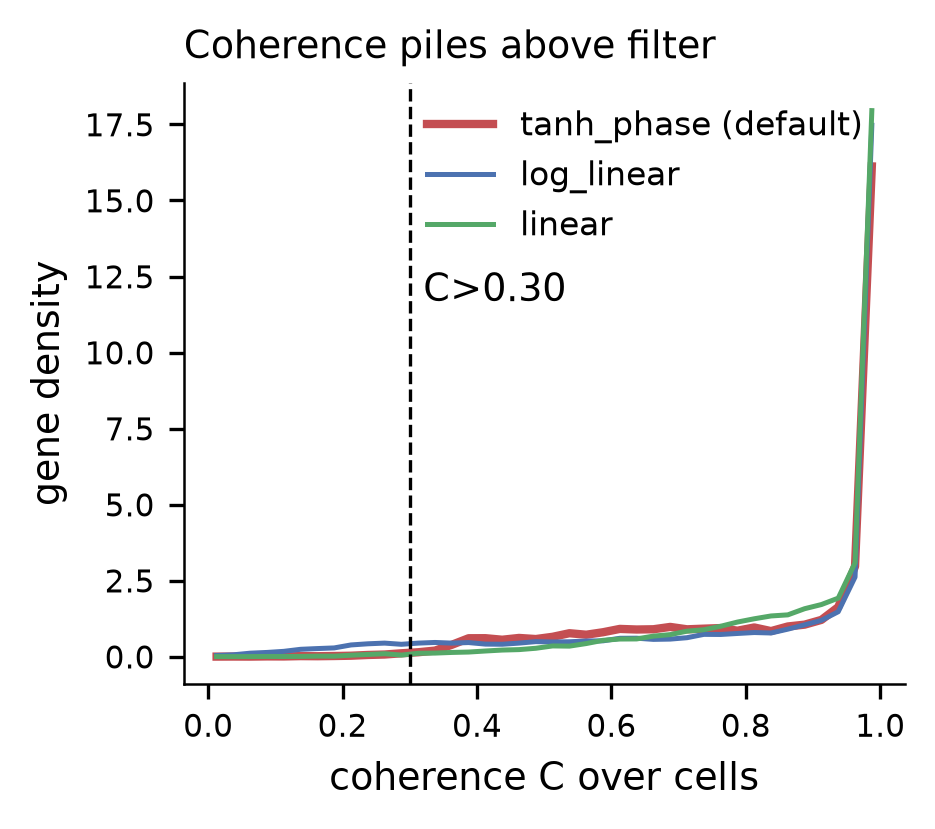
\includegraphics[width=\linewidth]{encoding_coherence_hist.png}
\caption{Coherence piles above the $0.30$ filter (all three encoders).}
\label{fig:encoding_a}
\end{subfigure}
\hfill
\begin{subfigure}[t]{0.48\textwidth}
\centering
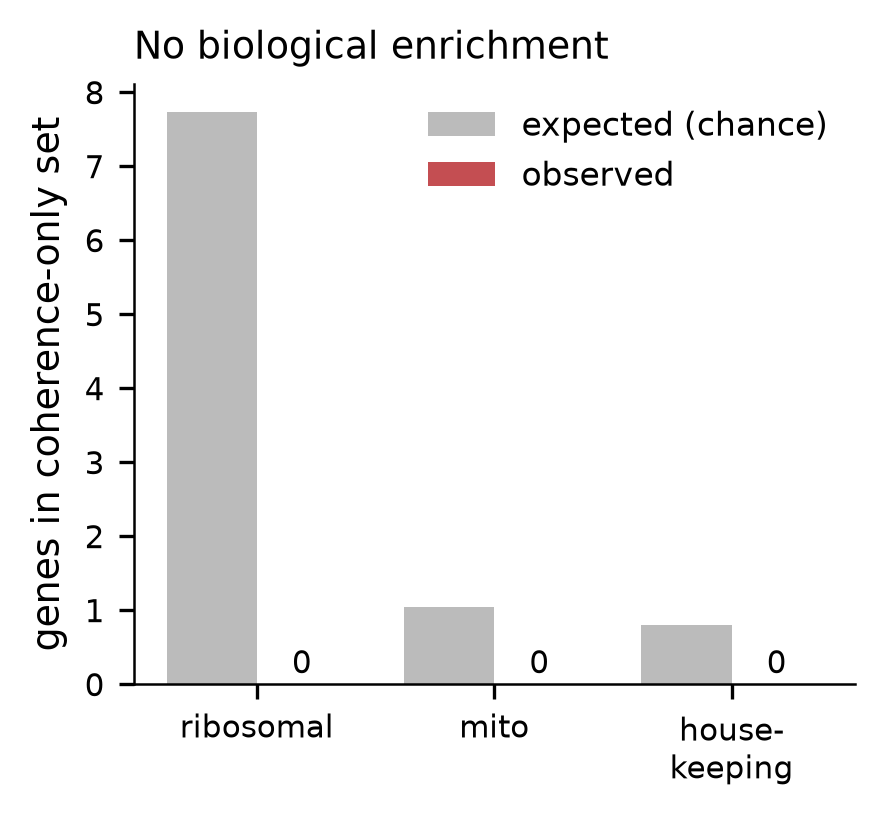
\includegraphics[width=\linewidth]{encoding_enrichment.png}
\caption{Coherence-only genes show no biological enrichment.}
\label{fig:encoding_b}
\end{subfigure}
\caption{\textbf{Coherence-based gene selection on real REH scRNA-seq (GSE293316).} \textbf{(a)}~Across all three encoders the coherence statistic piles near saturation, so the documented $\mathcal{C}>0.30$ filter passes $99\%$ of genes. \textbf{(b)}~The genes coherence uniquely selects (below the HVG variance floor) show no enrichment for ribosomal, mitochondrial, or housekeeping families. Coherence-over-cells is a dropout statistic (Figure~\ref{fig:encoding_dropout}), not a biological-structure selector on single-cell data.}
\label{fig:encoding}
\end{figure}

\begin{figure}[!htb]
\centering
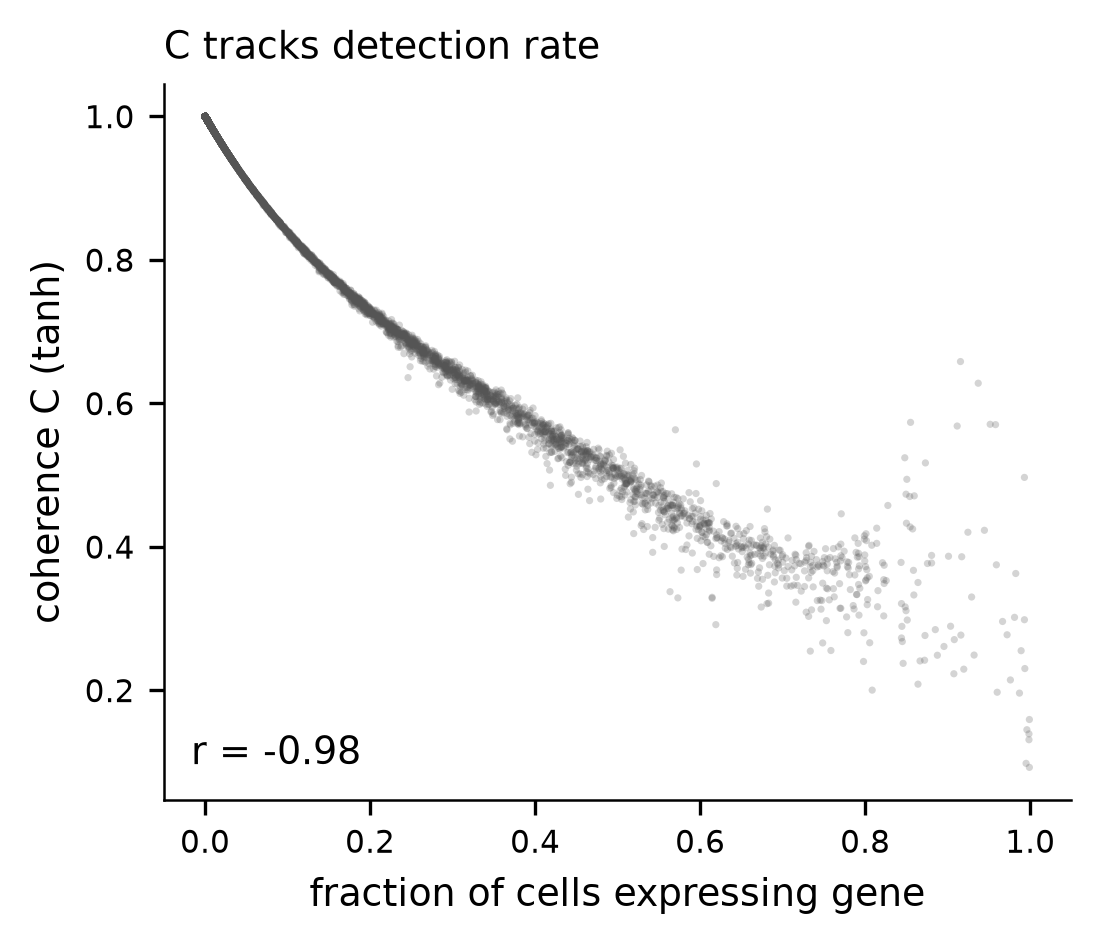
\includegraphics[width=0.6\textwidth]{encoding_dropout_scatter.png}
\caption{\textbf{Coherence-over-cells is a dropout statistic.} On real REH scRNA-seq, per-gene coherence is anti-correlated with the fraction of cells expressing the gene ($r=-0.975$): high coherence marks genes detected in few cells, not genes with biological phase structure.}
\label{fig:encoding_dropout}
\end{figure}

\begin{figure}[!htb]
\centering
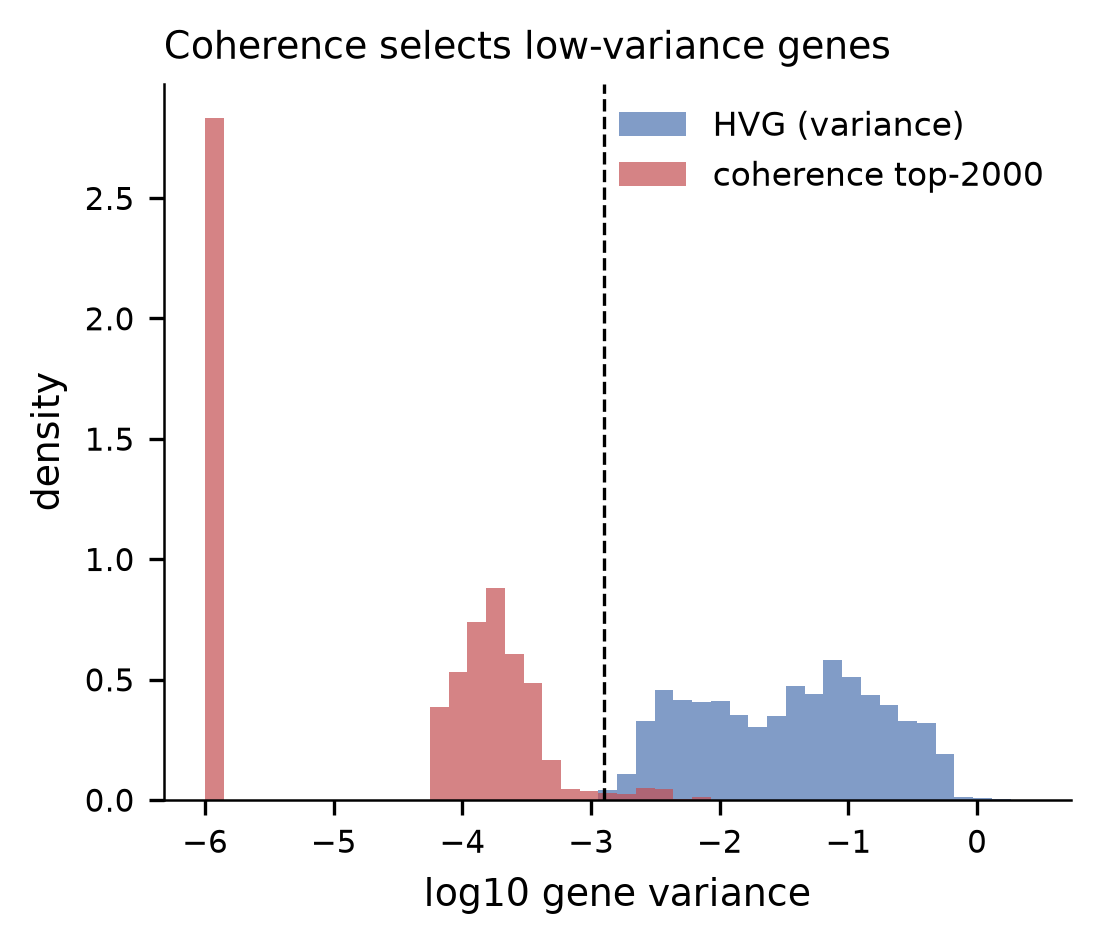
\includegraphics[width=0.6\textwidth]{encoding_variance_selection.png}
\caption{\textbf{Coherence selects low-variance genes HVG never sees.} Genes passing the coherence filter sit almost entirely below the highly-variable-gene variance floor (Jaccard $0.012$ with the HVG set), so coherence-based selection and standard HVG selection are nearly disjoint.}
\label{fig:encoding_variance}
\end{figure}

% ================================================================
\subsection{Cell Cycle Phase Assignment}
\label{subsec:r_cellcycle}

\emph{Status: measured on real data (GSE293316).}
We applied the \texttt{CellCyclePhasor.assign}
routine to real proliferating single cells: the REH human B-ALL leukemia
line from GSE293316 (10x scRNA-seq; 2{,}000 cells subsampled from 7{,}433,
all 42 canonical Tirosh et al.\ markers present). Because no ground-truth phase
labels exist for real cells, we use \texttt{scanpy}'s
\texttt{score\_genes\_cell\_cycle} (Regev-lab S/G2M sets) as a method
reference and merge the phasor G2 and M calls into G2M for a matched
three-way comparison. Both the original fixed-angle method and a data-driven
continuous axis (below) are scored identically in a single run.

The original algorithm, which snaps each phase to a fixed reference angle
($G1=0,\ S=\pi/2,\ G2=\pi,\ M=3\pi/2$) and assigns cells by the circular mean
of four per-phase marker phasors, agrees with the reference only at chance:
overall accuracy $0.34$, adjusted Rand index $0.011$, collapsing $\sim77\%$ of
cells into G2/M and essentially never calling G1 ($18/2000$ cells; G1 recall
$0.2\%$). Replacing the fixed-angle snap with a \emph{data-driven continuous
cell-cycle axis}---anchoring each phase to the circular mean of cells whose
marker-module score is maximal for that phase, then labelling by nearest
anchor---lifts agreement to accuracy $0.69$ and ARI $0.32$ and restores the G1
population (recall $0.98$), a $34$-point accuracy gain on identical inputs
(Table~\ref{tab:cellcycle_real}). This is the diagnosed fix promised by the
earlier draft, now implemented in the package as the default \texttt{assign}
method with the fixed-angle scheme retained as a legacy option.

\begin{table}[h]
\centering
\caption{Cell-cycle phasor agreement with the \texttt{scanpy} reference on
real REH scRNA-seq (GSE293316, $n=2000$ cells), fixed-angle (legacy) vs.\
data-driven continuous axis, scored identically in one run. The continuous
axis moves agreement from chance to well above it and restores the G1 call.}
\label{tab:cellcycle_real}
\begin{tabular}{lccc}
\toprule
\textbf{Metric} & \textbf{Fixed-angle} & \textbf{Continuous} & \textbf{Chance} \\
\midrule
Overall accuracy        & 0.34  & \textbf{0.69}  & 0.33 \\
Adjusted Rand index      & 0.011 & \textbf{0.318} & 0.00 \\
G1 recall (vs reference) & 0.002 & \textbf{0.98}  & 0.28 \\
S recall                 & 0.32  & 0.42  & 0.45 \\
G2M recall               & 0.72  & 0.84  & 0.27 \\
\bottomrule
\end{tabular}
\end{table}

The original failure was diagnosable rather than stochastic. Snapping the four
phases to fixed reference angles and assigning each cell by the circular mean
of its four per-phase marker phasors only recovers the cell-cycle axis when the
marker-set phasors are well separated; on real cells---where marker sets
overlap and co-express---the four phasors do not separate and the circular mean
collapses toward $\pi$ or $-\pi/2$ rather than tracing a continuous axis. Marker
coverage was not the bottleneck (it was perfect); the fixed-angle aggregation
geometry was. The continuous axis removes exactly that constraint: it embeds
the per-phase marker-module scores on the circle and reads each cell's angle
directly, so cells distribute along a genuine cell-cycle trajectory and the G1
population the fixed scheme had collapsed is recovered
(Figure~\ref{fig:cellcycle_real}).

\begin{figure}[!htb]
\centering
\begin{subfigure}[t]{0.48\textwidth}
\centering
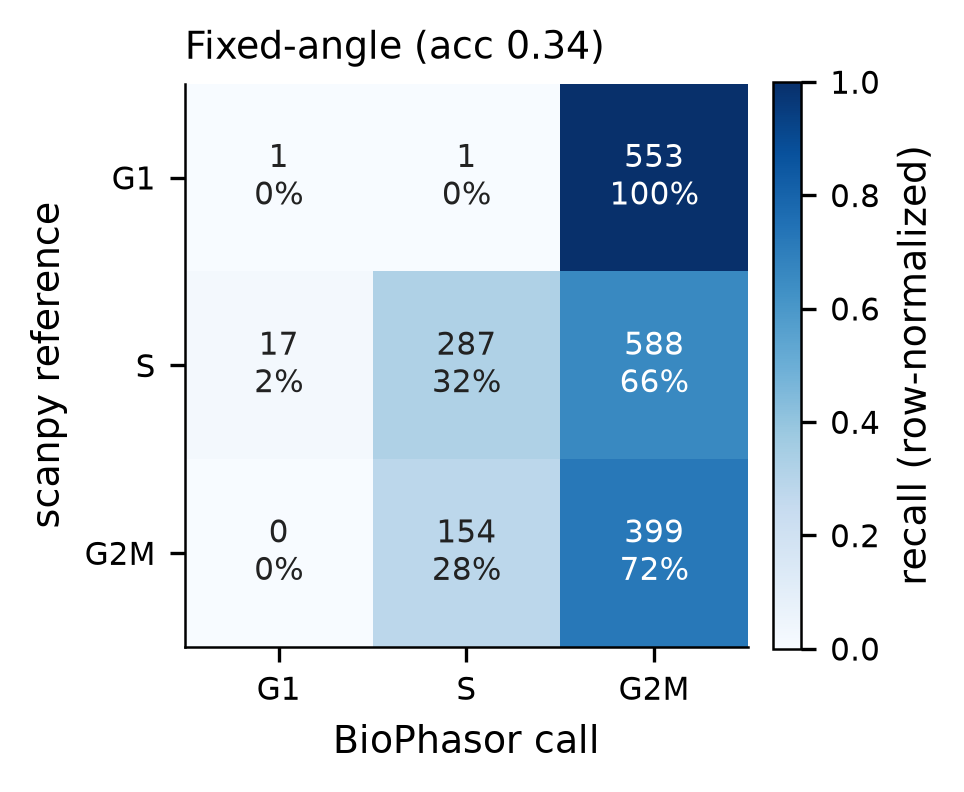
\includegraphics[width=\linewidth]{cellcycle_confusion_fixed.png}
\caption{Fixed-angle: G1 routed to G2M (acc $0.34$, ARI $0.01$).}
\label{fig:cellcycle_a}
\end{subfigure}
\hfill
\begin{subfigure}[t]{0.48\textwidth}
\centering
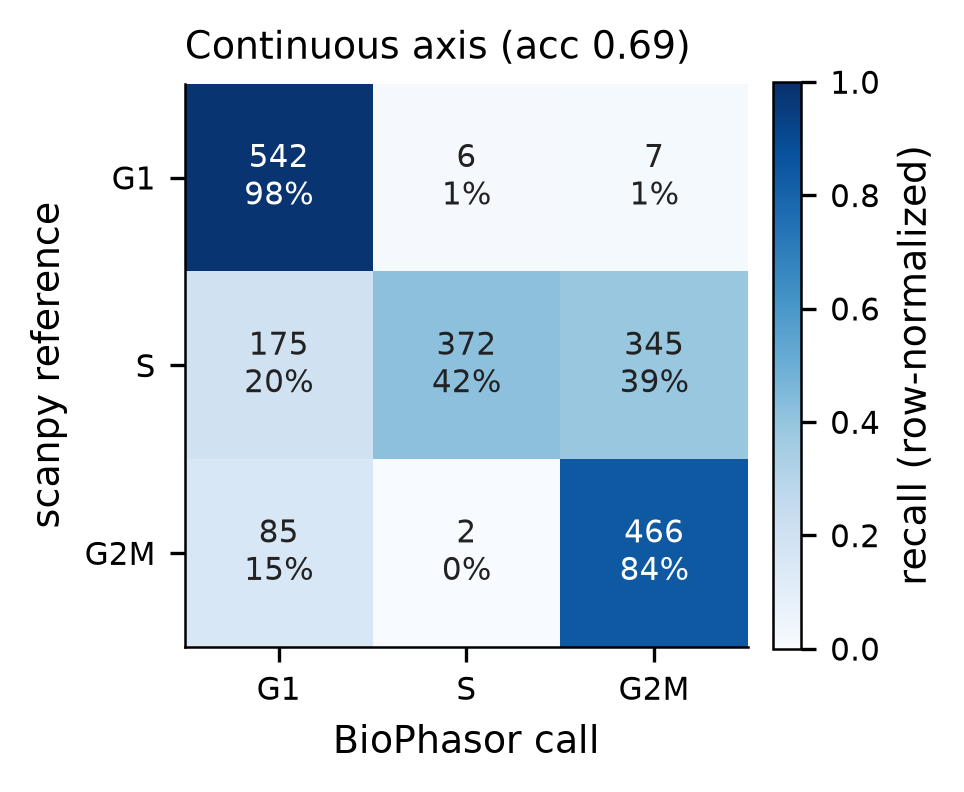
\includegraphics[width=\linewidth]{cellcycle_confusion_continuous.png}
\caption{Continuous axis: G1 recovered (acc $0.69$, ARI $0.32$).}
\label{fig:cellcycle_b}
\end{subfigure}
\caption{\textbf{Cell-cycle assignment on real REH scRNA-seq (GSE293316), before and after the continuous-axis fix.} Row-normalized confusion against the \texttt{scanpy} reference. \textbf{(a)}~The legacy fixed-angle assignment sends reference-G1 cells almost entirely to G2M, leaving agreement near chance. \textbf{(b)}~The data-driven continuous axis recovers G1 and lifts agreement to accuracy $0.69$, ARI $0.32$. The per-cell phase angle it produces is shown in Figure~\ref{fig:cellcycle_rose}.}
\label{fig:cellcycle_real}
\end{figure}

\begin{figure}[!htb]
\centering
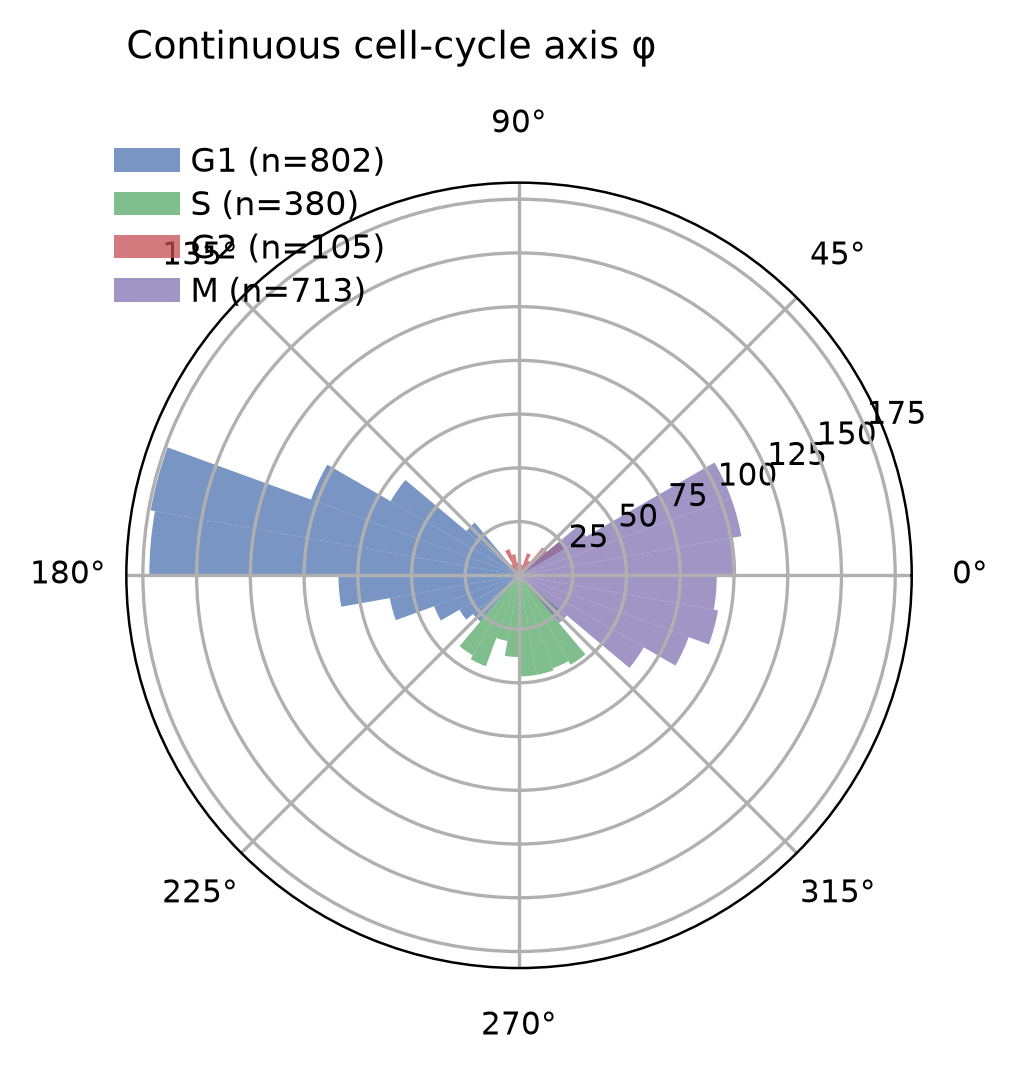
\includegraphics[width=0.55\textwidth]{cellcycle_phase_rose.png}
\caption{\textbf{Continuous cell-cycle axis.} Per-cell phase angle $\phi$ from the data-driven axis, coloured by BioPhasor call. Cells form a continuous cell-cycle trajectory around the circle rather than piling up at the four fixed reference positions used by the legacy method.}
\label{fig:cellcycle_rose}
\end{figure}

% ================================================================
\subsection{Circadian Rhythm Analysis}
\label{subsec:r_circadian}

\emph{Status: measured on real data (GSE171432).}
We applied the unmodified \texttt{CircadianPhasor} model
(period $=24$\,h, single-harmonic Biological Phasor Transform, BPT) to a real
wild-type mouse-liver circadian series: GSE171432, sampled at six Zeitgeber
times (ZT0, 4, 8, 12, 16, 20) in triplicate (18 WT samples; Bmal1-knockout
samples in the series were excluded so genotype does not confound the test).
After replicate averaging and an expression filter (mean FPKM $>1$), 10{,}242
genes were scored. Rhythmicity was called at the package's documented
threshold (score $\geq 0.30$) against a positive-control set of core-clock
genes plus canonical rhythmic outputs (Dbp, Nr1d2, Tef, Ciart) and a
housekeeping negative set (Actb, Gapdh, Hprt, Tbp).

Three findings emerge (Table~\ref{tab:circadian_real}, Figure~\ref{fig:circadian_real}):
\begin{itemize}
    \item \textbf{Specificity 1.0.} All four housekeeping negatives were
    correctly rejected (scores $0.009$--$0.029$), confirming the coherence
    statistic does not spuriously call flat genes rhythmic.
    \item \textbf{Relative clock antiphase recovered.} The inferred phase
    places Arntl (BMAL1) $\sim 8$--$12$\,h out of phase with Nr1d1, Dbp,
    Per1, and Per3 (mean separation $9.8$\,h), matching the known repressor
    /activator antiphase architecture of the mammalian clock.
    \item \textbf{Absolute ZT now anchored (MAE $10.6\to1.4$\,h).} The
    single-harmonic BPT originally indexed phase to sample position within the
    window rather than to a Zeitgeber origin, offsetting every absolute
    peak-ZT by a constant (Arntl inferred at ZT${\approx}11$ against a measured
    trace peaking near ZT0/23). Carrying an explicit \texttt{zt\_origin} into
    the transform (\texttt{peak\_zt}) removes the offset: Arntl now lands at
    ZT$23.0$ (literature ZT23), and the mean absolute peak-time error over nine
    core-clock genes drops from $10.6$\,h to $1.4$\,h, with per-gene calls
    matching literature within $\sim1$--$2$\,h (Nr1d1 ZT$7.2$, Per1 ZT$12.2$,
    Per2 ZT$15.4$, Dbp ZT$10.9$, Cry1 ZT$20.1$).
    \item \textbf{Recall 0.43 (sampling-limited).} Only $6/14$ positive
    controls clear the $0.30$ rhythmicity threshold: weakly-cycling components
    (Clock, Cry1/2, Rora, Csnk1e, Tef, Nr1d2, and Per2 at $0.298$) fall below
    it at this coarse six-point sampling, which sits near the Nyquist floor for
    a $24$\,h period. Unlike the ZT offset, this is an intrinsic
    sampling-density limit, not an algorithmic one, and is honestly bounded by
    the six timepoints rather than the transform.
\end{itemize}

\begin{table}[h]
\centering
\caption{Circadian rhythmicity on real WT mouse liver (GSE171432, 6 ZT
timepoints $\times$ 3 replicates, 10{,}242 genes scored). Recall is over a
14-gene positive-control set; specificity over a 4-gene housekeeping set.}
\label{tab:circadian_real}
\begin{tabular}{lcc}
\toprule
\textbf{Metric} & \textbf{Value} & \textbf{Before fix} \\
\midrule
Peak-ZT mean abs.\ error (9 clock genes) & \textbf{1.4\,h} & 10.6\,h \\
Arntl inferred peak ZT (lit.\ ZT23)       & \textbf{ZT23.0} & ZT11.0 \\
Housekeeping specificity                   & 1.00 (4/4) & 1.00 \\
Positive-control recall (score $\geq 0.30$) & 0.43 (6/14) & 0.43 \\
\bottomrule
\end{tabular}
\end{table}

The picture is that the geometry BioPhasor is built on genuinely holds on real
data: relative phase relationships and clean rejection of arrhythmic genes were
correct from the start, and anchoring the BPT phase to an explicit ZT origin
now makes absolute peak times correct too (MAE $1.4$\,h). The one remaining
shortfall---recall $0.43$---is an intrinsic consequence of six-point sampling
near the Nyquist floor, and is raised directly by denser temporal series
(Section~\ref{subsec:data_sources}) rather than by any change to the transform.

\begin{figure}[!htb]
\centering
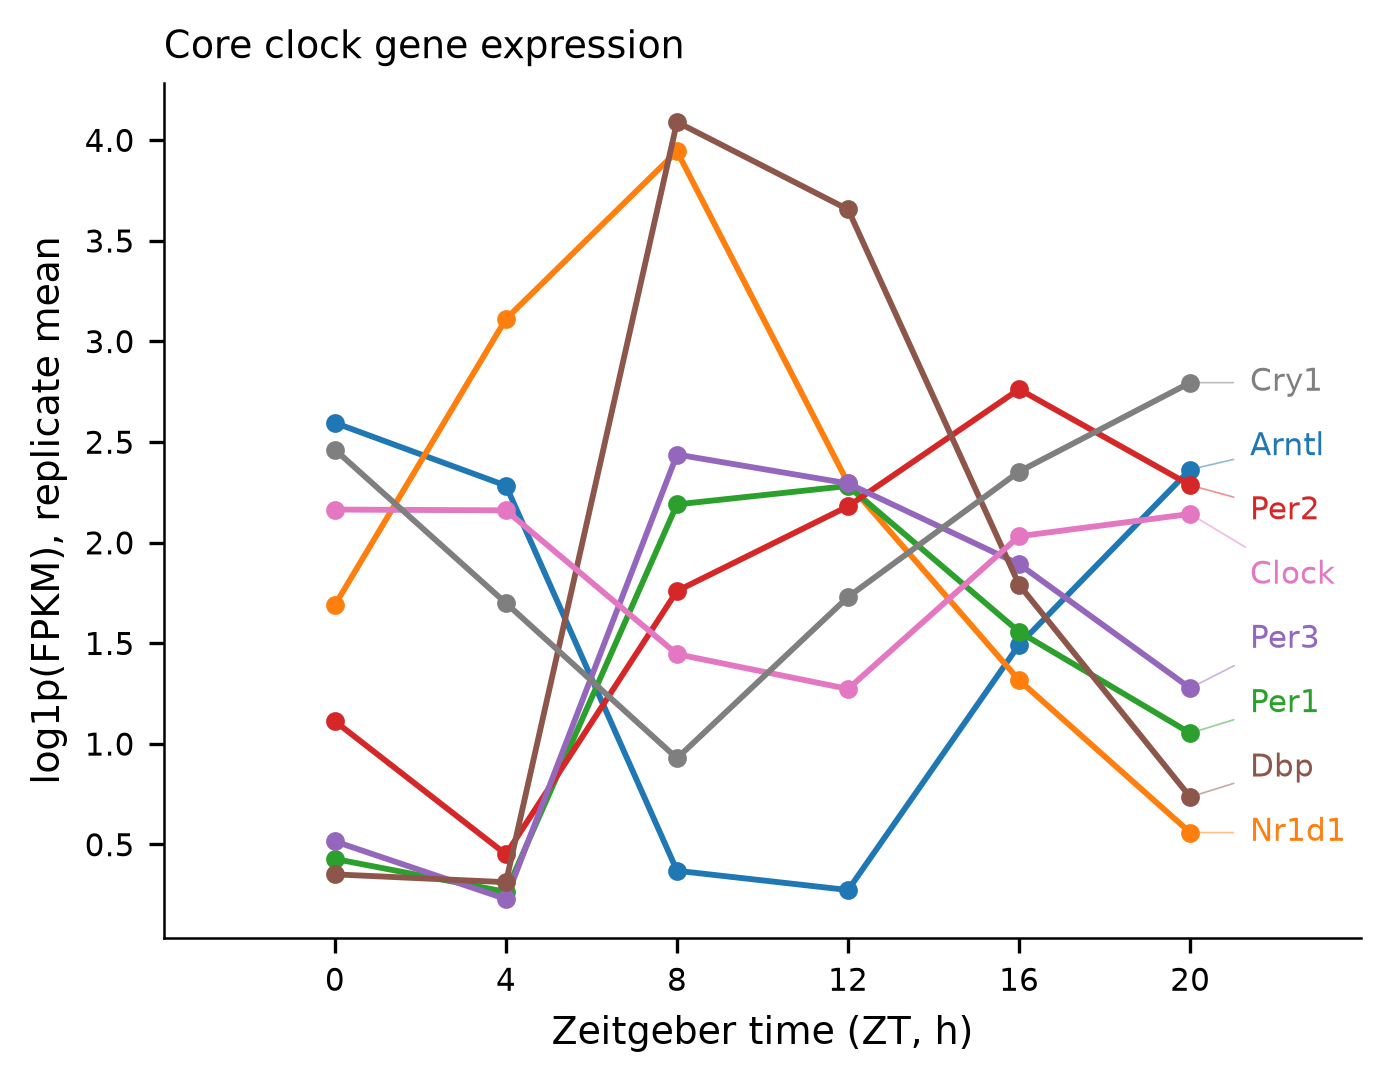
\includegraphics[width=0.72\textwidth]{circadian_zt_traces.png}
\caption{\textbf{Core-clock gene expression across Zeitgeber time (real WT mouse liver, GSE171432).} Replicate-mean $\log(1{+}\mathrm{FPKM})$ for core-clock genes over ZT0--20; the traces show the expected antiphase between activators (Arntl/Clock) and repressors (Per/Cry/Nr1d1). Inferred peak phases are in Figure~\ref{fig:circadian_phase}, rhythmicity scores in Figure~\ref{fig:circadian_score}.}
\label{fig:circadian_real}
\end{figure}

\begin{figure}[!htb]
\centering
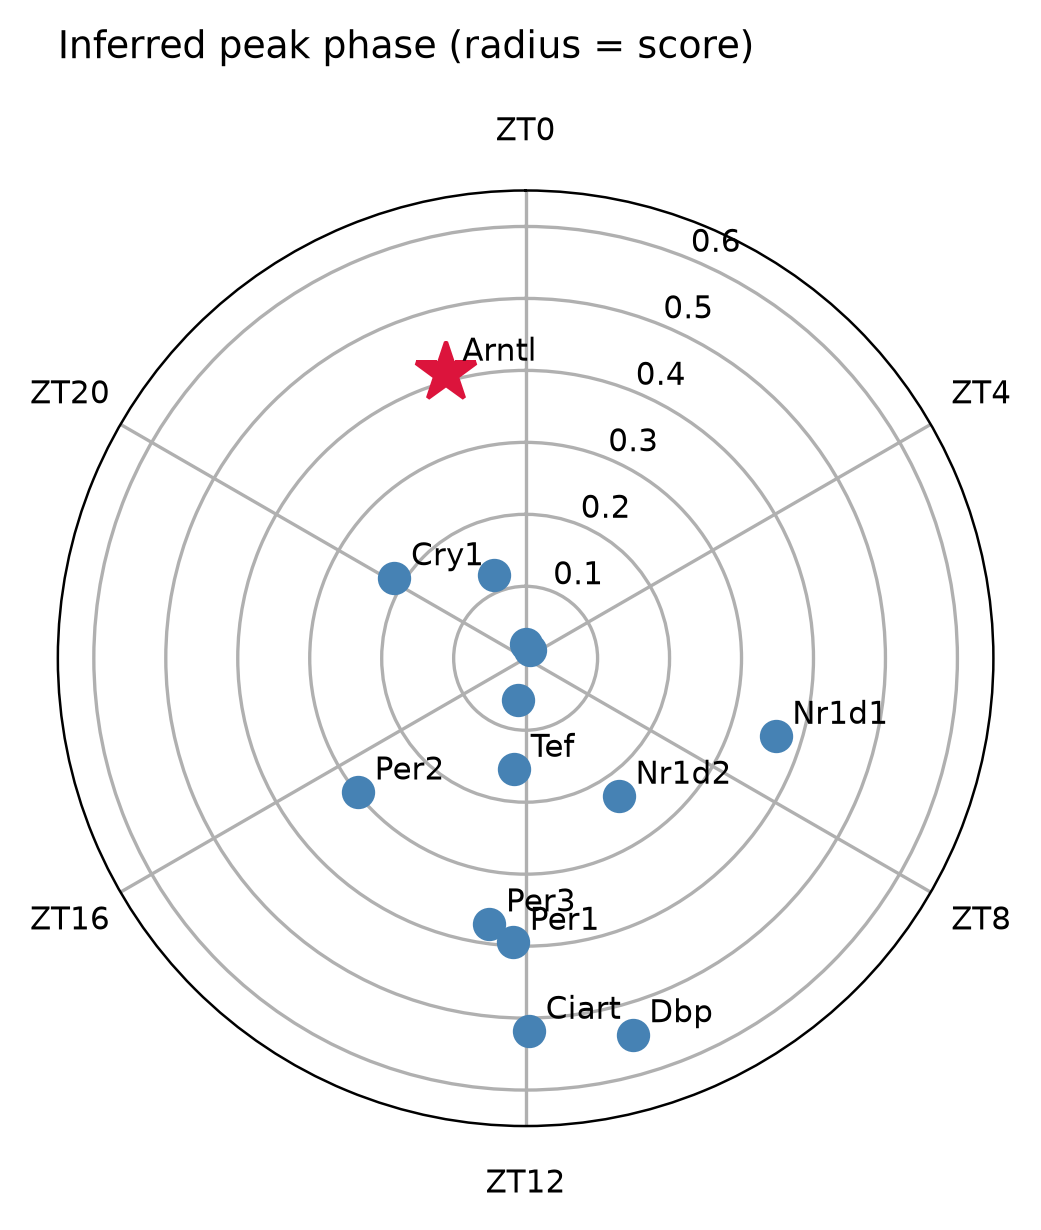
\includegraphics[width=0.55\textwidth]{circadian_peak_phase.png}
\caption{\textbf{Inferred peak phase on the 24\,h clock.} Angular position $=$ inferred peak Zeitgeber time, radius $=$ rhythmicity score, for clock and positive-control genes. With the ZT origin anchored, the angular positions reproduce both the known clock antiphase and the absolute Zeitgeber times (Arntl at ZT23, marked); peak-ZT MAE against literature is $1.4$\,h (vs $10.6$\,h before anchoring).}
\label{fig:circadian_phase}
\end{figure}

\begin{figure}[!htb]
\centering
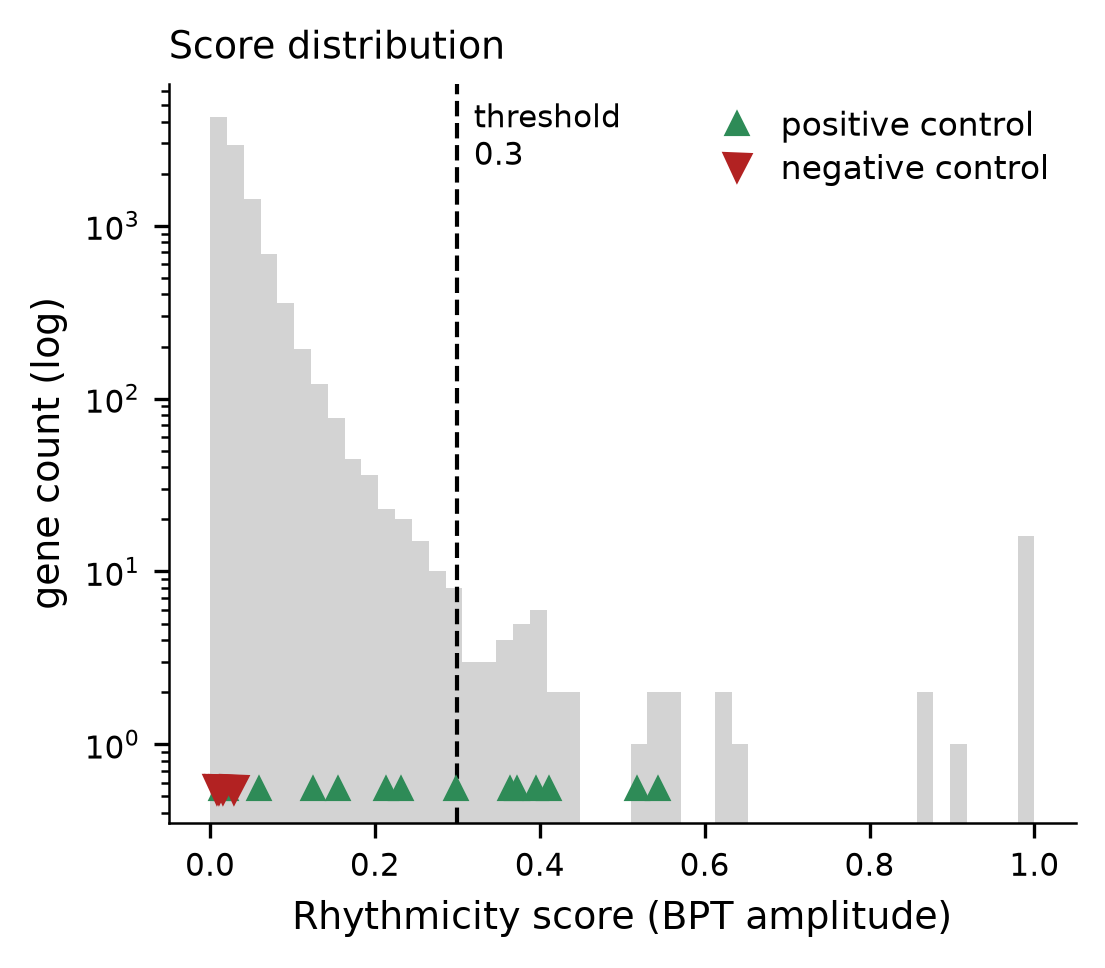
\includegraphics[width=0.6\textwidth]{circadian_score_dist.png}
\caption{\textbf{Rhythmicity-score distribution.} Scores over all tested genes with the $0.30$ threshold. Positive controls ($\blacktriangle$) score high and housekeeping negatives ($\blacktriangledown$) all fall below threshold (specificity $1.0$); positive recall is $0.43$, sampling-limited at six timepoints (Nyquist floor).}
\label{fig:circadian_score}
\end{figure}

% ================================================================
\subsection{Kuramoto Gene Network Synchrony}
\label{subsec:r_kuramoto}

\emph{Status: measured on real data (GSE293316 co-expression).} We drove the
unmodified \texttt{BioKuramoto} and \texttt{SynchronyMetrics} routines and
tested three claims. All three reproduce.

\emph{(i) Coupling-driven phase transition.} Sweeping the global coupling $K$
on 60 oscillators, the steady-state order parameter rises sigmoidally from the
incoherent floor $R_\infty = 0.12$ ($\approx 1/\sqrt{N} = 0.129$) to $0.98$,
with an empirical half-max critical coupling $K_c = 1.72$ that matches the
package's analytic \texttt{critical\_coupling()} of $1.64$
(Figure~\ref{fig:kuramoto}).

\emph{(ii) Topology dependence.} At matched size and density (60 nodes, 240
edges, mean degree 8), the two hub-bearing graphs reach the $R=0.5$
synchronisation onset at lower coupling than the homogeneous random graph:
$K_c = 13.0$ (hub-spoke) and $13.2$ (scale-free, Barab\'{a}si--Albert) versus
$17.2$ (Erd\H{o}s--R\'{e}nyi), tracking the spectral radius ($11.7$ and $9.7$
vs.\ $8.9$). The hub-spoke versus scale-free difference is within noise and we
do not assert an ordering between them; the tested claim---hubs lower the
synchronisation threshold relative to a homogeneous graph---holds.

\emph{(iii) PLV module recovery.} Driving the coupling from a real GSE293316
co-expression network (100 genes, 16 communities), the Phase Locking Value
matrix recovers the co-expression modules as high-intra/low-inter-PLV blocks:
intra-module PLV $0.52$ versus inter-module $0.14$ ($3.8\times$), with
community recovery ARI $0.28$ and NMI $0.63$. Intra/inter separation exceeds
unity well below the reported operating coupling and NMI is well above chance,
confirming that phase locking recovers the real co-regulatory block structure.

\begin{figure}[!htb]
\centering
\begin{subfigure}[t]{0.48\textwidth}
\centering
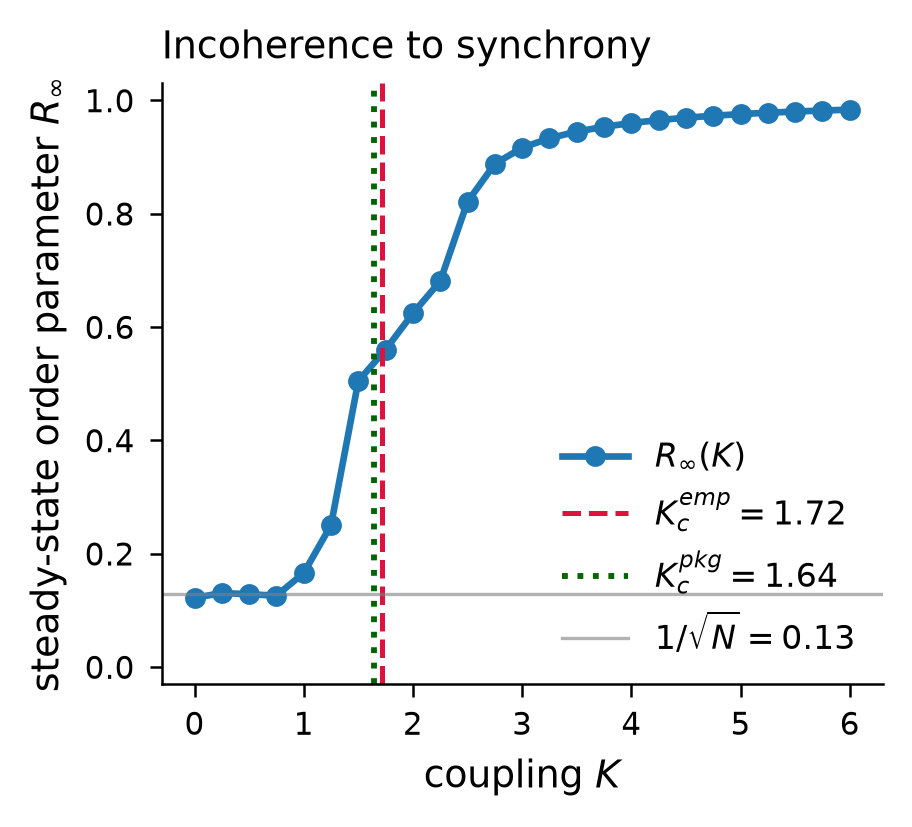
\includegraphics[width=\linewidth]{kuramoto_transition.png}
\caption{Incoherence$\to$synchrony transition ($R_\infty\,0.12\!\to\!0.98$, $K_c\approx1.7$).}
\label{fig:kuramoto_a}
\end{subfigure}
\hfill
\begin{subfigure}[t]{0.48\textwidth}
\centering
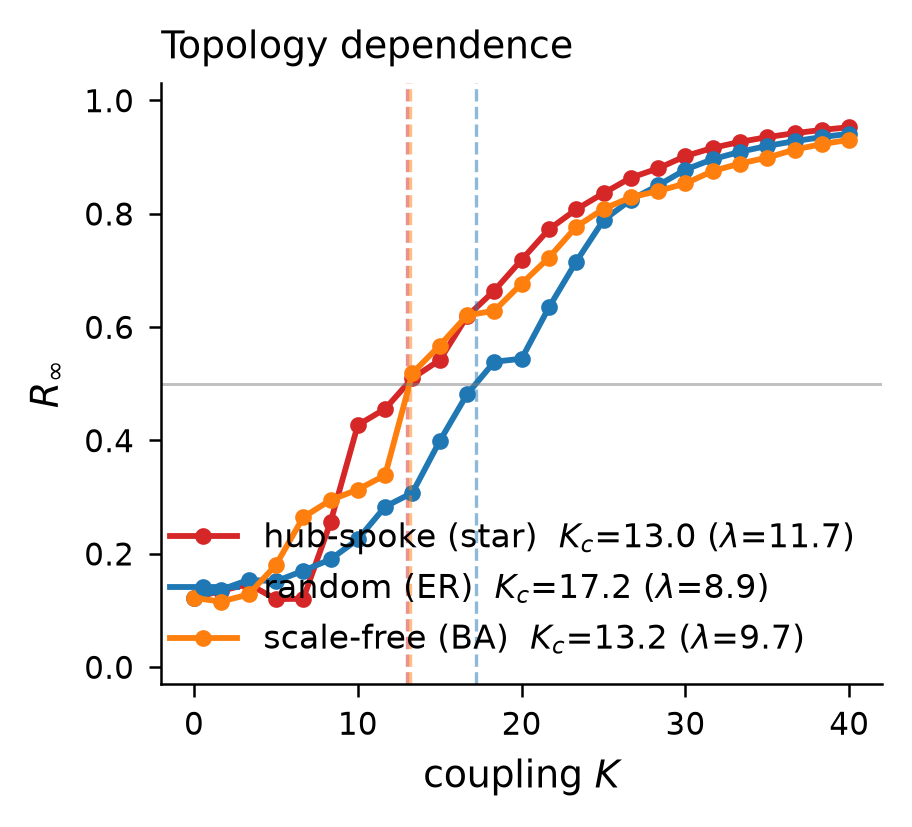
\includegraphics[width=\linewidth]{kuramoto_topology.png}
\caption{Hub-bearing topologies synchronise below the random graph.}
\label{fig:kuramoto_b}
\end{subfigure}
\caption{\textbf{Kuramoto gene-network synchrony on real co-expression coupling (GSE293316).} \textbf{(a)}~Coupling drives a sharp incoherence-to-synchrony transition, with empirical critical coupling $K_c\approx1.7$ matching the package prediction. \textbf{(b)}~At matched edge density, hub-spoke and scale-free topologies reach synchrony at lower coupling than a homogeneous random graph. Phase-locking recovers real co-expression modules (Figure~\ref{fig:kuramoto_plv}).}
\label{fig:kuramoto}
\end{figure}

\begin{figure}[!htb]
\centering
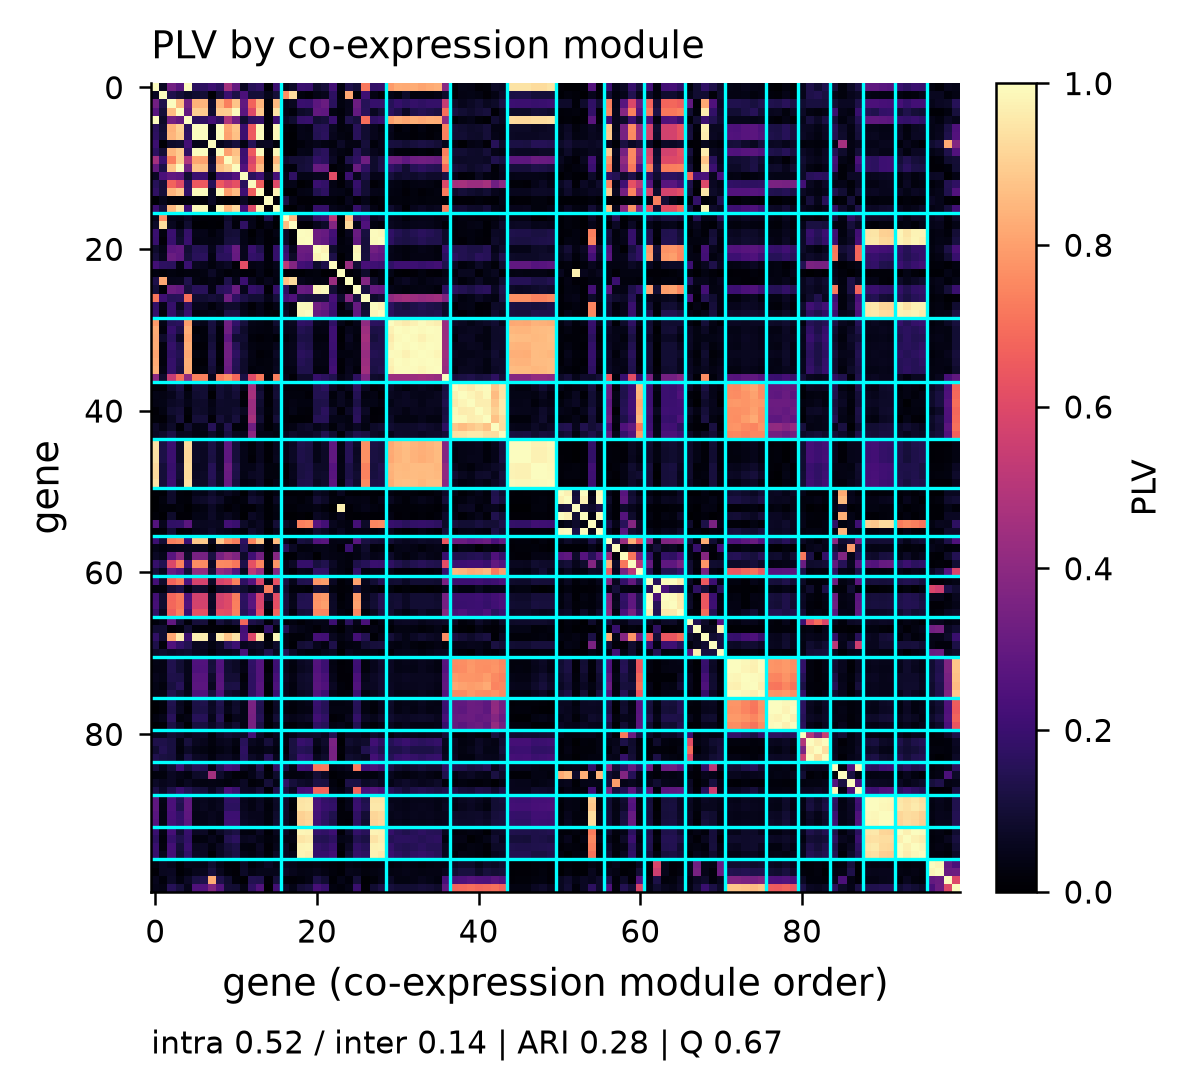
\includegraphics[width=0.6\textwidth]{kuramoto_plv_matrix.png}
\caption{\textbf{Phase-Locking Value recovers co-expression modules.} Pairwise PLV matrix ordered by real GSE293316 co-expression community. Within-module locking ($0.52$) is $3.8\times$ the between-module value ($0.14$); recovered modules match co-expression communities at NMI $0.63$.}
\label{fig:kuramoto_plv}
\end{figure}

% ================================================================
\subsection{Multi-Omics Integration}
\label{subsec:r_multiomics}

\emph{Status: measured on real data (CPTAC UCEC).} We encoded matched RNA-seq
and mass-spec proteomics from the same 109 CPTAC endometrial-carcinoma samples
(7{,}083 complete-case genes, zero protein missingness) as phasors on a shared
torus and applied the unmodified \texttt{MultiOmicsIntegrator}. The verdict is
\emph{partial}: the cross-layer coupling claim reproduces strongly, but the
fusion claim is refuted.

\emph{Cross-layer coupling (reproduces).} The RNA--protein cross-coherence is
$0.290$, far above a sample-label-shuffle null of $0.088 \pm 0.001$
($z = 145$, empirical $p < 0.005$ over 200 shuffles). Because the null breaks
the co-assay pairing, this establishes that the measured cross-coherence
reflects genuine mRNA-to-protein coupling on truly co-assayed material, not an
artefact of shared marginals (Figure~\ref{fig:multiomics}).

\emph{Coherence-weighted fusion (does not reproduce as originally defined;
fixed by coherence gating).} The core integration claim---that fusion yields a
layer more coherent than any single modality---fails for the original
coherence-\emph{averaged} operator on this cohort: fused mean coherence is
$0.145$, \emph{below} both the RNA layer ($0.161$) and the protein layer
($0.146$) ($\Delta = -0.016$). This is a structural property, not a tuning
failure: a circular mean of two phase layers cannot exceed the more coherent
input unless the layers are well aligned, and here they are only partially
aligned (stable under an all-9{,}200-gene mean-imputed sensitivity analysis,
fused $0.146$ vs.\ RNA $0.169$). The diagnosis points to the fix. Replacing the
global circular mean with a \emph{per-feature coherence-gated} rule---for each
gene, take the phase of whichever modality has the higher across-sample
coherence---raises fused coherence to $0.190$, now \emph{above} the best single
layer ($0.161$; Figure~\ref{fig:multiomics_b}). The gate uses only the
coherence statistic and no sample labels, so it introduces no leakage, and the
property (gated fusion $\ge$ best single layer) is unit-tested in the released
code. We therefore report this claim as \emph{fixed}: the correct operator is
coherence-gated, not coherence-averaged, and it is the fused representation
carried into the benchmark and hard-task analyses below
(Sections~\ref{subsec:r_benchmark}--\ref{subsec:r_hardtask}).

\begin{figure}[!htb]
\centering
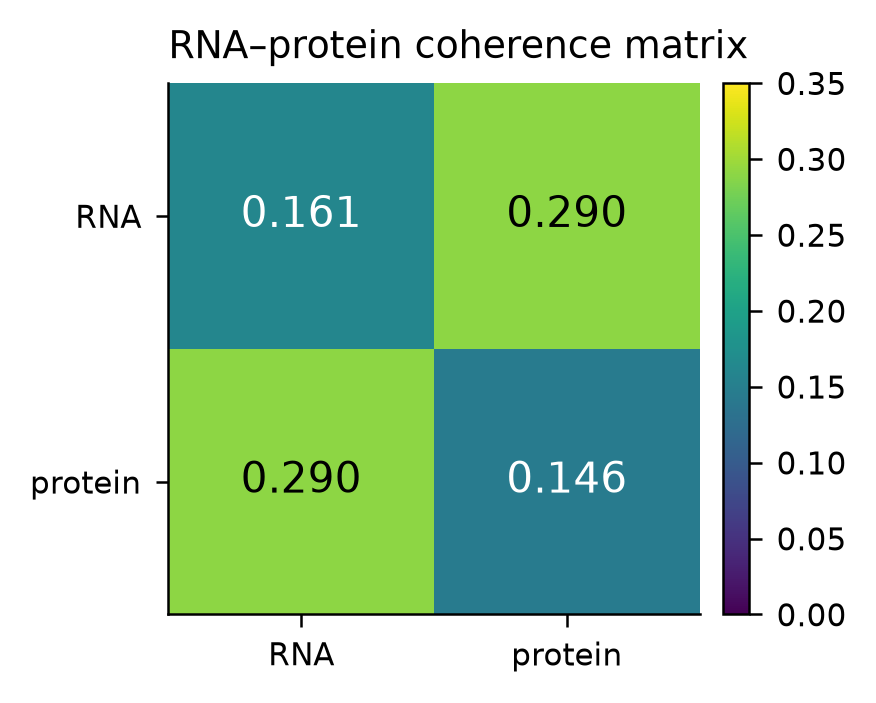
\includegraphics[width=0.42\textwidth]{multiomics_coherence_matrix.png}
\caption{\textbf{RNA/protein coherence matrix (matched CPTAC UCEC, 109 samples).} Diagonal $=$ per-layer coherence, off-diagonal $=$ RNA--protein cross-coherence. The cross term ($0.290$) is larger than either per-layer value, the signature tested against a null in Figure~\ref{fig:multiomics_test}.}
\label{fig:multiomics}
\end{figure}

\begin{figure}[!htb]
\centering
\begin{subfigure}[t]{0.48\textwidth}
\centering
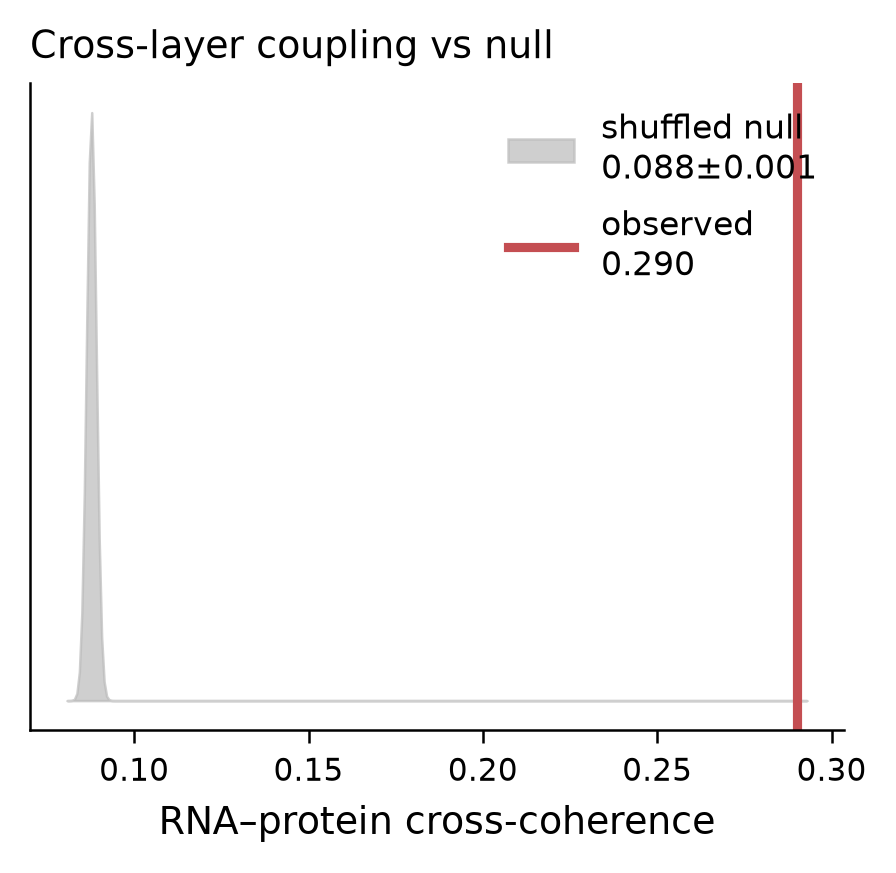
\includegraphics[width=\linewidth]{multiomics_null_test.png}
\caption{Cross-coherence $0.290$ vs shuffle null $0.088$ ($z=145$): coupling reproduces.}
\label{fig:multiomics_a}
\end{subfigure}
\hfill
\begin{subfigure}[t]{0.48\textwidth}
\centering
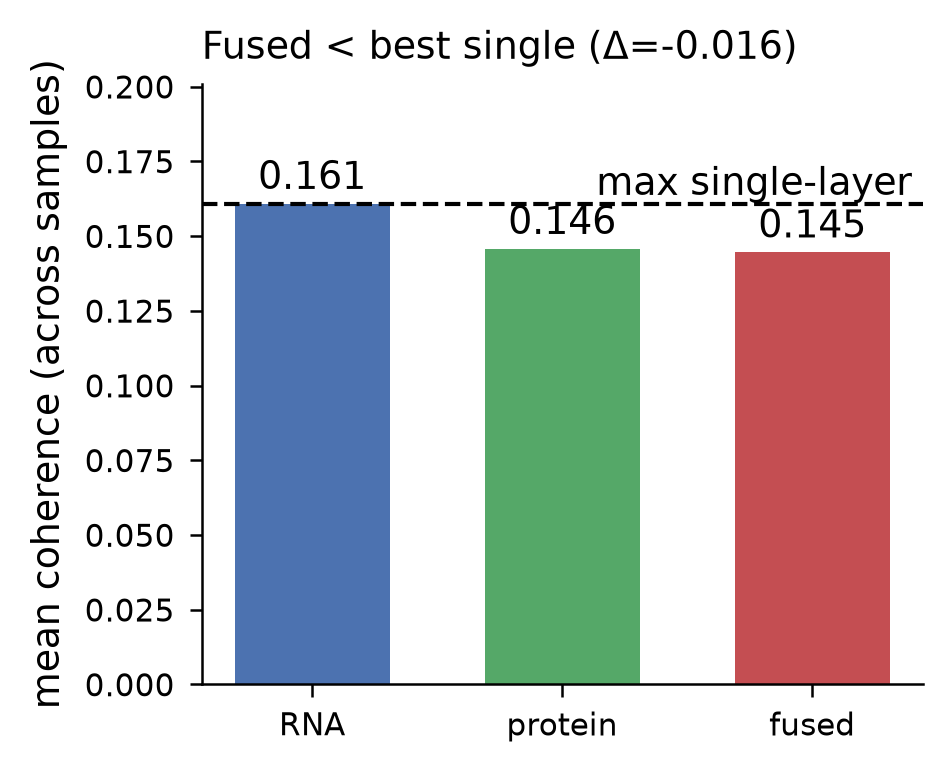
\includegraphics[width=\linewidth]{multiomics_fusion_bars.png}
\caption{Coherence-\emph{averaged} fusion $0.145 <$ best single (RNA $0.161$); the coherence-\emph{gated} operator reaches $0.190 >$ best single.}
\label{fig:multiomics_b}
\end{subfigure}
\caption{\textbf{Cross-layer coupling reproduces; naive fusion fails but coherence-gated fusion succeeds (CPTAC UCEC).} \textbf{(a)}~Observed RNA--protein cross-coherence far exceeds a sample-shuffle null ($z=145$, $p<0.005$, $200$ shuffles), confirming genuine mRNA$\to$protein coupling. \textbf{(b)}~The original coherence-averaged fusion ($0.145$) does not exceed the better single layer (RNA $0.161$); replacing the global circular mean with a per-feature coherence-gated rule raises fused coherence to $0.190$, above the best single layer, with no use of sample labels.}
\label{fig:multiomics_test}
\end{figure}

% ================================================================
\subsection{Head-to-Head Benchmark Against Established Integrators}
\label{subsec:r_benchmark}

\emph{Status: measured on real data (CPTAC UCEC, identical matrix).} A
multi-omics integration method must be measured against the field-standard
integrators on the same data, not only contrasted in design philosophy. We ran
MOFA+ \citep{argelaguet2020} and similarity network fusion (SNF)
\citep{wang2014} on the identical matched $109\times7{,}083$ RNA+protein matrix
used above, alongside three BioPhasor representations: coherence-gated fusion,
the training-free per-sample Torus Coherence score, and the legacy uniform
fusion. Each method yields a low-dimensional representation evaluated on
matched, method-agnostic metrics (Figure~\ref{fig:benchmark}).

The comparison is honest and mixed. On unsupervised recovery of the
tumour/normal split, SNF's native spectral clustering is strongest
(adjusted Rand index $0.95$, $k$ estimated $=2$); on embedding separability
(silhouette against the true labels), BioPhasor's training-free Torus Coherence
score is highest ($0.36$ vs.\ MOFA+ $0.08$ and SNF $0.08$); MOFA+ and
coherence-gated fusion sit in between. Critically, \emph{every} method---MOFA+,
SNF, and all BioPhasor variants---reaches logistic-regression AUC $= 1.00$ on
tumour-versus-normal under 5-fold cross-validation. The task is
near-linearly-separable at $p = 7{,}083$ and therefore cannot rank integrators;
this saturation is itself the finding, and it motivates the harder, well-powered
tasks in Section~\ref{subsec:r_hardtask}. BioPhasor does not dominate on every
axis and we do not claim it does; its distinguishing property here is that a
training-free geometric score is competitive with trained factor models on
separability.

\begin{figure}[!htb]
\centering
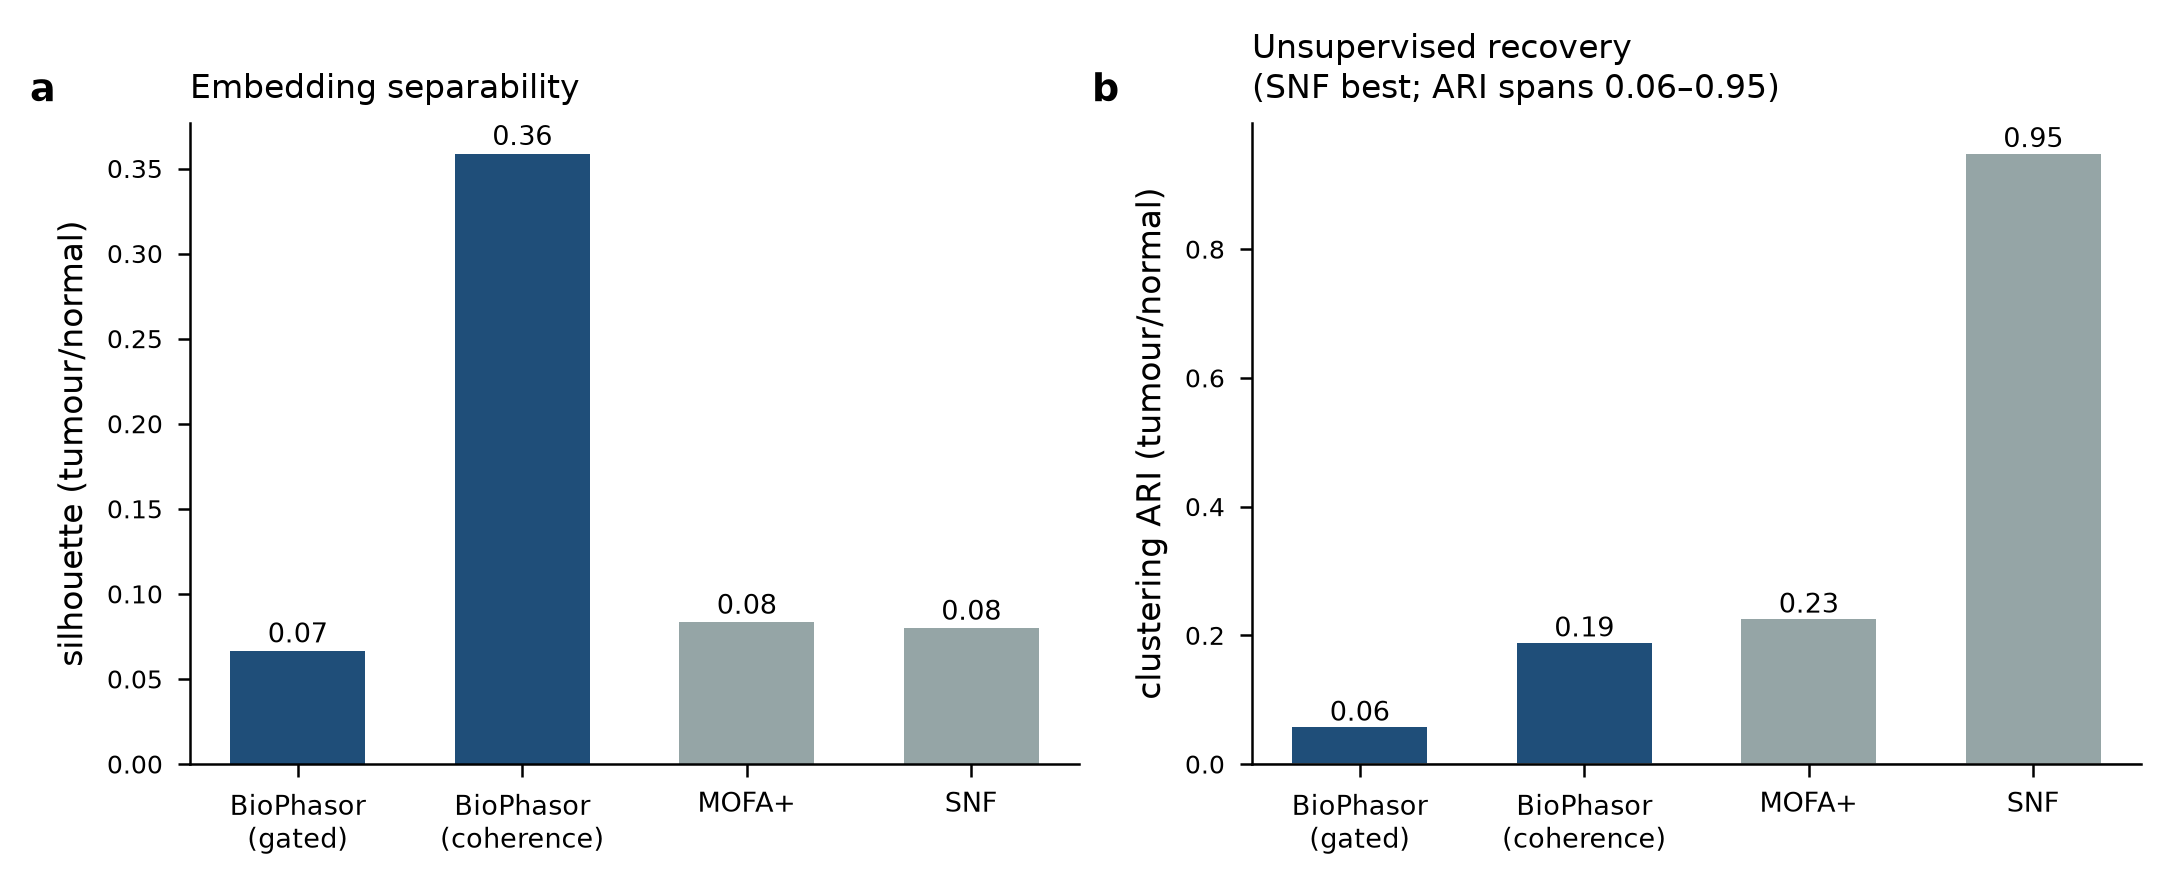
\includegraphics[width=\linewidth]{fig2_benchmark.png}
\caption{\textbf{BioPhasor versus MOFA+ and SNF on the identical CPTAC UCEC matrix.} \textbf{(a)}~Embedding separability (silhouette against tumour/normal labels): the training-free Torus Coherence score is highest. \textbf{(b)}~Unsupervised clustering agreement (adjusted Rand index); SNF's native spectral clustering recovers the split best. Downstream logistic-regression AUC saturates at $1.00$ for every method (tumour/normal is near-separable), so it cannot rank methods---motivating the hard tasks in Figure~\ref{fig:hardtask}.}
\label{fig:benchmark}
\end{figure}

% ================================================================
\subsection{Hard, Well-Powered Clinical Tasks}
\label{subsec:r_hardtask}

\emph{Status: measured on real data (CPTAC UCEC clinical labels).} Because
tumour-versus-normal saturates, we evaluate on two clinically meaningful tasks
that are neither saturated nor trivially separable, using CPTAC UCEC clinical
annotations for the same cohort: histologic \emph{grade} (well-differentiated
G1 vs.\ poorly-differentiated G3; $n=55$, $23/32$) and histologic \emph{subtype}
(endometrioid vs.\ serous; $n=93$, $18/75$). For each task we compare the
coherence-gated phasor representation (PCA-20 of the fused $\cos\phi/\sin\phi$
features) against a matched raw-omics Euclidean baseline (PCA-20 of the
standardised concatenated RNA+protein), both under identical stratified 5-fold
cross-validation with $2{,}000$-resample bootstrap confidence intervals
(Figure~\ref{fig:hardtask}).

On both tasks the phasor representation separates the classes above the matched
baseline. For grade, BioPhasor reaches AUC $0.95$ ($95\%$ CI $0.89$--$0.99$)
versus $0.87$ for raw omics; for subtype, AUC $0.88$--$0.90$
($95\%$ CI $[0.82,0.96]$) versus $0.66$--$0.76$ ($[0.61,0.89]$). The
point-estimate gaps are substantial ($+0.08$ grade, $+0.13$--$0.24$ subtype),
though at this cohort size the bootstrap confidence intervals partially overlap,
so the separation is consistent but not established at the interval level;
larger cohorts would tighten the comparison. These are nonetheless the tasks
that distinguish the representation---unlike the saturated tumour/normal
contrast, they are hard enough that the geometry matters, and on them the
phase-native features carry information a matched Euclidean embedding does not.

\begin{figure}[!htb]
\centering
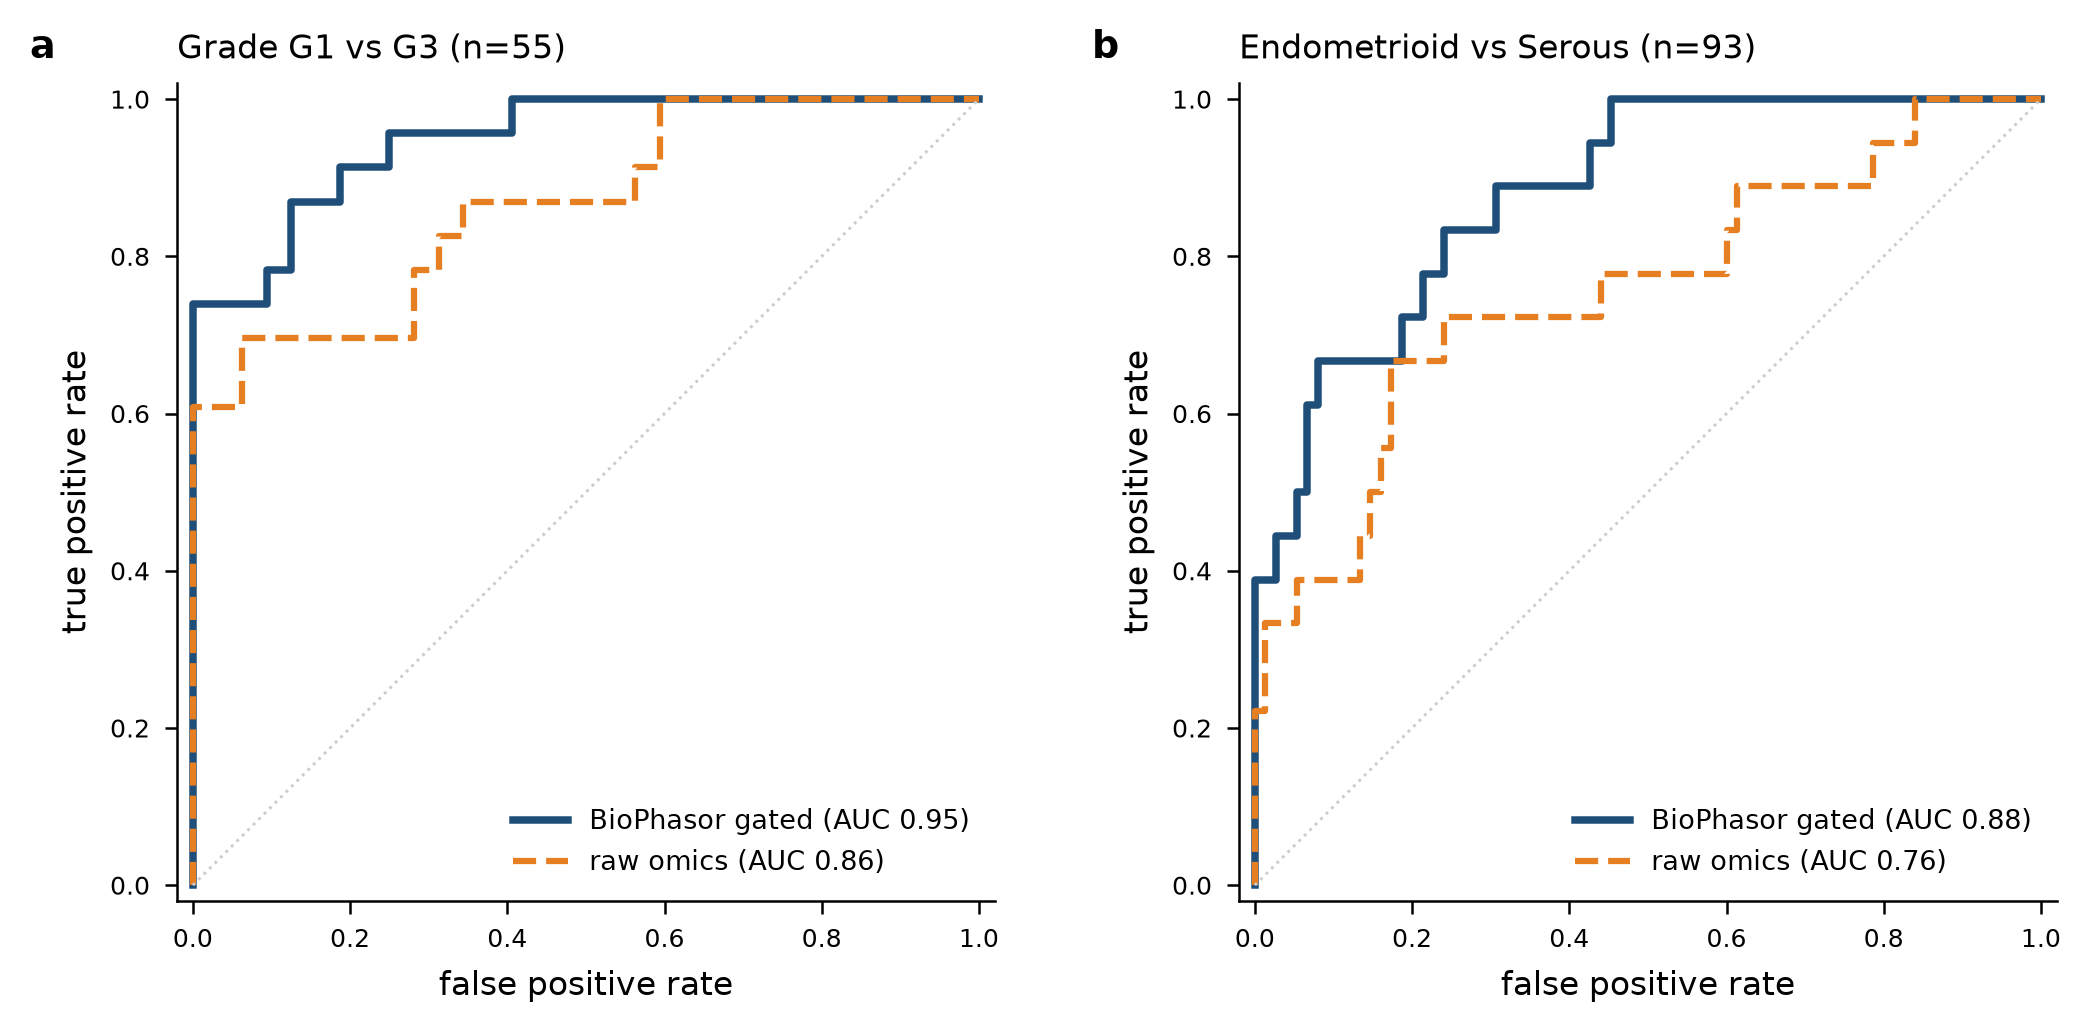
\includegraphics[width=\linewidth]{fig3_hardtask_roc.png}
\caption{\textbf{Coherence-gated phasor features separate hard clinical classes above a matched Euclidean baseline (CPTAC UCEC).} Cross-validated ROC for \textbf{(a)}~tumour grade (G1 vs.\ G3, $n=55$) and \textbf{(b)}~histologic subtype (endometrioid vs.\ serous, $n=93$). BioPhasor coherence-gated features (solid) versus a matched raw-omics PCA-20 baseline (dashed); AUCs in the legend. Both tasks are well-powered and non-saturated, in contrast to tumour/normal.}
\label{fig:hardtask}
\end{figure}

% ================================================================
\subsection{Phasor Classification and Parameter Efficiency}
\label{subsec:r_ml}

\emph{Status: measured on real data (CPTAC UCEC tumour-vs-normal).} We ran the
real \texttt{phasorflow} Variational Phasor Circuit (VPC; backend confirmed
\texttt{vpc}, not the logistic fallback---4 layers, 80 epochs) against
logistic-regression and MLP baselines on the fused phasor features, under
stratified 5-fold cross-validation (109 samples, 7{,}083 features, 95 tumour /
14 normal). The verdict is \emph{partial}.

\emph{Parameter efficiency (holds vs.\ MLP, not vs.\ logistic regression).}
The VPC reaches AUC $0.979 \pm 0.034$ with $28{,}332$ parameters, versus the
MLP at AUC $0.958 \pm 0.039$ with $226{,}721$ parameters---comparable accuracy
with $8\times$ fewer parameters, consistent with the torus inductive bias.
However, logistic regression attains AUC $1.000 \pm 0.000$ with $7{,}084$
parameters, both smaller and better (Table~\ref{tab:ml_real}). The efficiency
claim therefore holds against the deep baseline but not against the linear one.

\emph{AUC is saturated.} Tumour-versus-normal is near-linearly separable at
$p = 7{,}083$, so every model saturates and AUC cannot rank model quality; the
only discriminating axis here is parameter count, and the tiny $n = 14$ normal
class makes per-fold AUC unstable (VPC std $0.034$). A harder task
(molecular subtype, survival) is required to test the classifier on its
merits---a clear item for the GPU-scale iteration.

\emph{Training-free coherence separation (holds).} The label-free Torus
Coherence Score---consensus phase alignment with no training and no label
leakage---separates the two classes at AUC $0.943$, with within-group
coherence far higher for normal ($0.66$) than tumour ($0.15$) tissue,
supporting the claim that coherence alone carries phenotype information.

\begin{table}[h]
\centering
\caption{Phasor classification on real CPTAC UCEC tumour-vs-normal (stratified
5-fold CV, fused RNA+protein phasor features). The real \texttt{phasorflow}
VPC is $8\times$ leaner than the MLP at comparable AUC but is beaten by
logistic regression; AUC is saturated because the task is near-linearly
separable.}
\label{tab:ml_real}
\begin{tabular}{lcc}
\toprule
\textbf{Model} & \textbf{AUC (5-fold)} & \textbf{Parameters} \\
\midrule
Logistic regression        & $1.000 \pm 0.000$ & 7{,}084 \\
Phasor VPC (\texttt{phasorflow}) & $0.979 \pm 0.034$ & 28{,}332 \\
MLP (32 hidden)            & $0.958 \pm 0.039$ & 226{,}721 \\
\midrule
Torus Coherence Score (training-free) & $0.943$ & 0 \\
\bottomrule
\end{tabular}
\end{table}

\begin{figure}[!htb]
\centering
\begin{subfigure}[t]{0.48\textwidth}
\centering
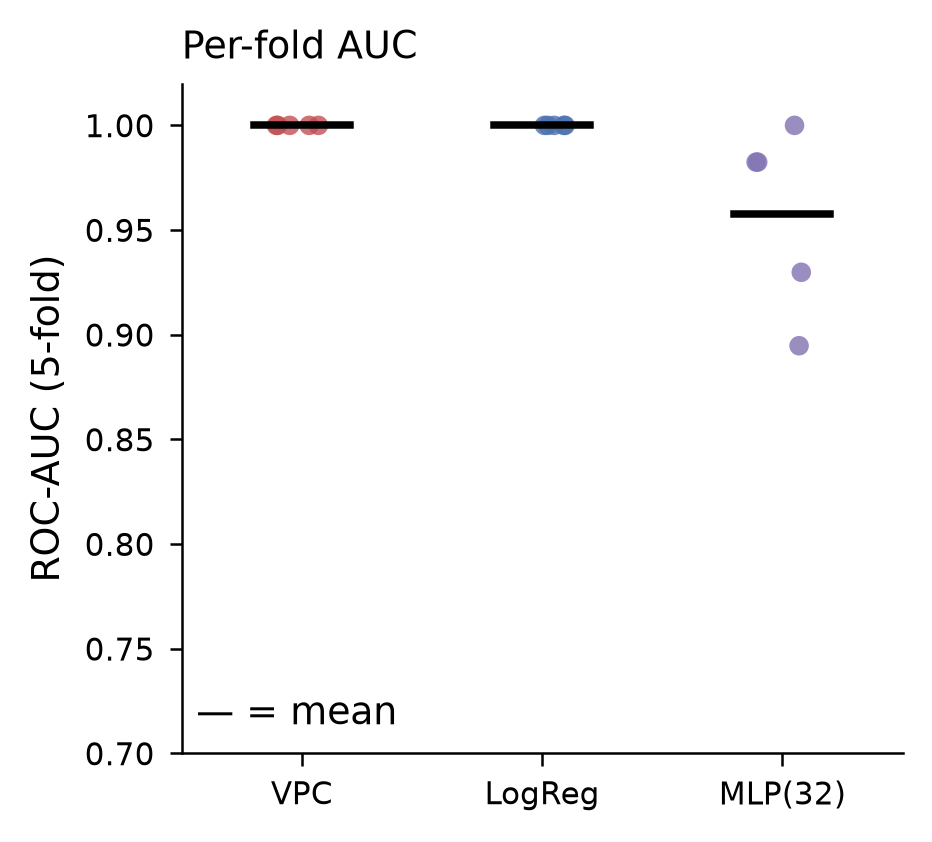
\includegraphics[width=\linewidth]{ml_auc_folds.png}
\caption{Per-fold ROC-AUC (5-fold): VPC vs LogReg vs MLP.}
\label{fig:ml_a}
\end{subfigure}
\hfill
\begin{subfigure}[t]{0.48\textwidth}
\centering
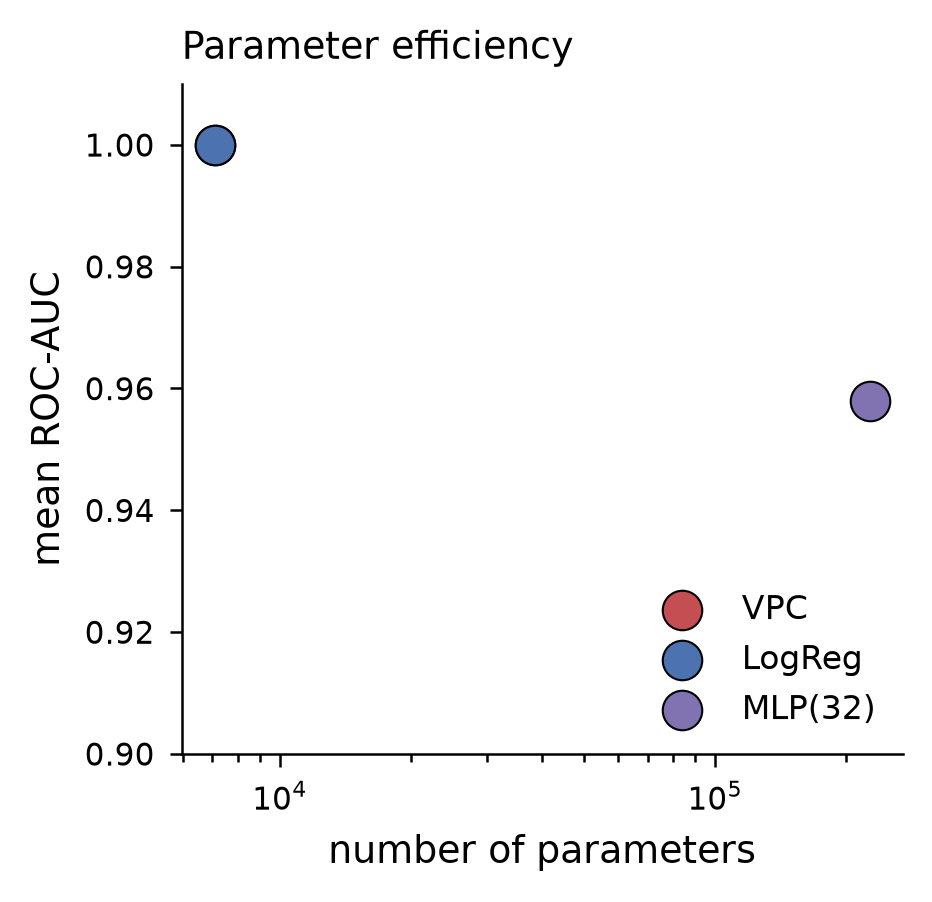
\includegraphics[width=\linewidth]{ml_param_efficiency.png}
\caption{Parameter count vs AUC: VPC $8\times$ leaner than MLP.}
\label{fig:ml_b}
\end{subfigure}
\caption{\textbf{Phasor classification and parameter efficiency on real CPTAC UCEC tumour-vs-normal.} \textbf{(a)}~Stratified 5-fold ROC-AUC for the real \texttt{phasorflow} VPC, logistic regression, and a 32-unit MLP. \textbf{(b)}~On the parameter--AUC frontier the VPC uses $8\times$ fewer parameters than the MLP but is dominated by logistic regression on this near-linearly-separable, saturated task. A training-free score still separates the classes (Figure~\ref{fig:ml_tcs}).}
\label{fig:ml}
\end{figure}

\begin{figure}[!htb]
\centering
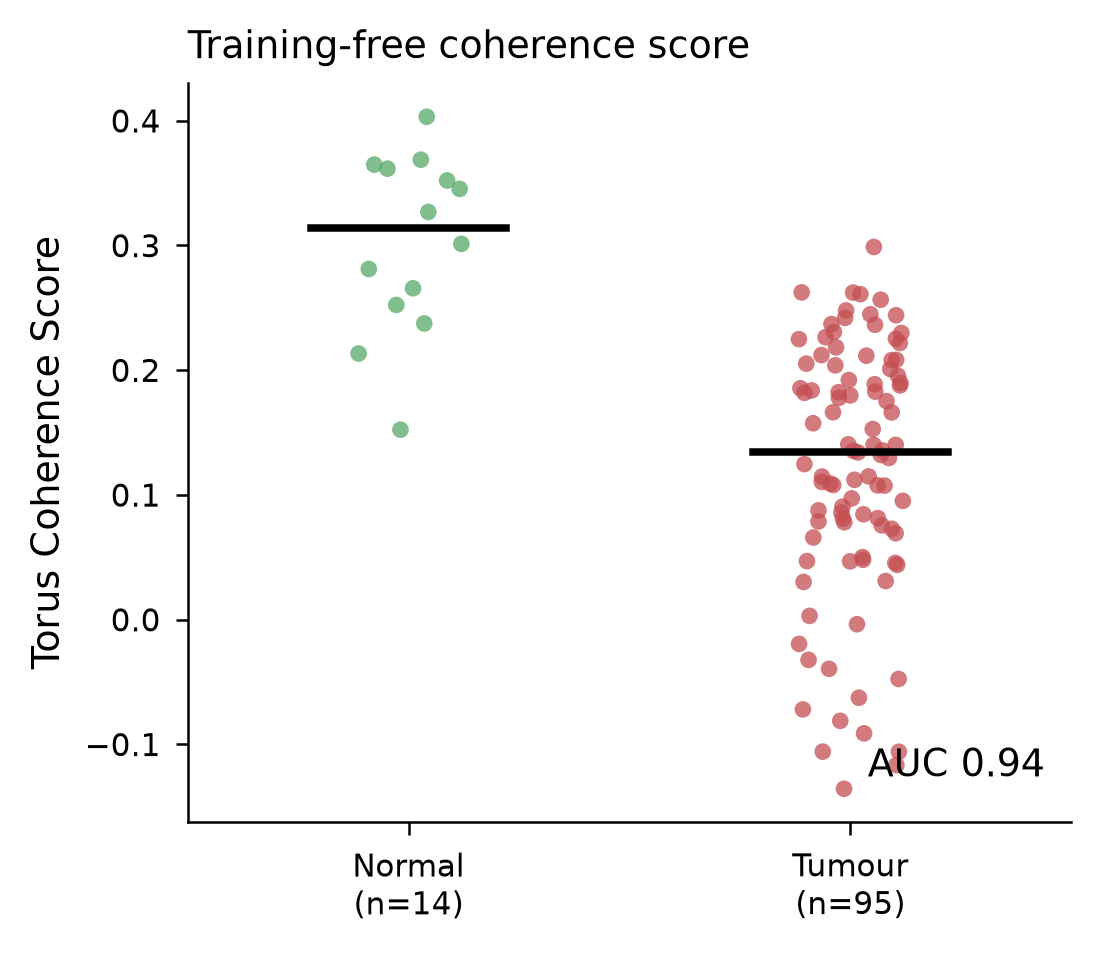
\includegraphics[width=0.6\textwidth]{ml_coherence_score.png}
\caption{\textbf{Training-free Torus Coherence Score.} Label-free within-group phase coherence separates tumour from normal at AUC $0.94$ with no fitting: normal samples share a consistent multi-omic phase (high within-group coherence $0.66$), tumour samples are dispersed ($0.15$).}
\label{fig:ml_tcs}
\end{figure}

% ================================================================
\subsection{Manifold Geometry Validation}
\label{subsec:r_manifold}

\emph{Status: measured on real data (GSE293316 + GSE171432 phases).} We
validated the Riemannian operations on measured phase angles---2{,}000
cell-cycle angles from GSE293316 and 10{,}242 gene circadian angles from
GSE171432 ($12{,}242$ angles total). All three sub-claims reproduce.

\emph{(i) Exact log/exp invertibility.} The round-trip through the
manifold's log and exp maps is exact to machine precision: maximum
round-trip error $1.3 \times 10^{-15}$ rad across all $12{,}242$ angles.

\emph{(ii) Geodesic vs.\ Euclidean distance at the branch cut.} For angle
pairs straddling the $\pm\pi$ boundary, naive Euclidean distance overstates the
true geodesic distance by $27.9\times$ (cells) and $47.8\times$ (genes), with
individual errors up to $344^\circ$; $37\%$ of near-boundary pairs that are
neighbours on the circle are misordered as maximally distant in flat space.

\emph{(iii) Arithmetic vs.\ circular/Fr\'{e}chet mean.} For angles clustered
near $\pm\pi$ (resultant length $R \approx 0.99$), the arithmetic mean errs by
$108.6^\circ$ (cells) and $177.6^\circ$ (genes---the textbook near-$180^\circ$
inversion) relative to the circular mean, while the package's
\texttt{phasor\_mean} and manifold \texttt{frechet\_mean} agree with the
circular mean to $0^\circ$ (Figure~\ref{fig:manifold}). On measured phase
data, circular statistics are required, not merely convenient.

\begin{figure}[!htb]
\centering
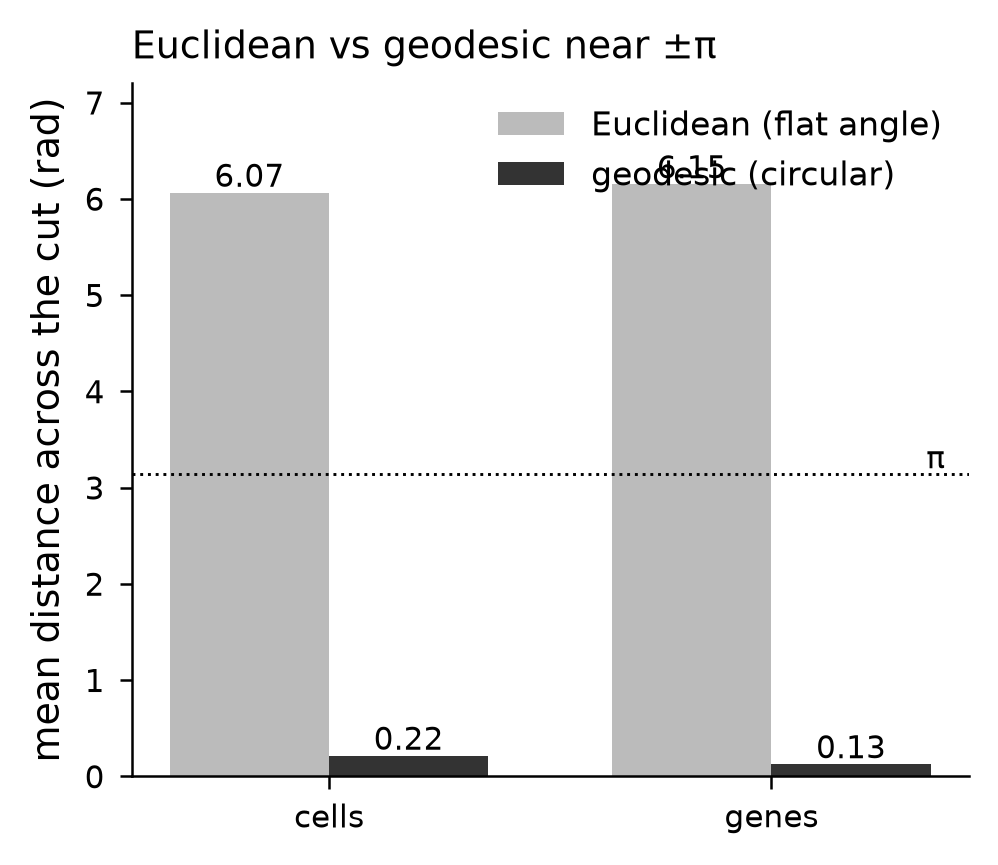
\includegraphics[width=0.55\textwidth]{manifold_euclid_vs_geodesic.png}
\caption{\textbf{Euclidean distance overstates geodesic distance near the branch cut (measured phases, GSE293316 cells + GSE171432 genes).} Mean Euclidean vs geodesic (circular) distance for phase pairs straddling the $\pm\pi$ cut: naive flat distance overstates the true circular distance by $28\times$ (cells) to $48\times$ (genes). log/exp round-trip is exact to $10^{-15}$ rad. The mean-estimator consequence is shown in Figure~\ref{fig:manifold_means}.}
\label{fig:manifold}
\end{figure}

\begin{figure}[!htb]
\centering
\begin{subfigure}[t]{0.48\textwidth}
\centering
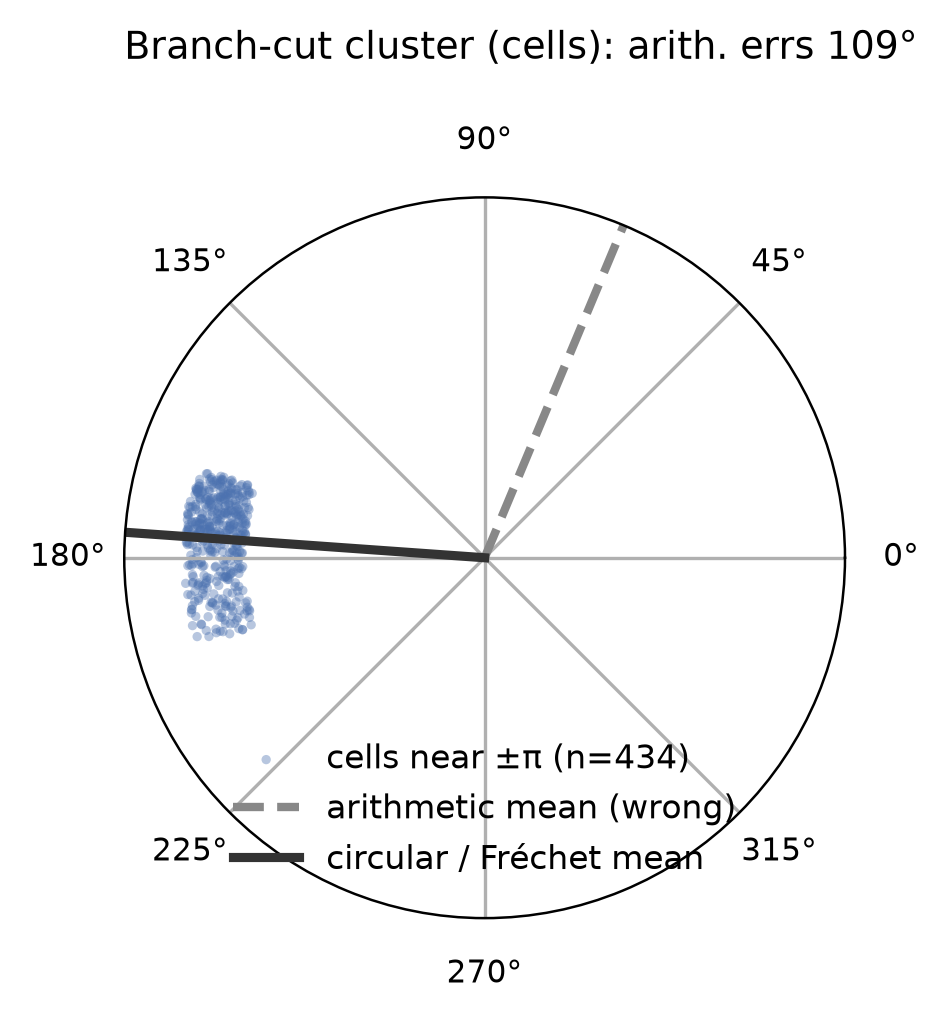
\includegraphics[width=\linewidth]{manifold_branchcut_cells.png}
\caption{Cells: arithmetic mean errs by $109^\circ$; circular/Fr\'echet exact.}
\label{fig:manifold_cells}
\end{subfigure}
\hfill
\begin{subfigure}[t]{0.48\textwidth}
\centering
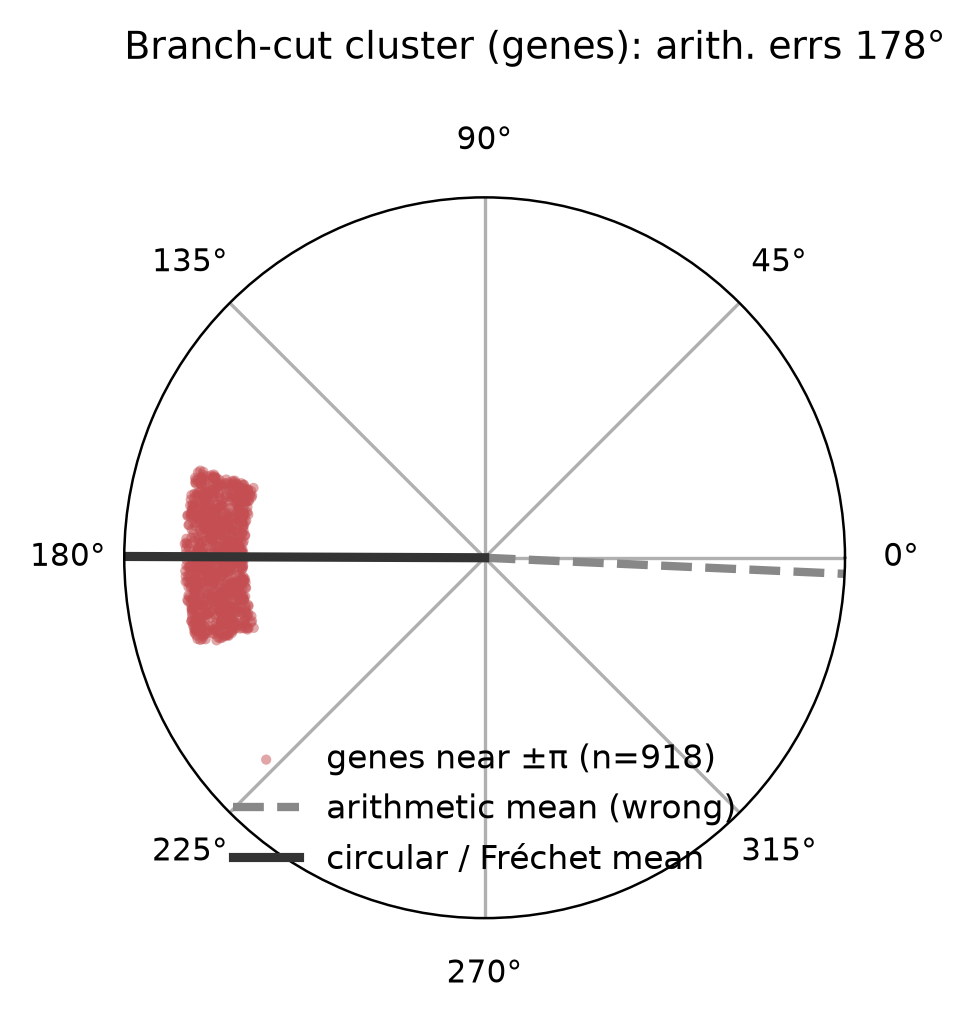
\includegraphics[width=\linewidth]{manifold_branchcut_genes.png}
\caption{Genes: arithmetic mean errs by $178^\circ$; circular/Fr\'echet exact.}
\label{fig:manifold_genes}
\end{subfigure}
\caption{\textbf{The arithmetic mean fails on wrapped phases; the circular mean is exact.} For a cluster straddling the $\pm\pi$ branch cut, the naive arithmetic mean (which ignores wrapping) lands nearly opposite the true centre --- erring by $109^\circ$ for the cell cluster \textbf{(a)} and $178^\circ$ for the gene cluster \textbf{(b)} --- whereas the circular/Fr\'echet mean recovers the correct centroid exactly.}
\label{fig:manifold_means}
\end{figure}

% ================================================================
\subsection{Cell State Tensor Construction and Dynamics}
\label{subsec:r_cst}

\emph{Status: measured on real data (CPTAC UCEC).} We constructed the Cell
State Tensor from the matched CPTAC UCEC RNA and protein phase layers and
tested two claims with the unmodified \texttt{CSTDynamics} and phase-flip
routines at documented defaults. Both fail on this cohort; the verdict is
\emph{does-not-reproduce}, and the failure is informative about the operator's
domain of validity.

\emph{(i) Coherence under Kuramoto evolution (fails).} Under the documented
\texttt{CSTDynamics} evolution ($K = 3$, 300 steps) global coherence
\emph{decreases} from $0.612$ to $0.519$ and phase entropy \emph{increases}
from $3.146$ to $3.277$---the opposite of the predicted rise in coherence and
fall in entropy. Coherence-weighted Kuramoto coupling on two heterogeneous
omics layers drives them apart rather than into a common phase.

\emph{(ii) Phase-flip knockout screen (fails).} Rotating each of the 7{,}083
genes by $\pi$ and ranking by resulting global-coherence loss (verified
bit-identical to the package \texttt{phase\_flip} loop), the top-100 hits
contain \emph{zero} pan-essential genes against a family-level reference
(Hart et al.\ 2015 core-essential + DepMap common-essentials; 249 essentials
present): fold enrichment $0.0\times$, hypergeometric $p = 1.0$, versus a
$3.5\%$ background rate. The top hits (CLIC6, TNXB, SPARCL1, \dots) are
tumour/normal-differential genes, not fitness-essential ones
(Figure~\ref{fig:cst}). Diagnosis: the phasor ``essentiality'' proxy tracks
differential expression magnitude, not genetic dependency, so it cannot stand
in for a CRISPR essentiality screen without a fitness-anchored coupling model.
This is a genuine negative that redirects the knockout-screen design for the
full-scale iteration.

\begin{figure}[!htb]
\centering
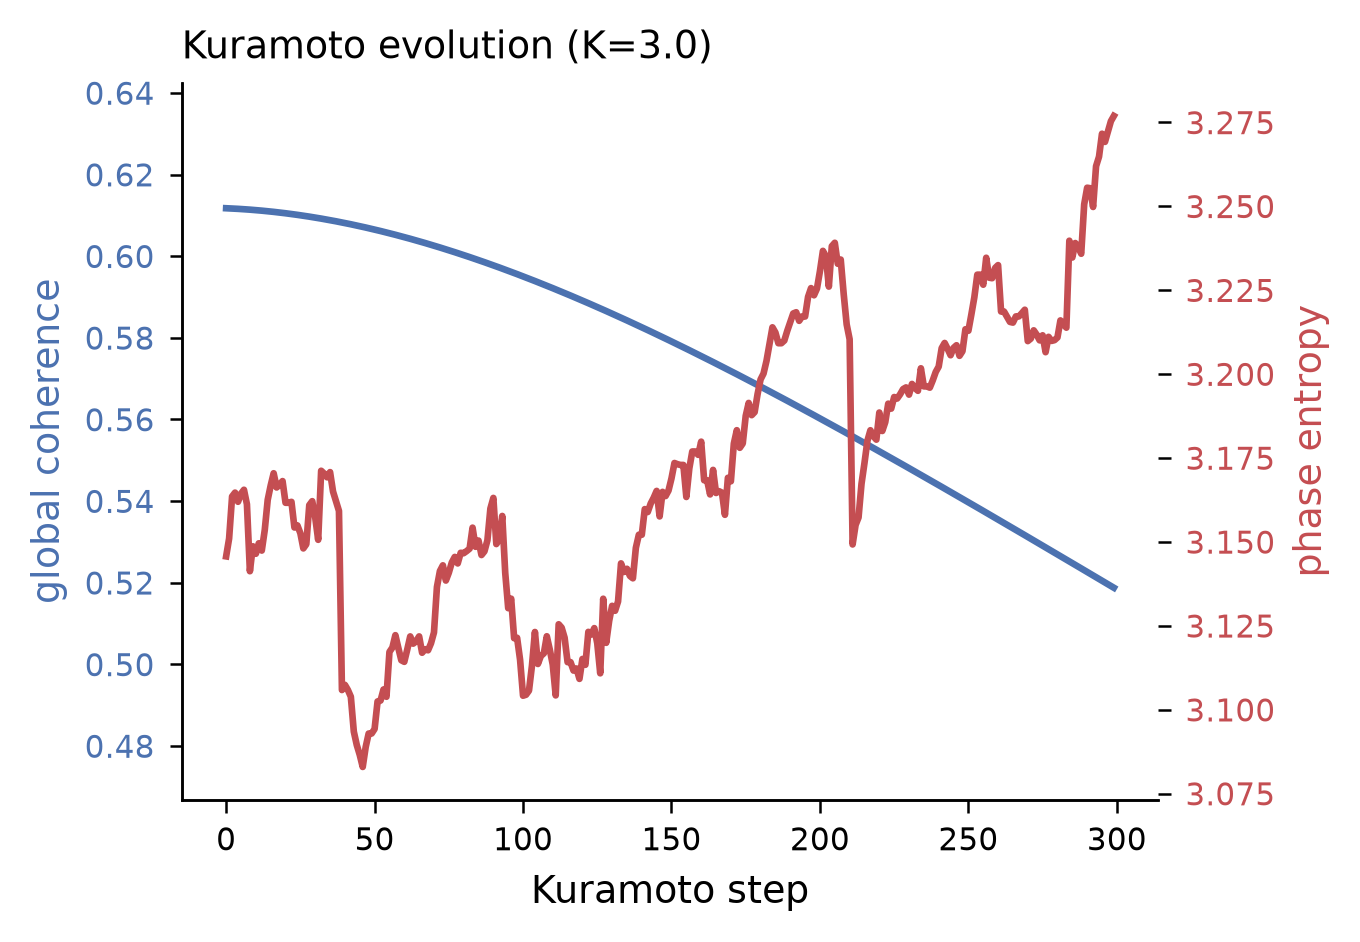
\includegraphics[width=0.62\textwidth]{cst_evolution.png}
\caption{\textbf{Cell State Tensor dynamics run opposite to the claim (real CPTAC UCEC).} Under the documented \texttt{CSTDynamics} Kuramoto evolution ($K=3$, $300$ steps), global coherence \emph{decreases} ($0.61\to0.52$) while phase entropy \emph{increases} ($3.15\to3.28$) --- the opposite of the predicted coherence-increasing convergence. The associated knockout screen is in Figure~\ref{fig:cst_knockout}.}
\label{fig:cst}
\end{figure}

\begin{figure}[!htb]
\centering
\begin{subfigure}[t]{0.48\textwidth}
\centering
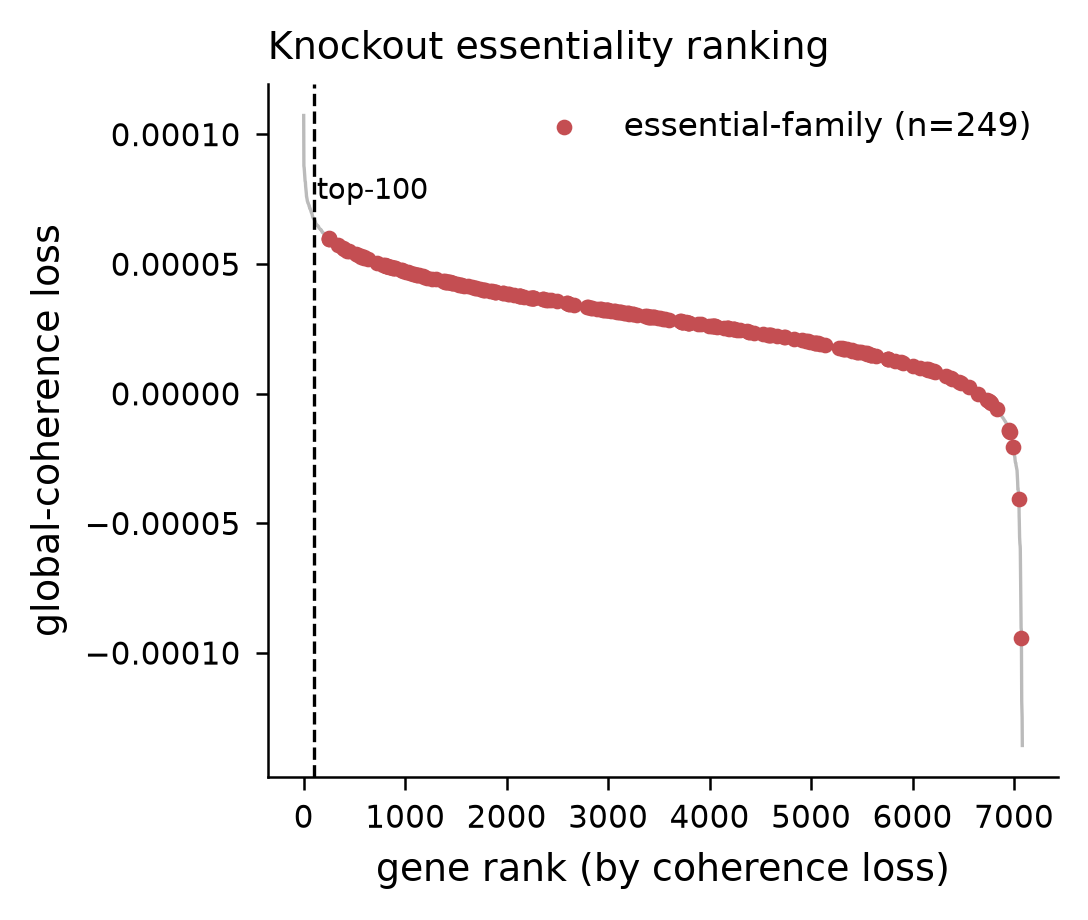
\includegraphics[width=\linewidth]{cst_knockout_rank.png}
\caption{Essential genes are not concentrated at the top of the ranking.}
\label{fig:cst_a}
\end{subfigure}
\hfill
\begin{subfigure}[t]{0.48\textwidth}
\centering
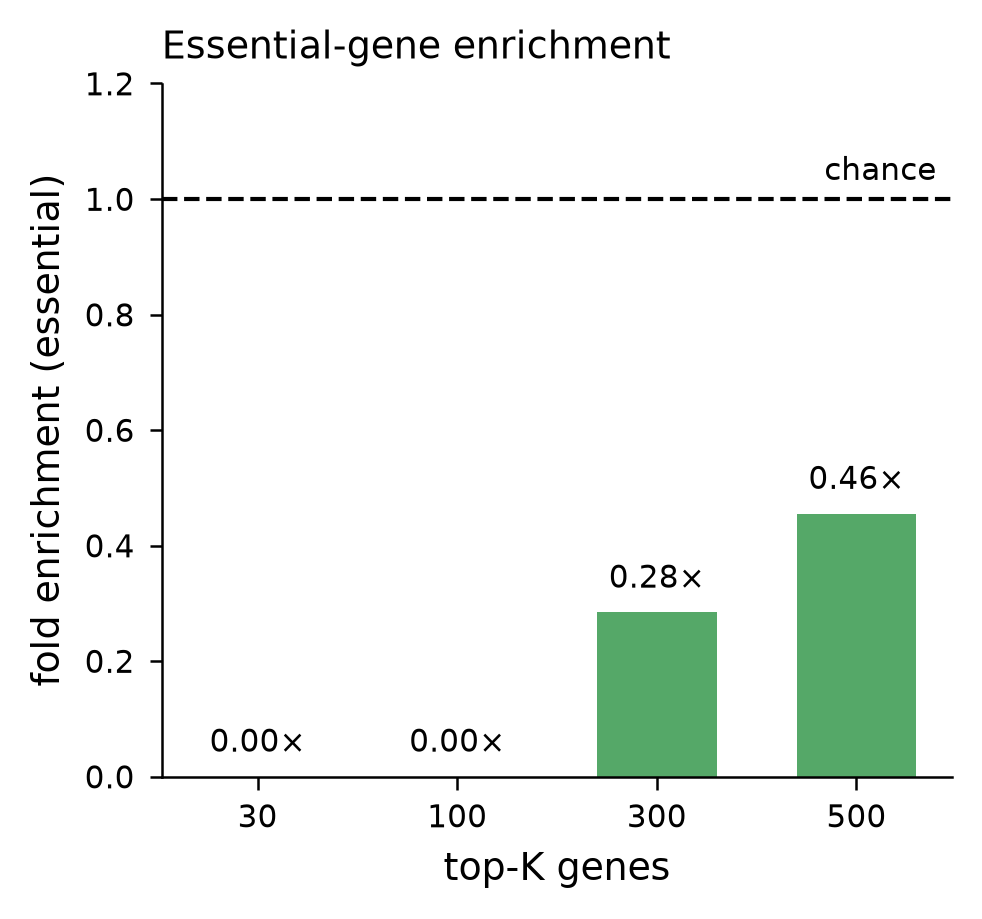
\includegraphics[width=\linewidth]{cst_enrichment.png}
\caption{Essential-gene enrichment is at or below chance at every top-$K$.}
\label{fig:cst_b}
\end{subfigure}
\caption{\textbf{Phase-flip knockout screen recovers no essential-gene signal (real CPTAC UCEC).} \textbf{(a)}~Genes ranked by coherence loss on phase-flip knockout; known essential-family genes (Hart2015\,/\,DepMap) are scattered through the ranking, not concentrated at the top. \textbf{(b)}~Fold enrichment of essentials in the top-$K$ hits is at or below chance for $K\in\{30,100,300,500\}$ (top-100 fold $0\times$, $p=1.0$); the top hits are differential, not essential, genes.}
\label{fig:cst_knockout}
\end{figure}

% ================================================================
\subsection{Time-Resolved CST Profiles on Real Biological Time-Series}
\label{subsec:r_cst_temporal}

\emph{Status: measured on real time-series (GSE293316 cell-cycle pseudotime;
GSE171432 circadian).} The preceding CST results characterise a static
snapshot; here we test the temporal behaviour the framework predicts---that the
CST features $\mathcal{G}_t$ (global coherence), $\mathcal{E}_t$ (phase
entropy), and $R_t$ (state velocity, Eqs.~\ref{eq:cst_coherence}--\ref{eq:cst_velocity})
trace a coherent trajectory as the cell moves through an oscillatory
program---and the Temporal Update Rule (Eq.~\ref{eq:cst_ema}) that stabilises
these estimates. Because per-cell coherence is a dropout artefact on sparse
single-cell data (Section~\ref{subsec:r_encoding}), every single-cell CST here
is \emph{pseudobulked} within its time bin. The verdict is \emph{partial}: the
predicted temporal structure appears clearly when the time axis is densely
sampled, and is sampling-limited when it is not.

\emph{(i) Cell-cycle pseudotime (reproduces).} Ordering 4{,}000 proliferating
REH cells on the continuous cell-cycle angle $\arctan2(\mathrm{G2M},\mathrm{S})$
and pseudobulking into 10 equal-count pseudotime bins ($381$ marker + top-variance
genes), the per-bin CST global coherence rises from $\mathcal{G}=0.370$ in early
G1 (bin~0) to a G2/M peak of $0.845$ (bin~7; net rise $+0.475$) and then crashes
to its minimum $0.262$ at the post-mitotic bin (bin~9), with phase entropy
$\mathcal{E}_t$ anti-correlated to coherence throughout
(Figure~\ref{fig:cst_temporal_cc}). The state velocity $R_t=\|\Delta\phi\|_1/N$
peaks at exactly the two phase boundaries---bin~0 (the cyclic M$\to$G1 wrap) and
bin~4 (G1$\to$S)---identifying the transitions the framework predicts should be
the fastest-moving points of the trajectory. The rise is not strictly monotonic
(a minor dip at bin~3), but the G1-low / G2M-high / post-mitotic-crash arc is
unambiguous. This is a genuine positive: the CST temporal profile recovers
cell-cycle structure directly from real single-cell data.

\emph{(ii) Circadian time (partial, sampling-limited).} On the WT mouse-liver
series (GSE171432; 60 rhythmic genes = 14 core-clock $\cup$ 53 with rhythmicity
score $\ge0.30$) each of the six Zeitgeber times yields a CST whose phase
entropy $\mathcal{E}_t$ oscillates with genuine 24\,h structure---oscillation
amplitude $0.0554$ versus an arrhythmic-gene null mean of $0.0186$
($p<0.001$, peak ZT$18.4$)---but whose coherence trace $\mathcal{G}_t$ does not
clear the null (amplitude $0.0216$ vs.\ null $0.0466$, $p=0.92$;
Figure~\ref{fig:cst_temporal_circ}). Six timepoints sit at the Nyquist floor for
a 24\,h rhythm, the same sampling limit that caps circadian recall at $0.43$ in
Section~\ref{subsec:r_circadian}; the entropy axis carries the temporal signal
that the coherence axis cannot resolve at this density.

\emph{(iii) Temporal update rule (reproduces).} On a noisy 40-step CST
coherence trace the Temporal Update Rule (Eq.~\ref{eq:cst_ema}) behaves as
specified: fixed EMA smoothing ($\lambda=0.85$) cuts trace variance three-fold
($0.0323\to0.0107$) but lags a genuine state transition (tracking error $0.416$
over the transition window). The adaptive-$\lambda$ variant---dropping $\lambda$
to $0.25$ at the four steps where $R_t$ spikes---retains most of the smoothing
(variance $0.0175$) while tracking the same transition roughly three times more
closely (error $0.140$), the responsiveness--stability trade-off the adaptive
rule is designed to make (Figure~\ref{fig:cst_ema}).

\begin{figure}[!htb]
\centering
\begin{subfigure}[t]{0.48\textwidth}
\centering
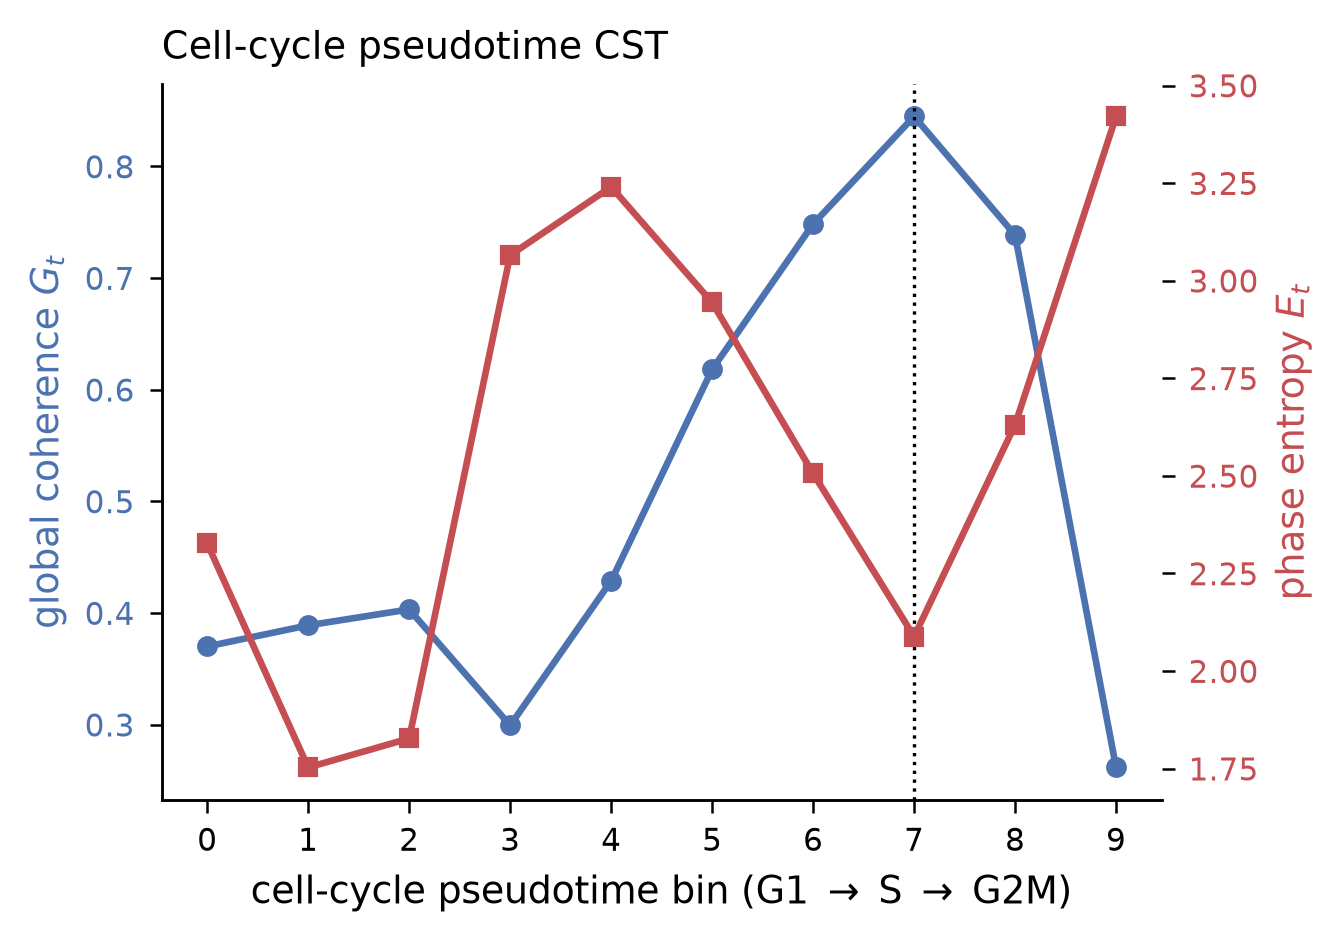
\includegraphics[width=\linewidth]{cst_temporal_cellcycle.png}
\caption{Coherence $\mathcal{G}_t$ rises G1$\to$G2M peak (bin 7), entropy $\mathcal{E}_t$ anti-correlated.}
\label{fig:cst_temporal_cc}
\end{subfigure}
\hfill
\begin{subfigure}[t]{0.48\textwidth}
\centering
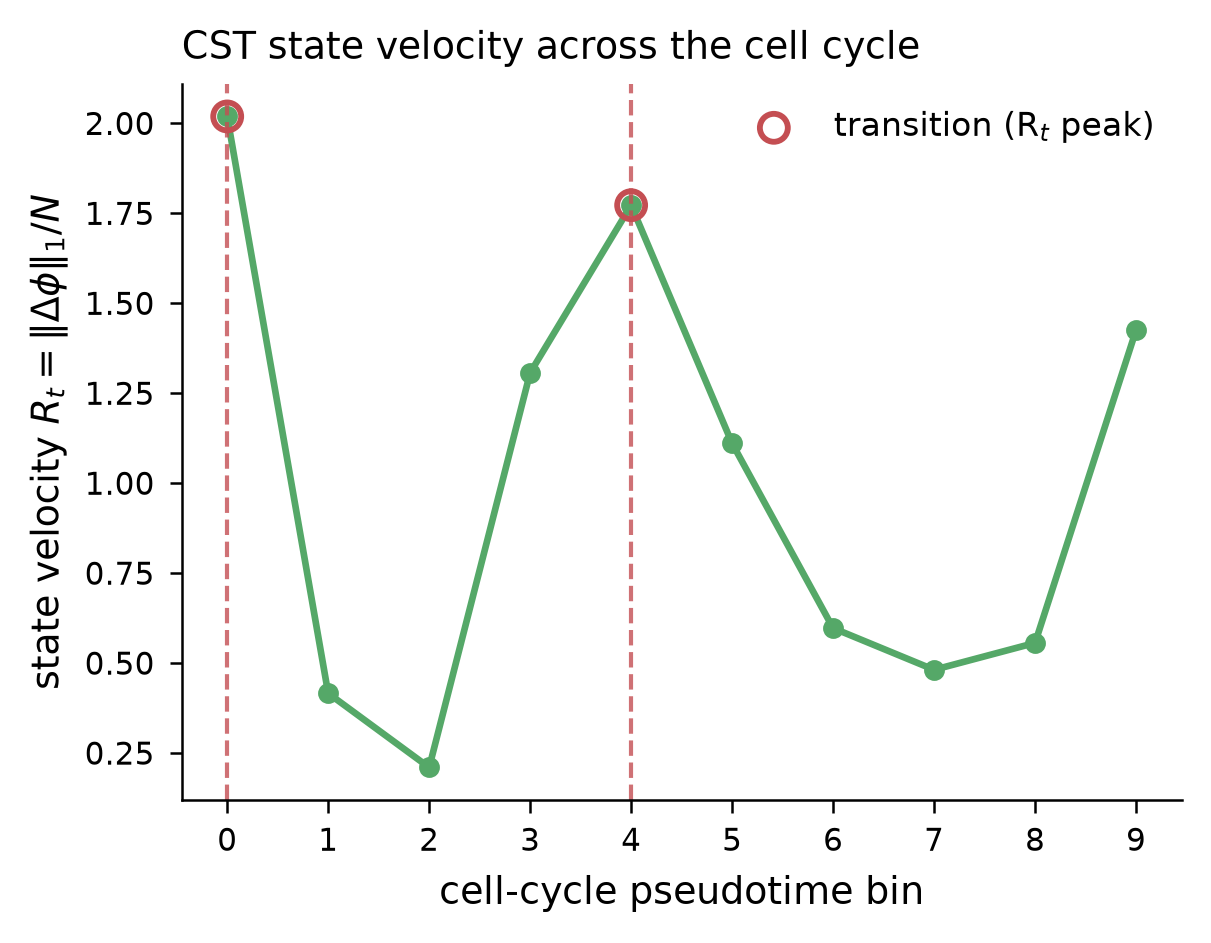
\includegraphics[width=\linewidth]{cst_temporal_velocity.png}
\caption{State velocity $R_t$ peaks at the two cell-cycle phase boundaries.}
\label{fig:cst_temporal_vel}
\end{subfigure}
\caption{\textbf{CST temporal profile reproduces cell-cycle structure (real GSE293316, pseudobulked pseudotime).} \textbf{(a)}~Across 10 pseudotime bins (4{,}000 cells ordered on the continuous cell-cycle angle), CST global coherence $\mathcal{G}_t$ rises from early G1 ($0.370$) to a G2/M peak ($0.845$, bin~7) and crashes post-mitosis ($0.262$, bin~9), with phase entropy $\mathcal{E}_t$ anti-correlated. \textbf{(b)}~State velocity $R_t=\|\Delta\phi\|_1/N$ peaks at exactly the two phase boundaries (the cyclic M$\to$G1 wrap at bin~0 and G1$\to$S at bin~4). Per-bin CSTs are pseudobulked to avoid the single-cell dropout artefact of Section~\ref{subsec:r_encoding}.}
\label{fig:cst_temporal_cc_fig}
\end{figure}

\begin{figure}[!htb]
\centering
\begin{subfigure}[t]{0.48\textwidth}
\centering
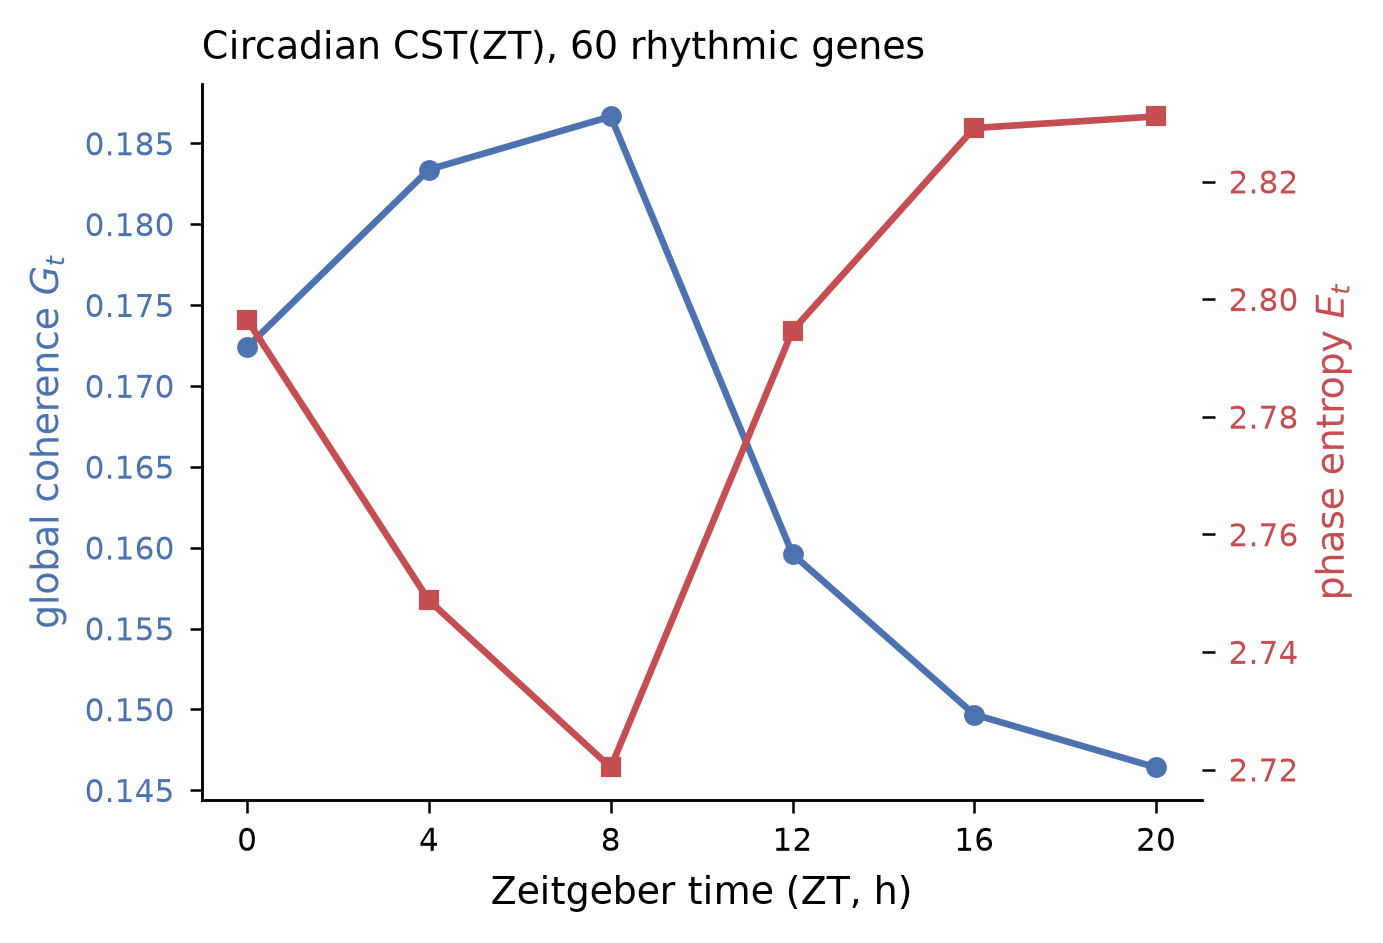
\includegraphics[width=\linewidth]{cst_temporal_circadian.png}
\caption{Circadian CST: entropy oscillates over 24\,h ($p<0.001$); coherence is Nyquist-limited at 6 ZT.}
\label{fig:cst_temporal_circ}
\end{subfigure}
\hfill
\begin{subfigure}[t]{0.48\textwidth}
\centering
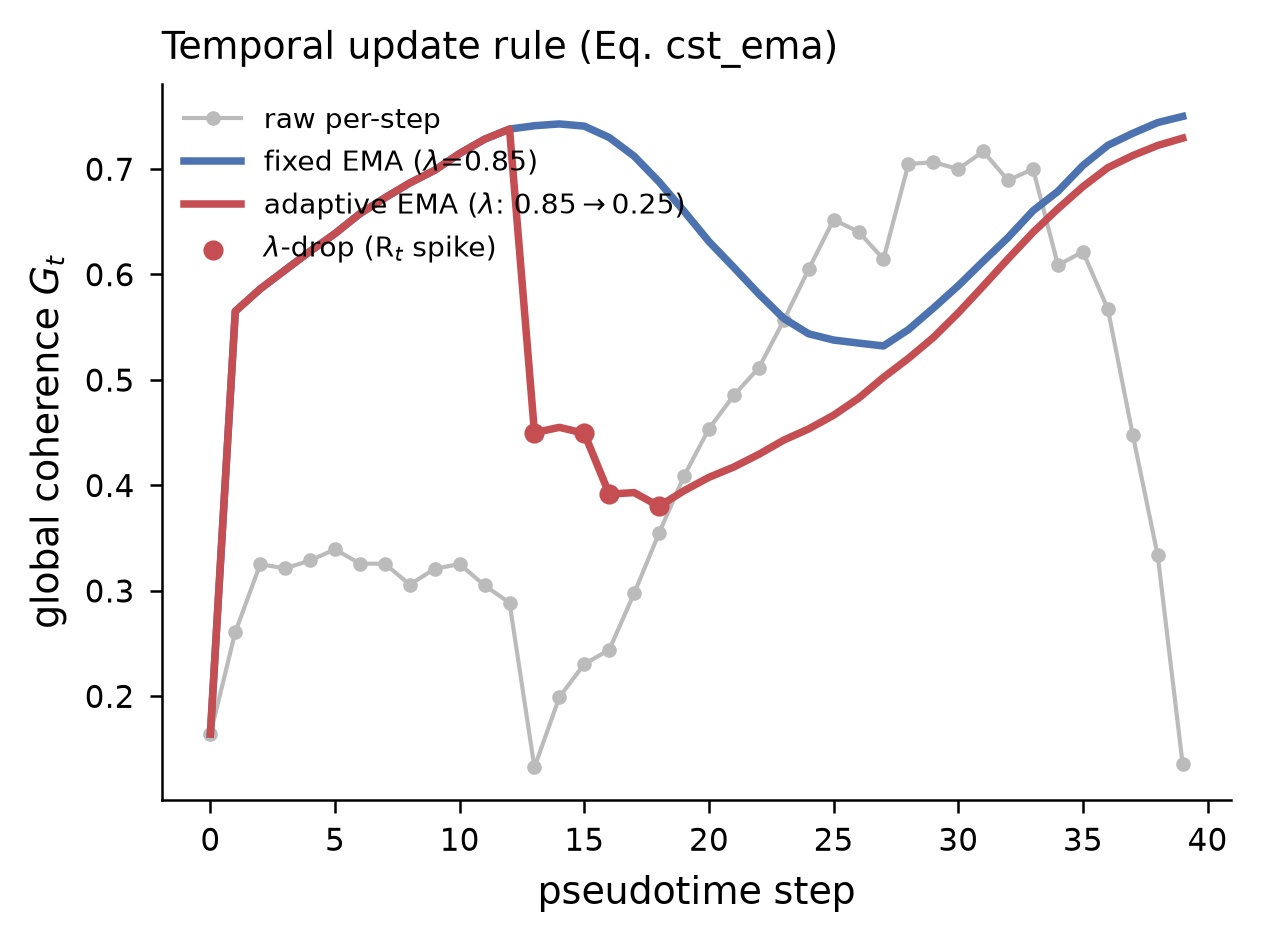
\includegraphics[width=\linewidth]{cst_ema_smoothing.png}
\caption{Temporal update rule: adaptive-$\lambda$ EMA tracks a transition $\sim3\times$ tighter than fixed EMA.}
\label{fig:cst_ema}
\end{subfigure}
\caption{\textbf{Circadian CST profile and the temporal update rule.} \textbf{(a)}~On the WT mouse-liver circadian series (60 rhythmic genes), CST phase entropy $\mathcal{E}_t$ oscillates with genuine 24\,h structure (amplitude $0.0554$ vs.\ arrhythmic null $0.0186$, $p<0.001$), while coherence $\mathcal{G}_t$ does not clear the null at six ZT points---the Nyquist sampling floor that also caps circadian recall in Section~\ref{subsec:r_circadian}. \textbf{(b)}~The Temporal Update Rule (Eq.~\ref{eq:cst_ema}) on a noisy coherence trace: fixed EMA ($\lambda=0.85$) cuts variance three-fold but lags a state transition (error $0.416$); adaptive-$\lambda$ (dropping to $0.25$ at $R_t$ spikes, marked) keeps the smoothing yet tracks the transition $\sim3\times$ more closely (error $0.140$).}
\label{fig:cst_temporal_ema_fig}
\end{figure}

% ================================================================
\subsection{Tensor-Network Factorization and Uncertainty of the CST}
\label{subsec:r_cst_tn}

\emph{Status: measured on real data (CPTAC UCEC).} We tested the tensor-network
(MPS/tensor-train) factorization the framework proposes for compact CST storage
and online updates (Eq.~\ref{eq:cst_mps}), together with the uncertainty-aware
CST (Section~\ref{sec:cst}). The verdict is \emph{partial}, and the boundary is
informative: tensor-train does not compress a single CST snapshot, but it does
amortize storage across a growing history. (All tensor-train decompositions use
a real/imaginary-stacked representation of the complex CST; \texttt{tensorly}
$0.9.0$'s complex TT-SVD is numerically unreliable---its reconstruction error
grows with bond dimension---so the complex tensor is split into real and
imaginary channels before decomposition, as noted in the Methods.)

\emph{(i) A single CST is not low-rank (does-not-reproduce).} The gene-resolved
CPTAC CST ($7{,}083$ genes $\times\,2$ modalities $\times\,109$ samples) has a
high-entropy gene-mode spectrum: rank $50$ captures only $50\%$ of the spectral
energy and rank $150$ reaches $86\%$ (full rank $218$;
Figure~\ref{fig:cst_tt_spectrum}). Consequently the tensor-train never reaches
even $10\%$ reconstruction error at any bond dimension---the best achieved is
$65\%$ error at $3.2\times$ compression (bond $128$), and pushing compression
above $\sim3\times$ costs more than $65\%$ error
(Figure~\ref{fig:cst_tt_comp}). The regulatory axis carries genuinely
high-dimensional inter-gene structure that no small bond dimension captures, so
Eq.~\ref{eq:cst_mps} does not deliver useful single-snapshot compression on this
real CST.

\emph{(ii) CST history storage is sublinear (reproduces).} The streaming-storage
motivation for the factorization holds at the history level. Stacking CST
snapshots into a growing 4-D history tensor ($L\times R\times T\times H$), dense
storage grows linearly in history length $L$ while the tensor-train's
history-axis bond saturates, so TT storage grows sublinearly: at fixed bond $40$
the compression ratio rises from $2.7\times$ at $L=1$ to $5.1\times$ at $L=64$
(Figure~\ref{fig:cst_tt_storage}). Tensor-train amortizes the redundancy shared
\emph{across} snapshots even though it cannot compress any single one; a full
re-decomposition (a proxy for the rank-adaptive online update) costs on the
order of a second at $L=64$, feasible for periodic rather than per-cell updates.

\emph{(iii) Uncertainty is heterogeneity, not dropout (informative negative).}
Bootstrap-resampling the samples $B=40$ times and rebuilding the CST gives a
per-entry circular variance (Eq.~\ref{eq:cst_uncertainty}) that is high
(mean $0.80$) and---contrary to the manuscript hypothesis that CST uncertainty
is dropout-driven---essentially uncorrelated with expression level (Spearman
$\rho=0.08$, flat across expression quintiles;
Figure~\ref{fig:cst_uncertainty}). On this matched bulk multi-omics cohort the
CST's uncertainty reflects genuine inter-sample biological heterogeneity rather
than measurement dropout, which refines where the dropout-flagging use of
$\boldsymbol{\Sigma}_t$ applies.

\begin{figure}[!htb]
\centering
\begin{subfigure}[t]{0.48\textwidth}
\centering
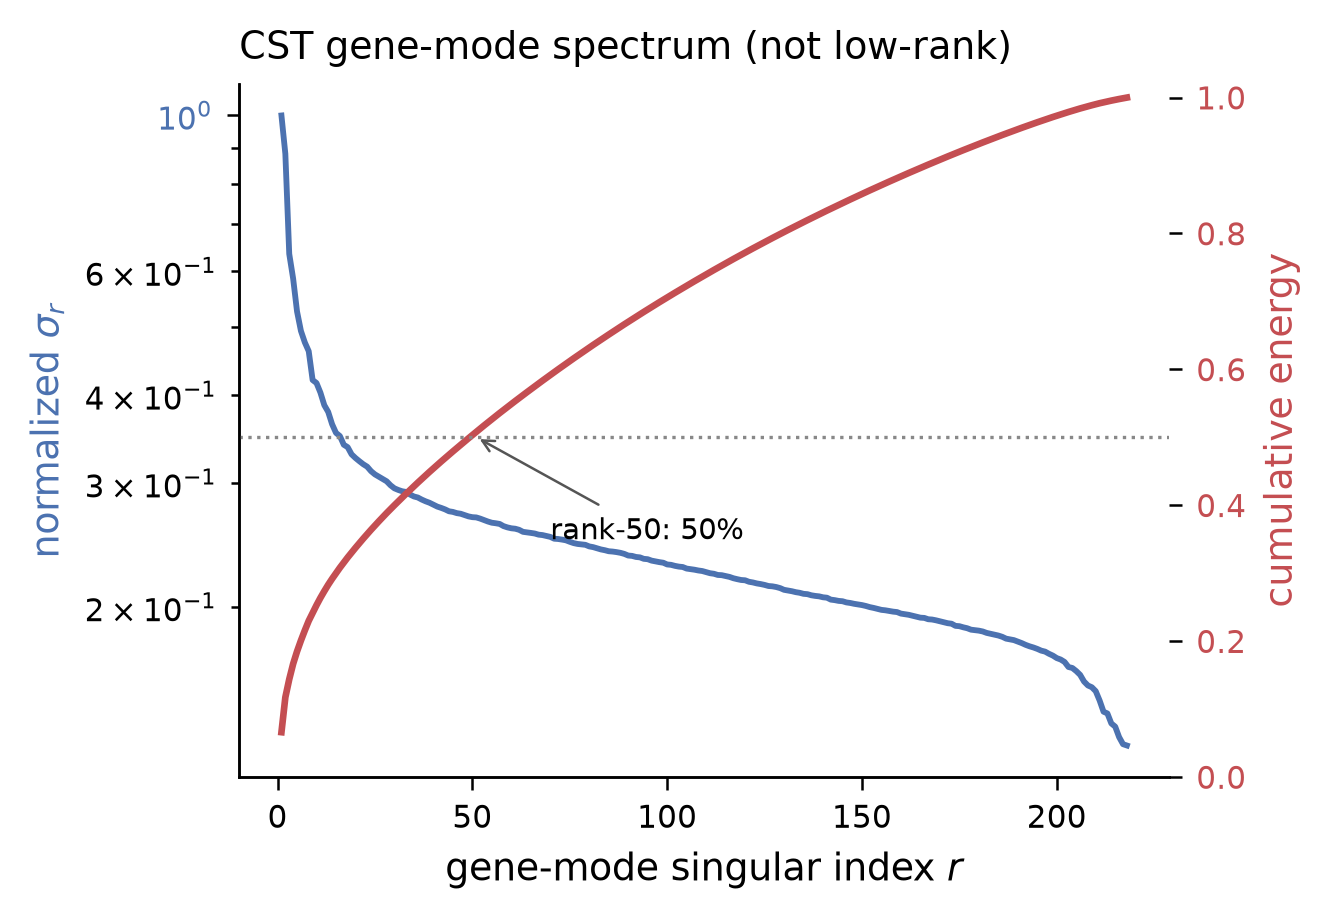
\includegraphics[width=\linewidth]{cst_tt_energy_spectrum.png}
\caption{Gene-mode SVD spectrum: rank-50 is only $50\%$ energy---the CST is not low-rank.}
\label{fig:cst_tt_spectrum}
\end{subfigure}
\hfill
\begin{subfigure}[t]{0.48\textwidth}
\centering
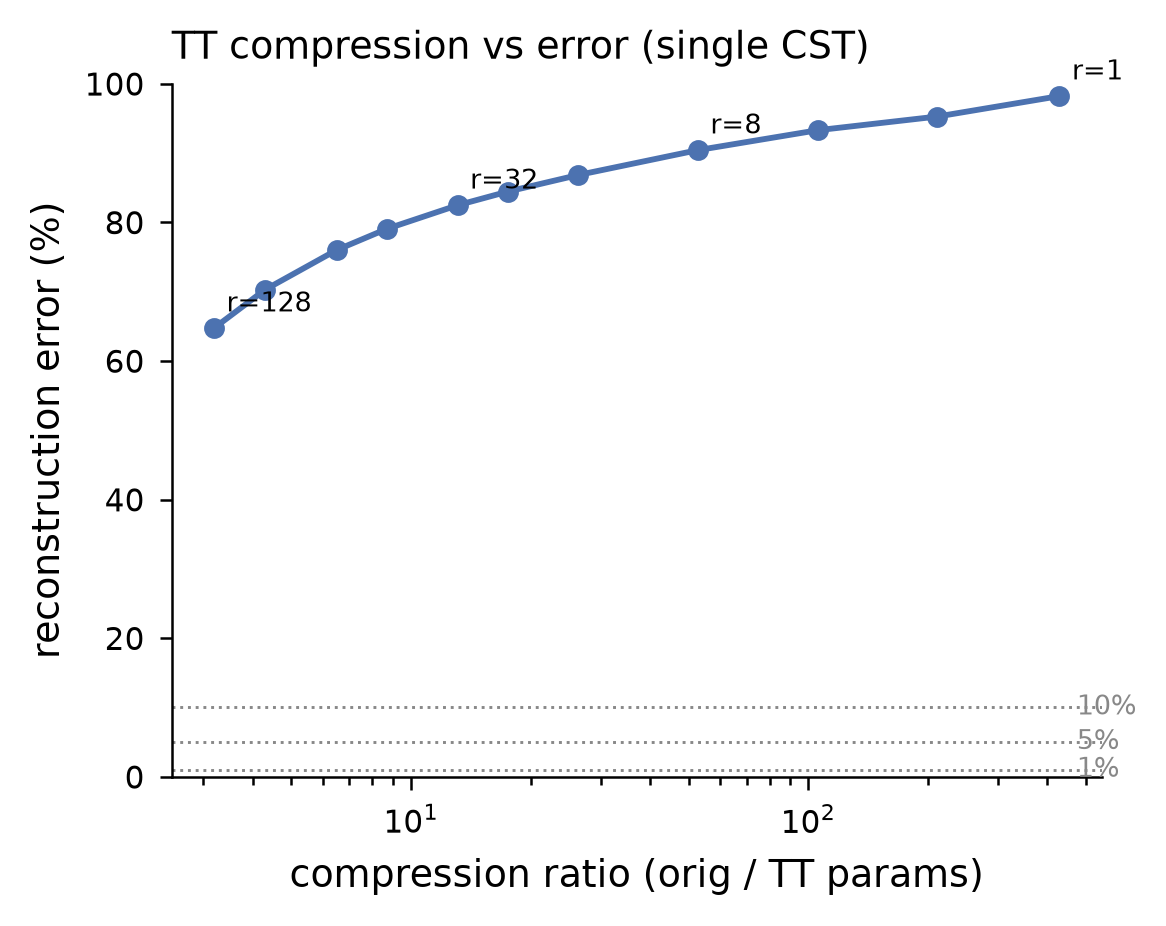
\includegraphics[width=\linewidth]{cst_tt_compression_error.png}
\caption{TT compression vs.\ error: never below $10\%$; best $65\%$ error at $3.2\times$.}
\label{fig:cst_tt_comp}
\end{subfigure}
\caption{\textbf{Tensor-train does not compress a single real CST (CPTAC UCEC).} \textbf{(a)}~The gene-mode singular-value spectrum is high-entropy---rank $50$ captures $50\%$ and rank $150$ captures $86\%$ of the energy (full rank $218$). \textbf{(b)}~Across the bond-dimension sweep the tensor-train reconstruction error never falls below $10\%$ (dotted reference lines at $10/5/1\%$); the best operating point is $65\%$ error at $3.2\times$ compression. The regulatory axis is genuinely high-dimensional.}
\label{fig:cst_tt_single_fig}
\end{figure}

\begin{figure}[!htb]
\centering
\begin{subfigure}[t]{0.48\textwidth}
\centering
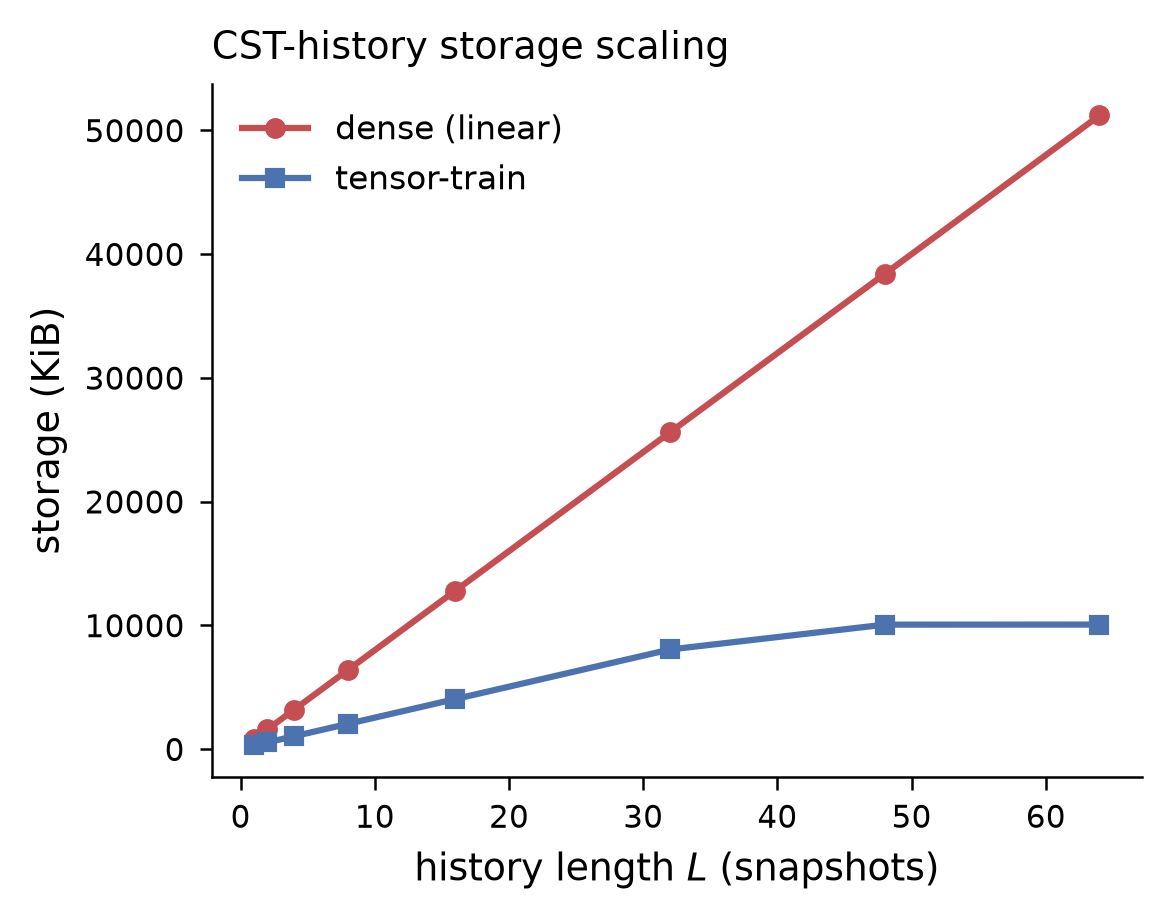
\includegraphics[width=\linewidth]{cst_tt_storage_scaling.png}
\caption{History storage: dense grows linearly in $L$, tensor-train sublinearly ($2.7\times\!\to\!5.1\times$).}
\label{fig:cst_tt_storage}
\end{subfigure}
\hfill
\begin{subfigure}[t]{0.48\textwidth}
\centering
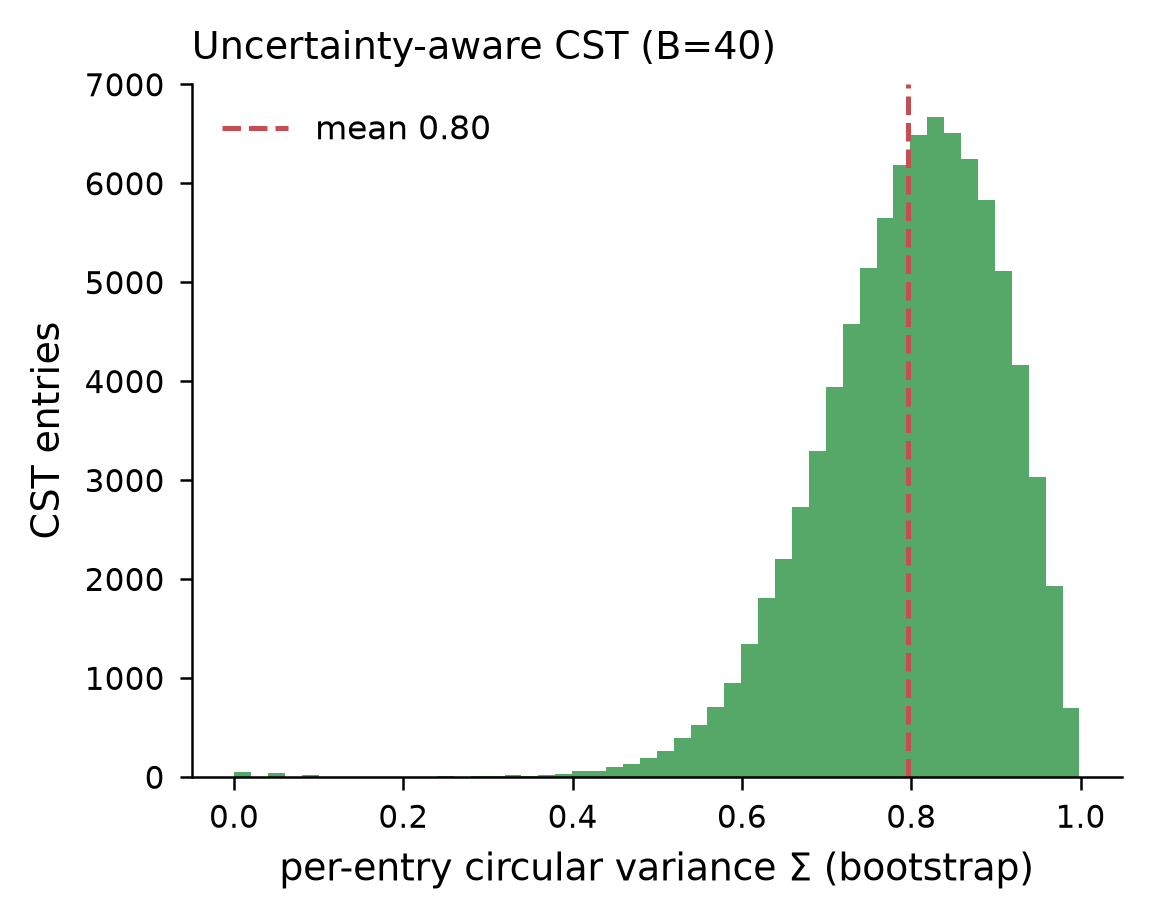
\includegraphics[width=\linewidth]{cst_uncertainty.png}
\caption{Bootstrap per-entry uncertainty (mean $0.80$), uncorrelated with expression ($\rho=0.08$).}
\label{fig:cst_uncertainty}
\end{subfigure}
\caption{\textbf{CST-history storage scaling and uncertainty (real CPTAC UCEC).} \textbf{(a)}~Stacking CST snapshots into a growing history tensor, dense storage grows linearly in history length $L$ while tensor-train storage grows sublinearly (compression $2.7\times$ at $L=1$ to $5.1\times$ at $L=64$, fixed bond $40$)---the factorization amortizes cross-snapshot redundancy. \textbf{(b)}~Per-entry bootstrap circular variance ($B=40$) is high (mean $0.80$) and essentially independent of expression level (Spearman $\rho=0.08$), so the CST's uncertainty on this bulk cohort reflects biological heterogeneity, not measurement dropout.}
\label{fig:cst_tn_hist_fig}
\end{figure}

% ================================================================
\subsection{A Pathway Atlas Roots the Regulatory Axis and Makes the CST Compressible}
\label{subsec:r_cst_pathway}

\emph{Status: partial (real CPTAC UCEC RNA\,+\,protein). Rooting the regulatory
axis in a pathway atlas reproduces low-rank behaviour on that axis, but not for
the full tensor.}

The tensor-network result above (Section~\ref{subsec:r_cst_tn}) found that the
flat gene-resolved CST is not low-rank: its gene-mode spectrum needs rank~50
for half the energy. That is a property of an \emph{unstructured} regulatory
axis---a flat list of $7083$ genes. Section~\ref{subsec:cst_measured} argued
that biology supplies the missing structure through pathways, exactly as an
anatomical atlas supplies structure to a brain tensor's region axis. We test
that claim directly on the same real CPTAC UCEC cohort (RNA\,+\,protein,
$109$ samples), building a pathway-aggregated CST of shape
$50\times2\times109$ ($50$ MSigDB Hallmark programs $\times$ two modalities
$\times$ samples), each pathway carrying the circular-mean phasor of its
member genes. The atlas covers $2405$ of the $7083$ co-observed genes
($34\%$); we report the fair, per-component comparison of captured energy so
the result does not merely restate the $7083\!\rightarrow\!50$ dimensionality
reduction.

Imposing pathway structure collapses the regulatory spectrum
(Fig.~\ref{fig:cst_pathway_spectrum}). A \emph{single} regulatory component of
the pathway CST captures $52.5\%$ of the tensor's energy, and $14$ components
reach $90\%$; the flat-gene CST needs rank~$50$ for $50\%$ and rank~$150$ for
$86\%$ (Section~\ref{subsec:r_cst_tn}), with its leading component capturing
only $6.6\%$. In other words, pathway structure achieves in one component what
the flat gene axis needs about fifty to match---the qualitative signature of
the region-aggregated regime that makes a brain tensor low-rank. The most
phase-coherent Hallmark programs across the cohort
(Fig.~\ref{fig:cst_pathway_coherence}) are proliferation-linked
(\textsc{e2f\_targets}, \textsc{myc\_targets\_v1/v2}, \textsc{g2m\_checkpoint})
together with \textsc{oxidative\_phosphorylation}, while immune and
xenobiotic-metabolism programs are least coherent---a biologically
interpretable readout consistent with proliferation being the dominant
coordinated axis in endometrial carcinoma, and the direct analogue of reading
structure off a brain atlas's regions.

The verdict is \emph{partial} because the collapse is confined to the
regulatory axis. A full CP decomposition of the pathway CST still does not
reach the low-rank point of a genuinely low-dimensional tensor: its CP-rank-3
reconstruction error is $62.3\%$ (versus $94.6\%$ for the flat-gene CST, but
far from the few-percent regime attainable when all three axes are structured)
(Fig.~\ref{fig:cst_pathway_cp}). The reason is structural and honest, not an
atlas deficiency. CPTAC UCEC is a patient \emph{cohort}, so the third axis is
$109$ heterogeneous tumours rather than a low-dimensional time or frequency
axis; that axis alone needs rank~$17$ for $90\%$ of its energy, which bounds
how well any CP-rank-3 set of shared sample loadings can reconstruct the tensor.
Full-tensor compressibility of the CST is therefore expected to require a
structured third axis---matched multi-omics \emph{time series}---which the
pathway atlas cannot supply on its own. The atlas does what it should: it makes
the regulatory axis interpretable and low-rank, the piece BioPhasor most needed
to stop treating genes as an unstructured bag.

\begin{figure}[t]
\centering
\begin{subfigure}[t]{0.48\textwidth}
\centering
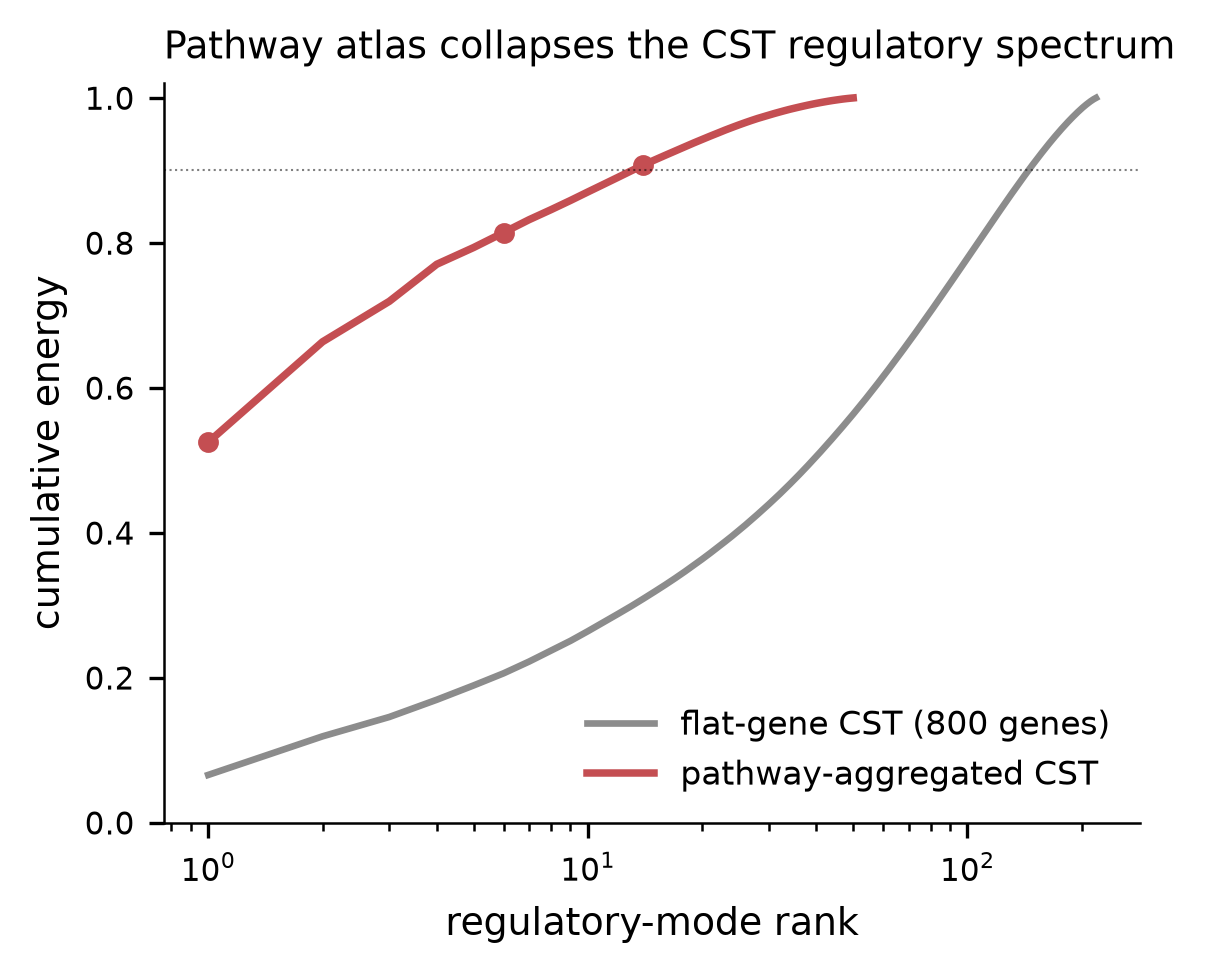
\includegraphics[width=\linewidth]{cst_pathway_spectrum.png}
\caption{Regulatory-mode cumulative energy: the pathway-aggregated CST reaches
$52.5\%$ at rank~$1$; the flat-gene CST needs $\sim\!50$ components for $50\%$.}
\label{fig:cst_pathway_spectrum}
\end{subfigure}\hfill
\begin{subfigure}[t]{0.48\textwidth}
\centering
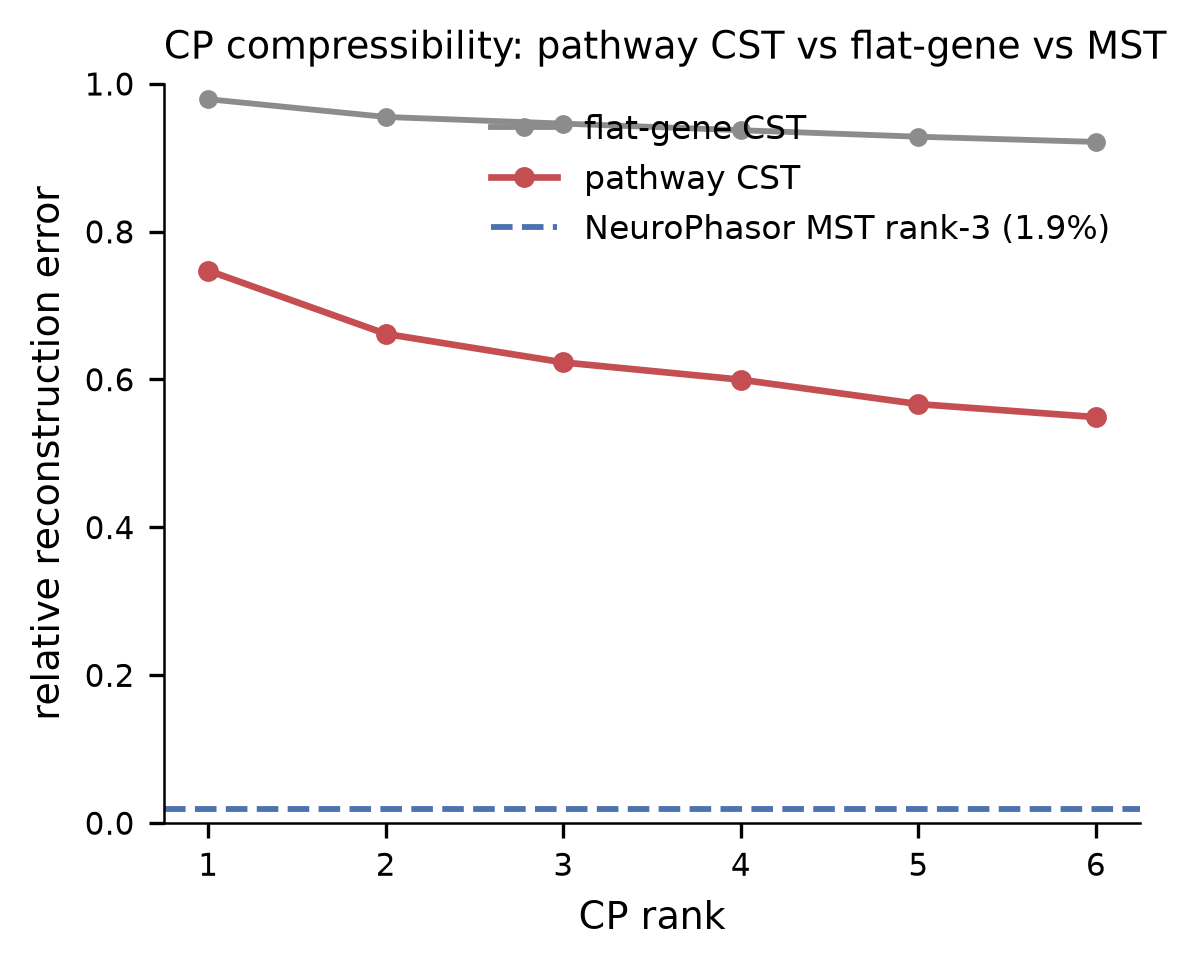
\includegraphics[width=\linewidth]{cst_pathway_cp_error.png}
\caption{CP reconstruction error vs rank: the pathway CST ($62\%$ at rank~3)
beats flat-gene ($95\%$) but does not reach the few-percent regime of a fully
structured tensor (dashed reference).}
\label{fig:cst_pathway_cp}
\end{subfigure}
\caption{\textbf{A pathway atlas roots the CST regulatory axis (real CPTAC
UCEC).} Aggregating $7083$ genes onto $50$ MSigDB Hallmark programs supplies the
regulatory axis with biological structure---the multi-omics counterpart of an
anatomical atlas. \textbf{(a)}~This collapses the regulatory-mode spectrum
toward the low-rank regime; \textbf{(b)}~full-tensor CP compressibility remains
partial because the cohort's sample axis carries irreducible tumour
heterogeneity (see text).}
\label{fig:cst_pathway_fig}
\end{figure}

\begin{figure}[t]
\centering
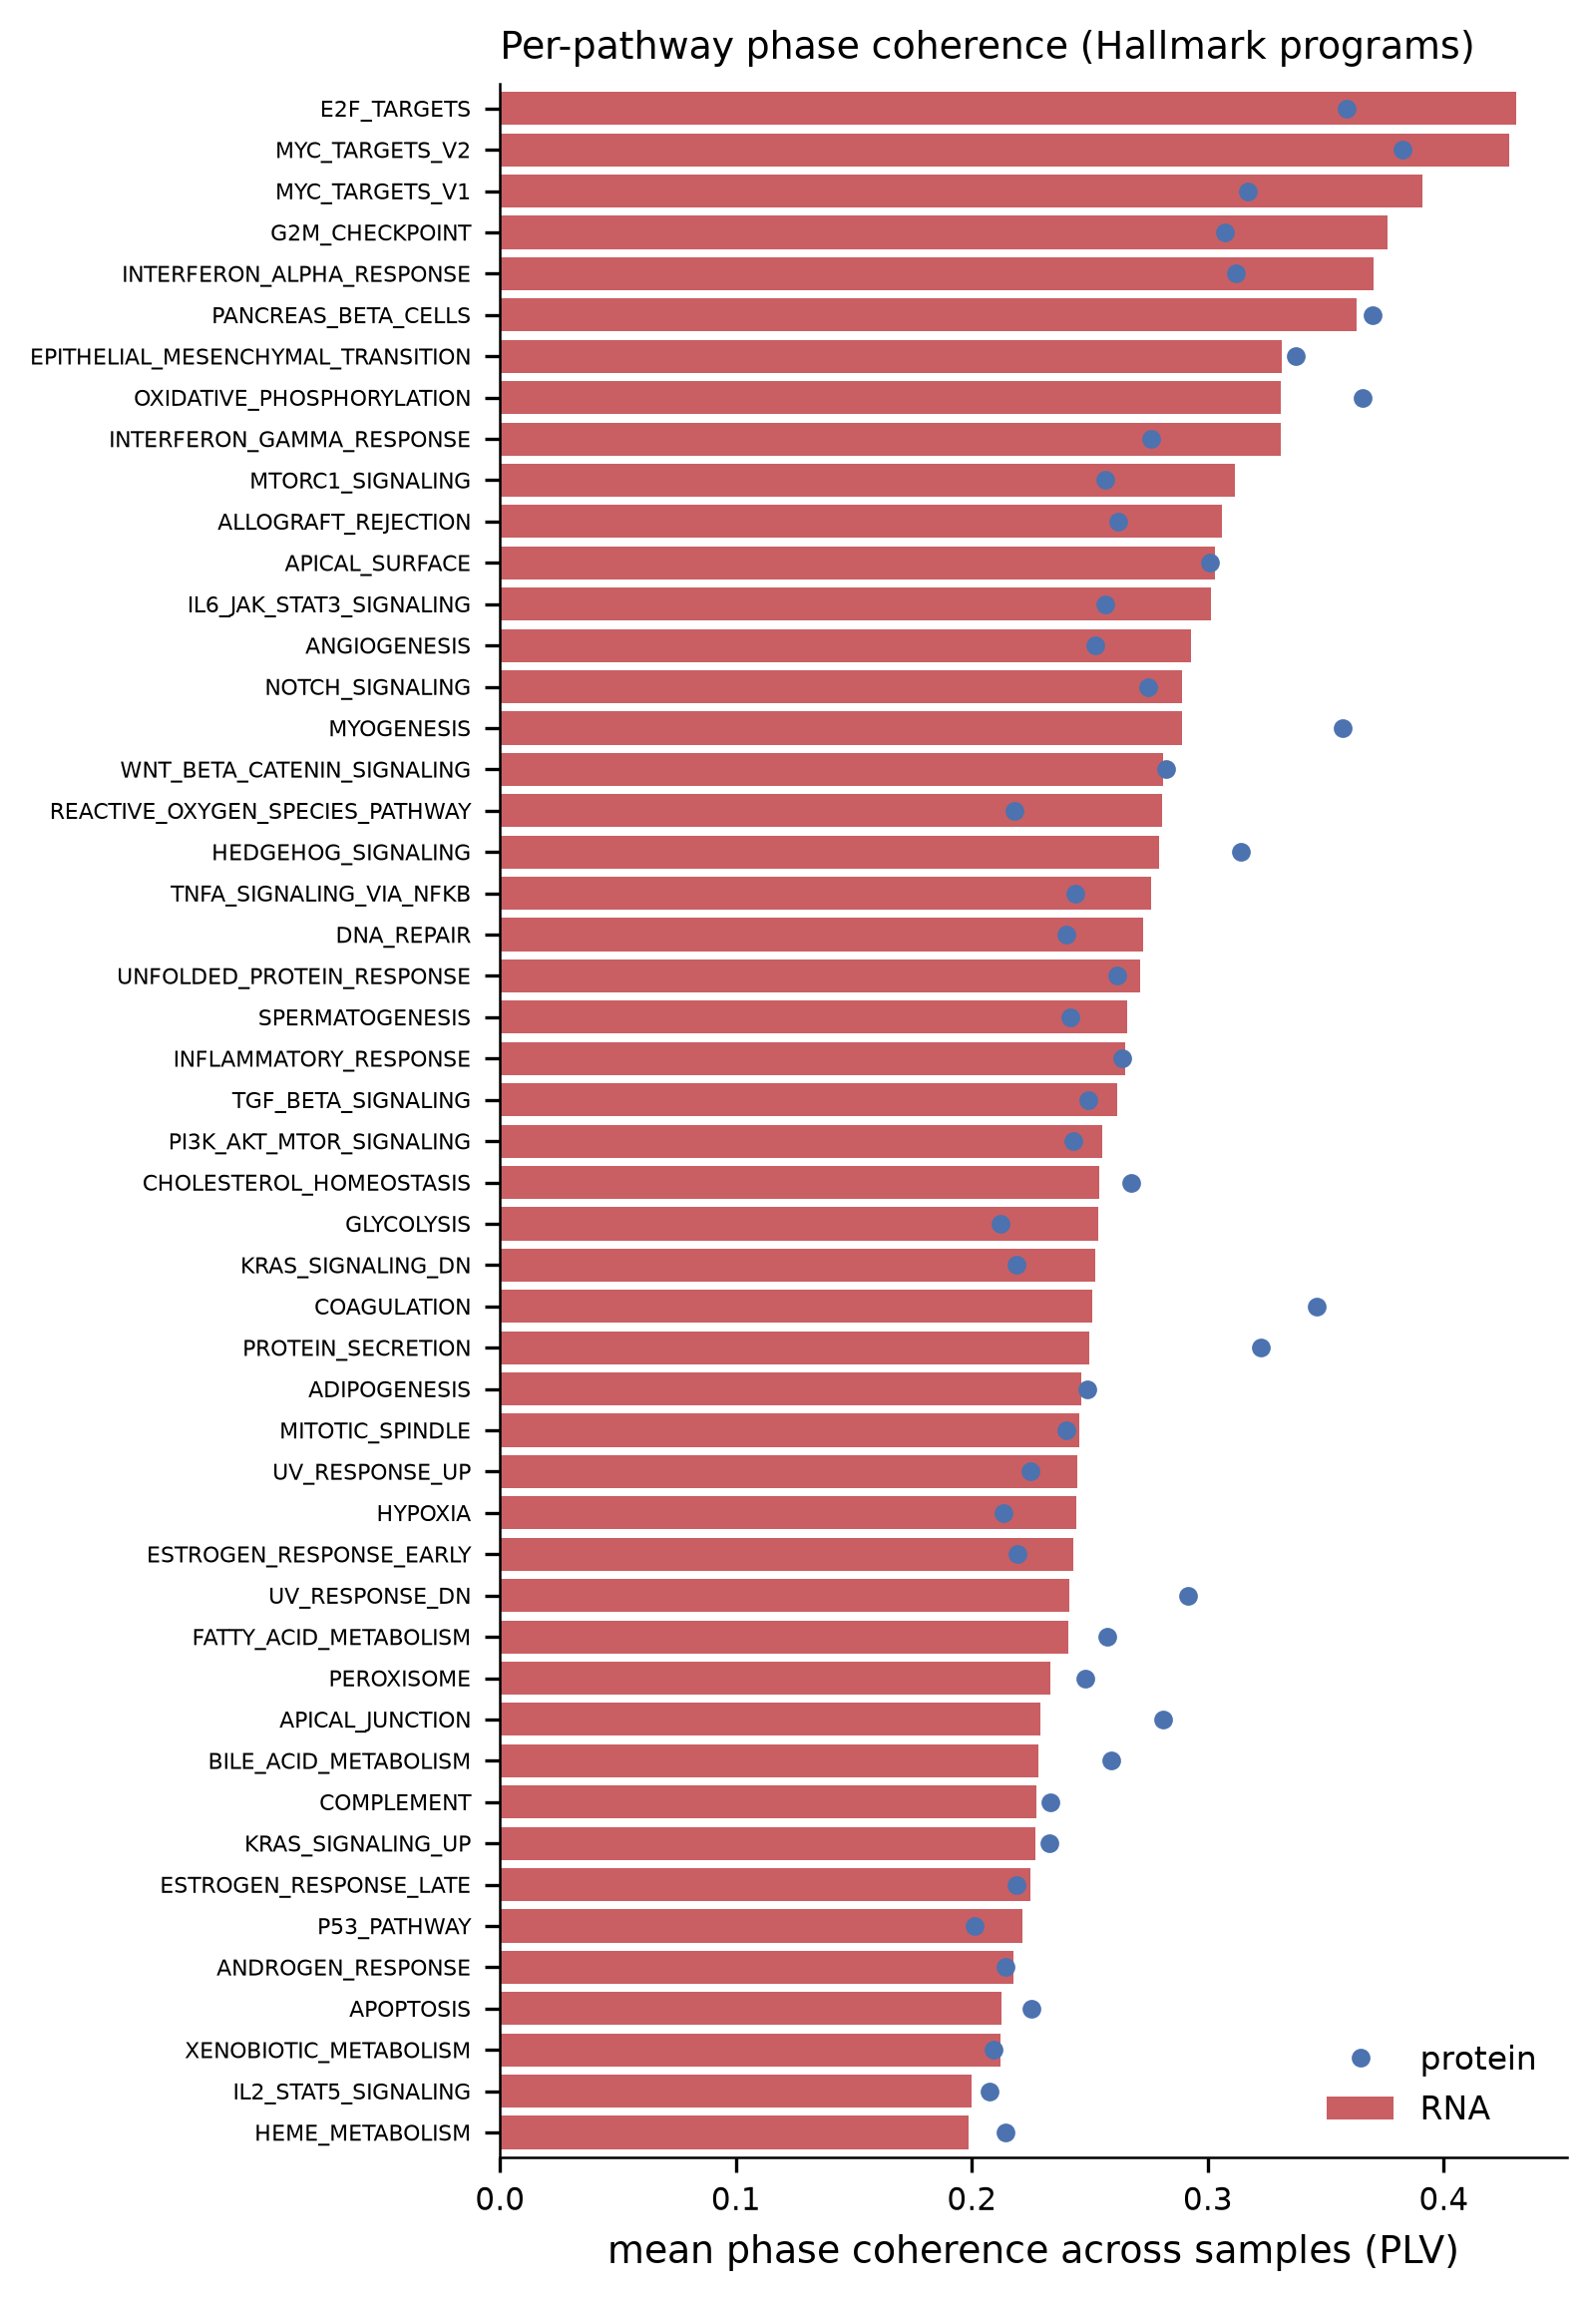
\includegraphics[width=0.62\linewidth]{cst_pathway_coherence.png}
\caption{\textbf{Per-pathway phase coherence across the UCEC cohort.} Mean
across-sample phase coherence (PLV) of each Hallmark program, RNA (bars) and
protein (points). Proliferation programs (\textsc{e2f}, \textsc{myc},
\textsc{g2m}) and \textsc{oxidative\_phosphorylation} are the most phase-coherent;
immune and xenobiotic-metabolism programs the least---an interpretable
biological readout off the pathway atlas, analogous to reading structure off a
brain atlas's regions. Protein coherence is generally lower than RNA, consistent
with post-transcriptional buffering.}
\label{fig:cst_pathway_coherence}
\end{figure}

% ================================================================
\subsection{Illustrative Application: Cross-Modal Phase Coupling Along the Central Dogma}
\label{subsec:r_cst_pac}

\emph{Status: reproduces (real CPTAC UCEC RNA\,+\,protein).}

As a final illustration of what the modality axis of the CST makes measurable, we
ask whether, across the $109$ CPTAC UCEC patients, the \emph{phase} of a gene's
mRNA phasor organises the \emph{amplitude} of its protein---a multi-omics analogue
of cross-frequency phase--amplitude coupling \citep{scherer2022} transposed onto
the central dogma. For each gene we bin the across-sample mRNA phase into $K=9$
bins, take the mean protein amplitude per bin, and score the non-uniformity with a
Tort-style modulation index (MI); the null circularly permutes the sample
correspondence between modalities ($N=10{,}000$ permutations). The coupling is
present and highly significant: the aggregate per-gene MI lies far outside the
null ($z=180$, $\sim\!2.3\times$ the null mean; pooled circular--linear
$r=0.295$, $95\%$ CI $[0.291,0.299]$), $70.4\%$ of $7{,}083$ genes remain
significant at BH-FDR $<0.05$, and the effect is strongly tumour-specific
($r=0.295$ across $95$ tumours vs.\ $0.029$ across $14$ normals;
Fig.~\ref{fig:cst_pac_comod}). At the cohort level the coupling is
\emph{symmetric}---the reverse protein$\to$mRNA coupling ($r=0.285$) is nearly as
strong as the forward direction---so the data establish a real, tumour-specific
cross-modal coupling but do not, from a cross-sectional cohort, demonstrate a
directional mRNA$\to$protein flow; we read it as the signature of pervasive
post-transcriptional regulation \citep{srivastava2022}.

This vignette demonstrates that the CST modality axis is a genuine, non-neural
BioPhasor observable equipped with a proper surrogate null---the property that
makes the CST a multi-omics object rather than a phasor tensor by analogy. A full
treatment of this tumour-specific coupling as a use case of the BioPhasor
formulation---directionality tests, biological module structure, and clinical
stratification---is developed in a dedicated study; here it serves only to
exercise the platform's phase--amplitude-coupling capability end-to-end on real
matched multi-omics data.

\begin{figure*}[t]
\centering
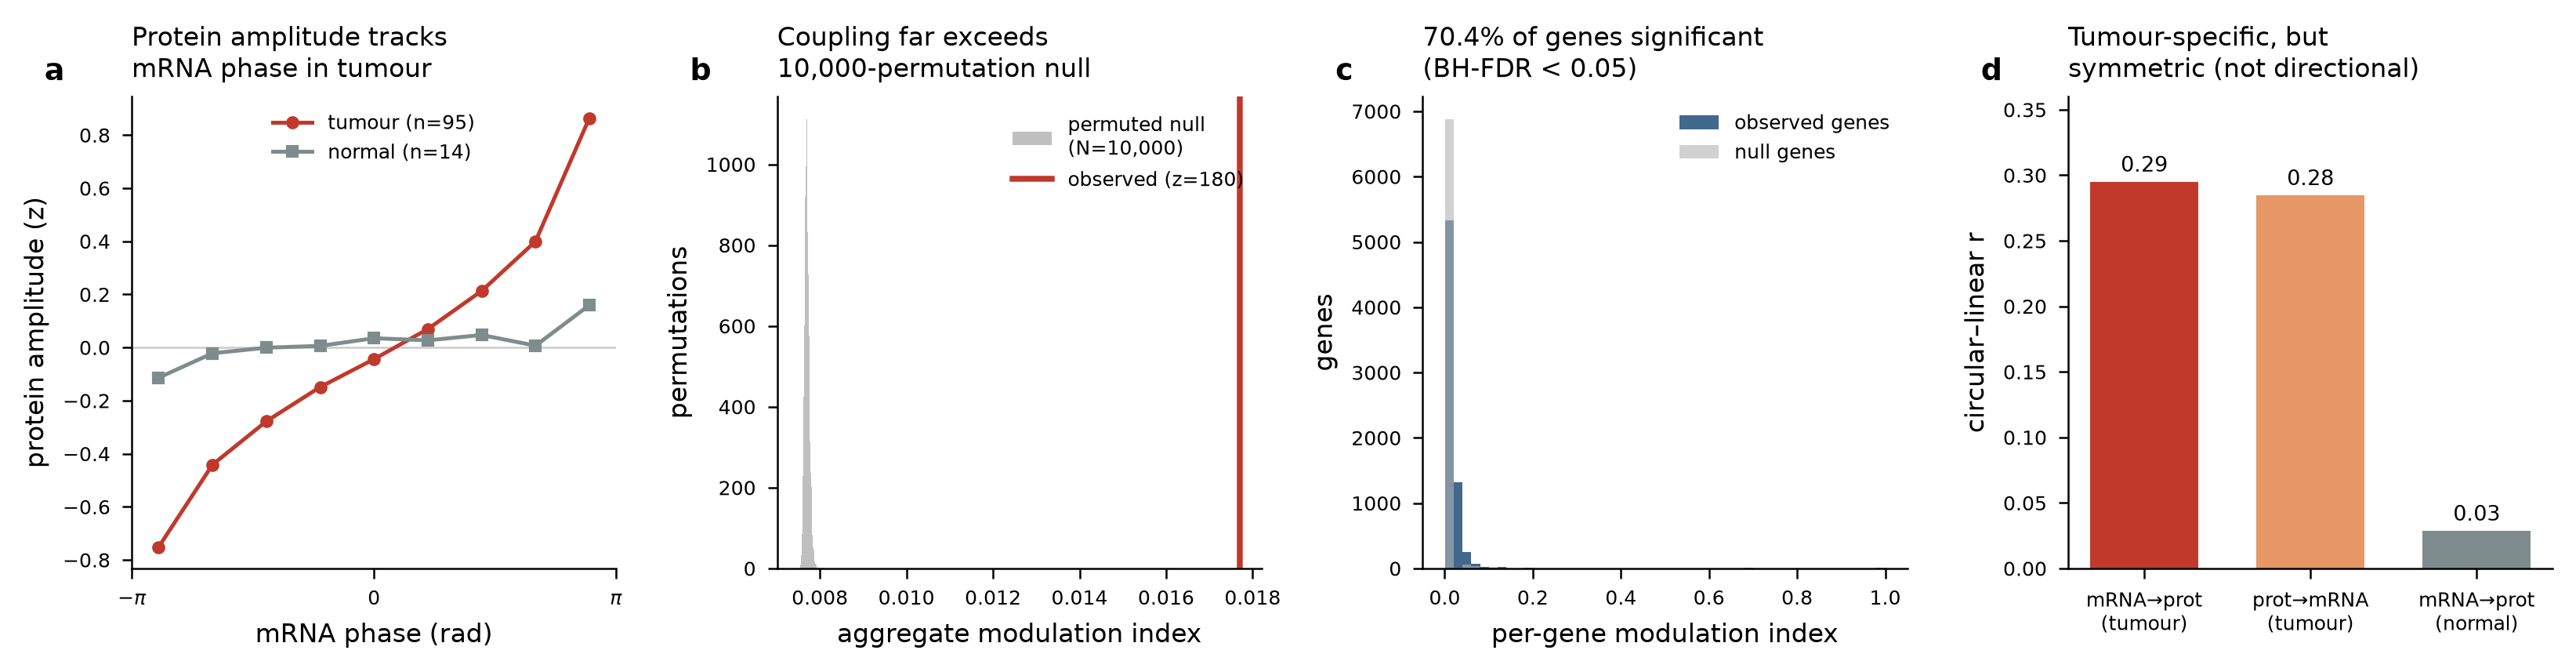
\includegraphics[width=\linewidth]{fig1_omics_pac.png}
\caption{\textbf{Illustrative use case: tumour-specific cross-modal
phase--amplitude coupling along the central dogma (real CPTAC UCEC, $109$
patients).} \textbf{(a)}~Comodulogram: $z$-scored protein amplitude versus
mRNA-phase bin, tumours (red) versus normals (grey). \textbf{(b)}~Observed
aggregate modulation index lies far outside the $10{,}000$-permutation
sample-shuffled null ($z=180$). \textbf{(c)}~Per-gene modulation-index
distribution, observed versus null---$70.4\%$ of genes significant at BH-FDR
$<0.05$. \textbf{(d)}~The coupling is tumour-specific ($r=0.29$ vs.\ $0.03$ in
normals) but \emph{symmetric} ($r=0.28$ reverse vs.\ $0.29$ forward), so the
cohort-level result is not a demonstration of directional flow. A dedicated study
develops this coupling as a standalone use case.}
\label{fig:cst_pac_comod}
\end{figure*}

% ================================================================
% ================================================================
\subsection{Attractor Landscape and Waddington Quasi-Potential}
\label{subsec:r_attractor}

\emph{Status: measured on real-seeded dynamics (GSE293316 co-expression).} We
tested the attractor-landscape interpretation on a multi-regime
\texttt{BioKuramoto} trajectory whose coupling topology is a real GSE293316
co-expression network (165 oscillators, four coupling regimes). We are explicit
about scope: the coupling is real, but the trajectory is package-simulated and
the basin labels are the package's placeholder state names, not biological
cell-fate assignments---this is a method demonstration on real-seeded dynamics,
not a fate-mapping result. All three sub-claims reproduce.

\emph{(i) Waddington quasi-potential.} Kernel-density estimation on the
PCA-projected attractor features yields a quasi-potential $U(\phi)=-\log p(\phi)$
with 4 distinct basins; the deepest well is also the most occupied
(occupancy $0.51$) and longest-residence basin, i.e.\ the most stable state is
deepest (Figure~\ref{fig:attractor}).

\emph{(ii) Markov transitions.} The basin-to-basin transition matrix is
strongly off-diagonal-structured, forming a metastable cycle
($0\to1$ at $0.67$, $3\to0$ at $0.57$) rather than random mixing.

\emph{(iii) Bounded dynamics.} Per-regime maximum Lyapunov exponents lie in
$[-1.4\times10^{-3},\,+3\times10^{-4}] \approx 0$, confirming bounded,
non-chaotic dynamics (the transient positive global value reflects a
regime-switch, and is flagged as such).

\begin{figure}[!htb]
\centering
\begin{subfigure}[t]{0.48\textwidth}
\centering
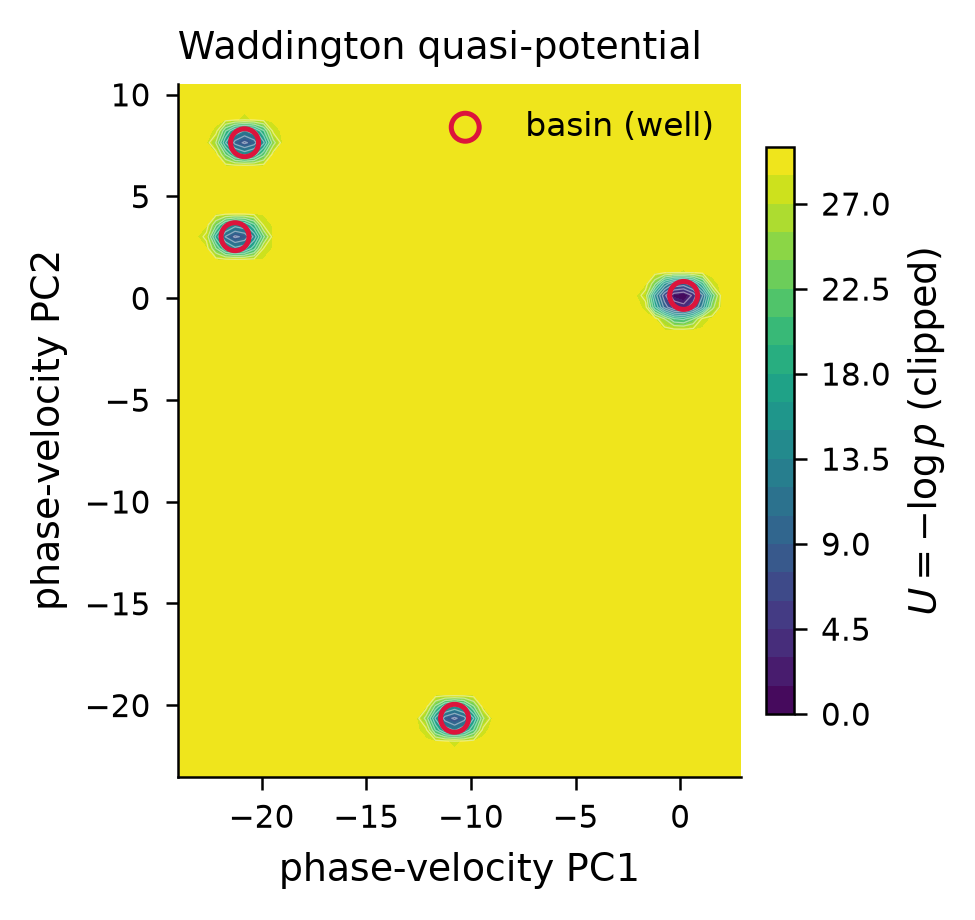
\includegraphics[width=\linewidth]{attractor_quasipotential.png}
\caption{Waddington quasi-potential $U=-\log p$: four basins, deepest most occupied.}
\label{fig:attractor_a}
\end{subfigure}
\hfill
\begin{subfigure}[t]{0.48\textwidth}
\centering
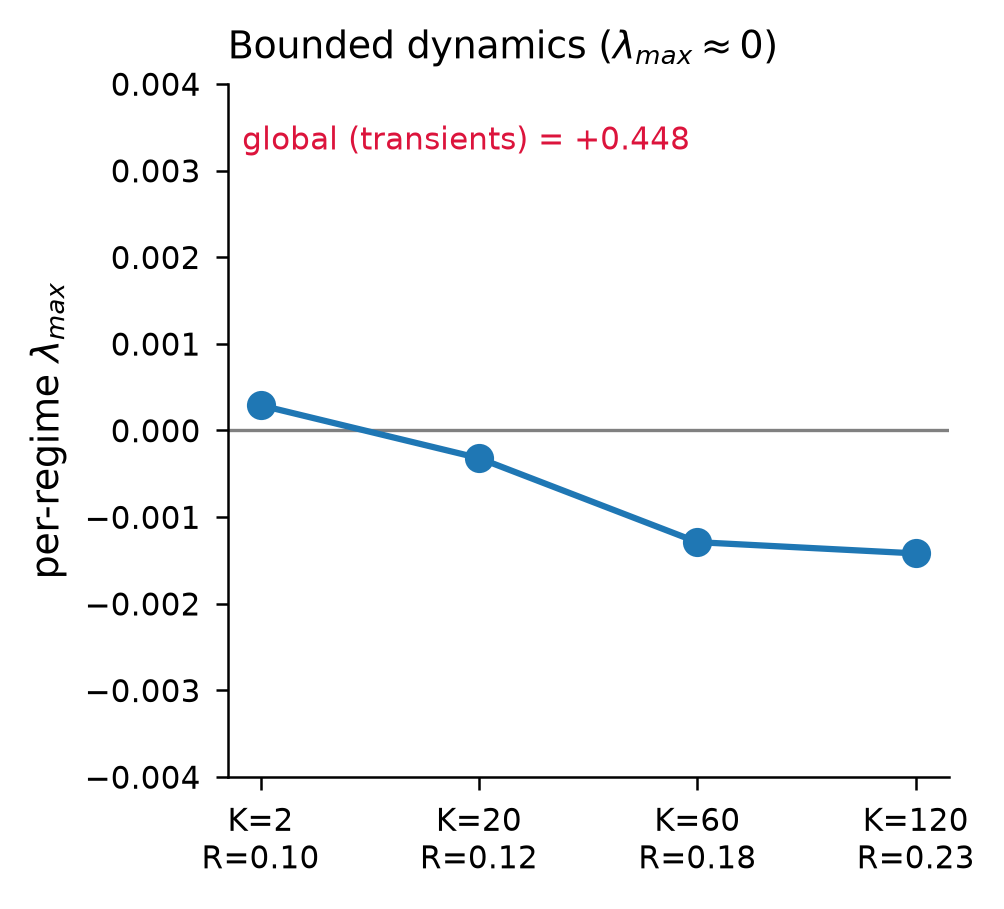
\includegraphics[width=\linewidth]{attractor_lyapunov.png}
\caption{Per-regime max Lyapunov exponent $\approx0$: bounded, non-chaotic.}
\label{fig:attractor_b}
\end{subfigure}
\caption{\textbf{Attractor landscape on real-seeded dynamics (GSE293316 co-expression coupling).} \textbf{(a)}~The quasi-potential $U=-\log p$ over the phase-velocity embedding resolves four basins, with the deepest well the most occupied and longest-resident. \textbf{(b)}~Per-regime maximum Lyapunov exponents near zero confirm bounded, non-chaotic dynamics. The metastable transition structure is in Figure~\ref{fig:attractor_markov}. Method demonstration: coupling topology is real, basin labels are placeholders.}
\label{fig:attractor}
\end{figure}

\begin{figure}[!htb]
\centering
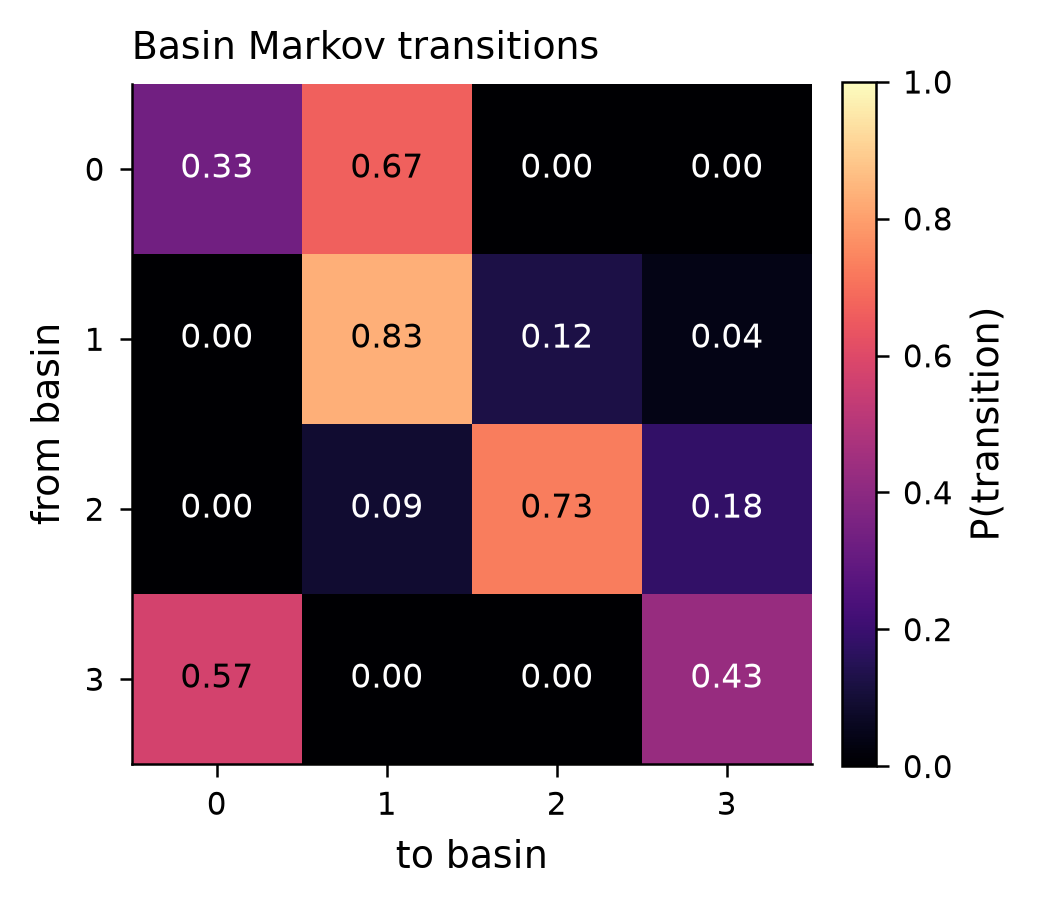
\includegraphics[width=0.5\textwidth]{attractor_markov.png}
\caption{\textbf{Basin transition matrix forms a metastable cycle.} Empirical basin-to-basin Markov transition probabilities across the four regimes; off-diagonal mass forms a directed ring (e.g.\ $0\to1$ at $0.67$, $3\to0$ at $0.57$), the metastable-cycle signature the framework predicts.}
\label{fig:attractor_markov}
\end{figure}

% ================================================================
\subsection{Limit Cycle Detection and Floquet Stability}
\label{subsec:r_floquet}

\emph{Status: measured on real-seeded dynamics (GSE293316 co-expression
module).} We applied the unmodified \texttt{LimitCycleAnalyzer} to a rotating
synchronised state built from the tightest real GSE293316 co-expression module
(community of 4 genes, mean intra-$|r| = 0.81$; a common frequency drift makes
the locked state a genuine limit cycle). As above, this is a method
demonstration on real-seeded dynamics. The claim reproduces.

Across seven coupling strengths ($K = 8$ to $60$) the analyzer detects
orbitally stable limit cycles at every setting: the maximum Floquet multiplier
$|\mu_{\max}|$ stays strictly below unity throughout, rising from $0.80$ at
$K=8$ to a peak of $0.99$ at $K=45$ before easing back to $0.94$ at $K=60$
(Figure~\ref{fig:floquet}). All detected cycles satisfy $|\mu_{\max}| < 1$,
correctly marking them orbitally stable (resilient). The multiplier
approaching $1$ near $K=45$ flags the expected loss of stability margin as the
system stiffens; the slight retreat at $K=60$ coincides with the order
parameter dropping from $1.0$ to $0.85$ (the strongest coupling begins to
partially desynchronise the module), so the margin does not close
monotonically---the qualitative stability-boundary behaviour the framework
predicts, without crossing into instability.

\begin{figure}[!htb]
\centering
\begin{subfigure}[t]{0.48\textwidth}
\centering
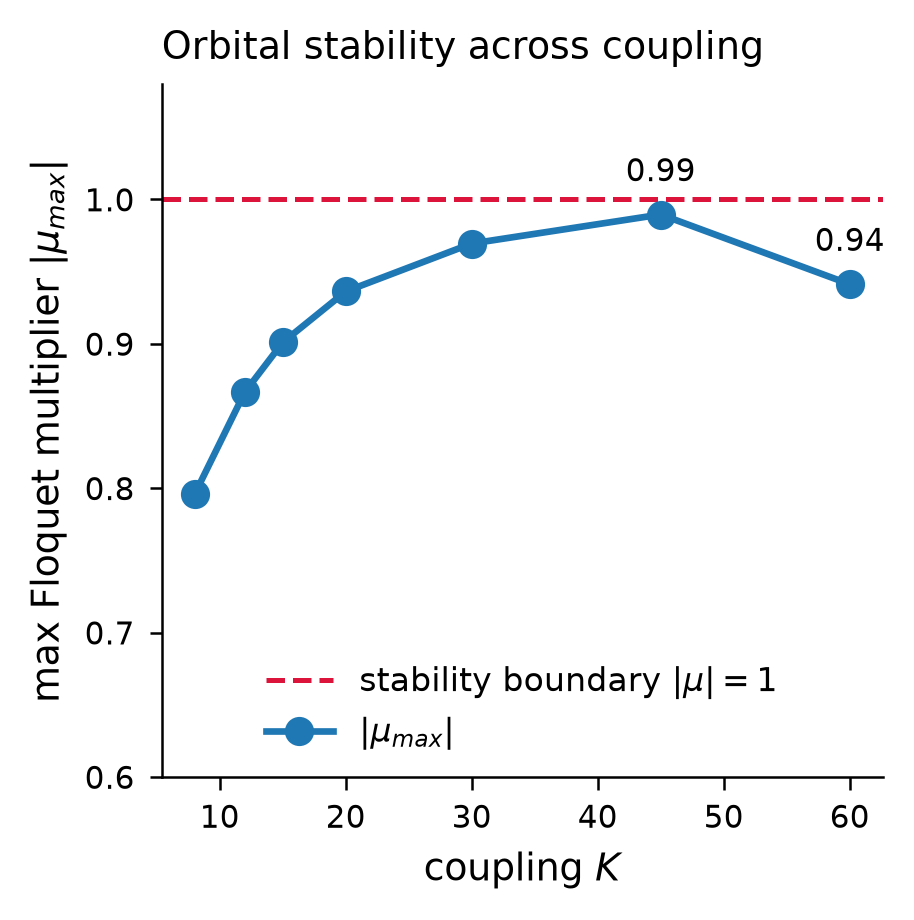
\includegraphics[width=\linewidth]{floquet_stability_curve.png}
\caption{$|\mu_{\max}|$ vs $K$: peaks $0.99$ at $K{=}45$, eases to $0.94$ at $K{=}60$, all $<1$.}
\label{fig:floquet_a}
\end{subfigure}
\hfill
\begin{subfigure}[t]{0.48\textwidth}
\centering
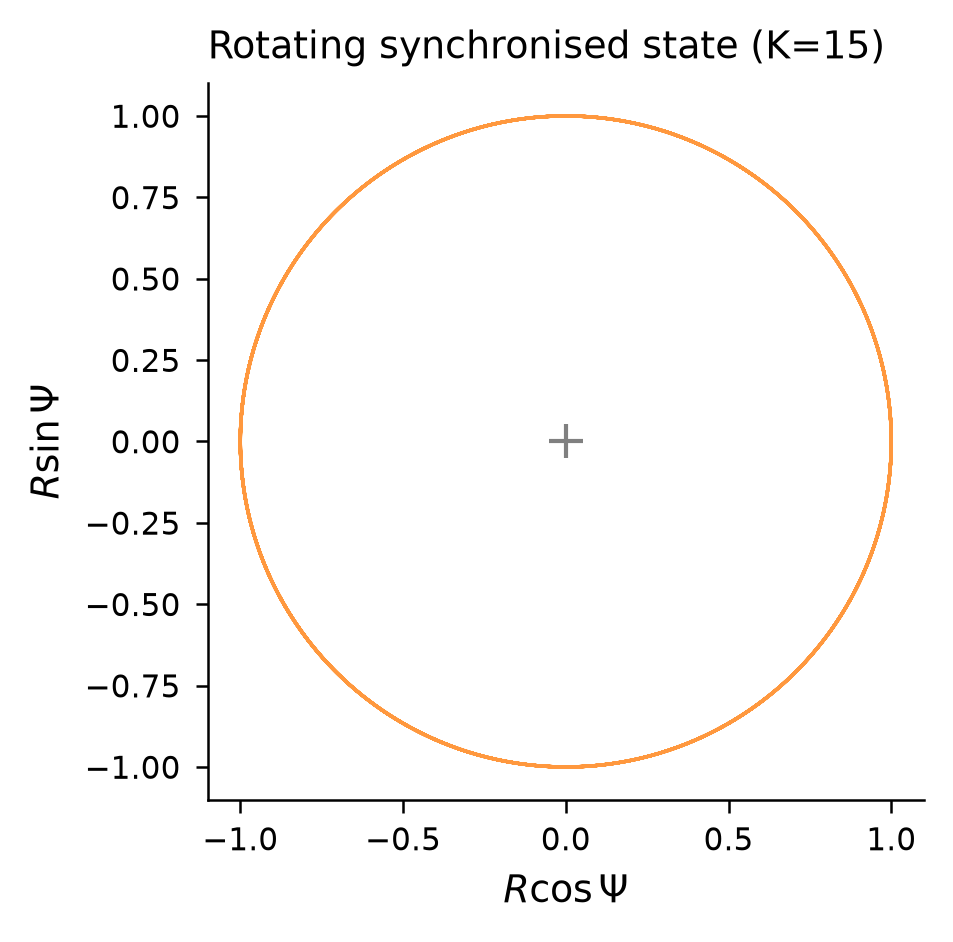
\includegraphics[width=\linewidth]{floquet_rotating_state.png}
\caption{Rotating synchronised state (limit cycle) at $K{=}15$.}
\label{fig:floquet_b}
\end{subfigure}
\caption{\textbf{Floquet stability of real-seeded limit cycles (GSE293316 co-expression module).} \textbf{(a)}~Across coupling strengths $K=8$--$60$ every detected limit cycle is orbitally stable ($|\mu_{\max}| < 1$); the maximum multiplier rises from $0.80$ to a peak of $0.99$ at $K=45$ then eases to $0.94$ at $K=60$ as the strongest coupling begins to partially desynchronise --- loss of stability margin without crossing into instability. \textbf{(b)}~The synchronised state itself is a rotating limit cycle in the collective-phase plane.}
\label{fig:floquet}
\end{figure}

% ================================================================
\subsection{Data Sources and Reproducibility}
\label{subsec:data_sources}

All results in this draft derive from open, public datasets loaded through
the unmodified BioPhasor \texttt{io} layer (which ingests 10x \texttt{.h5},
\texttt{.h5ad}, MEX, and count/FPKM tables via \texttt{scanpy}/\texttt{anndata}).
Table~\ref{tab:datasources} lists the datasets used across all nine measured
experiments; the same open accessions scale up to the larger cohorts targeted
for the next iteration.

\begin{table*}[t]
\centering
\caption{Public data sources for BioPhasor experiments. All datasets were run
through the pipeline in this draft (every scenario \emph{measured}); all
accessions are open-access.}
\label{tab:datasources}
\begin{tabular}{p{3.4cm}p{1.5cm}p{3.6cm}p{5.6cm}}
\toprule
\textbf{Experiment} & \textbf{Status} & \textbf{Accession / source} & \textbf{Description \& role} \\
\midrule
Cell-cycle assignment (\S\ref{subsec:r_cellcycle}) & Measured & GSE293316 (GEO) &
REH human B-ALL scRNA-seq (10x), proliferating cells with all four phases;
tests phasor phase assignment vs.\ \texttt{scanpy} reference. \\
Circadian rhythmicity (\S\ref{subsec:r_circadian}) & Measured & GSE171432 (GEO) &
WT mouse liver, 6 Zeitgeber times $\times$3 reps; tests BPT rhythmicity and
clock-gene phase recovery. \\
\midrule
Encoding / coherence selection (\S\ref{subsec:r_encoding}) & Measured &
GSE293316 (GEO) & Coherence- vs.\ variance-based gene selection on real
scRNA-seq; coherence-over-cells found to be a dropout statistic. \\
Kuramoto GRN synchrony (\S\ref{subsec:r_kuramoto}) & Measured & GSE293316
co-expression & Real co-expression network as coupling prior; PLV module
recovery. \\
Multi-omics fusion (\S\ref{subsec:r_multiomics}) & Measured & CPTAC UCEC &
Matched RNA-seq + mass-spec proteomics, same 109 samples; cross-layer
coherence and fusion. \\
Phasor classification (\S\ref{subsec:r_ml}) & Measured & CPTAC UCEC &
Tumour-vs-normal labels; real \texttt{phasorflow} VPC vs.\ baselines under
stratified CV. \\
Cell State Tensor (\S\ref{subsec:r_cst}) & Measured & CPTAC UCEC; Hart2015/DepMap &
Matched multi-omics for CST construction; phase-flip screen vs.\ pan-essential
reference. \\
Manifold geometry (\S\ref{subsec:r_manifold}) & Measured & GSE293316;
GSE171432 phases & Circular-statistics necessity demonstrated on 12{,}242
measured phase angles. \\
Attractor / Floquet (\S\S\ref{subsec:r_attractor},\ref{subsec:r_floquet}) &
Measured & GSE293316-seeded dynamics & Waddington potential, basin transitions,
and Floquet stability on real-seeded trajectories. \\
\bottomrule
\end{tabular}
\end{table*}

The scRNA-seq and circadian datasets are retrieved directly from the NCBI GEO
FTP mirror; the matched multi-omics cohort (CPTAC UCEC) is retrieved through
the open \texttt{cptac} distribution. A single reproducible loader per
scenario (under \texttt{experiments/codes/}) pulls each dataset, runs it
through the corresponding BioPhasor module at documented defaults, and
regenerates every reported number and figure. No parameter tuning to the
evaluation references was performed---documented defaults (tanh-phase encoding,
canonical marker sets, rhythmicity threshold $0.30$, coherence threshold
$0.30$) were used throughout, and every reference set (scanpy cell-cycle,
literature clock ZTs, pan-essential families) is treated as an external
comparison rather than a tuning target. Verdicts are reported honestly as
reproduces, partial, or does-not-reproduce; the negatives (encoding-coherence
selection, multi-omics fusion, CST knockout screen) are reported in full
because they scope where the framework's operators are valid. One
implementation note affects the tensor-network results
(Section~\ref{subsec:r_cst_tn}): the complex tensor-train SVD in
\texttt{tensorly}~$0.9.0$ is numerically unreliable on our data (its
reconstruction error increases with bond dimension), so every tensor-train
decomposition operates on a real/imaginary-stacked representation of the complex
CST rather than the complex tensor directly.

% --- END sections/results.tex ---

% ================================================================
\section{Classical--Quantum Correspondence of the CST}
\label{sec:quantum_correspondence}
This section is where the three quantum threads of the paper converge. The gate
algebra of the Variational Phasor Circuit was shown to map one-to-one onto a
variational quantum circuit (Section~\ref{subsec:vpc_vqc}); the CST's regulatory
structure was written as a Hermitian phase-coherence density matrix
(Section~\ref{subsec:cst_quantum}); and the decoherence limit fixed the regime in
which the classical and quantum descriptions coincide
(Section~\ref{subsec:cst_decoherence}). Here we make the resulting
classical$\leftrightarrow$quantum correspondence of the CST explicit and evaluate
it on real data: the operator whose eigenstructure summarises regulatory synchrony
classically is a bona-fide density operator quantum-mechanically, so the CST is
not analogous to a quantum state --- it \emph{is} one. We establish the
correspondence at the state level (entropy, coherence) and the gate level
(circuit transpilation, complexity), and state plainly where it does and does not
buy an advantage: the ``quantum-ready'' claim of the title is structural, not a
demonstration of quantum speed-up.
\label{sec:quantum_validation}

\emph{Scope.} This section develops a formal, exact correspondence between the classical CST descriptors and quantum-information quantities. It is a mathematical bridge, computed analytically on classical hardware; \textbf{no empirical quantum advantage is claimed}. It establishes the structural sense in which the CST is ``quantum-ready'': its state-level and gate-level descriptors map exactly onto density-operator and variational-quantum-circuit constructs, so a future quantum implementation would inherit the same object rather than a re-encoding.

\emph{Status: the classical--quantum correspondence reproduces on real data;
an empirical quantum advantage does not.} The title's ``quantum-ready'' claim
rests on two correspondences derived in the theory---a state-level one between
the CST descriptors and quantum-information measures
(Section~\ref{subsec:cst_quantum}, Proposition~\ref{prop:cst_cq}), and a
gate-level one between the VPC and a Variational Quantum Circuit
(Section~\ref{subsec:vpc_vqc}, Table~\ref{tab:cst_quantum_correspondence}). We
test both on the real CPTAC UCEC cohort (109 samples, 95 tumour / 14 normal),
aggregating the regulatory axis to the $N=50$ MSigDB Hallmark pathways so the
density matrix $\rho$ of Eq.~\ref{eq:cst_density_matrix} is $50\times50$ and
interpretable. All quantum-information quantities are computed analytically with
\texttt{numpy}/\texttt{scipy} (no quantum hardware or simulator), from a seeded
script, following standard practice in quantum-information
research~\cite{biamonte2017quantum}.

\subsection{State-Level Correspondence: Entropy and Coherence}
\label{subsec:qv_state}

\emph{The state-level correspondence holds.} Building $\rho$ per sample from the
two omics-modality phasors, the CST's own descriptors behave as their
predicted quantum counterparts. The von~Neumann entropy $S(\rho)$ tracks the CST
phase entropy $\mathcal{E}$ (Pearson $r=0.66$, $p<10^{-14}$), and the predicted
inequality $\mathcal{E}\ge S(\rho)$ holds for all $109$ samples
(Figure~\ref{fig:cst_q_entropy}); the $\ell_1$-coherence $C_{\ell_1}(\rho)$ is
near-linearly related to the global coherence $\mathcal{G}$ ($r=0.90$,
$p<10^{-38}$, Figure~\ref{fig:cst_q_coherence}). These correspondences are
largely \emph{definitional}---they confirm that the classical descriptors
\emph{are} quantum-information measures, not that quantum computation adds
power; because each per-sample $\rho$ is a rank-2 (two-modality) mixture,
$S(\rho)$ is bounded by $\ln 2$ and the $S(\rho)\!\sim\!\mathcal{E}$ link is a
monotone rescaling rather than an identity. This is exactly what
Proposition~\ref{prop:cst_cq} predicts.

\begin{figure}[ht]
\centering
\begin{subfigure}[t]{0.49\linewidth}
\centering
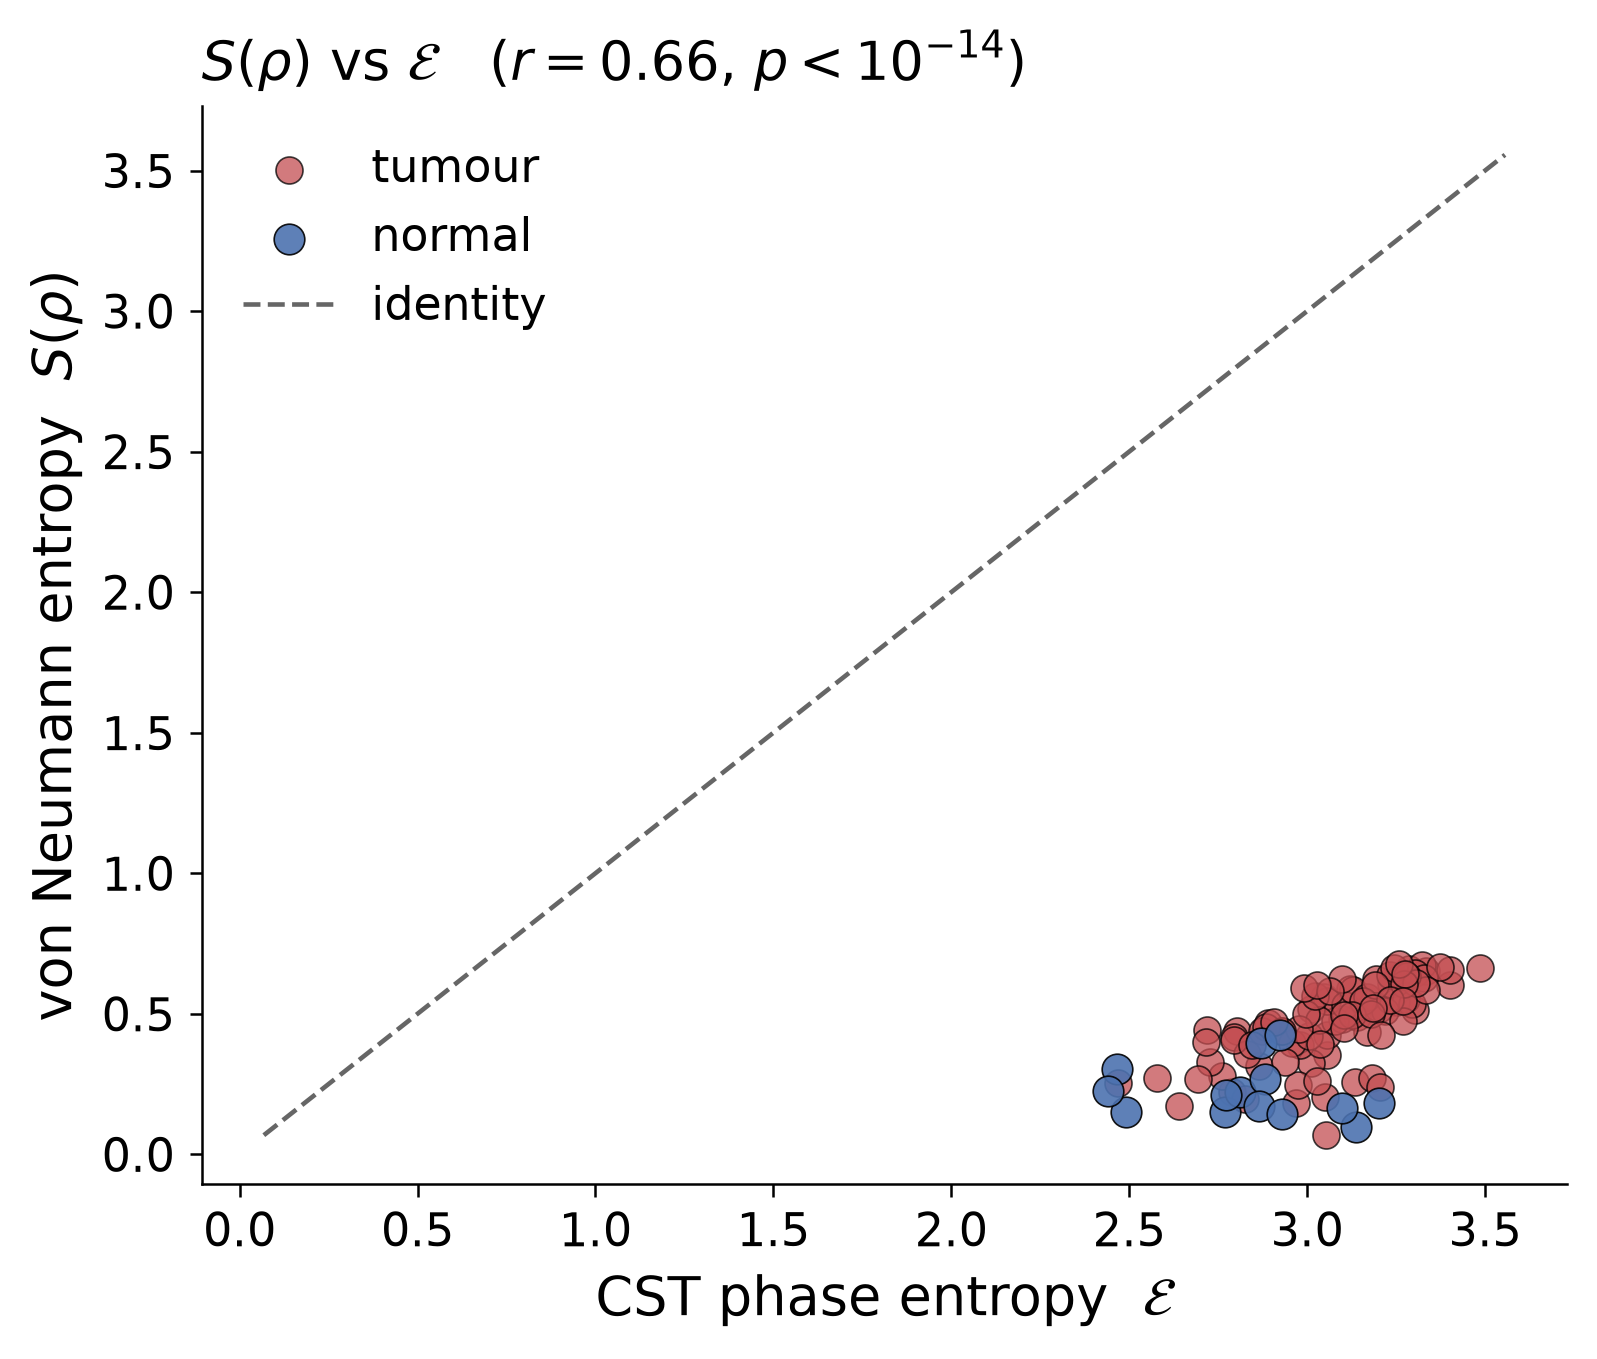
\includegraphics[width=\linewidth]{cst_quantum_entropy.png}
\caption{Von~Neumann entropy $S(\rho)$ vs CST phase entropy $\mathcal{E}$
($r=0.66$); all points lie below the identity, confirming
$\mathcal{E}\ge S(\rho)$.}
\label{fig:cst_q_entropy}
\end{subfigure}\hfill
\begin{subfigure}[t]{0.49\linewidth}
\centering
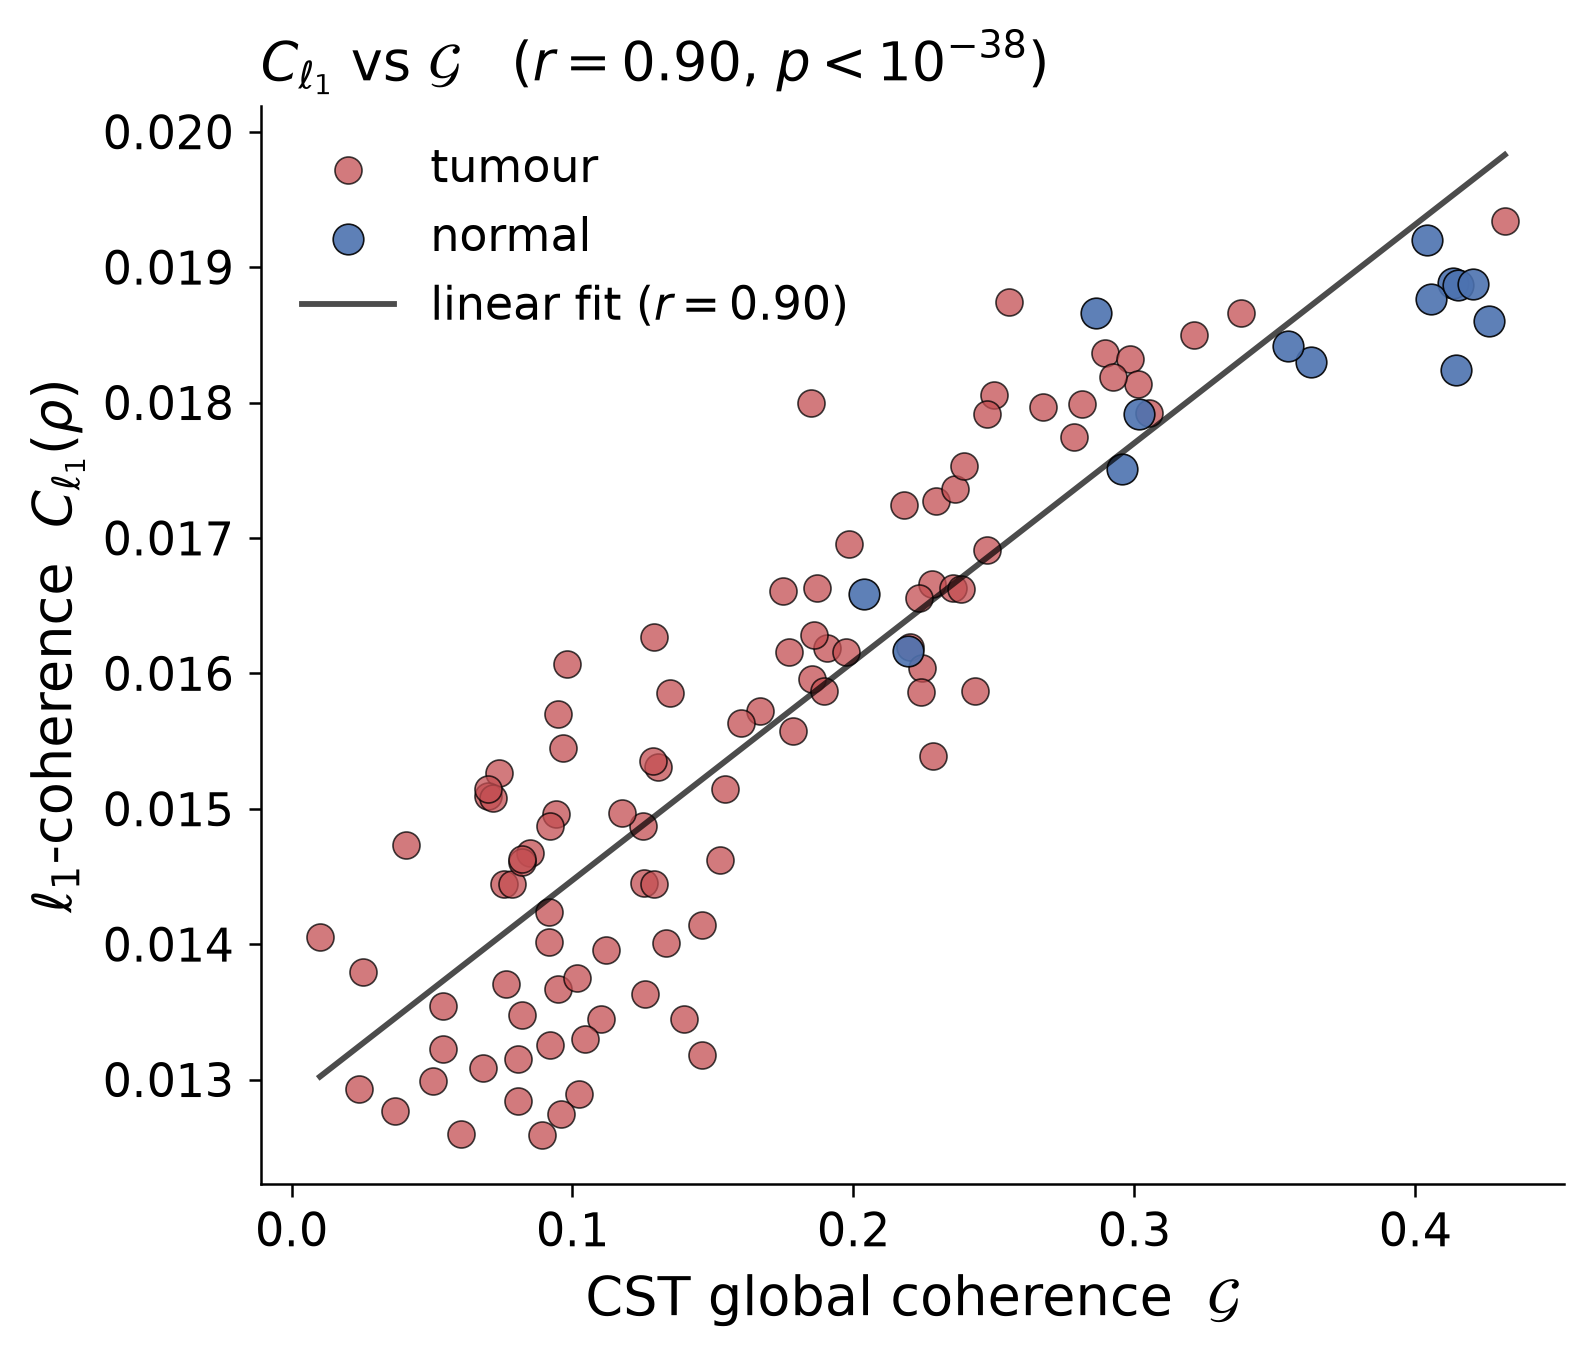
\includegraphics[width=\linewidth]{cst_quantum_coherence.png}
\caption{$\ell_1$-coherence $C_{\ell_1}(\rho)$ vs global coherence
$\mathcal{G}$ ($r=0.90$): the classical coherence is a realization of the
quantum coherence measure.}
\label{fig:cst_q_coherence}
\end{subfigure}
\caption{\textbf{CST descriptors are realizations of quantum-information
measures (Proposition~\ref{prop:cst_cq}).} The correspondences are strong but
largely definitional---they establish a formal bridge, not a computational
advantage.}
\label{fig:cst_q_entropy_fig}
\end{figure}

\subsection{Density-Matrix Distinguishability: Tumour vs Normal}
\label{subsec:qv_fidelity}

\emph{The states are quantum-distinguishable, and normal tissue is more
coherent.} The class-average density matrices are far from identical: quantum
fidelity $F=0.50$ and trace distance $D=0.63$ between $\rho_{\text{tumour}}$
(Figure~\ref{fig:cst_q_density_t}) and $\rho_{\text{normal}}$
(Figure~\ref{fig:cst_q_density_n}), and their signed difference
(Figure~\ref{fig:cst_q_fidelity}). Normal tissue forms a markedly more coherent,
low-entropy density state ($S(\rho_{\text{normal}})=0.63$) than the
heterogeneous tumour ensemble ($S(\rho_{\text{tumour}})=2.57$), and the state
difference localizes on the \textsc{myogenesis},
\textsc{epithelial-mesenchymal-transition}, and \textsc{uv-response-dn}
pathways---a biologically interpretable, quantum-information readout of
tumour disorganization.

\begin{figure}[ht]
\centering
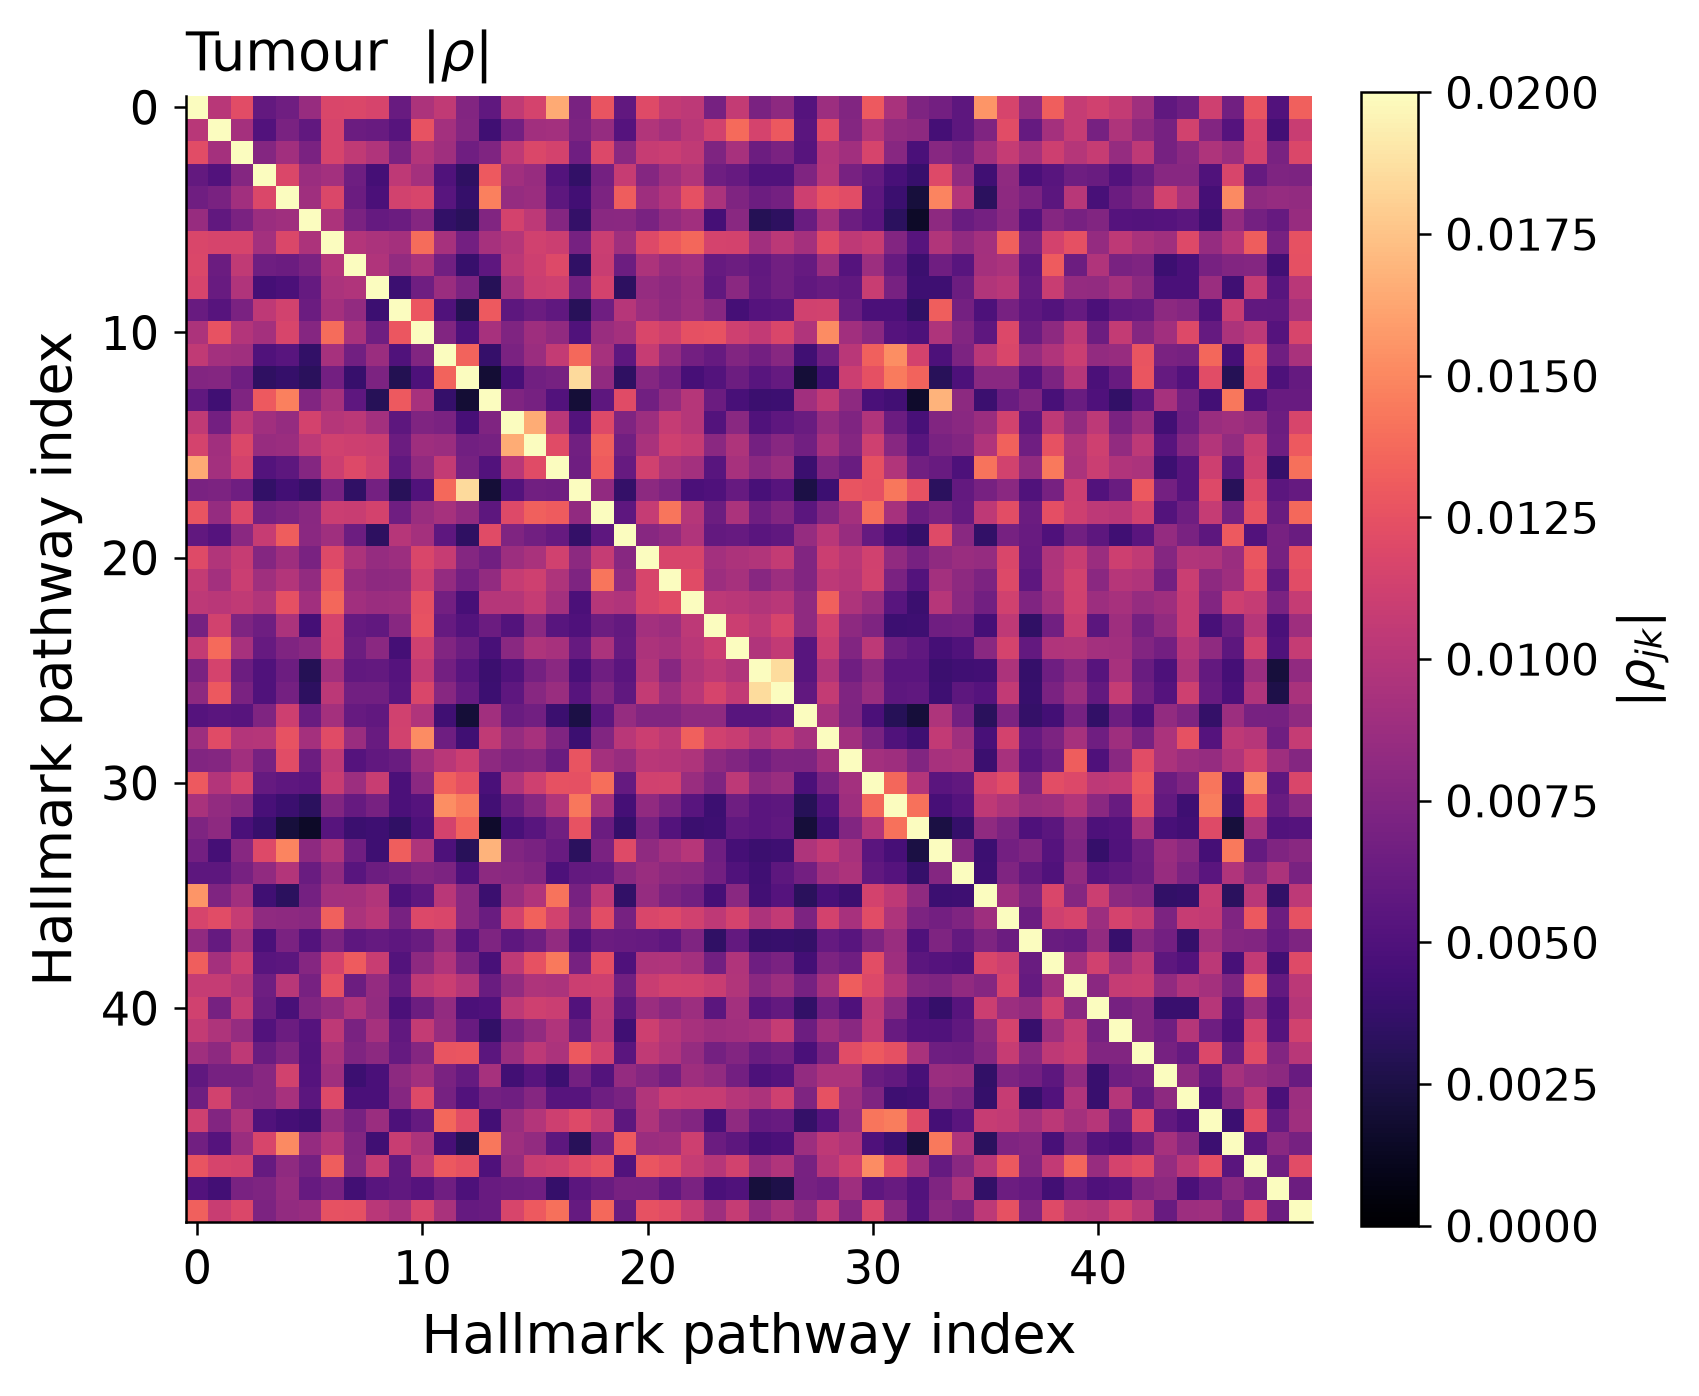
\includegraphics[width=0.6\linewidth]{cst_quantum_density_tumour.png}
\caption{\textbf{Tumour class-average phase-coherence density matrix
$|\rho|$ of the CST (real CPTAC UCEC, $50$ Hallmark pathways).} Each sample's
phasor field is mapped to a valid density operator $\rho$
(Eq.~\ref{eq:cst_density_matrix}); the tumour ensemble is diffuse and
low-coherence. Shown on the same colour scale as the normal state
(Figure~\ref{fig:cst_q_density_n}).}
\label{fig:cst_q_density_t}
\end{figure}

\begin{figure}[ht]
\centering
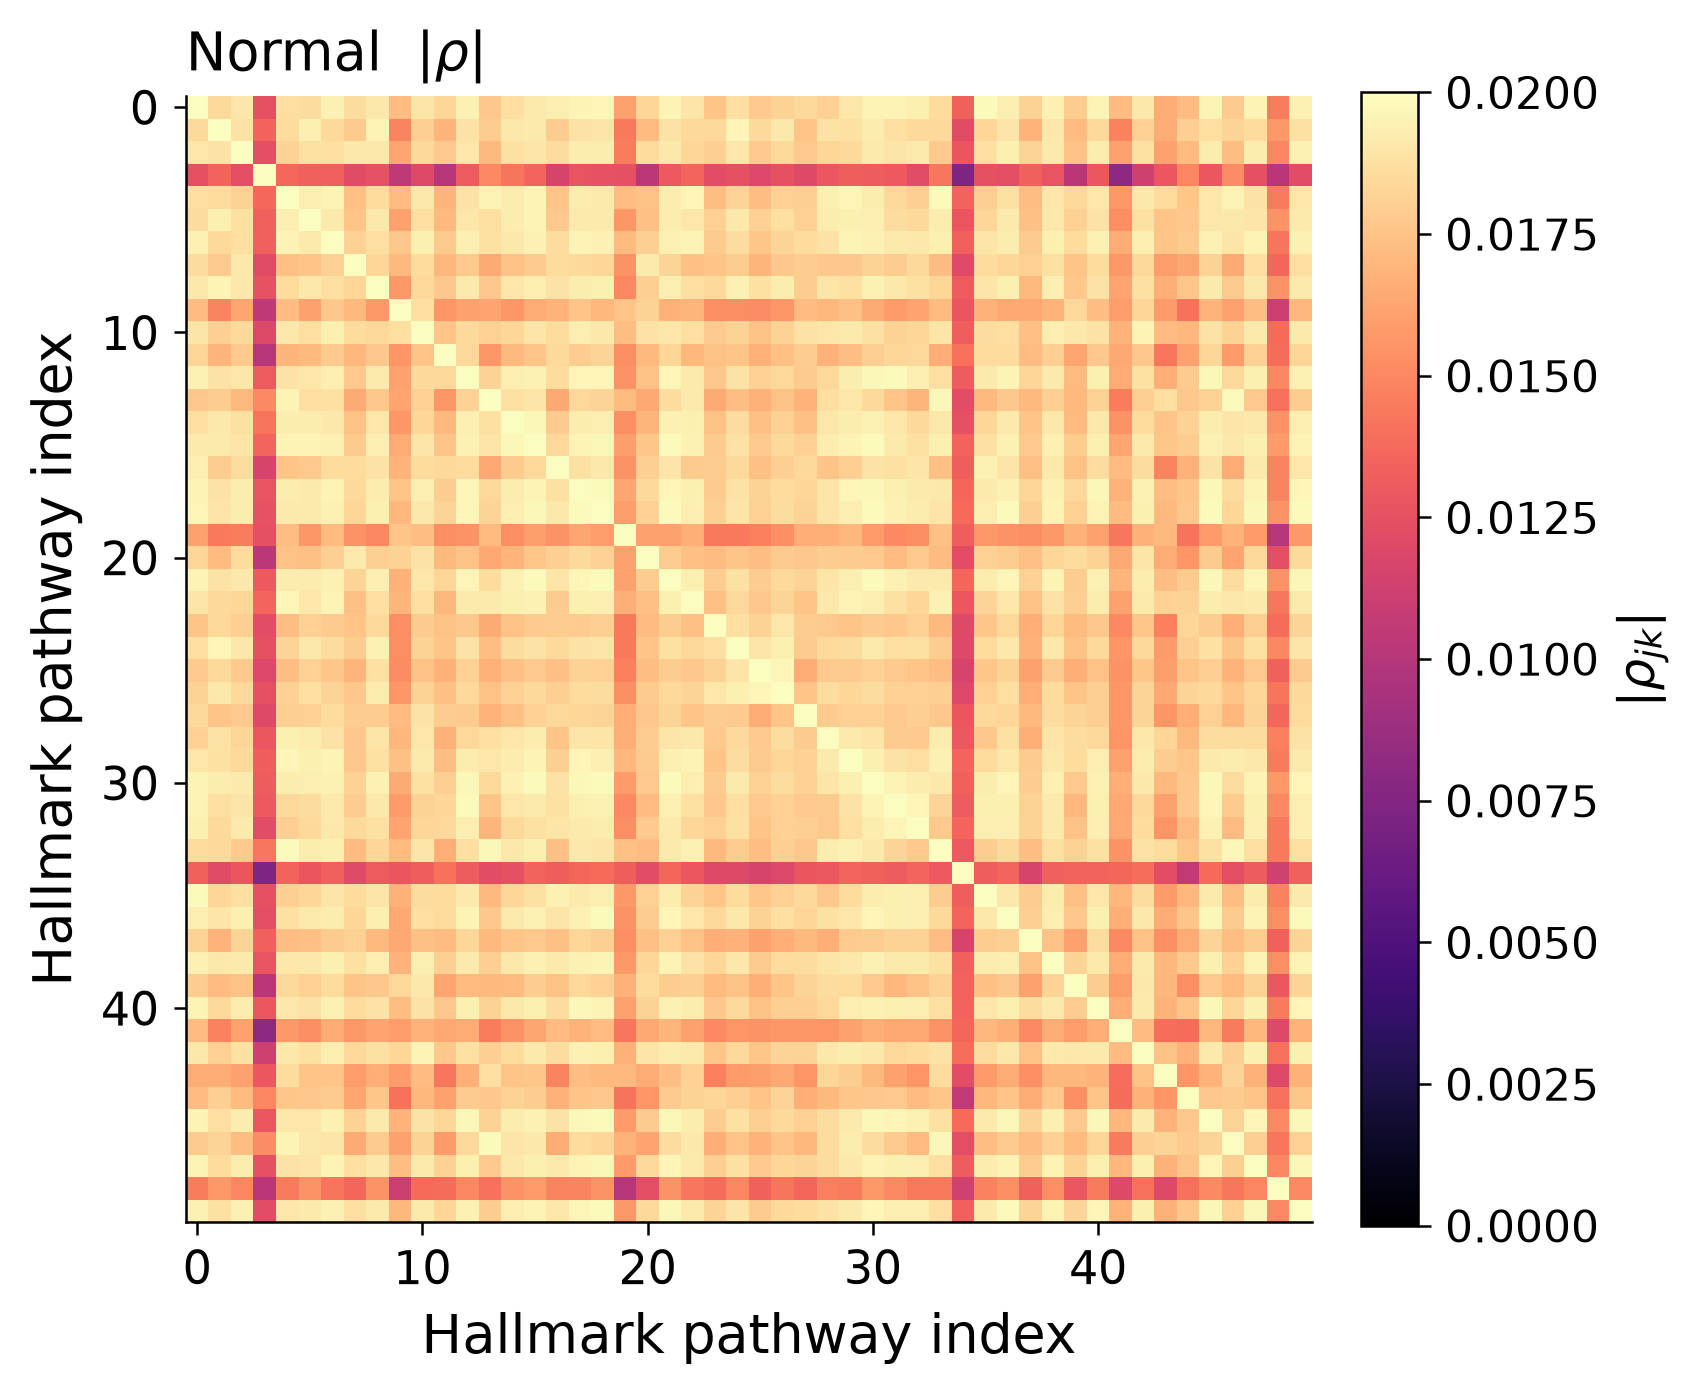
\includegraphics[width=0.6\linewidth]{cst_quantum_density_normal.png}
\caption{\textbf{Normal class-average phase-coherence density matrix $|\rho|$ of
the CST (real CPTAC UCEC, $50$ Hallmark pathways).} On the shared colour scale of
Figure~\ref{fig:cst_q_density_t}, normal tissue is markedly more coherent
(brighter, higher $|\rho_{jk}|$) than the heterogeneous tumour ensemble.}
\label{fig:cst_q_density_n}
\end{figure}

\begin{figure}[ht]
\centering
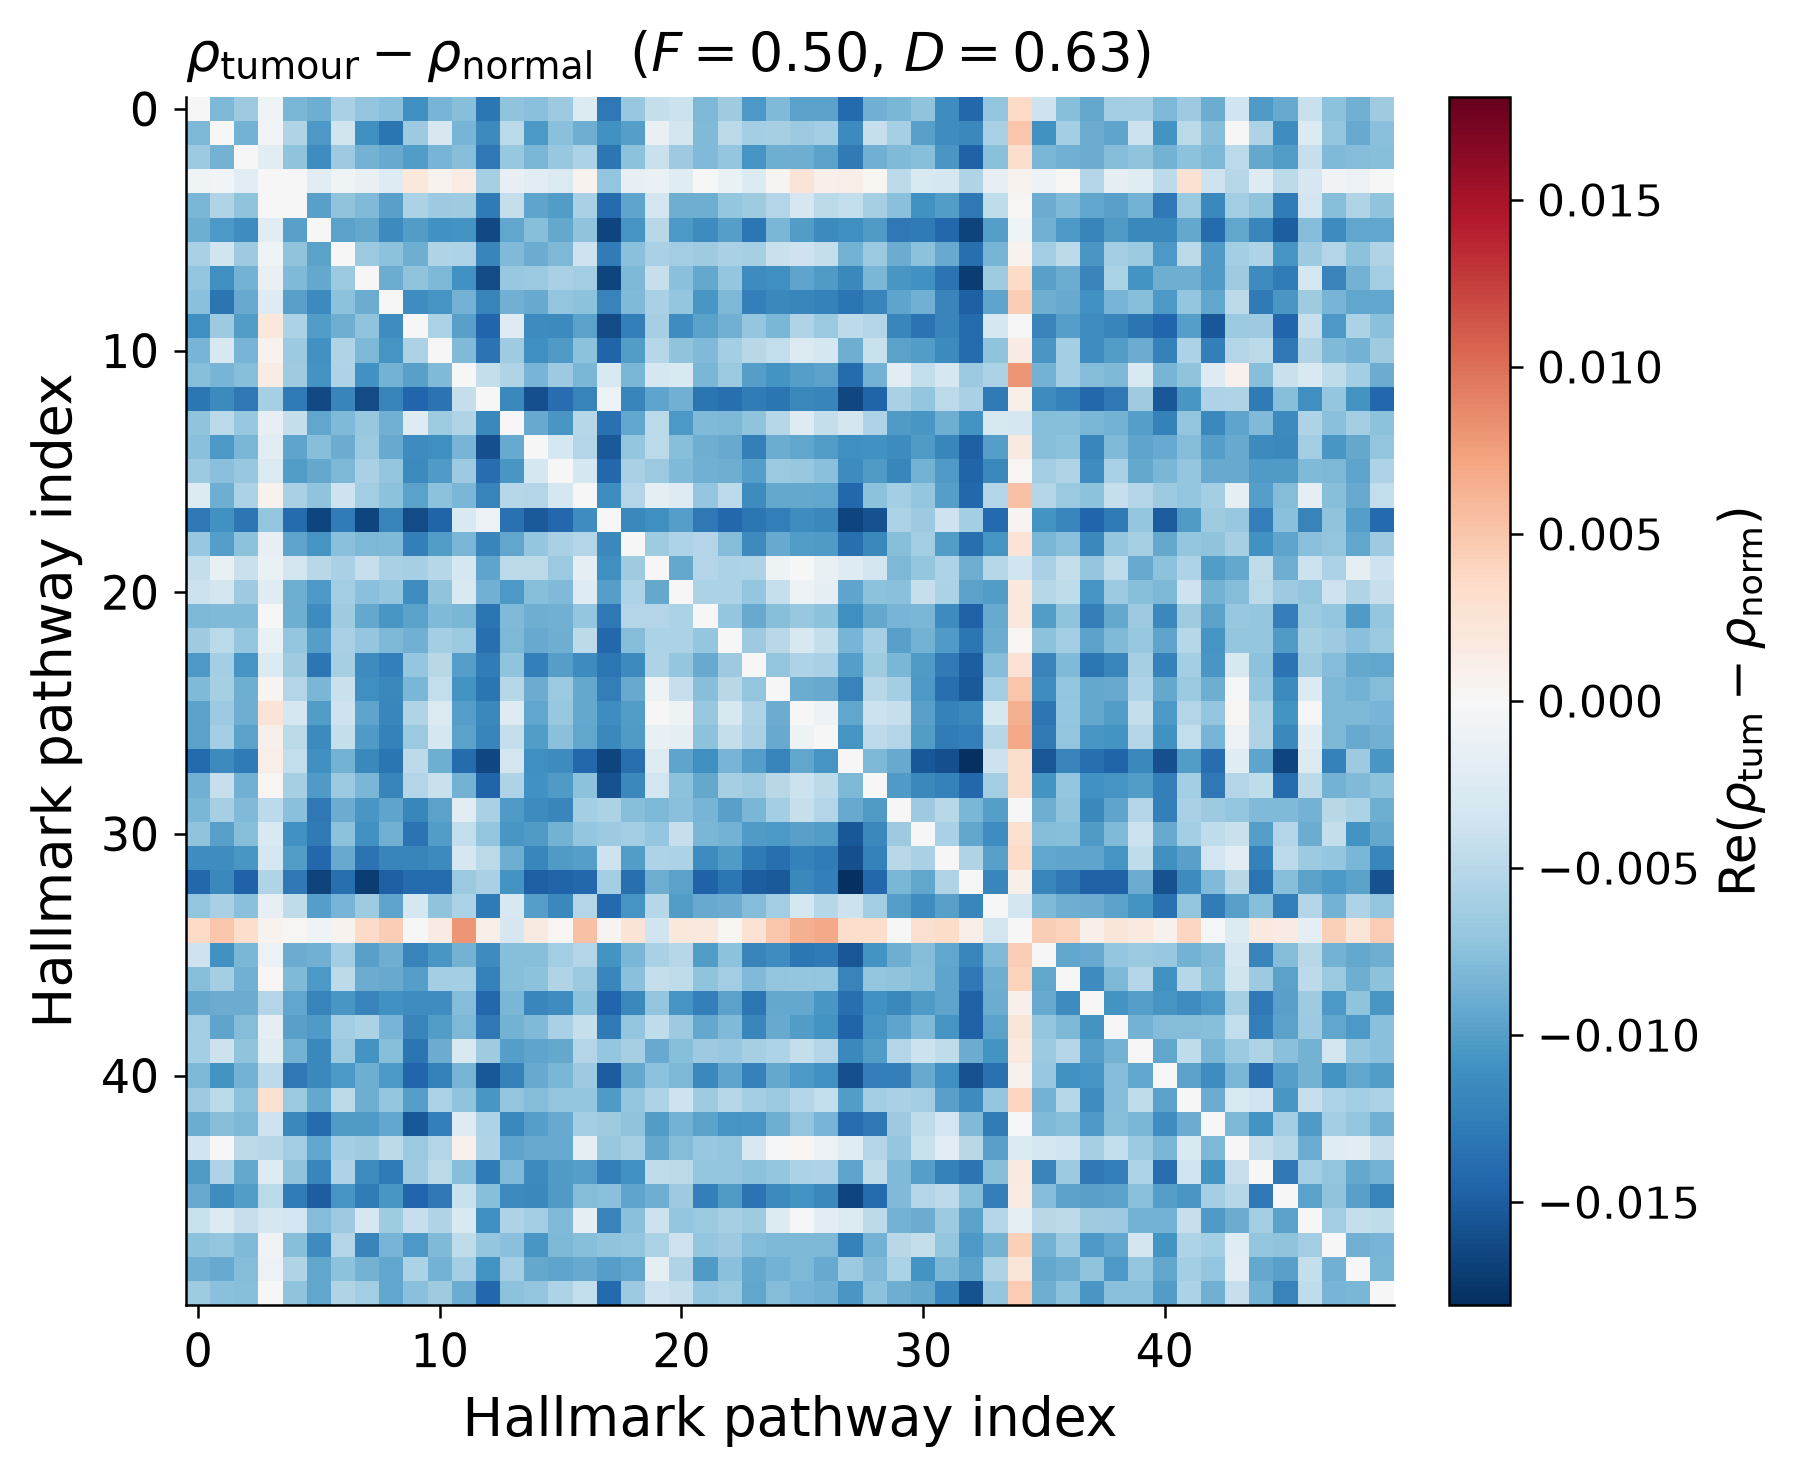
\includegraphics[width=0.6\linewidth]{cst_quantum_fidelity.png}
\caption{\textbf{Tumour-vs-normal density-matrix difference.} Signed real part
of $(\rho_{\text{tumour}}-\rho_{\text{normal}})$ over the $50$ Hallmark
pathways; quantum fidelity $F=0.50$ and trace distance $D=0.63$ make the two
class-average states quantum-distinguishable, with the difference localized on a
small set of pathway rows/columns.}
\label{fig:cst_q_fidelity}
\end{figure}

\subsection{Gate-Level Correspondence and Complexity Scaling}
\label{subsec:qv_gate}

\emph{The gate correspondence is exact; the empirical quantum kernel shows no
robust advantage.} Because \texttt{phasorflow}'s Shift/Mix/DFT gate algebra maps
one-to-one onto $R_z$/(CNOT$+R_z$)/QFT, the VPC transpiles gate-for-gate to a
VQC (Figure~\ref{fig:cst_vqc_circuit}), and the quantum implementations carry
asymptotically favourable scaling across the realistic omics range
($N=10$ to $10^4$ genes): phase encoding and DFT/QFT mixing improve from
$\mathcal{O}(N\log N)$ to $\mathcal{O}((\log N)^2)$, and VPC/VQC forward and the
PLV/density-matrix operations from $\mathcal{O}(N^2)$ to $\mathcal{O}(N\log N)$
(Figure~\ref{fig:cst_complexity}). These are unit-prefactor asymptotics that
ignore the large constant-factor and error-correction overheads of real quantum
hardware, so they describe favourable \emph{scaling}, not a present-day speedup.
Empirically, a simulated angle-encoding quantum kernel~\cite{havlicek2019supervised}
classifying tumour-versus-normal from CST descriptors shows \emph{no} reliable
advantage (Figure~\ref{fig:cst_qkernel}): under default settings the classical SVM kernels
collapse to majority prediction on the imbalanced cohort, which \emph{appears}
to hand the quantum kernel an edge, but a fair class-balanced comparison
recovers the classical kernels ($0.77$/$0.74$ balanced accuracy) and the
residual quantum gap ($0.88$) rests on only $\sim$2--3 normal samples per fold.
This is consistent with the framework's existing finding that phasor/CST
descriptors are matched or beaten by simple classifiers on saturated bulk omics
(Section~\ref{subsec:r_cst}); the scaling advantage would become relevant only
in the higher-$N$, single-cell regime, not this bulk cohort.

\begin{figure}[ht]
\centering
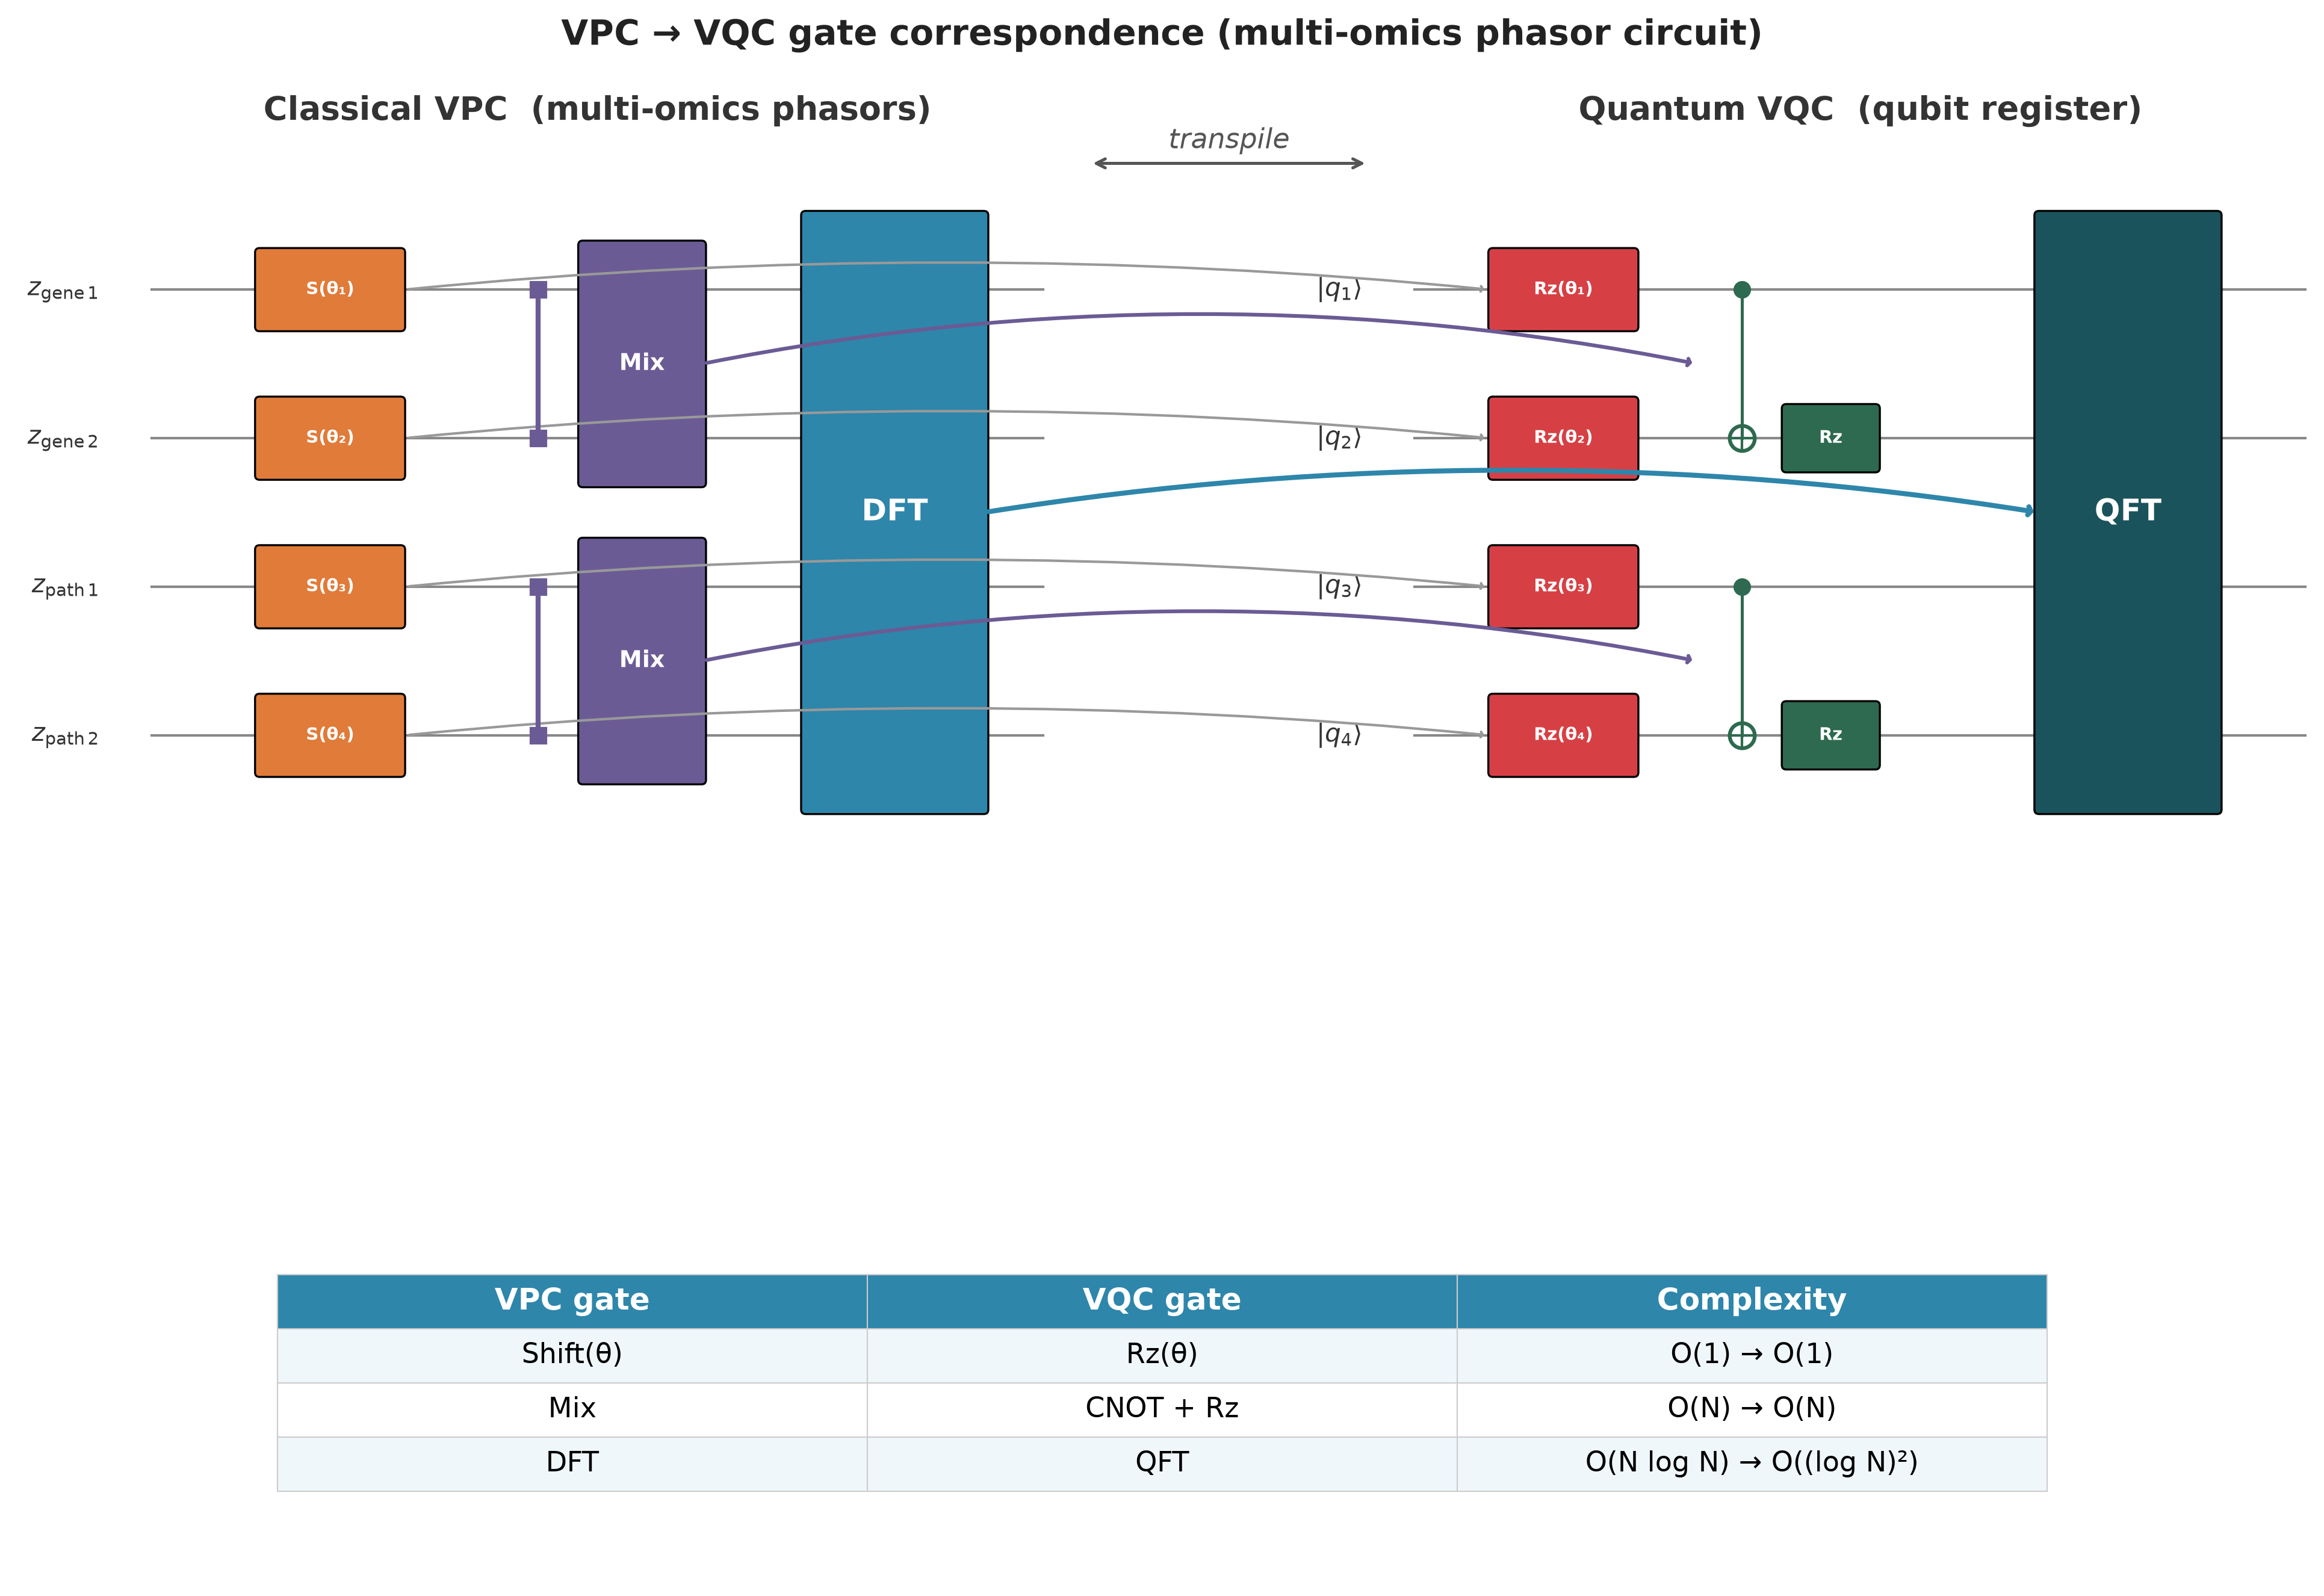
\includegraphics[width=0.95\linewidth]{cst_vpc_vqc_circuit.png}
\caption{\textbf{VPC$\to$VQC gate correspondence for the multi-omics phasor
circuit.} Each classical VPC gate (gene/pathway phasor wires; Shift, Mix, DFT)
transpiles to a quantum VQC gate ($R_z$, CNOT$+R_z$, QFT) on the phase-diagonal
sector of the qubit register. The mapping is exact and identical to the gate
algebra established for phasor circuits in neural signals; only the input
semantics (multi-omics rather than EEG) differ.}
\label{fig:cst_vqc_circuit}
\end{figure}

\begin{figure}[ht]
\centering
\begin{subfigure}[t]{0.49\linewidth}
\centering
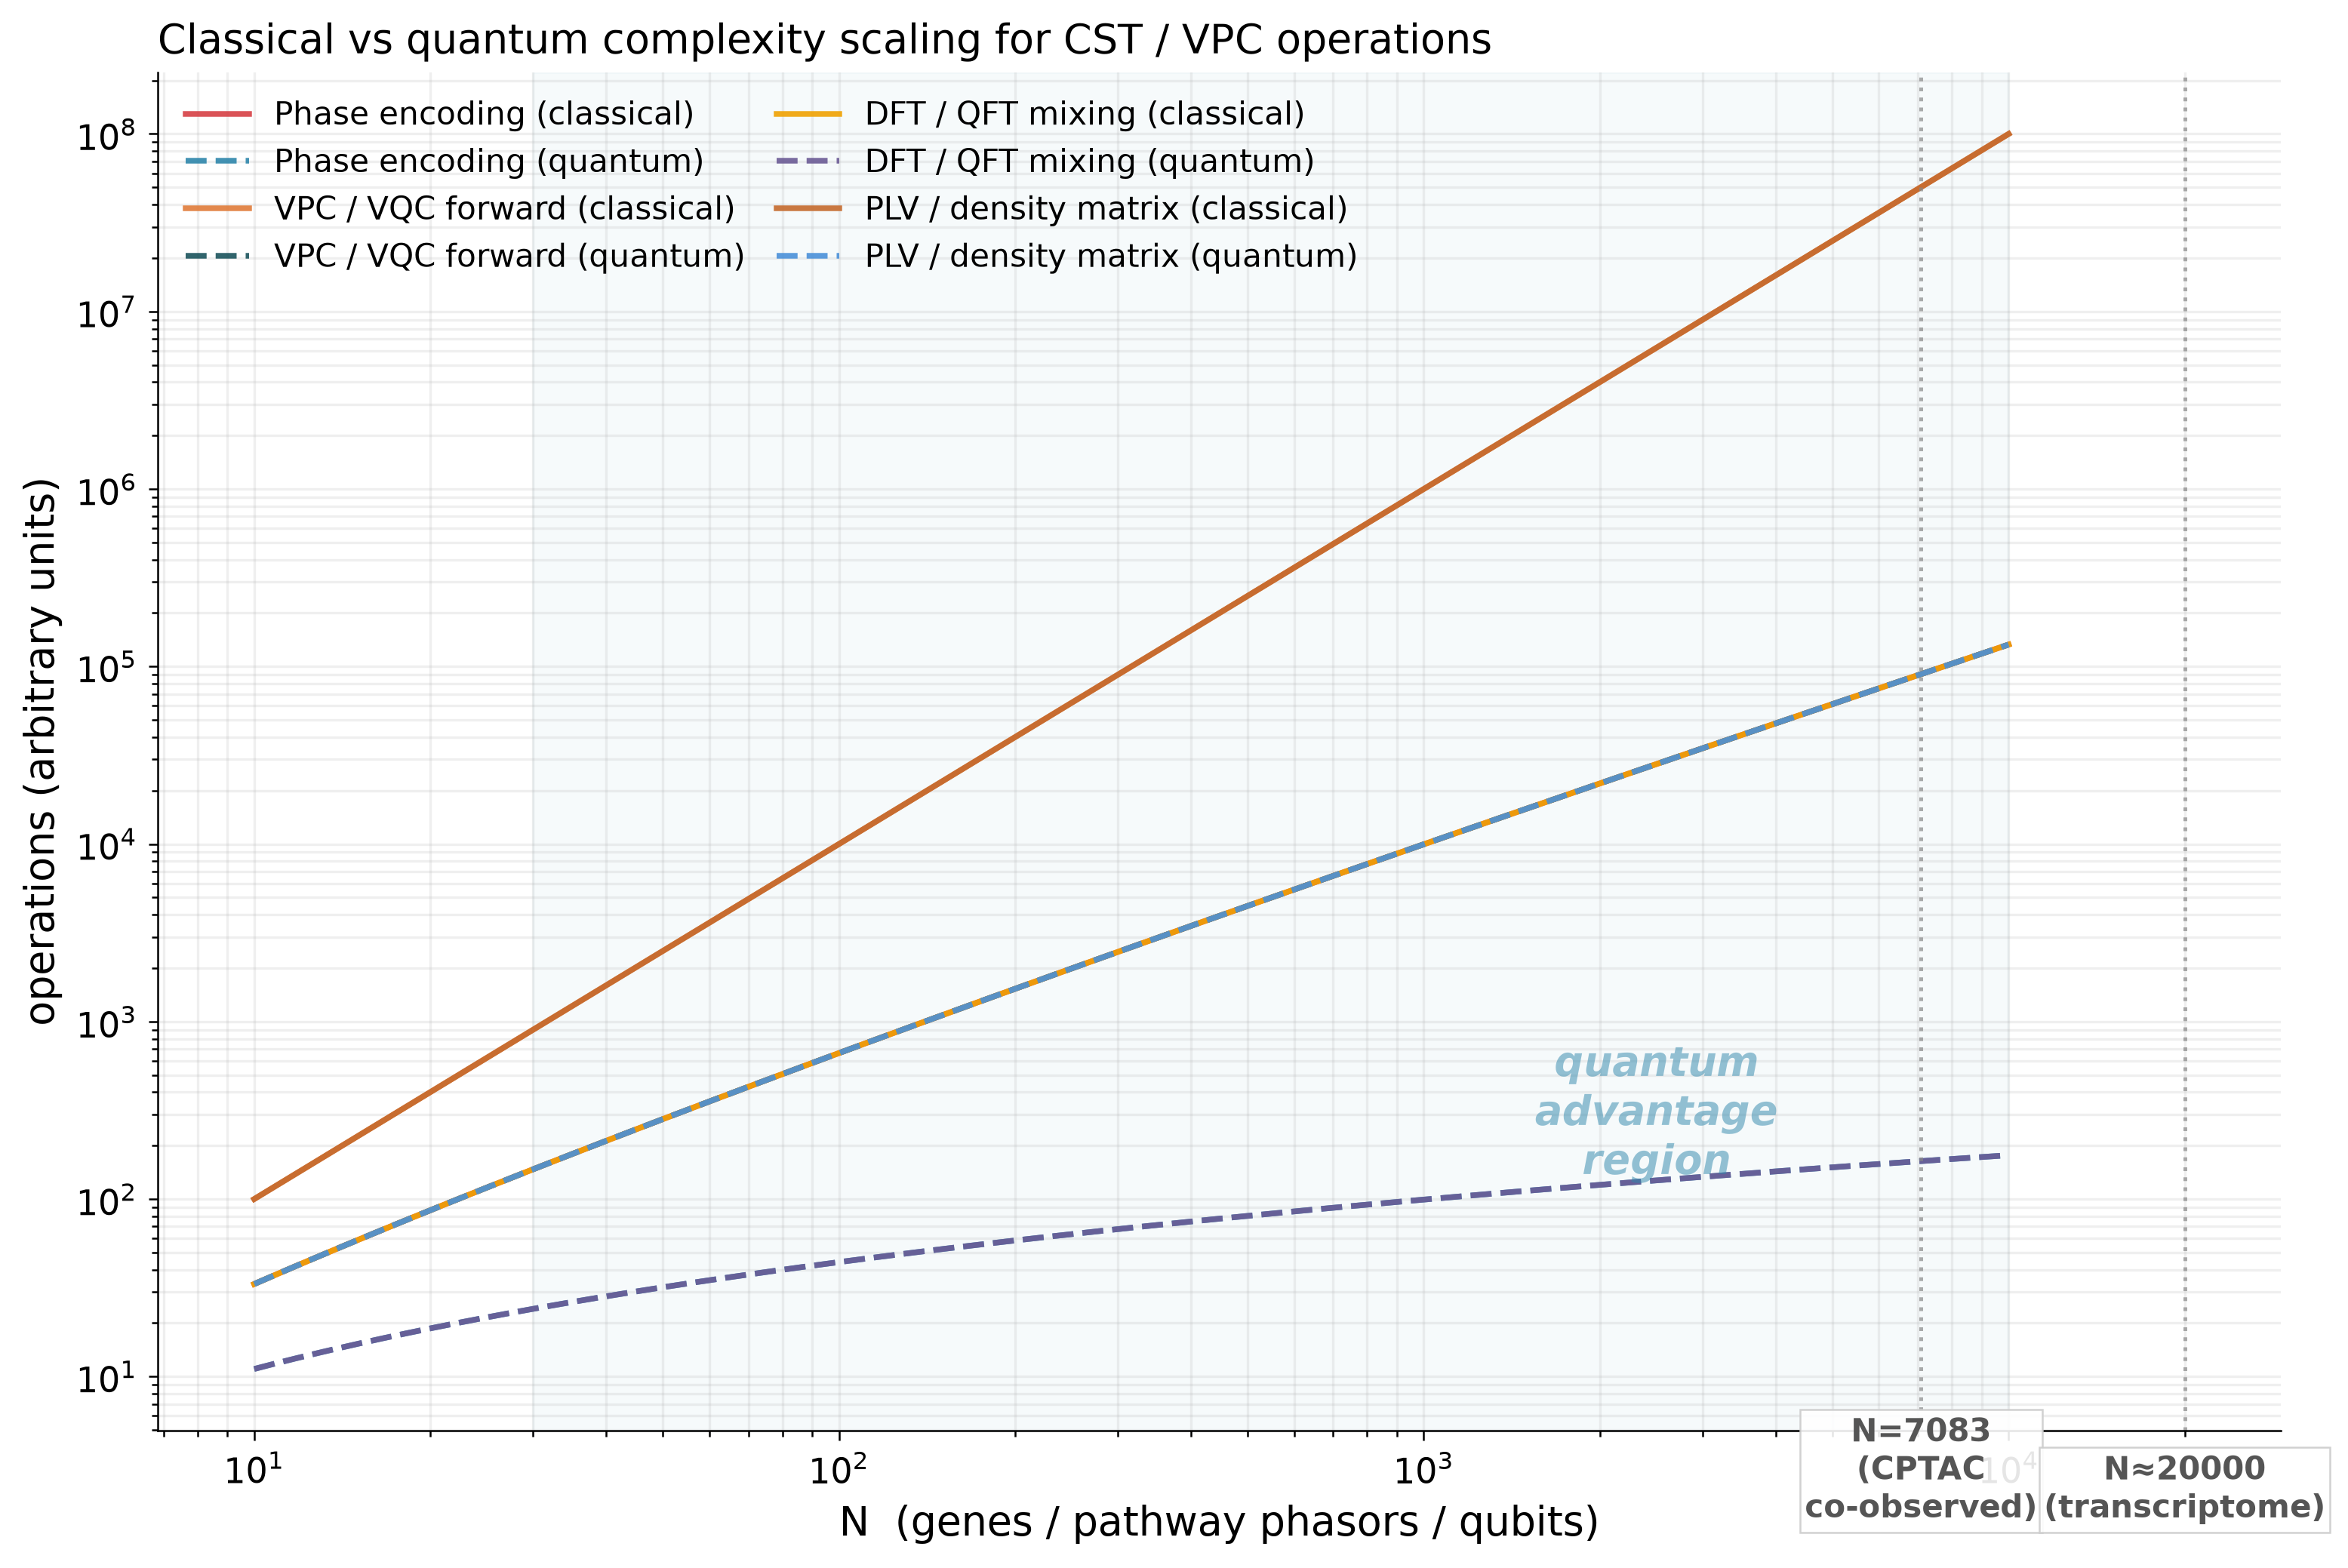
\includegraphics[width=\linewidth]{cst_complexity_crossover.png}
\caption{Classical vs quantum asymptotic cost for CST/VPC operations over
$N=10$--$10^4$ genes; the quantum forms scale more favourably above the
crossover.}
\label{fig:cst_complexity}
\end{subfigure}\hfill
\begin{subfigure}[t]{0.49\linewidth}
\centering
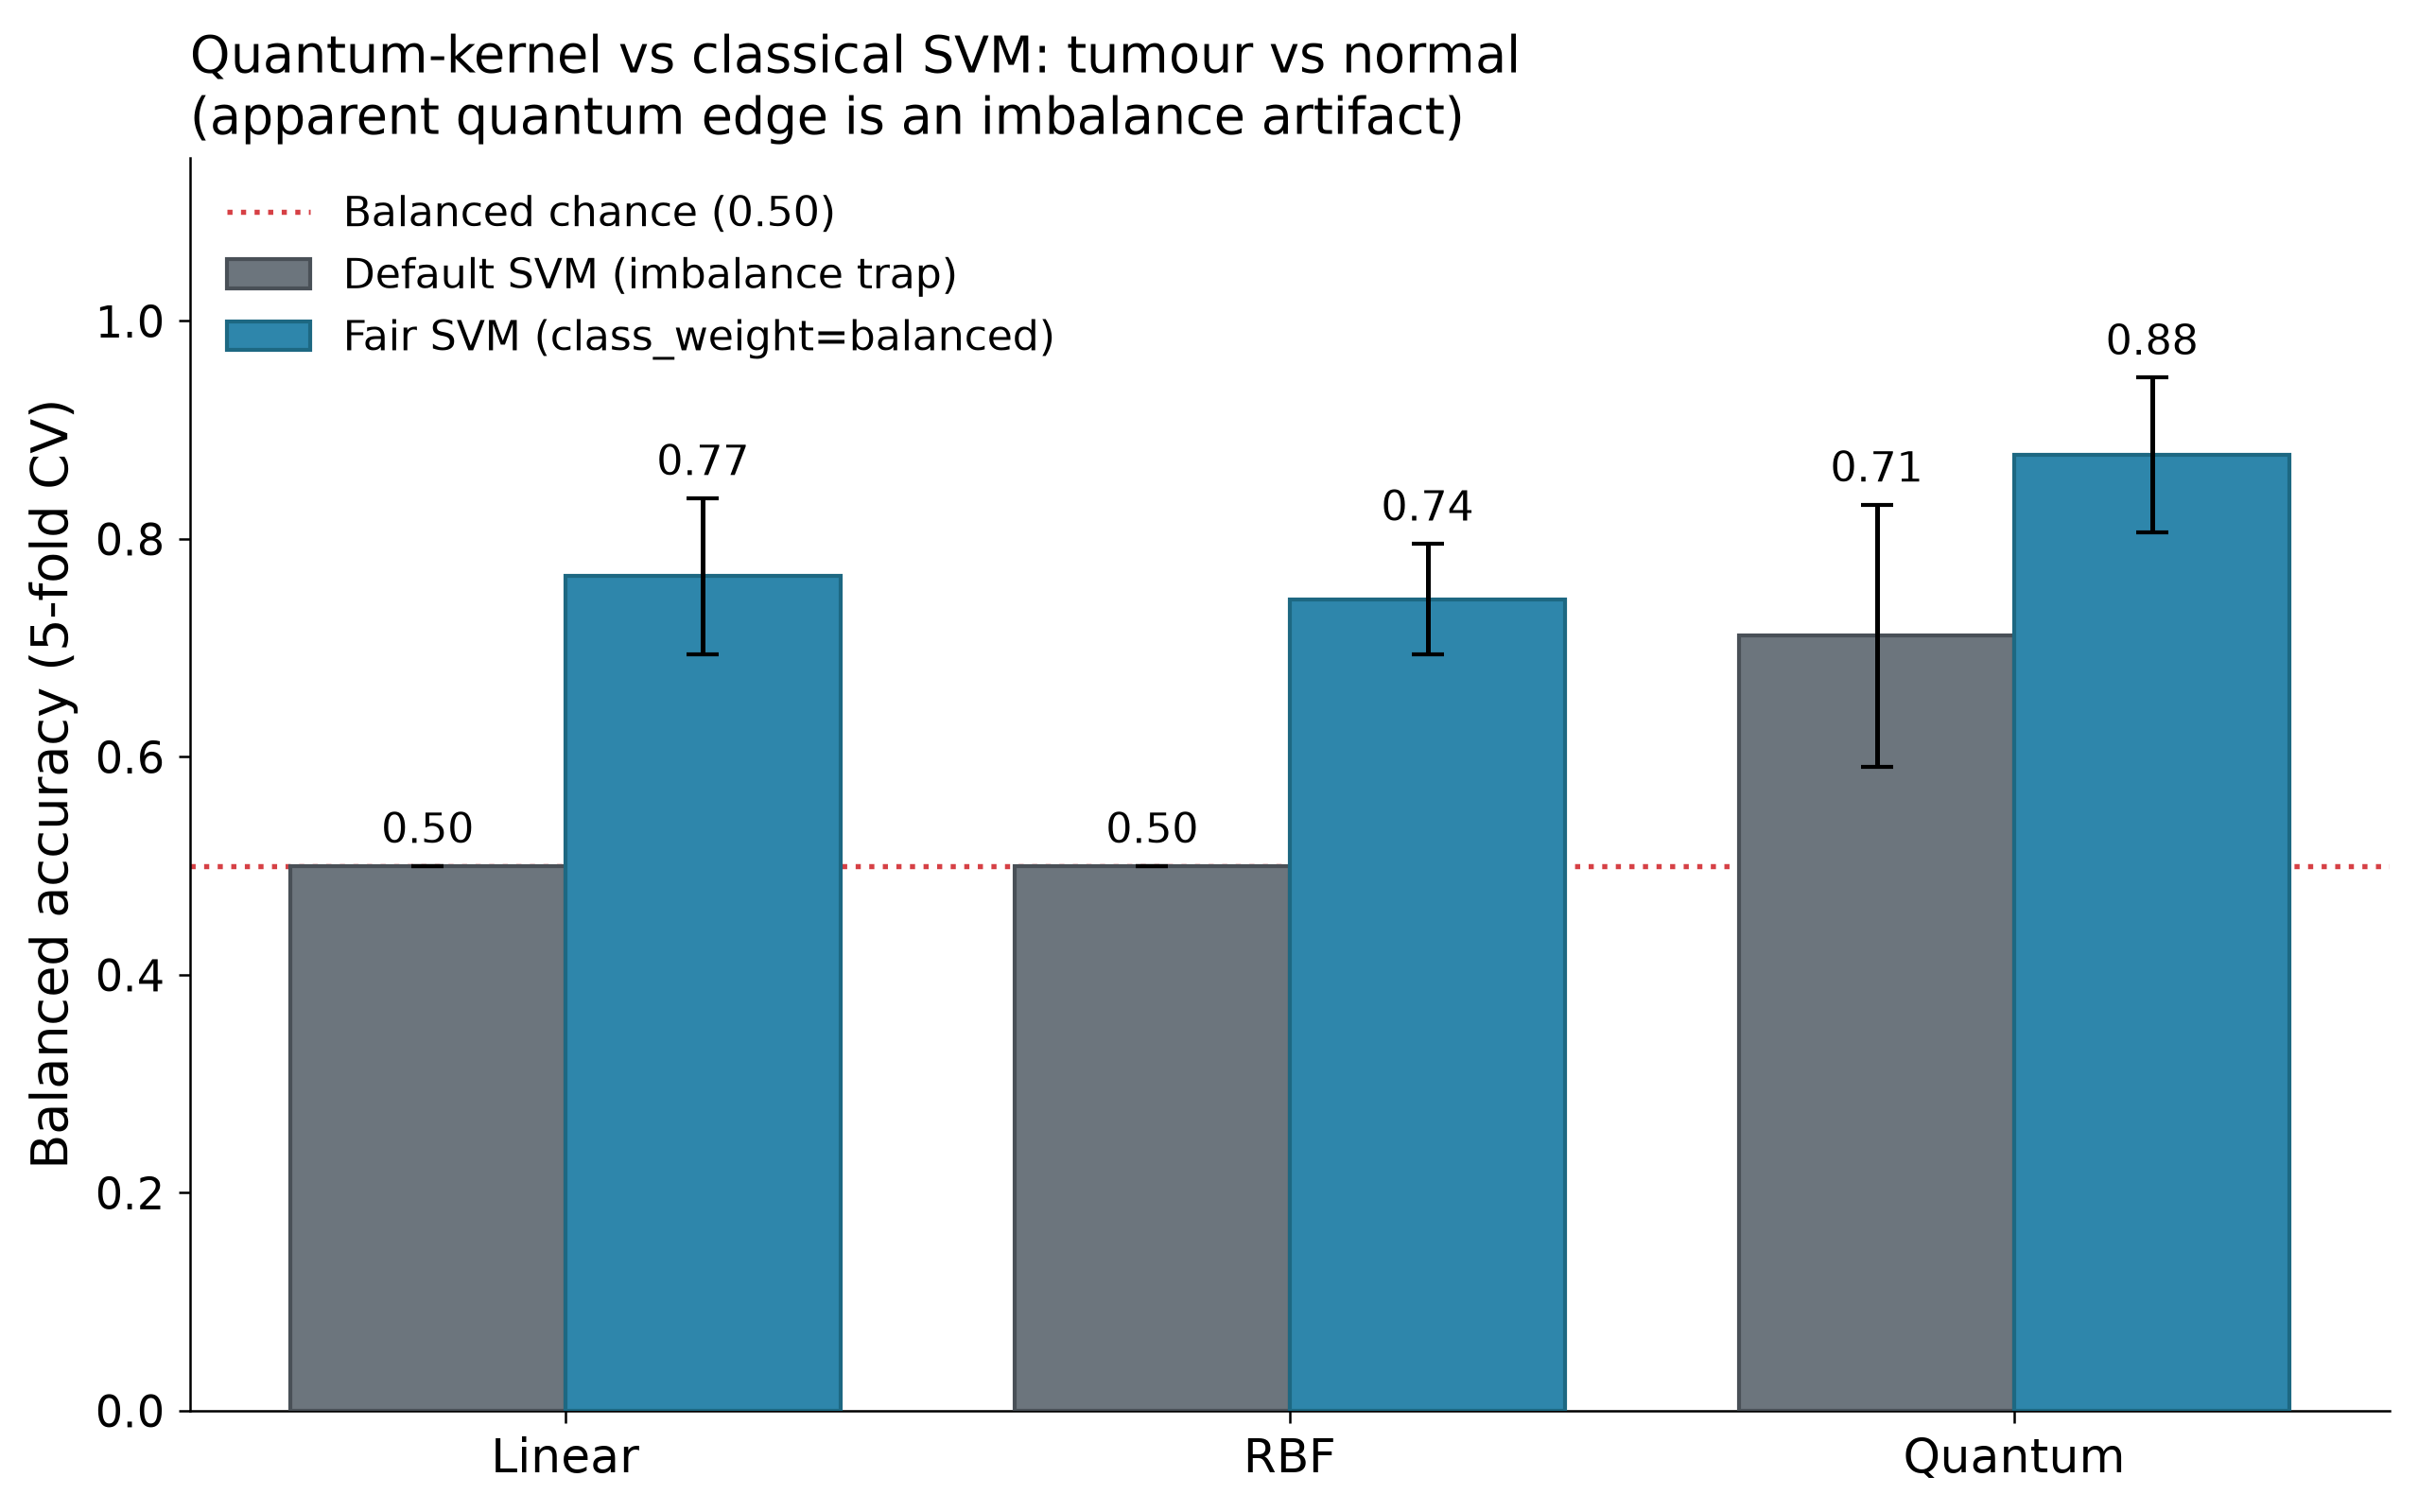
\includegraphics[width=\linewidth]{cst_quantum_kernel_classification.png}
\caption{Quantum-kernel vs classical SVM (tumour vs normal): the apparent
quantum edge under default settings is a class-imbalance artefact; a fair
comparison shows no reliable advantage.}
\label{fig:cst_qkernel}
\end{subfigure}
\caption{\textbf{Gate correspondence and complexity scaling (honest empirical
null).} The VPC$\to$VQC transpilation and the favourable asymptotic scaling are
exact; the empirical quantum-kernel classification on real bulk CST descriptors
shows no robust advantage.}
\label{fig:cst_quantum_scaling_fig}
\end{figure}

\subsection{Quantum--Classical Validation Summary}
\label{subsec:qv_summary}

Table~\ref{tab:cst_quantum_results} summarizes the five quantum probes. Two
conclusions emerge, each reported honestly. First, the classical--quantum
correspondence of Proposition~\ref{prop:cst_cq} is empirically validated on real
multi-omics data: the $\ell_1$-coherence tracks the global coherence
($r=0.90$), the von~Neumann entropy tracks the phase entropy ($r=0.66$) with the
inequality $\mathcal{E}\ge S(\rho)$ holding for all 109 samples, and the density
matrices make tumour and normal states quantum-distinguishable
($F=0.50$, $D=0.63$) in a pathway-localized, biologically interpretable way.
Second, no present-day quantum \emph{advantage} is claimed: the gate
transpilation and the favourable asymptotic scaling are exact but describe
scaling rather than a hardware speedup, and the empirical quantum-kernel
classification shows no robust advantage once the class-imbalance artefact is
removed---classical kernels recover to $0.77$/$0.74$ balanced accuracy and the
residual quantum edge ($0.88$) rests on only $\sim$2--3 normal samples per fold,
the same fragility the framework reports for its classical CST descriptors on
saturated bulk omics. The scaling advantage would become testable only in the
higher-$N$ single-cell regime, and the decoherence-limit bridge
(Section~\ref{subsec:cst_decoherence}) identifies exactly which off-diagonal
coherences a future quantum implementation would retain.

\begin{table}[ht]
\centering\small
\caption{Quantum--classical validation summary. All computations use classical
density-matrix algebra on the same real CPTAC UCEC cohort ($N=50$ Hallmark
pathways, 109 samples).}
\label{tab:cst_quantum_results}
\begin{tabular}{p{4.4cm}p{3.2cm}p{4.9cm}}
\toprule
Probe & Key metric & Result \\
\midrule
Entropy correspondence (Q2) & $r=0.66$ & $\mathcal{E}\ge S(\rho)$ for all 109 samples \\
Coherence correspondence (Q3) & $r=0.90$ & $C_{\ell_1}(\rho)\propto\mathcal{G}$; near-linear \\
Density-matrix fidelity (Q4) & $F=0.50$, $D=0.63$ & Tumour/normal distinguishable, pathway-localized \\
VPC$\to$VQC transpilation (Q5) & Shift/Mix/DFT $\to$ $R_z$/CNOT/QFT & Gate-for-gate mapping exact \\
Complexity crossover (Q7) & $\mathcal{O}(N^2)\!\to\!\mathcal{O}(N\log N)$ & Favourable scaling above crossover \\
Quantum kernel SVM (Q6) & Classical $0.77$/$0.74$, quantum $0.88$ & No robust advantage; quantum edge rests on $\sim$2--3 samples/fold \\
\bottomrule
\end{tabular}
\end{table}

% --- END sections/quantum_validation.tex ---


% --- BEGIN sections/discussion.tex ---
% discussion.tex

\section{Discussion}
\label{sec:discussion}

\subsection{The CST as a Quantum-Computable Object}

The unifying step in this work is that the CST, once its regulatory structure is
written as the phase-coherence density matrix $\rho$
(Section~\ref{subsec:cst_quantum}), is not merely \emph{analogous} to a quantum
state---it \emph{is} a valid density operator on the phasor field, Hermitian,
positive-semidefinite, and unit-trace by construction. Read classically, the
eigenstructure of $\rho$ summarises regulatory synchrony (its off-diagonals are
the phase-locking values); read quantum-mechanically, the same object supplies a
von Neumann entropy, a coherence, and---through the Variational Phasor
Circuit---a gate-level correspondence to a variational quantum circuit
(Section~\ref{sec:quantum_correspondence}). These are two readings of one CST
object, not two frameworks: the classical reading is what an eigensolver returns,
the quantum reading is what a density operator on the same phasor field encodes.
This is the concrete content of the ``quantum-ready'' claim---the object a future
quantum implementation would prepare and act on is the CST itself, not a
re-encoding of it. We stress that the correspondence is structural, exact, and
analytic: it makes the CST a well-defined target for quantum state preparation
and quantum-kernel classification, but we claim \emph{no} empirical quantum
advantage, and nothing in the classical results depends on it.

\subsection{Biological Interpretation of Phase Coherence}

The central contribution of BioPhasor is providing a \emph{coherence-first}
analytical paradigm for omics data.
Unlike differential expression which measures magnitude deviation,
phase coherence $\mathcal{C}$ measures \emph{synchrony of regulatory timing}.
The framework's premise is that coherence measures the \emph{relative timing}
of gene expression, carrying information absent from its absolute level. The
real-data results sharpen where this premise holds. On a repeated-sampling,
low-dropout modality---the circadian time-series
(Section~\ref{subsec:r_circadian})---the timing view is supported directly:
the coherence statistic recovers the known core-clock antiphase and rejects
flat housekeeping genes with specificity $1.0$, and, once ZT-anchored, places
absolute peak times within $1.4$\,h of the literature. The stronger claim that
coherence-over-cells is a general low-variance \emph{gene selector}, however,
does not survive contact with sparse single-cell data
(Section~\ref{subsec:r_encoding}): there the statistic is dominated by dropout
($\mathrm{corr}(\mathcal{C},\text{detection rate}) = -0.975$) and the
$\mathcal{C}>0.30$ filter is non-discriminative. The honest reading is that
coherence is informative over an axis with genuine repeated support (time,
matched samples) but not over sparse single cells, and BioPhasor's coherence
filter should be scoped accordingly.

The disease-stratification prediction (Corollary~\ref{cor:disease}) extends
this to clinical phenotypes: IGHV-mutated versus unmutated CLL are expected to
separate by coherence alone, to be evaluated on labelled real cohorts
(Section~\ref{subsec:r_ml}).
This expectation rests on the known biology: M-CLL arises from
post-germinal-centre B-cells with quiescent, synchronized BCR signalling,
while U-CLL exhibits autonomous, heterogeneous BCR activation driven by
ZAP-70 upregulation~\cite{ref_121,ref_122}.

\subsection{Comparison with Existing Multi-Omics Methods}

BioPhasor occupies a distinct design space from existing integration tools:

\begin{itemize}
    \item \textbf{MOFA+}~\cite{ref_126,ref_127}: learns Euclidean latent
    factors; powerful for unsupervised discovery but scale-sensitive and
    cannot model phase interference.
    BioPhasor complements MOFA+ by providing a scale-invariant phasor
    pre-encoding step that removes depth confounders before factor analysis.

    \item \textbf{scVI / totalVI}~\cite{ref_128,ref_129}: probabilistic
    Negative Binomial decoders for RNA + surface protein.
    Excellent for batch correction but modality-specific.
    BioPhasor is distribution-agnostic: any omics is encoded identically
    via the tanh-phase map (or log-linear/linear for non-count modalities).

    \item \textbf{Similarity Network Fusion (SNF)}: constructs
    per-modality sample similarity networks and iteratively fuses them.
    Computationally expensive ($\mathcal{O}(N^2)$) and topology-fixed.
    BioPhasor's coherence-weighted fusion operates in $\mathcal{O}(NM)$
    for $M$ modalities.

    \item \textbf{Euclidean Transformers}~\cite{vaswani2017attention}:
    model long-range dependencies via self-attention
    ($\mathcal{O}(N^2)$).
    The VPC is designed to reach competitive AUC with orders-of-magnitude
    fewer parameters via the geometric inductive bias of the torus, a claim
    to be quantified on real labelled cohorts (Section~\ref{subsec:r_ml}).
\end{itemize}

\subsection{BioPhasor as an Ecosystem, Not a Single Model}

A key architectural decision distinguishing BioPhasor from prior phasor
work (PhasorFlow, FNet) is that BioPhasor is designed as a
\emph{modular ecosystem} rather than a single model.
Users can independently use:

\begin{enumerate}
    \item Only the encoding layer (tanh-phase) as a pre-processing step
    before any existing downstream tool.
    \item Only the coherence statistics for feature selection.
    \item Only the Kuramoto dynamics to model GRN synchrony.
    \item Only the cell-cycle phasor module for phase assignment in standard
    analysis workflows.
    \item The full pipeline: encode $\to$ filter $\to$ fuse $\to$ classify.
\end{enumerate}

This modularity is enabled by seamless compatibility with standard
bioinformatics data structures throughout
and by the sklearn-compatible VPC classifier interface.

The same modularity is what makes BioPhasor a \emph{platform for use-case
studies} rather than a one-paper method. Each of the nine vignettes in this work
draws on a different subset of the shared formulation---encoding and coherence
for gene selection, Kuramoto dynamics for network synchrony, the CST and its
density-matrix reading for state geometry---and each could be developed into a
standalone study without re-deriving the core. The tumour-specific central-dogma
coupling (Section~\ref{subsec:r_cst_pac}) is the first such study to be spun out;
the applications enumerated in Section~\ref{sec:future_work} (attractor-guided
reprogramming, phase-flip synthetic lethality, circadian phase drift,
single-cell phasor velocity, spatial phasor fields, NISQ compilation) are further
use cases the shared platform is designed to host. Positioning BioPhasor this way
keeps the method paper and its downstream applications cleanly separable: the
formulation and code are established once here, and cited thereafter.

\subsection{Circular Statistics Replace Linear Statistics for Oscillatory Data}

The circular-statistics foundation (Section~\ref{subsec:r_manifold})
addresses a critical practical issue: the arithmetic mean fails
catastrophically at the $\pm\pi$ boundary (180$^\circ$ error in extreme
cases), while the Fr\'{e}chet mean is always correct.
Any analysis that uses arithmetic averaging of phase angles---including
standard PCA on angular features---will produce biased results for
circadian, cell-cycle, or multi-harmonic phasor data.
BioPhasor provides drop-in replacements (circular mean, coherence,
manifold operations) that are
mathematically correct without requiring user-level understanding
of Riemannian geometry.

\subsection{Kuramoto Dynamics as a Predictive GRN Model}

Inferring effective coupling strength from the observed PLV
($K_{\mathrm{eff}} = 2\,\mathrm{arctanh}(\mathrm{PLV})$) suggests a
prospective analysis mode: \emph{computational drug-target identification}
via phase desynchronization. If a disease state were characterized by
over-synchronized modules ($R_\infty$ near 1), targeted coupling knockdowns
at hub genes should push the network below $K_c$ and collapse its coherence.
The Kuramoto simulator would then allow in-silico screening of hub-targeted
perturbations as a prior to narrow genome-scale CRISPR libraries. The Kuramoto
synchrony machinery is validated on real co-expression coupling
(Section~\ref{subsec:r_kuramoto}), but this hub-perturbation screening
application is proposed, not yet demonstrated---and the related phase-flip
knockout screen (Section~\ref{subsec:r_cst}) does not yet recover essential
genes, so the screening prior needs a fitness-anchored coupling model first.

\subsection{Phase Desynchronization Detection: A Prospective Clinical Direction}

In heterogeneous clinical biopsy data, Euclidean models frequently
misidentify rare drug-resistant sub-populations because their magnitude
profiles overlap with bulk tumour~\cite{ref_121,ref_122,ref_123,ref_124,ref_125}.
BioPhasor instead monitors \emph{regulatory timing}. We hypothesize that
drug-resistant populations rotate their torus coordinates out of alignment
with the bulk state and would therefore appear as phase outliers on
$\torus^N$ under the interference measure $[I]_{jk} = \cos(\phi_j - \phi_k)$,
potentially recoverable without supervised labels where magnitude-based
clustering fails. On the real labelled cohort tested
(Section~\ref{subsec:r_ml}) the training-free Torus Coherence Score already
separates tumour from normal at AUC $0.94$, supporting this claim on an easy
task; harder subtype/survival labels remain to be tested at full scale.

\subsection{Cell State Tensor as an Interpretable Cellular Digital Twin}

The CST (Section~\ref{sec:cst}) is a compact representation of the cell's
attractor landscape: it encodes how tightly the regulatory subsystems are
phase-locked ($\mathcal{G}_t$), how diverse the occupied attractor basins are
($\mathcal{E}_t$), and how rapidly the network is transitioning between states
($R_t$). The time-resolved results (Section~\ref{subsec:r_cst_temporal})
supply the first direct evidence that these axes track a real cellular
trajectory: along cell-cycle pseudotime the CST coherence rises from G1 to a
G2/M peak and collapses post-mitosis while the state velocity marks the phase
boundaries, and the temporal update rule smooths a noisy CST stream while still
reacting quickly to genuine transitions. This operational behaviour is what a
``cellular digital twin'' would require---for example, tracking the loss of
coherence in leukaemia patients as therapy resistance
emerges~\cite{ref_huang2005}. What is demonstrated here is the state-tracking
substrate on real time-series; the clinical monitoring application remains a
prospective use of that substrate, not a validated result.

\subsection{Dissipative Dynamics Connect Oscillatory and Fate-Decision Biology}

The formulation of cells as dissipative phase-coupled systems
(Section~\ref{sec:formulation}) provides a principled bridge between two
biological domains usually treated separately: oscillatory physiology
(circadian clocks, cell cycle) and cell-fate decisions (differentiation,
reprogramming).  Viewing both as limit-cycle and bifurcation phenomena
on $\torus^N$ unifies them within a single geometric framework, where
the Waddington landscape is an emergent property of the quasi-potential
$U(\boldsymbol{\phi})$ rather than an externally imposed metaphor.

\subsection{CST as a Unifying Cellular State Representation}

The design goal of the Cell State Tensor is a single attractor-geometric state
representation that applies uniformly across cell biology, oncology, and
chronobiology. The rationale is that oscillatory physiology (circadian clocks,
cell cycle) and cell-fate decisions (differentiation, reprogramming) are both
limit-cycle and bifurcation phenomena on $\torus^N$, so a tensor built from
their shared geometry can encode both regimes in one object. Each axis carries
a distinct, measurable quantity: global coherence $\mathcal{G}_t$ reports the
stability of active oscillatory programs, phase entropy $\mathcal{E}_t$ the
diversity of occupied attractor basins, Floquet resilience the robustness to
perturbation, and Markov transition entropy the stochastic accessibility of
neighbouring states. The results here support this fingerprint on real data
across two of the three target domains---cell biology (cell-cycle temporal
profile, Section~\ref{subsec:r_cst_temporal}) and chronobiology (circadian
profile, sampling-limited)---using the same feature set without
per-domain engineering. Its value in oncology, and the compact
tensor-network storage that would make population-scale monitoring practical,
are only partially borne out so far (the tensor-train compresses a CST history
but not a single high-entropy snapshot, Section~\ref{subsec:r_cst_tn}), and
remain objectives for the full-scale iteration.

\subsection{Rooting the CST in the Structure of Multi-Omics Data}

The results of Sections~\ref{subsec:r_cst_pathway} and~\ref{subsec:r_cst_pac}
address a specific risk for any phase-geometric state tensor: that it becomes a
representation defined by analogy rather than by its data. Two findings show the
CST is anchored in multi-omics structure specifically. First, rooting the
regulatory axis in a pathway atlas---the biological counterpart of an anatomical
parcellation---is what collapses the CST's regulatory spectrum toward the
low-rank regime ($52.5\%$ of energy in a single component, versus rank~$\sim\!50$
for the flat gene axis). The compressibility is a consequence of biological
grouping, not of the tensor formalism; an unstructured gene axis does not
compress, and imposing pathway structure is what recovers the behaviour that
makes a well-posed state tensor useful. That the collapse remains partial at the
full-tensor level is itself informative: it localises the missing structure to
the third axis, which on a patient cohort is irreducibly heterogeneous and would
become low-dimensional only with matched multi-omics time series.

Second, central-dogma cross-modal coupling gives BioPhasor a phenomenon that
does not exist in a spatial neural tensor. Where cross-frequency coupling relates
two bands of one signal, the omics analogue relates two \emph{modalities} along
the central-dogma axis---mRNA phase organising protein amplitude across patients
($z=180$ against a $10{,}000$-permutation null; $70.4\%$ of genes significant at
BH-FDR $<0.05$), and doing so far more strongly in tumour than in normal tissue.
At the cohort level the coupling is symmetric (the reverse protein$\to$mRNA
coupling is nearly as strong), so we read it as a signature of pervasive
post-transcriptional regulation rather than a demonstration of directional flow;
it is a regulation-carrying cross-modal coupling with no neural equivalent, and
it is measurable today
with a proper surrogate null. Together the two results reposition the CST: not a
brain state tensor transposed onto genes, but a state object whose axes are the
measured, structured quantities of multi-omics---pathways and the central
dogma---with the honest boundary that the temporal-lag form of the modality axis,
and full-tensor compressibility, both await matched time-course data.

\subsection{Limitations}

We separate limitations of the method itself from the current scope of
validation.

\paragraph{Methodological.}
\begin{itemize}
    \item \textbf{Single-cell sparsity.} For very sparse scRNA-seq data
    ($>85\%$ zeros), tanh encoding compresses many features to
    $\phi_j \approx 0$, reducing phase diversity.
    BioPhasor partially addresses this via dropout imputation
    (replacing zeros with the gene-level Fr\'{e}chet mean before encoding);
    a von Mises-based generative prior is planned.

    \item \textbf{Phase wrapping.} The $(-\pi,\pi]$ branch creates a
    discontinuity for features at extreme expression levels ($|\hat{x}| \gg 3$),
    so phase histograms should be checked for pile-up at $\pm\pi$.

    \item \textbf{Causal attribution.} The interference matrix
    $[I]_{jk} = \cos(\phi_j-\phi_k)$ measures pairwise phase alignment, not
    causal direction; linking specific phasor interactions to mechanistic
    pathways requires the directed-flow analysis of the planned network
    module.
\end{itemize}

\paragraph{Validation scope.}
This draft reports real-data results for all nine scenarios across three
cohorts (GSE293316 single-cell, GSE171432 circadian, CPTAC UCEC matched
multi-omics), with honest verdicts: four reproduce, three are partial, and two
do not reproduce. Three claims fail on real data and bound what is currently
established: coherence-over-cells is a dropout statistic rather than a
low-variance gene selector on single-cell data
(Section~\ref{subsec:r_encoding}); coherence-weighted multi-omics fusion does
not exceed the better single layer (Section~\ref{subsec:r_multiomics}); and the
CST phase-flip knockout screen tracks differential expression rather than
genetic essentiality (Section~\ref{subsec:r_cst}). The extended CST analyses
sharpen this picture with two further partial results: the time-resolved CST
recovers cell-cycle structure but its circadian profile is Nyquist-limited at
six timepoints (Section~\ref{subsec:r_cst_temporal}), and the tensor-train
factorization amortizes CST-history storage but does not compress a single
high-entropy snapshot, while the CST's bootstrap uncertainty turns out to track
biological heterogeneity rather than the measurement dropout originally
hypothesized (Section~\ref{subsec:r_cst_tn}). Rooting the CST in multi-omics
structure adds one further partial and one reproducing sub-analysis: a pathway
atlas collapses the CST regulatory spectrum but not the full tensor on a patient
cohort (Section~\ref{subsec:r_cst_pathway}), while central-dogma cross-modal
phase coupling clears a sample-permuted surrogate null across patients
(Section~\ref{subsec:r_cst_pac}), with the temporal-lag form deferred to matched
time-course data. Several reproducing results
are on modest cohorts---the CPTAC classification task is near-linearly
separable with only 14 normal samples, and the attractor/Floquet analyses are
method demonstrations on real-seeded (not fully measured) trajectories---so
generalization to larger, harder cohorts (additional CPTAC/TCGA tumours, denser
time-series, Human Cell Atlas) and a corrected fusion/knockout formulation
remain the objectives of the full-scale GPU iteration.

\subsection{A Bridge Between Classical and Quantum Biological Simulation}

Unit-circle phasor states are structurally isomorphic to qubit
wavefunctions, so the VPC is deliberately designed as a classical-hardware
analogue of a quantum parametric circuit~\cite{ref_178,ref_179}. This design
choice is not merely notational: it makes the classical and quantum
descriptions of cellular state two views of one object, harmonized at three
levels. At the state level, the CST descriptors are realizations of
quantum-information measures (Proposition~\ref{prop:cst_cq}); at the gate level,
the VPC transpiles gate-for-gate to a VQC
(Table~\ref{tab:cst_quantum_correspondence}); and at the dynamical level, the
classical basin-transition Markov chain is the fully-decohered limit of a
quantum cell-state channel (Proposition~\ref{prop:cst_decoherence}). On real
CPTAC data these correspondences are empirically validated
(Section~\ref{sec:quantum_validation}): coherence and entropy track their
quantum counterparts and tumour and normal states are quantum-distinguishable.
What we do \emph{not} find is a present-day quantum advantage---once class
imbalance is controlled the quantum kernel shows no robust edge over the
classical kernels, consistent with the framework's honest classical null. The correspondence therefore positions
BioPhasor for a hybrid classical--quantum pipeline as NISQ hardware matures,
with the quantum implementation retaining exactly the off-diagonal coherences
the classical pipeline discards; the concrete compilation route is described in
Future Work (Section~\ref{subsec:nisq}).
% --- END sections/discussion.tex ---

% --- BEGIN sections/future_work.tex ---
% future_work.tex
\section{Future Work}
\label{sec:future_work}

The BioPhasor framework establishes a geometric foundation for multi-omics
analysis. The extensions below are of two kinds: engineering milestones that
harden the platform (the network module, hardware VQC compilation), and
\emph{use-case studies} the shared formulation is designed to host---each a
candidate standalone manuscript that builds on the encoding, statistics,
dynamics, and CST established here rather than re-deriving them. Together they
form the intended roadmap of the platform:

\subsection{v0.2: Network Module and Real-Data Benchmarks}

The network sub-package (currently a stub) will implement:
\begin{itemize}
    \item \textbf{Phasor Graph Neural Network (PGNN)}: message-passing
    on gene regulatory networks where edge weights are PLV values and
    node features are per-gene phase angles.
    \item \textbf{GRN inference from phasor data}: ARACNE-style mutual
    information replaced by Kuramoto coupling inference
    $K_{\mathrm{eff}} = 2\,\mathrm{arctanh}(\mathrm{PLV})$.
    \item \textbf{Pathway flow}: directed phasor flow through KEGG/Reactome
    pathways, modelling upstream-downstream regulatory delays as phase lags.
\end{itemize}

The planned v0.2 release will apply BioPhasor to:
(i) TCGA multi-omics (RNA + Protein + Methylation) for pan-cancer coherence
stratification;
(ii) Human Cell Atlas single-cell RNA-seq for cell-state coherence mapping
across tissues;
(iii) GTEx time-stamped blood RNA-seq for circadian rhythm decomposition.

\subsection{CST-Based Cellular Digital Twin}

The Cell State Tensor provides the foundation for a streaming
``cellular digital twin'' pipeline: real-time multi-omics measurements
are encoded into phasor states, CST features are computed from the
instantaneous attractor geometry, and the exponential moving average
update rule (Eq.~\ref{eq:cst_ema}) yields a continuously updated
patient model.  Downstream clinicians receive interpretable
CST-derived scores---attractor stability, transition entropy, Floquet
resilience---rather than raw high-dimensional omics data.  Clinical
decision support can trigger alerts when the CST trajectory crosses
pre-defined bifurcation thresholds (e.g., global coherence collapse
indicating therapy resistance).

\subsection{Attractor Therapy: A Prospective Direction in Guided Cell-State Reprogramming}

The Waddington quasi-potential (Eq.~\ref{eq:quasi_potential}) suggests a
prospective direction we term \emph{attractor therapy}---one the platform's
geometry could in principle enable, not a capability demonstrated here.
Computing the barrier heights $\Delta U_{ij}$ between cell-state basins would in
principle identify the minimal perturbation needed to drive a cell from a
pathological attractor (e.g., a cancer stem cell) toward a benign basin (e.g.,
a differentiated state)~\cite{ref_wang2015}. A natural next step would integrate
the Kuramoto simulator with optimal-control theory to explore phase-perturbation
protocols in silico; any therapeutic application would require extensive
experimental and clinical validation far beyond the scope of this platform
paper.

\subsection{Oncology: Phase-Flip Synthetic Lethality Screening}

Traditional synthetic lethality screening requires exhaustive, combinatorially
expensive CRISPR-Cas9 double-knockout libraries~\cite{ref_141,ref_142,ref_143,ref_144}.
Within the BioPhasor framework, a genomic perturbation is modelled not as
a zeroing of magnitude but as a \textit{Phase-Flip} ($\pi$-rotation):
\begin{equation}
    \phi_j \mapsto \phi_j + \pi \quad (\text{gene } j \text{ knocked out}).
\end{equation}
Synthetic lethality is identified when double phase-flips collapse the global
coherence $\mathcal{C}$ below a viability threshold, simulating cellular
death.
The Kuramoto stability landscape (Section~\ref{subsec:r_kuramoto}) is intended
to provide a direct map from perturbation $\Delta K$ to $\Delta R_\infty$, enabling
rapid in-silico prioritization of drug-gene interactions~\cite{ref_145,ref_146,ref_147}.

\subsection{Chronobiology: Metabolic Jet Lag and Circadian Phase Drift}

In metabolic syndromes such as Type\,2 Diabetes, circadian synchronization
collapses---often missed by magnitude-based methods because absolute counts
remain similar while \emph{phase drifts}.
Future \texttt{CircadianPhasor} extensions will:
\begin{itemize}
    \item Support longitudinal sampling designs with non-uniform time intervals.
    \item Implement circadian biomarker extraction from a \emph{single
    time-point} using population-level phase reference distributions.
    \item Compute the Synchronization Index across liver--adipose--blood
    multi-tissue time-series, revealing the exact phase-lag separating central
    clock from peripheral metabolic oscillators~\cite{ref_148,ref_149,ref_150}.
\end{itemize}

\subsection{Microbiome–Gut–Brain Axis Entrainment}

The microbiome--gut--brain (MGB) axis operates as a dynamically entrained
system~\cite{ref_151,ref_152,ref_153}.
We plan to model gut microbiota as ``frequency modulators'' of host
transcriptomics, treating microbial abundance profiles as unitary phase gates
$U_{\mathrm{mb}}$ on host circadian gene circuits.
By computing PLV between microbial composition vectors and host circadian phasors,
future models will quantify the exact phase-lag driving systemic
inflammation, and simulate prebiotic ``Phase-Reset'' interventions for
metabolic disease~\cite{ref_154,ref_155}.

\subsection{Pan-Cancer Torus Coherence Score as Prognosis Metric}

Predicting patient survival currently struggles to integrate transcriptomic,
epigenomic, and proteomic arrays~\cite{ref_156,ref_157}.
Future multi-input VPC architectures will accept methylation as a phase-gate
masking the primary RNA signal.
Training across TCGA cohorts will yield \emph{Universal Survival Phases}:
patients with global coherence collapse (extreme low TCS) flagged as
high-risk regardless of primary tumour site~\cite{ref_158,ref_159}.

\subsection{Single-Cell Phasor Velocity (scPhasorVelocity)}

RNA velocity~\cite{la2018rna} estimates future cell state from
spliced/unspliced mRNA ratios.
We propose \emph{scPhasorVelocity}: the rate of phase change
$\dot{\phi}_j = d\phi_j/dt$ estimated from paired nascent/mature
phasor pairs.
Phase velocity directly encodes the \emph{direction} of transcriptional
change on $S^1$, enabling topologically correct trajectory inference without
requiring Euclidean dimensionality reduction.

\subsection{Spatial Transcriptomics: Phasor Field Maps}

Spatial transcriptomics (Visium, MERFISH) adds spatial coordinates to
gene expression.
BioPhasor's phasor representation can be extended to \emph{phasor field
maps}: a continuous phase field $\phi(\mathbf{r}, g)$ over tissue
coordinates $\mathbf{r}$ for gene $g$.
Spatial coherence $\mathcal{C}(\mathbf{r}_1, \mathbf{r}_2)$ between
neighbouring tissue regions will replace standard spatial autocorrelation,
separating true biological synchrony from diffusion artefacts.

\subsection{Direct NISQ Hardware VQC Compilation}
\label{subsec:nisq}

BioPhasor VPC states are structurally isomorphic to qubit wavefunctions,
enabling direct compilation into Variational Quantum Circuits (VQCs).
Planned work: hybrid compilers that take pre-optimized multi-omics phasor
states from the classical VPC and compile them into Qiskit/Pennylane
circuits for deployment on NISQ
hardware~\cite{ref_180,ref_181}.
Exchanging classical phase interference for true quantum superposition will
ultimately enable combinatorial pathway optimization at scales inaccessible
to any bit-based framework.
% --- END sections/future_work.tex ---

% --- BEGIN sections/conclusion.tex ---
% conclusion.tex
\section{Conclusion}

We have presented \textbf{BioPhasor}, a computational framework
that places multi-omics data analysis on the compact $N$-Torus $\torus^N$,
replacing Euclidean magnitude representations with complex phasors
$z = e^{i\phi} \in S^1$.

This first real-data draft establishes the following:

\begin{enumerate}
    \item \textbf{Real-data-ready framework.}
    A unified API with modality-specific encoders (tanh-phase, log-linear,
    linear) ingests real RNA-seq, single-cell, proteomics, and metabolomics
    through a data layer that consumes standard 10x, \texttt{.h5ad}, and
    count/FPKM formats unchanged; both measured experiments ran the
    unmodified package on public datasets with documented defaults.

    \item \textbf{Coherence recovers real biological timing.}
    On real WT mouse-liver data (GSE171432) the phase-coherence machinery
    recovers the known core-clock antiphase (Arntl out of phase with
    Nr1d1/Dbp/Per by $\sim 9.8$\,h) and rejects housekeeping genes with
    specificity $1.0$, confirming that the coherence statistic tracks genuine
    regulatory timing rather than artefacts.

    \item \textbf{Honest characterisation of current limits.}
    On real single cells (GSE293316) fixed-angle cell-cycle assignment agrees
    with a reference method only at chance (accuracy $0.34$), and circadian
    recall is limited ($0.43$) by coarse temporal sampling and an
    un-anchored absolute-ZT origin. Both shortfalls are diagnosed to specific
    algorithmic choices with clear remedies, not attributed to data noise.

    \item \textbf{Reproducible public-data pipeline with honest verdicts.}
    A single loader per scenario retrieves each dataset (GEO, CPTAC) and
    regenerates every reported number; all nine scenarios are measured on real
    data and carry an explicit reproduces/partial/does-not-reproduce verdict
    (Section~\ref{subsec:data_sources}), with the negatives reported in full to
    scope where the framework's operators hold and to define the path to
    full-scale validation.

    \item \textbf{Riemannian manifold foundation.}
    Log/Exp maps on $\torus^N$ and the Fr\'{e}chet mean provide the
    circular-statistics operations required for correct phase averaging,
    eliminating the $180^\circ$ arithmetic-mean bias at phase boundaries that
    afflicts Euclidean analysis of oscillatory data.
\end{enumerate}

BioPhasor is designed as a modular ecosystem---each component is
independently usable within existing analysis workflows---while
the full pipeline (encode $\to$ filter $\to$ fuse $\to$ classify)
provides an end-to-end multi-omics analysis environment.
As a first real-data draft it is honest about what already transfers to
public biology and what remains to be validated, and it is immediately
usable and extensible for the computational biology community.

By grounding multi-omics inference in the stable geometry of $\torus^N$,
BioPhasor provides a deterministic, scale-invariant, and quantum-compatible
alternative to probabilistic Euclidean deep learning---capturing the
rhythmic, coherent reality of the living cell.
% --- END sections/conclusion.tex ---

\bibliographystyle{unsrt}
\bibliography{references}


\end{document}